%%%%%%%%%%%%%%%%%%%%%%%%%%%%%%%%%%%%%%%%%
% Design based on a template by Roberto and following the format of
% the xmipp tutorials. In turn, they seem to be based on a template
% from http://www.latextemplates.com
%%%%%%%%%%%%%%%%%%%%%%%%%%%%%%%%%%%%%%%%%

%----------------------------------------------------------------------------------------
%	PACKAGES AND OTHER DOCUMENT CONFIGURATIONS
%----------------------------------------------------------------------------------------

\documentclass[12pt]{article} % Default font size is 12pt, it can be changed here
\usepackage[english]{babel}
\usepackage[utf8]{inputenc}
\usepackage{listings} % To include source code
\usepackage{caption}
\usepackage[htt]{hyphenat}
\usepackage{geometry} % Required to change the page size to A4
%\geometry{a4paper} % Set the page size to be A4 as opposed to the default US Letter
\usepackage{framed}
\usepackage{url}
\usepackage{graphicx} % Required for including pictures
\usepackage{natbib}
\usepackage{float} % Allows putting an [H] in \begin{figure} to specify the exact location of the figure
%\usepackage{hyperref}
\usepackage{menukeys}
\usepackage{array}
\usepackage{fancyhdr}
\usepackage{marvosym}%smileys\Smiley{} \Frowny{}
\usepackage{etoolbox}
\usepackage{listings}
\usepackage{makecell}
\usepackage{marginnote}
\usepackage{soul}
\usepackage[toc,page]{appendix}
\usepackage{caption}
%\usepackage{menukeys}
\usepackage{fancybox,framed}
\usepackage{xspace}
\usepackage{rotating}
\usepackage{gensymb}
\usepackage{vhistory}

%commands
\newcommand{\ffigure}[1]{{Fig. {\ref{#1}}}\xspace}
\newcommand{\ttable}[1]{{Table {\ref{#1}}}\xspace}
\newcommand{\scommand}[1]{{{\keys{#1}}}\xspace}
%definitions
\def\ccmask{CC\textsubscript{MASK}\xspace}
\def\ccp4{\textit{CCP4}\xspace}
\def\chimera{\textit{ChimeraX}\xspace}
\def\coot{\textit{Coot}\xspace}
\def\emringer{\textit{EMRinger}\xspace}
\def\modeller{\textit{Modeller}\xspace}
\def\molprobity{\textit{MolProbity}\xspace}
\def\validationCryoEM{\textit{Validation CryoEM}\xspace}
\def\phenix{\textit{PHENIX}\xspace}
\def\powerfit{\textit{PowerFit}\xspace}
\def\refmac{\textit{Refmac}\xspace}
\def\scipion{\textit{Scipion}\xspace}

\sethlcolor{yellow}

%\renewcommand{\hl}[1]{#1}
%pdflatex -jobname=students '\def\student{}\input{main}'
%pdflatex -jobname=teachers '\def\teachers{}\input{main}'
%  \ifdef{\teachers}
%  {Content for teachers}
%  {Content for students} 
\newcommand{\ttt}[1]{\texttt{#1}}
\newcommand{\iii}[1]{\textit{#1}}
\newcommand{\ra}{$\rightarrow$}
\pagestyle{fancy}
\fancyhf{}
\fancyhead[RO]{{Model Building}}
\fancyhead[LO]{Scipion}
%\fancyhead[RO]{{\leftmark}}
\fancyfoot[RO]{\thepage}

\linespread{1.2} % Line spacing

%\setlength\parindent{0pt} % Uncomment to remove all indentation from paragraphs
\newenvironment{command}{\tt\begin{quote}}{\end{quote}}
\newcommand{\comm}[1]{\texttt{#1}}

\newcommand{\imgfig}[3]{\begin{figure}[H]\centering \
\includegraphics[scale=#2]{images/#1} \caption{#3} \end{figure}}

\newcommand{\proto}[1]{\textit{\textbf{#1}}}
\newcommand{\popt}[1]{\textit{#1}}
\newcommand{\pval}[1]{\texttt{#1}}

\newcommand\tstrut{\rule{0pt}{2.4ex}}
\newcommand\bstrut{\rule[-1.0ex]{0pt}{0pt}}

\def \humanAdenoMap {7034}%5172

\begin{document}

%----------------------------------------------------------------------------------------
%	TITLE PAGE
%----------------------------------------------------------------------------------------

\begin{titlepage}

% New command for horizontal lines. Change thickness here.
\newcommand{\HRule}{\rule{\linewidth}{0.5mm}}

\center % Center everything on the page


\includegraphics{images/scipion_logo}

{\large Scipion Tutorial Series}\\[1.0cm]

\textsc{\LARGE National Center for Biotechnology}\\[0.5cm]
\textsc{\Large Biocomputing Unit}\\[0.15cm]

\HRule\\[0.3cm]
{ \huge \bfseries Model Building Basic}\\ % Title of your document
\HRule \\[0.35cm]
{\large \today}\\ % Date, change the \today to a set date if you want to be precise
\begin{center}
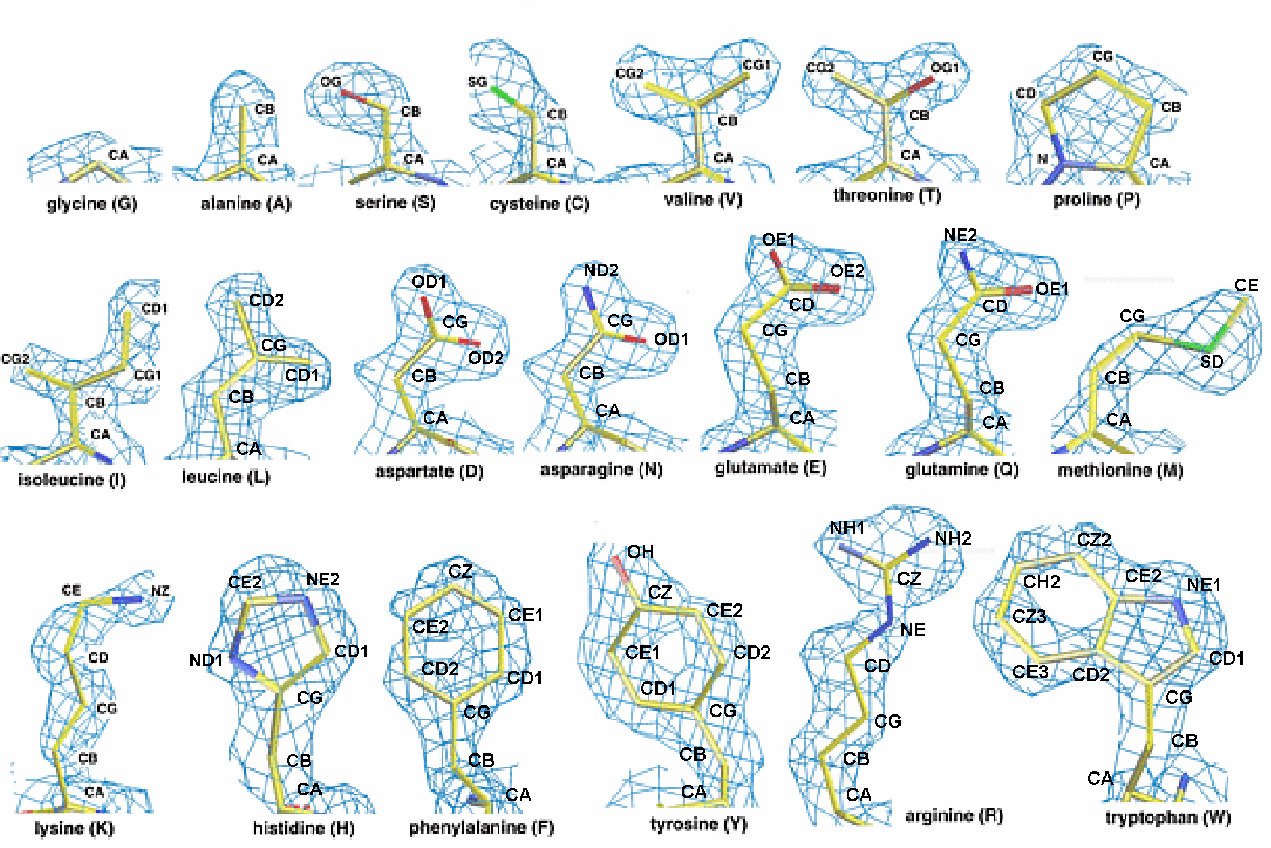
\includegraphics[width=0.70\textwidth]{{images/aadensity}}\\
Density for amino acid side chains from an experimental electron density map at 1.5 \AA~resolution \footnotesize{(http://people.mbi.ucla.edu/sawaya/m230d/Modelbuilding/modelbuilding.html)}
\end{center}

%\vfill % Fill the rest of the page with whitespace
%\begin{minipage}{0.4\textwidth}
\begin{flushright}
 \large
%\emph{Author:}\\
  \textsc{Roberto Marabini \& Marta Martínez} % Your name
\end{flushright}
%\end{minipage}

\end{titlepage}

\begin{versionhistory}
  \vhEntry{1.0}{11.15.2018}{MM|RM}{created for first model building workshop}
  \vhEntry{1.1}{01.30.2019}{MM}{added appendices and minor fixes}
  \vhEntry{1.2}{04.24.2019}{MM}{added atomstructutils, contacts and submission protocols}
  \vhEntry{1.3}{09.10.2019}{MM}{added map preprocessing protocols (create mask, and compute local Resolution and Sharpening) and \phenix validation cryoEM}
  \vhEntry{1.4}{30.10.2020}{MM}{migration to python3 and adaptation to \scipion version 3.0, replacement of Chimera by ChimeraX (new functionalities in model from template and map subtract), added other preprocessing tools ($DeepEMhancer$), added \phenix dock-in-map protocol, removed singularities for \phenix version 1.13, removed \powerfit protocol}
\end{versionhistory}\newpage

%----------------------------------------------------------------------------------------
%	OBJETIVOS
%----------------------------------------------------------------------------------------


\subsection*{Intended audience}
The recent rapid development of single-particle electron cryo-microscopy (cryo-EM) allows structures to be solved by this method at almost atomic resolutions.  Providing a basic introduction to model building, this tutorial shows the initial workflow aimed at obtaining high-quality atomic models from cryo-EM data by using \scipion software framework. %tomography in  electron microscopy with special emphasis in basic image processing. The tutorial requires matlab but does not assume any programing skills. 


\subsection*{We'd like to hear from you}

We have tested and verified the different steps described in this demo
to the best of our knowledge, but since our programs are in continuous
development you may find inaccuracies and errors in this text. Please
let us know about any errors, as well as your suggestions for
future editions, by writing to
scipion@cnb.csic.es.


\subsection*{Requirements}

This tutorial requires, in addition to \scipion, USCF~\chimera (\url{https://www.rbvi.ucsf.edu/chimerax/download.html}), the \ccp4 suite (\url{http://www.ccp4.ac.uk/download/#os=linux}) including \refmac and \coot, and the \textit{PHENIX suite} (\url{https://www.phenix-online.org/download/}). Basic knowledge of \chimera and \scipion is assumed. Warning: old versions of \refmac are not suitable for EM data.

\newpage


%----------------------------------------------------------------------------------------
%	TABLE OF CONTENTS
%----------------------------------------------------------------------------------------

\tableofcontents % Include a table of contents

\newpage % Begins on a new page instead of on the same page as the table of contents


\section{Introduction to Model building}

\subsection*{Definition}
 Model building is the process that allows getting the atomic interpretation of an electron density map. Although a electron density volume can be obtained from different methodologies, in this tutorial we focus in maps obtained by cryo-EM. As an example of these maps, \ffigure{fig:model_building_example} shows the input electron density map (a), as well as the output haemoglobin tetramer atomic model (b) obtained by the model building process. Since high quality atomic structures are essential to accomplish detailed mechanistic studies and to seek inhibitor drugs of macromolecules, the main aim of model building is obtaining reliable structures of these macromolecules. 
 

\begin{figure}[H]
 \centering
 \captionsetup{width=.8\linewidth}  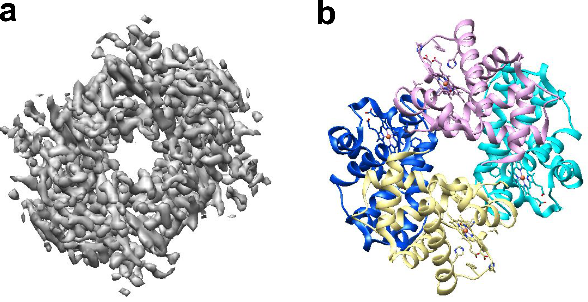
\includegraphics[width=0.6\textwidth]
  {{Images/Fig1.pdf}}
  \caption{Haemoglobin tetramer \citep{khoshouei2017}. a) Electron density map at 3.2\AA\ resolution obtained by Cryo-EM single particle analysis with Volta phase plate. b) Atomic structure model inferred from the electron density volume.}
  \label{fig:model_building_example}
  \end{figure} 
 

\subsection*{Relevance of cryo-EM map resolution}

Model building process is limited by the resolution of the starting cryo-EM density map. The higher the resolution, the more detailed and reliable atomic structure will be obtained. Fortunately, single-particle cryo-EM is undergoing in this decade a resolution revolution that has allowed the structures of macromolecules to be solved at near-atomic resolution. The density map is thus sufficiently resolved to build the atomic model. As a general rule, at resolutions of 4.5\AA\ the molecule backbone can be inferred based on the map alone, and resolutions lower than 4\AA\ allow to trace side chains of some residues. 

 \subsection*{ Model building workflow}
 
 The set of successive tasks aimed to get the atomic interpretation of electron density maps is known as model building workflow. Main steps of the general workflow are detailed from top to bottom in \ffigure{fig:model_building_workflow}. Tasks and tools required are highlighted in green (left side). Before starting those tasks, a detailed study and recruiting of experimental information of the macromolecule itself and similar specimens is recommended. Cryo-EM density map preprocessing is also desirable in order to optimize it by maximizing details and connectivity, as well as extracting the lower asymmetrical element of the starting volume (ASU: asymmetric unit) to save computational resources and facilitate the modeling.
 
 In addition to the map ASU, the workflow considers as input the sequence of each individual structural element (from 1 to n). This sequence is used to get the initial model, \iii{de novo} or by prediction based in structures of homologous sequences. Initial model of each structure element has to be fitted to the volume ASU, and then refined according to the density of this map fraction. Refinement in real and/or reciprocal spaces are included in the workflow. Once refined, the geometry of each individual structure has to be validated regarding the starting volume. The last two steps of refinement and validation will be applied globally to the whole set of structures contained in that map ASU to avoid forbidden steric overlaps among them. Borders between adjacent unit cells will be checked similarly in the reconstruction of the whole atomic structure. 
 
 In this tutorial, we show how to obtain an atomic model using a reference homologous structure.
 
% of model building every step of the general workflow will be considered, except the $de novo$ modeling step because the appropriate tools to accomplish this type of modeling are not still implemented in \scipion. 
 
\begin{figure}[H]
 \centering
 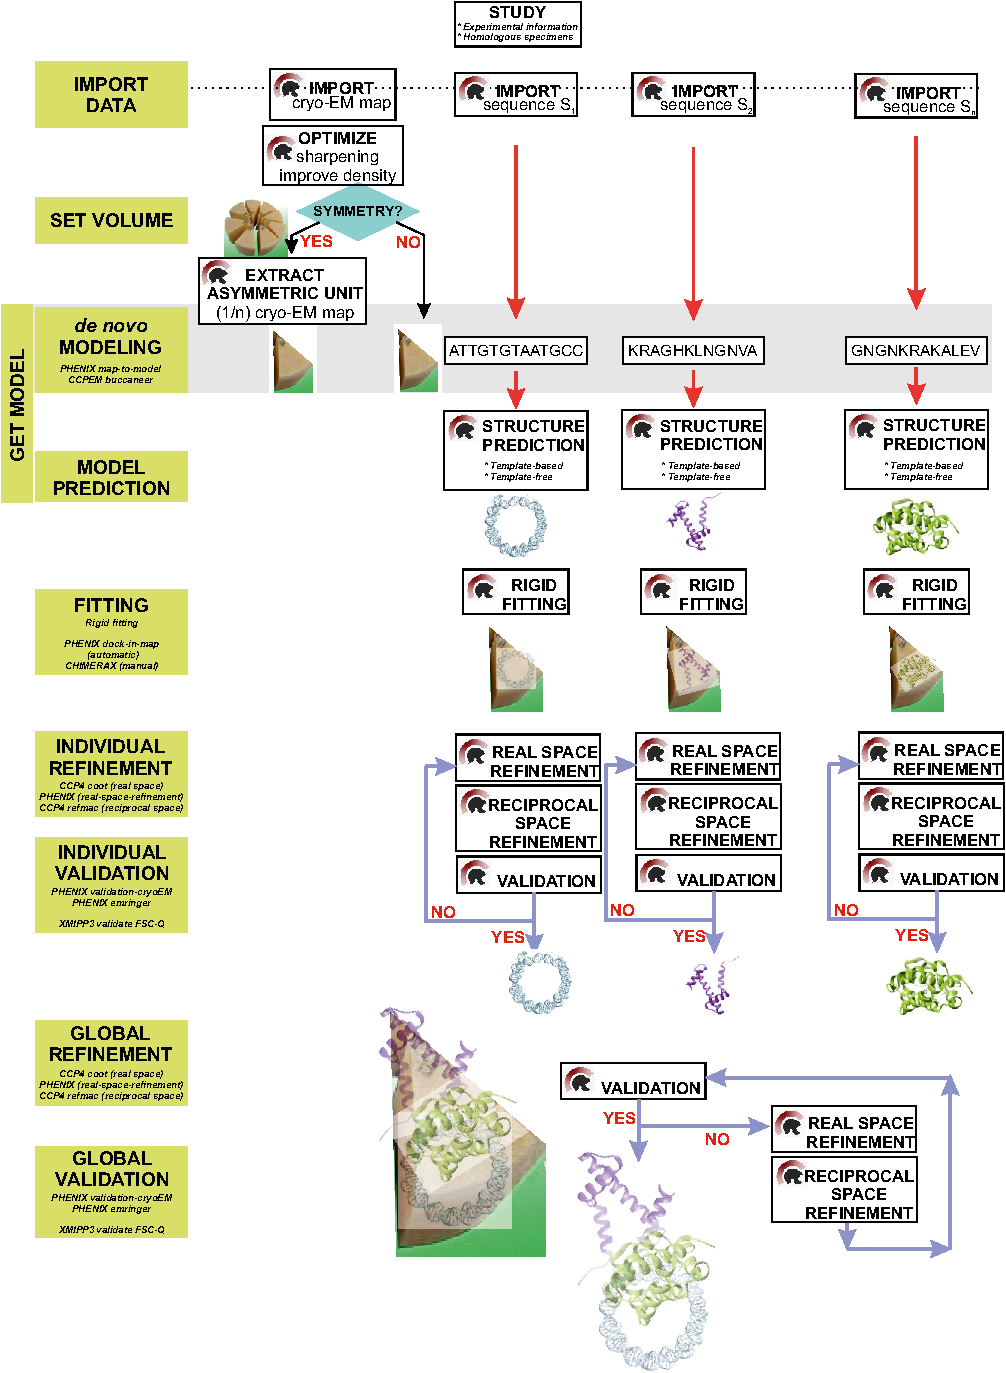
\includegraphics[width=0.95\textwidth]
  {{Images/Fig2.pdf}}
  \caption{General Model Building Workflow.}
  \label{fig:model_building_workflow}
  \end{figure} 
  


\section{Problem to solve: Apoferritin}

Ferritins are iron storage metalloproteins ubiquitously distributed among living organisms. These proteins are involved in iron metabolism in many different types of cells, and play a relevant dual role both in iron detoxification and iron reserve. The ferritin's architecture, similar to a spherical shell, is highly conserved in bacteria, plants and animals, and it allows to accumulate high amounts of Fe(III) atoms (up to 4000 per molecule). \\

The highly stable iron-free shell is known as apoferritin. Mammalian apoferritins are heteromeric molecules, constituted by 24 monomers structurally equivalent that surround the central cavity. Among these monomers, variable proportions of two types of subunits with different properties, H (heavy) and L (light), can be found. The tissues involved in iron storage contain higher proportion of L chains, whereas the tissues that require higher protection against oxidation, such as heart or brain, have a higher content of H chains. Unlike L chains, H chains display ferroxidase catalytic activity, necessary to oxidize Fe(II) to Fe(III). Concerning the structure of each subunit, it is constituted by 4 long helices, a fifth smaller helix and an additional extended loop. The dinuclear iron site, or ferroxidase site, is located in the center of the four helix bundle.\\

This tutorial will guide us in the building process of the mouse apoferritin 3D map using the \scipion framework (\ffigure{fig:workflow_pdf}). As starting input data, we are going to use the \ttt{EMPIAR ID: 10248} data, obtained from mouse heavy chain apoferritin. This cryo-EM data allowed to generate the 3D map \ttt{EMD-9865} at 1.54 \AA\ resolution \citep{hamaguchi2019}. The most recent atomic structure of mouse apoferritin, homo 24-mer of ferritin heavy chain with octahedral symmetry, was also obtained from cryo\-EM data at 1.84 \AA\ (\ttt{PDB ID: 6S61}). The 24 monomers of this metal binding protein are ligated to 6 Fe(III) and 24 Zn(II) ions.

\subsection*{Apoferritin processing workflow in \scipion}
\begin{figure}[H]
  \centering
  \captionsetup{width=.8\linewidth} 
  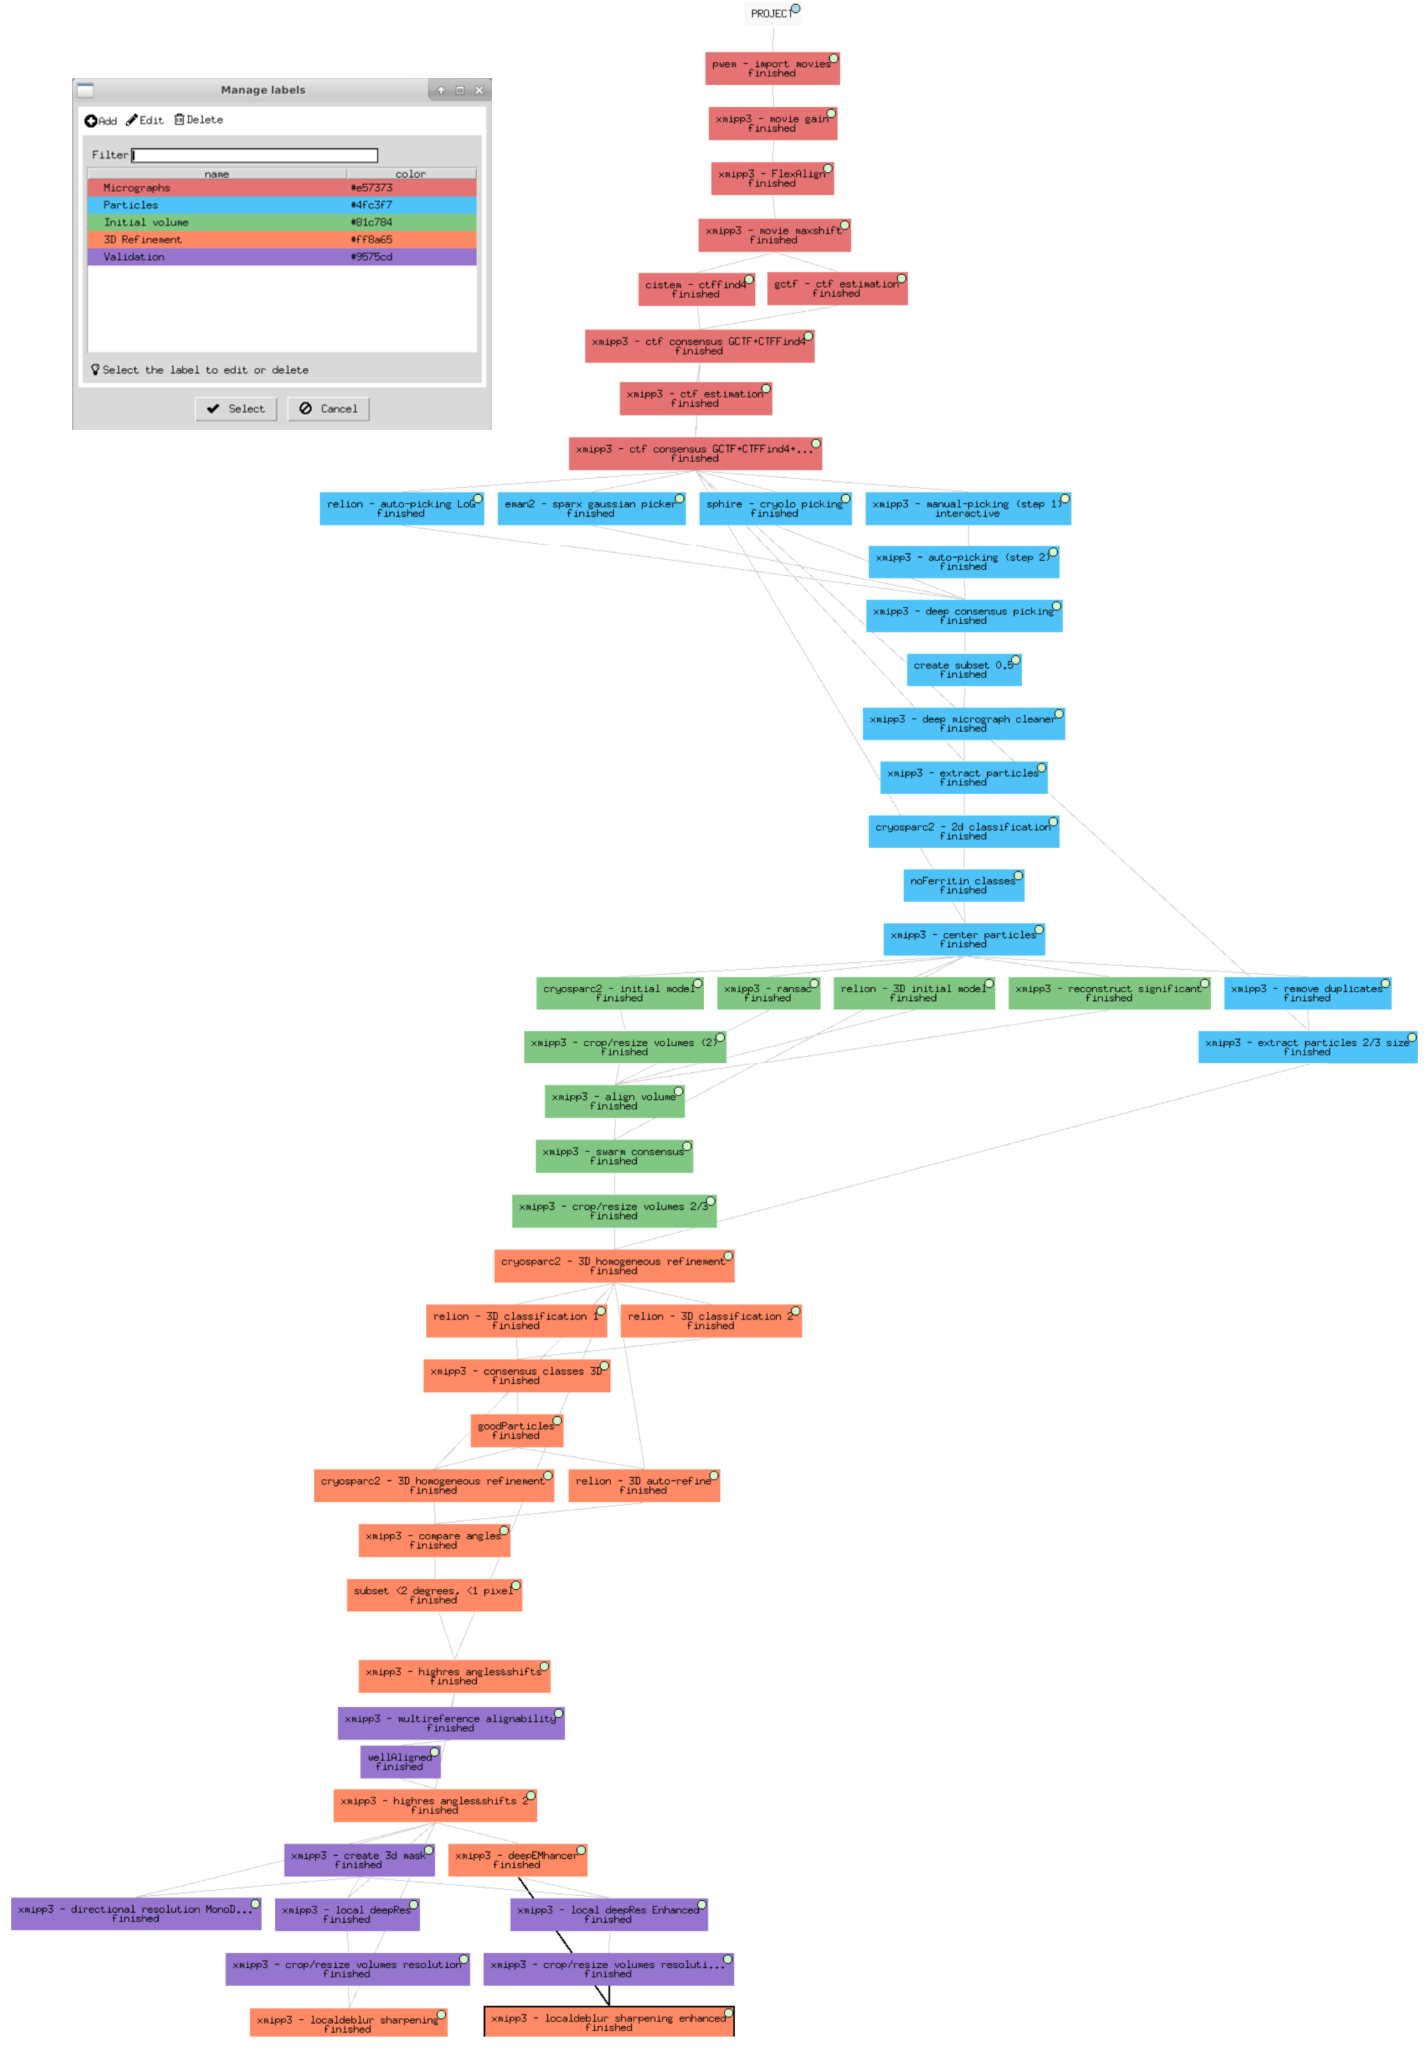
\includegraphics[width=0.95\textwidth]
  {images/workflow1.pdf}
  \caption{Apoferritin processing workflow.}
  \label{fig:workflow_pdf}
  \end{figure}







\section{Input data description}

 \subsection*{Map}
 Modeling means atomic interpretation of a map. This map can be the result of our own reconstruction process or can be obtained from a database. In this tutorial we use the haemoglobin map \ttt{EMD-3488}, that can be downloaded from \ttt{PDBE} (\url{http://www.ebi.ac.uk/pdbe/entry/emdb/EMD-3488}) (\ffigure{fig:PDBE}).\\
 WARNING in case you use your own map obtained from cryo-EM images: Take into account that cryo-EM 3D maps benefit significantly of an ``optimizing'' step, normally referred to as ``sharpening'' or ``density improvement``, that tends to increase signal at medium/high  resolution. Therefore, we recommend to sharp the map before tracing the atomic model. Either two \scipion protocols consecutively applied, \scommand{xmipp3 - local MonoRes} \citep{vilas2018} and \scommand{xmipp3 - localdeblur sharpening} \citep{ramirez2018}, or the protocol \scommand{xmipp3 - deepEMhancer} \citep{Sanchez-Garcia2020.06.12.148296}, allow map sharpening. Details about the parameters of these protocols are shown in Appendices \ref{app:localMonoRes}, \ref{app:localDeblurSharpening} and \ref{app:deepEMhancerSharpening}, respectively. 
 
 \begin{figure}[H]
  \centering
  \captionsetup{width=.8\linewidth} 
  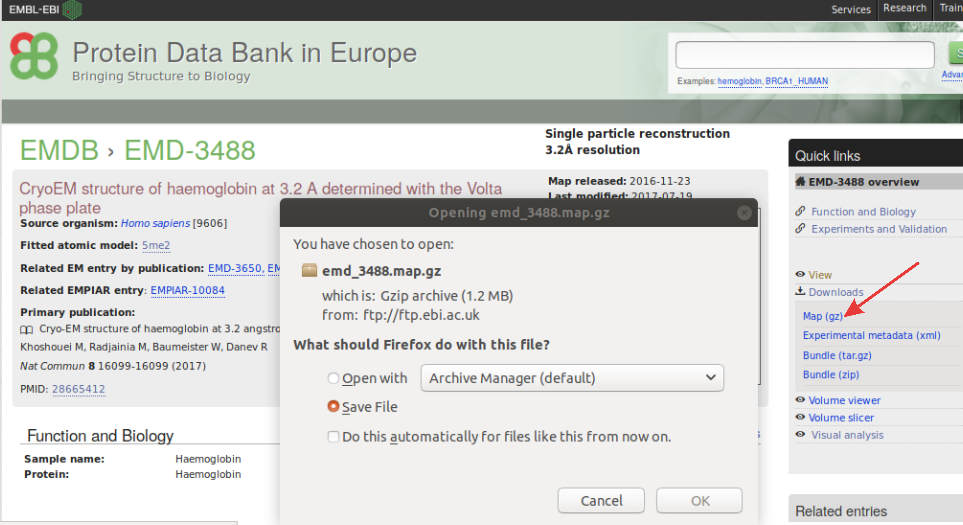
\includegraphics[width=0.95\textwidth]
  {{Images/Fig3}}
  \caption{Downloading the volume from \ttt{PDBe}.}
  \label{fig:PDBE}
  \end{figure}
  
  Once downloaded the volume, unpack it (command line: \ttt{gunzip emd-3488.map.gz}) and save it in your tutorial folder.
 
 \subsection*{Sequences}
 
 The sequences of \ttt{Hgb} $\alpha$ and $\beta$ subunits are included in \ttt{UniProtKB}. Accession numbers are \ttt{P69905} and \ttt{P68871}, respectively. Next, we show both sequences in fasta format:
 \begin{quote}
   \begin{verbatim}
>sp|P69905|HBA_HUMAN Haemoglobin subunit alpha
MVLSPADKTNVKAAWGKVGAHAGEYGAEALERMFLSFPTTKTYFPHFDLSHGSAQVKGHG
KKVADALTNAVAHVDDMPNALSALSDLHAHKLRVDPVNFKLLSHCLLVTLAAHLPAEFTP
AVHASLDKFLASVSTVLTSKYR

>sp|P68871|HBB_HUMAN Haemoglobin subunit beta
MVHLTPEEKSAVTALWGKVNVDEVGGEALGRLLVVYPWTQRFFESFGDLSTPDAVMGNPK
VKAHGKKVLGAFSDGLAHLDNLKGTFATLSELHCDKLHVDPENFRLLGNVLVCVLAHHFG
KEFTPPVQAAYQKVVAGVANALAHKYH
\end{verbatim}
 \end{quote}

 
 These protein sequences were determined by direct translation from the experimental sequence obtained from complementary \ttt{DNA (cDNA)}, i.e., \ttt{DNA} synthesized or retro-transcribed from messenger \ttt{RNA (mRNA)}. In this way, it is quite unlikely that these sequences include post-translational modifications. Although methionine is added with the translation \ttt{Met-tRNA} initiation factor, the removal of methionine aminoacid from the N-terminus of a polypeptide is a common post-translational modification. Since \ttt{Met} appears at the N-terminal end of both proteins, we can predict that these are not the polypeptide mature forms and \ttt{Met} will be removed in the mature ones that are present in the atomic structures. 
 
 Those two sequences can be retrieved from \ttt{UniProtKB} using \scipion\ \scommand{import sequence} protocol, which allows direct downloading from the database.
 


\section{Import Input data}
Taking advantage of \scipion software framework, we are going to import the above indicated input data using protocols \scommand{import volumes} and  \scommand{import sequence}. Details about the parameters of these two protocols are shown in Appendices \ref{app:importVolume} and \ref{app:importSequence}, respectively. 

 \begin{figure}[H]
  \centering 
  \captionsetup{width=.9\linewidth} 
  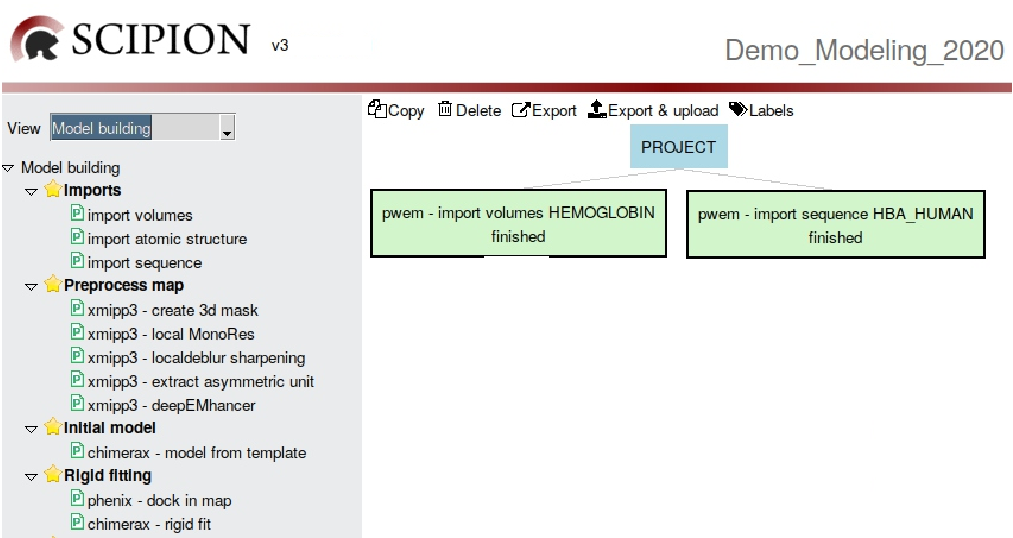
\includegraphics[width=0.95\textwidth]
  {Images/Fig61}
  \caption{\scipion framework with import workflow.}
  \label{fig:scipion_workflow_import_1}
  \end{figure}

(Note: The notation \ttt{Fig. X (a)} means that the step is shown in figure number X and there will be an arrow labeled with ``a'' marking the region of interest.)

 \subsection*{Volume}
 First open the \scommand{import volumes} protocol (\ffigure{fig:import_volume} (1)), fill in the form and execute it (2), and finally you may visualize the volume (3). 
 
 \begin{figure}[H]
  \centering 
  \captionsetup{width=.9\linewidth} 
  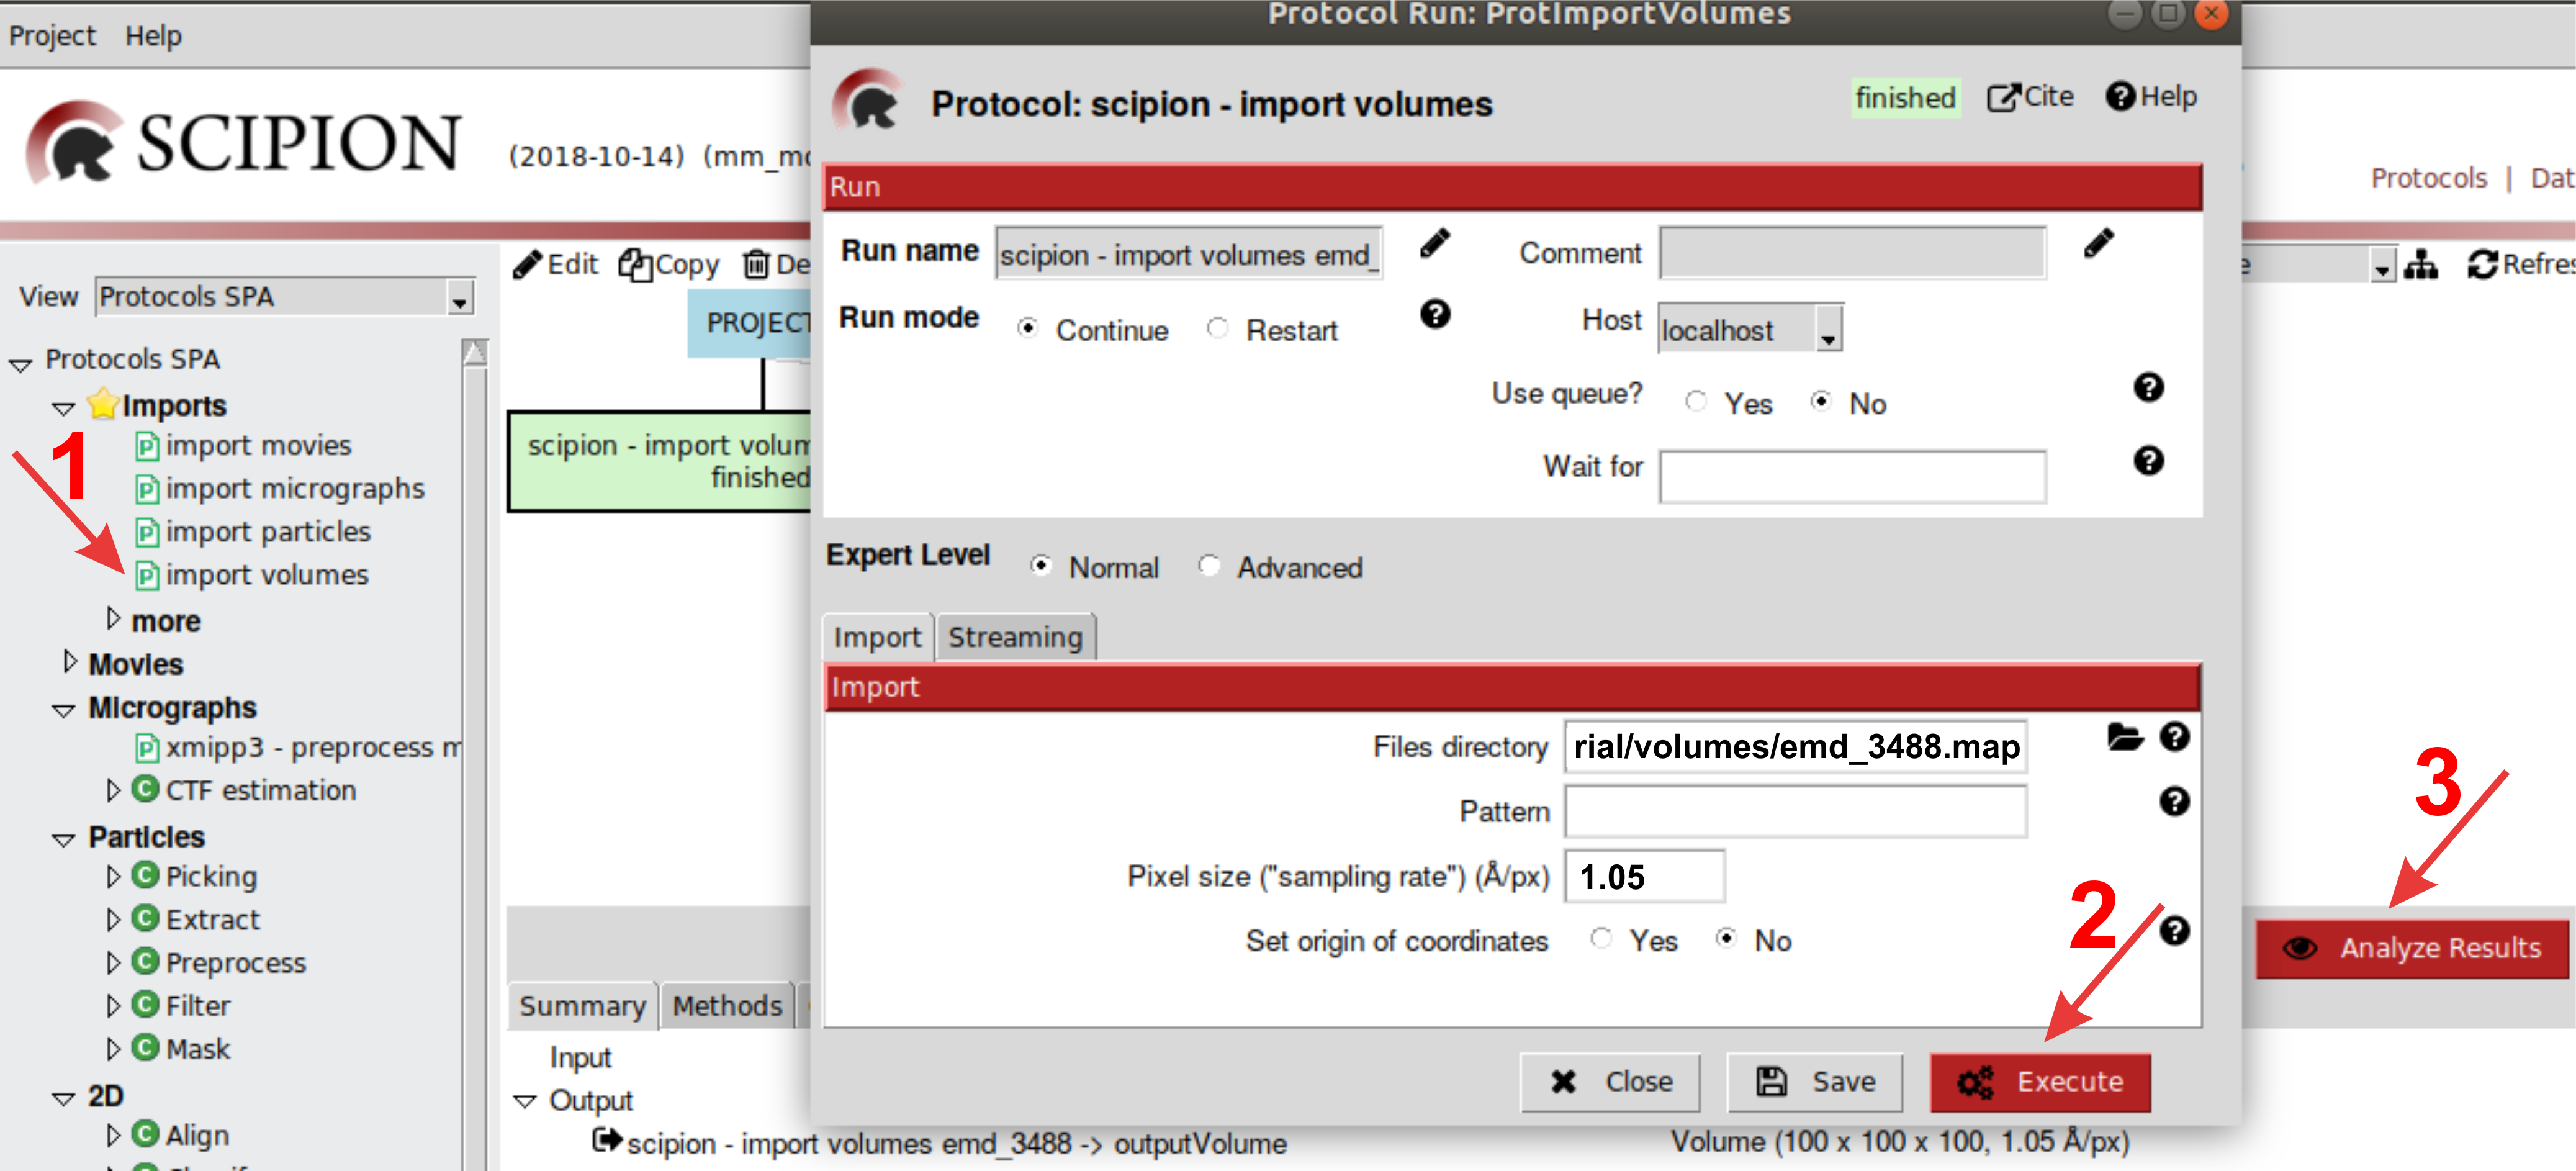
\includegraphics[width=0.95\textwidth]
  {Images/Fig4}
  \caption{Importing the volume in \scipion.}
  \label{fig:import_volume}
  \end{figure}
  
By default \chimera \citep{Goddard2018} is used for visualization. Clicking in the viewer menu  (\ffigure{fig:chimera_visualization_volume} (1)), \chimera shows the 3D map and the $x$ (red), $y$ (yellow) and $z$ (blue) axes.  
 %  The C2 symmetry is shown, as well as the 45º turn of volume regarding the z axis (blue line).
  
 \begin{figure}[H]
  \centering 
  \captionsetup{width=.9\linewidth} 
  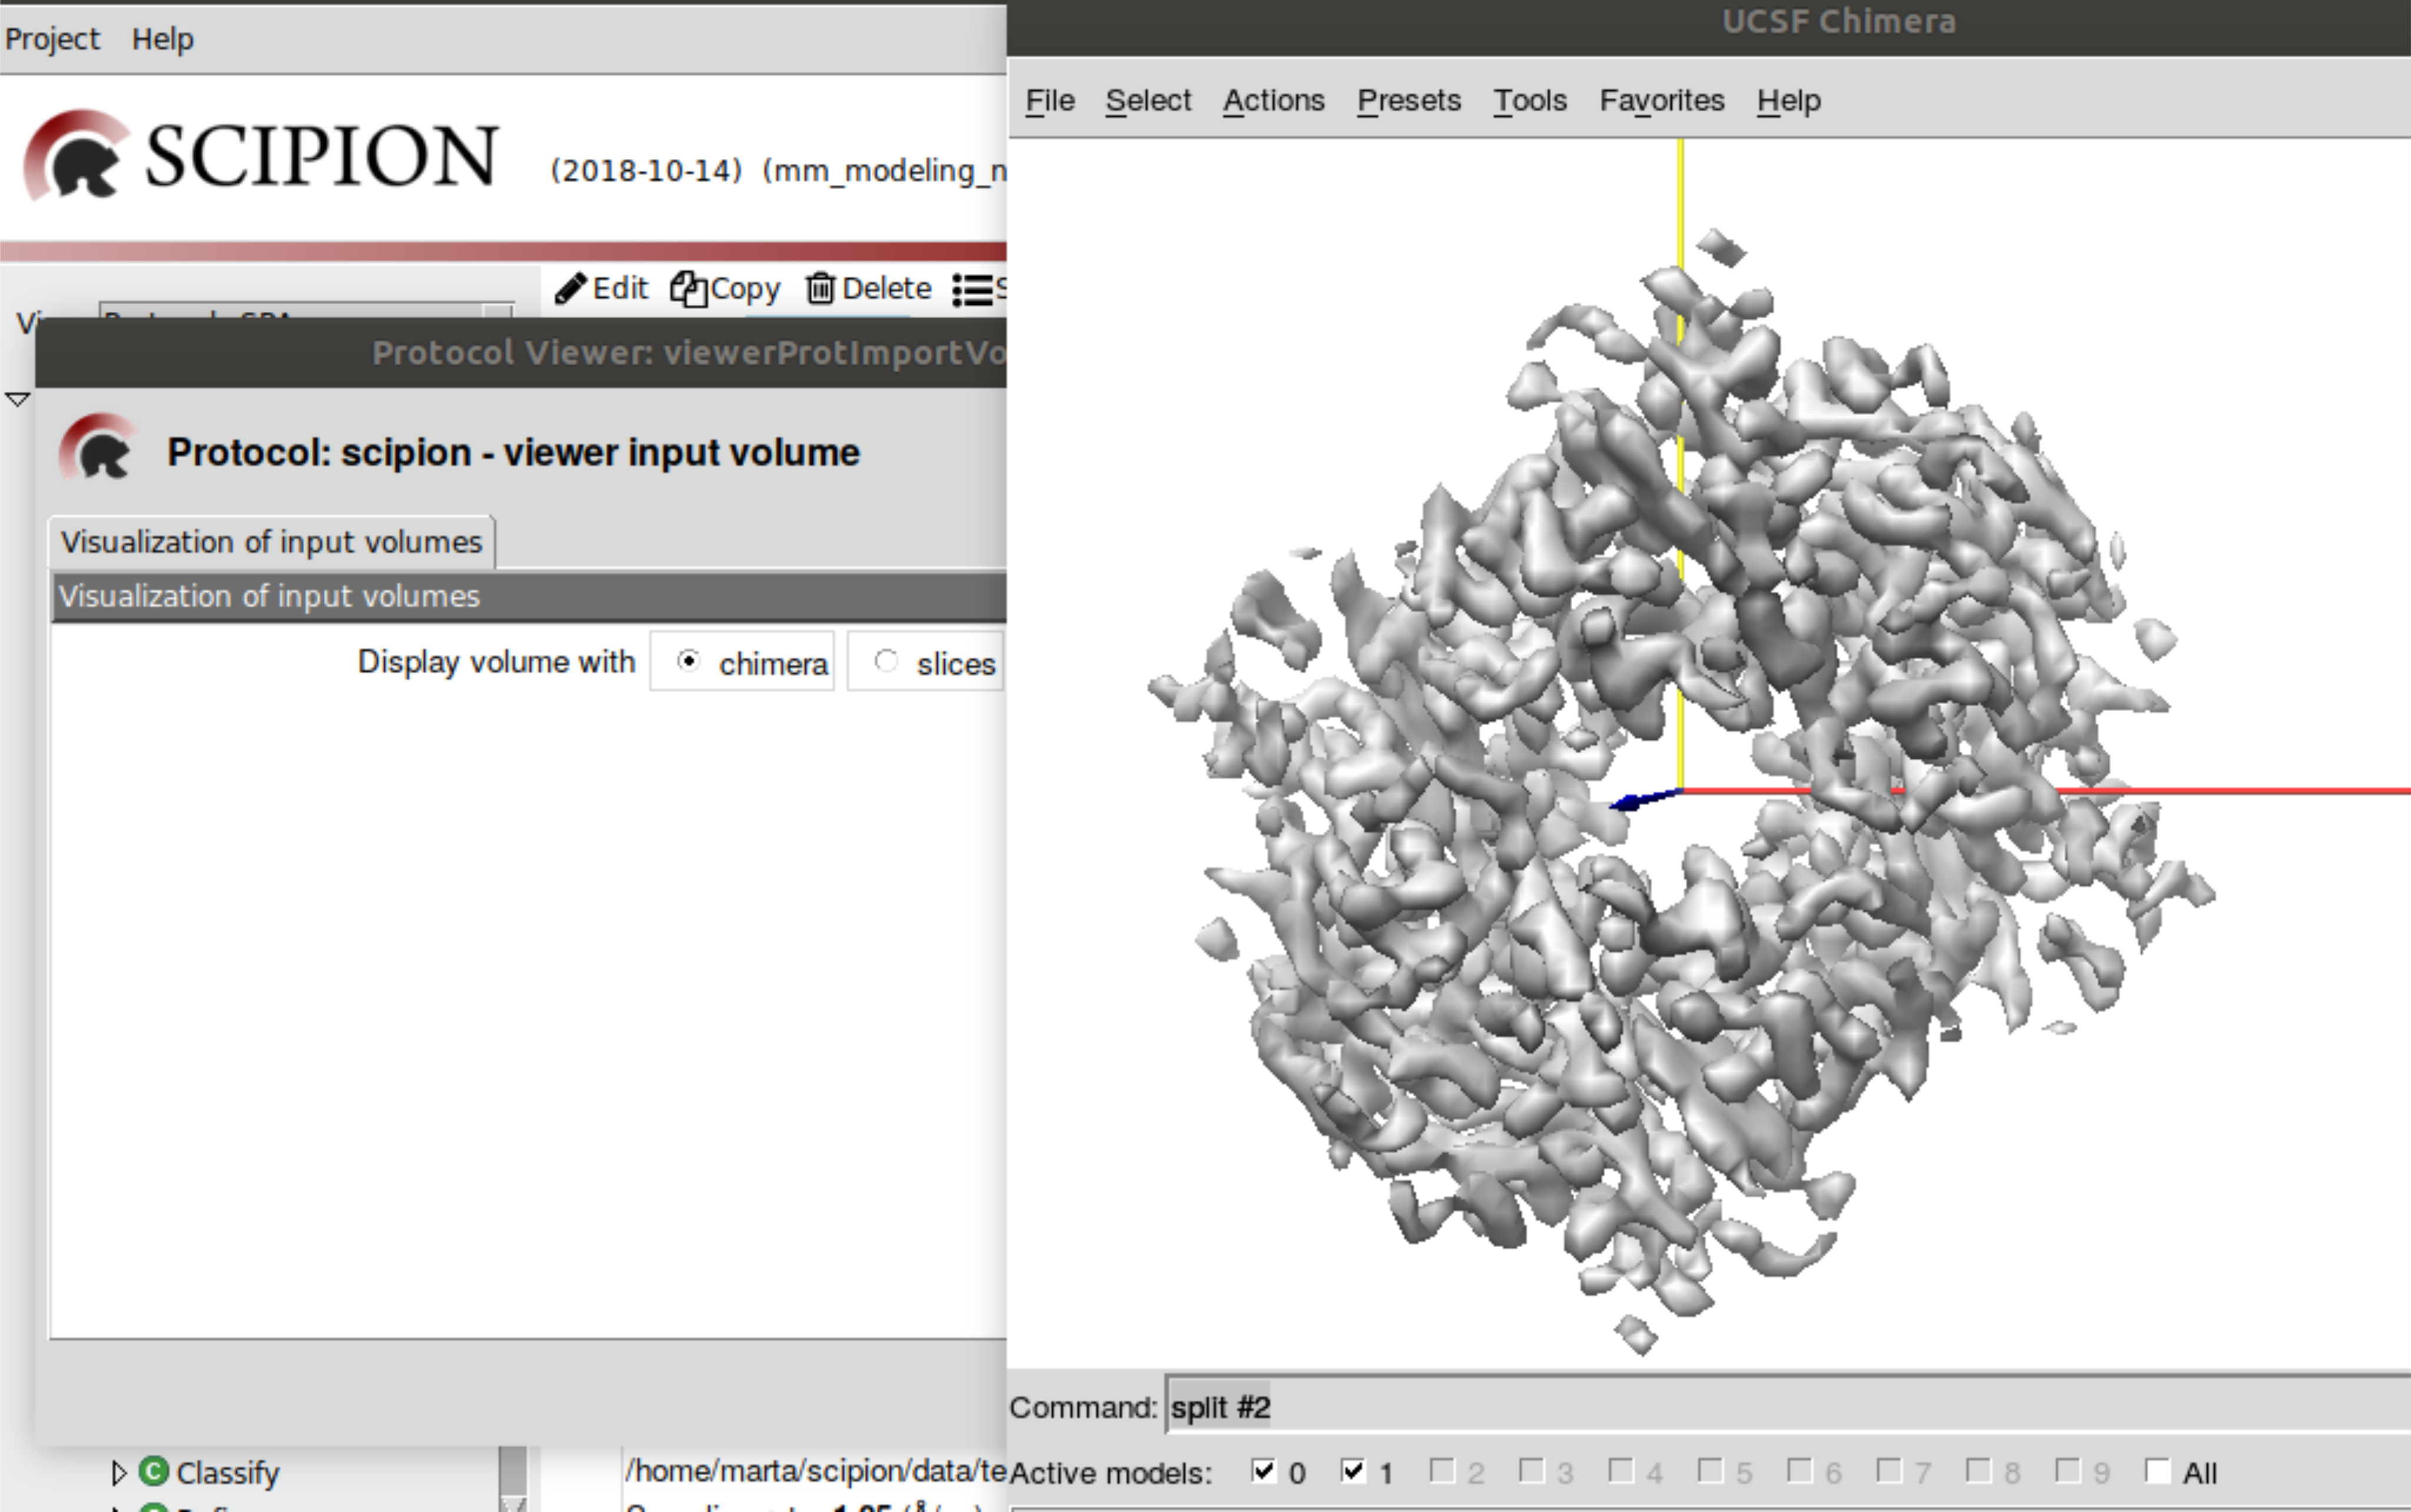
\includegraphics[width=0.95\textwidth]
  {Images/Fig5}
  \caption{Volume visualized with \chimera.}
  \label{fig:chimera_visualization_volume}
  \end{figure}
 
 \subsection*{Sequences}
 
 The sequences of \ttt{Hgb} $\alpha$ and $\beta$ subunits will be independently downloaded from \ttt{UniprotKB}. First of all, open the form of \scommand{import sequence} protocol (\ffigure{fig:import_sequence} (1)), then complete the form to download \ttt{HBA\_HUMAN} protein with \ttt{UniProtKB} accession code \ttt{P69905}, execute the process (2), and finally visualize the sequence (3) in a text editor. The sequence will appear in fasta format as it has been written above. Follow the same protocol to download \ttt{HBB\_HUMAN} with accession code \ttt{P68871}.
 
 \begin{figure}[H]
  \centering 
  \captionsetup{width=.9\linewidth} 
  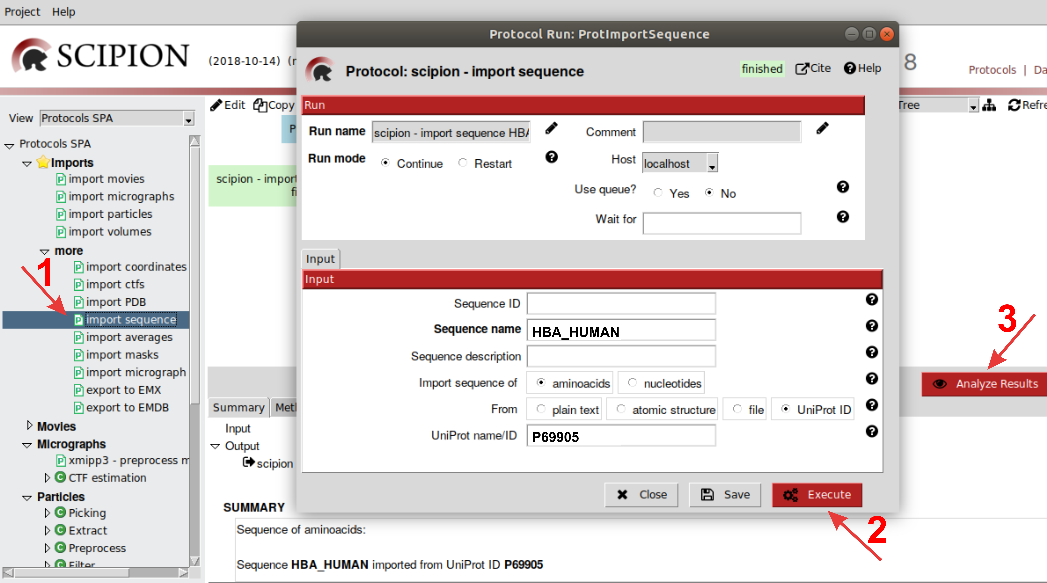
\includegraphics[width=0.95\textwidth]
  {Images/Fig6}
  \caption{Importing a \ttt{UniProtKB} sequence in \scipion.}
  \label{fig:import_sequence}
  \end{figure}
 

\section{3D Map preprocessing}
\ffigure{fig:scipion_workflow_import_2} shows the \scipion workflow that we are going to detail in this section.

 \begin{figure}[H]
  \centering 
  \captionsetup{width=.9\linewidth} 
  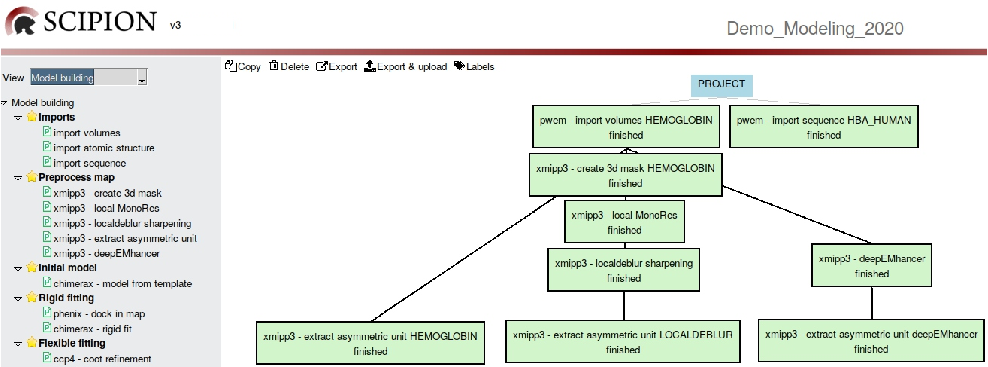
\includegraphics[width=0.95\textwidth]
  {Images/Fig62}
  \caption{\scipion framework detailing the workflow generated after 3D map preprocessing.}
  \label{fig:scipion_workflow_import_2}
  \end{figure}

\subsection*{Map sharpening}
As we have indicated before, since map sharpening contributes to increase signal at medium/high resolution, we recommend to perform this map preprocessing step before tracing the atomic model of cryo-EM 3D maps \citep{ramirez2018}.  To accomplish this task a couple of automatic alternatives are available in \scipion:  a) local sharpening method independent of initial model, based on local resolution estimation  (\scommand{xmipp3 - localdeblur sharpening} \citep{ramirez2018} (Appendix \ref{app:localDeblurSharpening})), b) deep learning-based sharpening approach (\scommand{xmipp3 - deepEMhancer} \citep{Sanchez-Garcia2020.06.12.148296} (Appendix \ref{app:deepEMhancerSharpening})). Although both sharpening methods display good results, these are not identical but complementary since $LocalDeblur$ maximizes specially details like the secondary structure, whereas $DeepEMhancer$ maximizes connectivity, favoring the fair tracing of the molecule skeleton.\\

Although the common first rule in both sharpening strategies is counting on half maps to get the best performance of the methods, or the average raw map otherwise, exceptionally in this case, to illustrate the procedure we are going to use the final postprocessed map deposited in the database, where no half maps have been submitted together with the final map.

\subsubsection*{a) Sharpening with $LocalDeblur$}
Since $LocalDeblur$ takes advantage of map local resolution to increase the signal, we have to compute this local resolution as first step to apply the $LocalDeblur$ sharpening method.  Although different algorithms could be used to compute local resolution, we have selected $MonoRes$ \citep{vilas2018}, implemented in \scipion in the protocol \scommand{xmipp3 - local MonoRes}  (Appendix \ref{app:localMonoRes}).\\ 
Since a map binary mask has optionally to be included as a parameter in this protocol, we will build a mask by using the \scipion protocol \scommand{xmipp3 - create 3d mask} (Appendix \ref{app:create3DMask}) as starting step in the local resolution estimation process. Open the protocol form (\ffigure{fig:create3Dmask_1} (1)) and fill in the tap \ttt{Mask generation} (2) with the input volume (3) and the density threshold (4). By default, the level value observed in \chimera main  graphics window (\ffigure{fig:chimera_visualization_volume}) \ttt{Tools -> Volume Data -> Volume Viewer -> Level} can be selected as threshold. In the \ttt{Postprocessing} tap (\ffigure{fig:create3Dmask_1} (5)), select \ttt{Yes} in \ttt{Apply morphological operation} (6) and maintain the rest of options by default. After executing this protocol (\ffigure{fig:create3Dmask_1} (7)), the morphology of the mask generated can be checked in slices by clicking \ttt{Analyze Results} (8).

 
 \begin{figure}[H]
  \centering 
  \captionsetup{width=.9\linewidth} 
  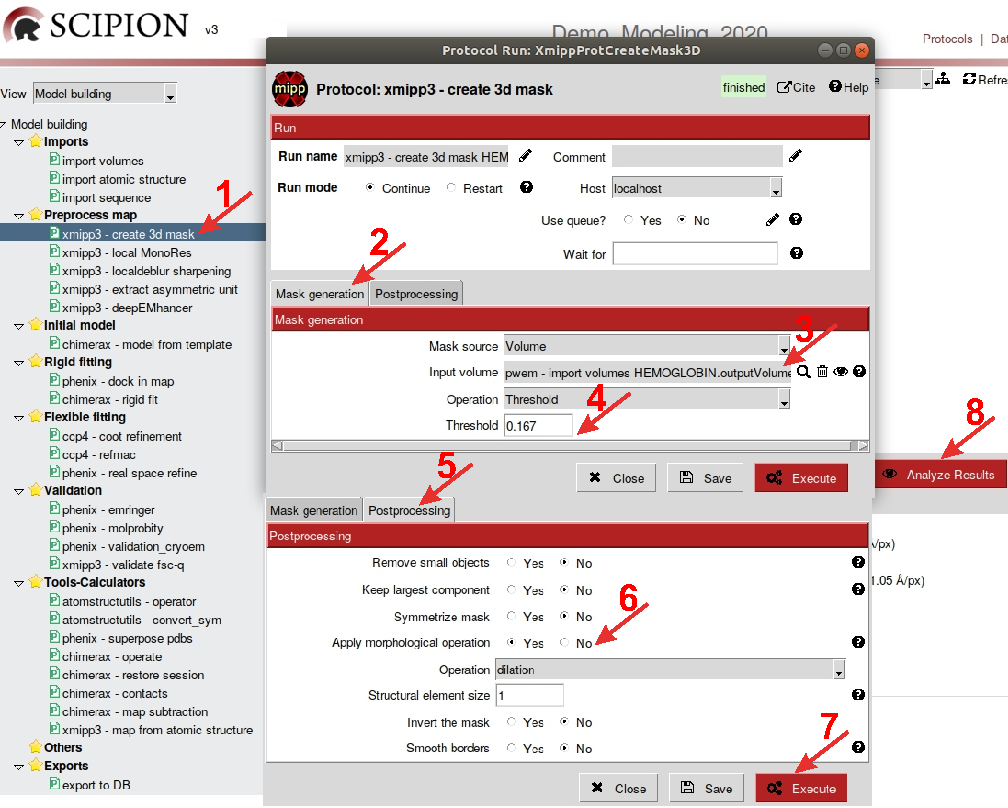
\includegraphics[width=0.95\textwidth]
  {Images/Fig53}
  \caption{Filling in the protocol to create a mask of the initial volume.}
  \label{fig:create3Dmask_1}
  \end{figure}
 
 $ShowJ$, the default \scipion viewer, allows visualize the mask with shape similar to the starting volume (\ffigure{fig:create3Dmask_2}).

 \begin{figure}[H]
  \centering 
  \captionsetup{width=.9\linewidth} 
  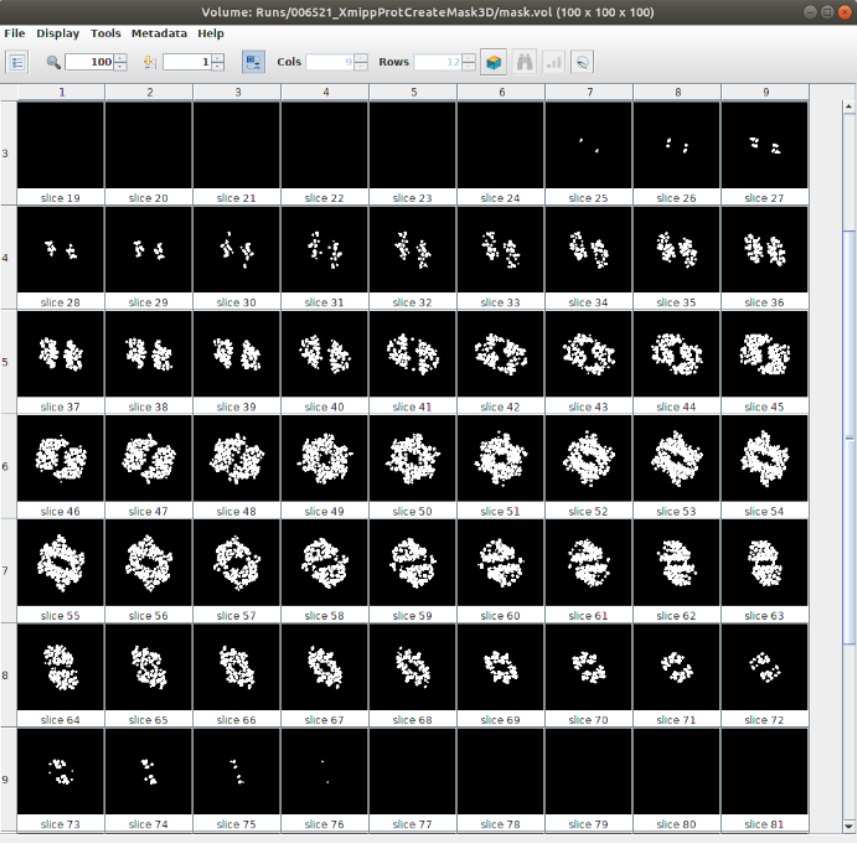
\includegraphics[width=0.60\textwidth]
  {Images/Fig54}
  \caption{Visualizing the mask of the initial volume.}
  \label{fig:create3Dmask_2}
  \end{figure}
  
\ttt{NOTE}: In case you would like to use a previous computed mask, you can do it simply by importing it using the protocol \scommand{import mask} (Appendix \ref{app:importMask}).\\
  
Once the mask of the starting map has been created, the protocol of \scommand{xmipp3 - local MonoRes} can be completed to get the estimation of local resolution. Open the protocol (\ffigure{fig:localMonoRes_1} (1)) and include the starting map (2), as well as the binary mask (3). Finally, based on the map resolution (3.2 \AA), select the default resolution range between \ttt{0.0} and \ttt{6.0} \AA (4). 

\begin{figure}[H]
  \centering 
  \captionsetup{width=.9\linewidth} 
  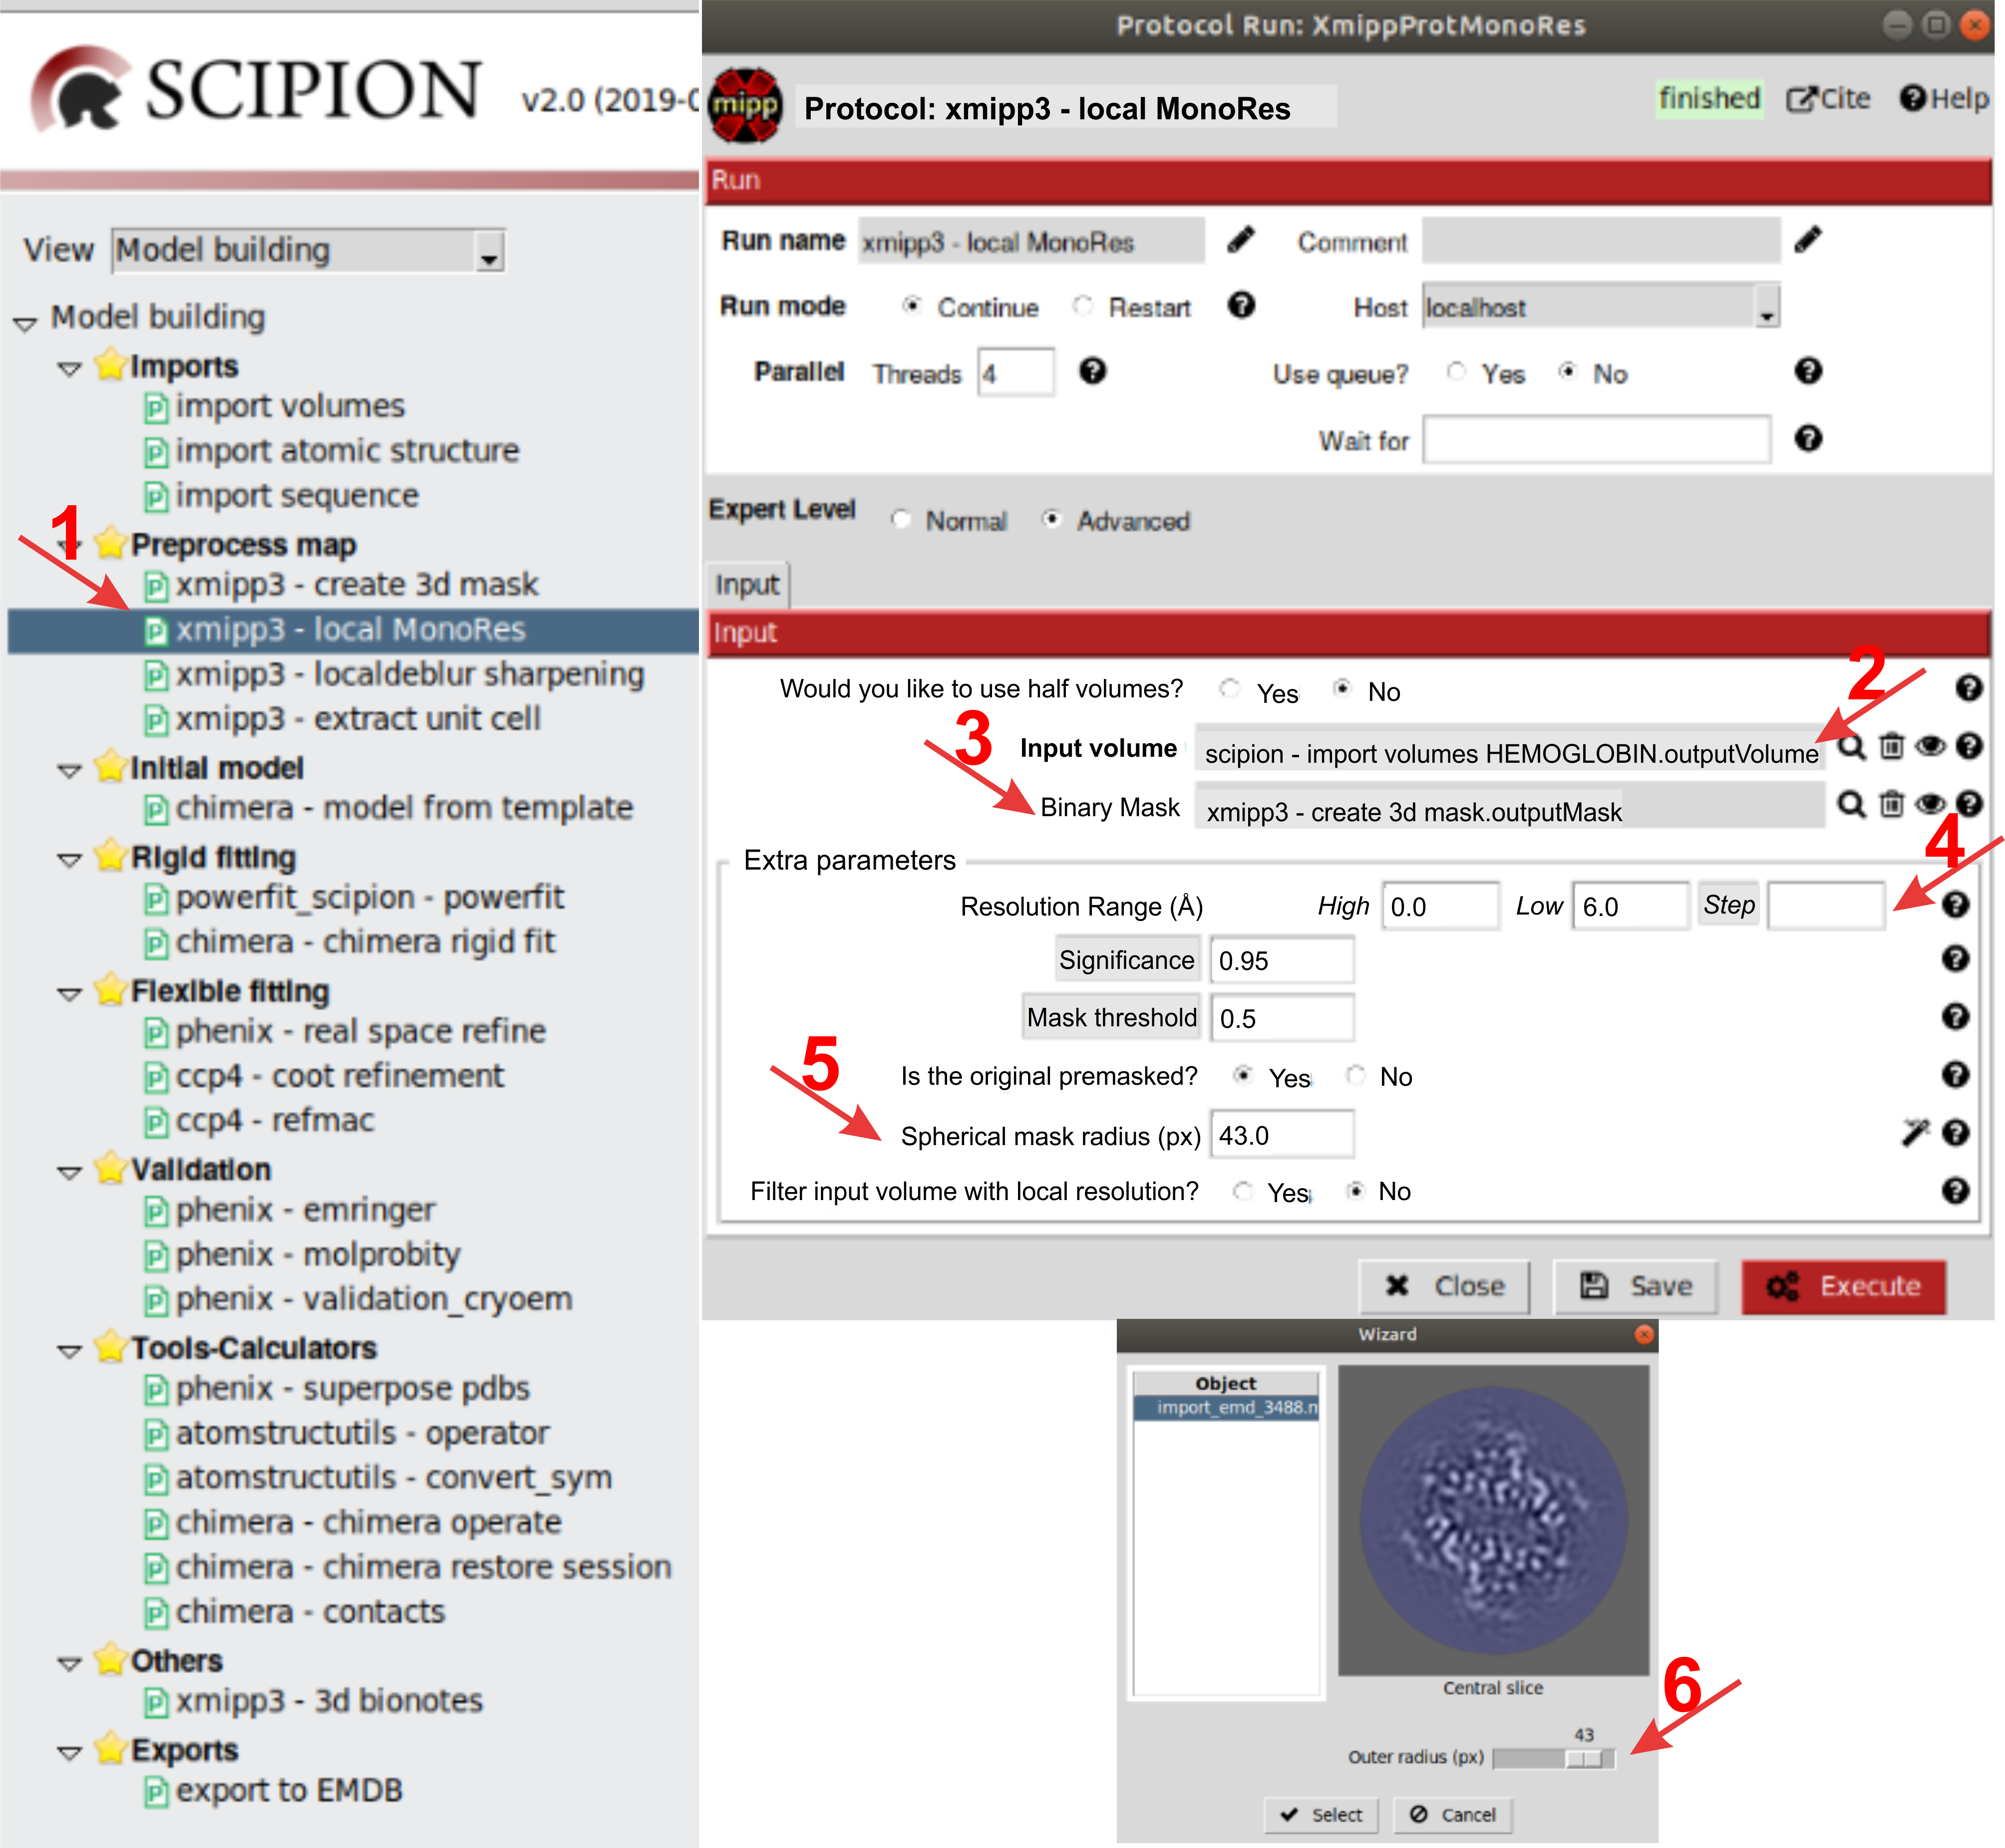
\includegraphics[width=1\textwidth]
  {Images/Fig55}
  \caption{Completing the protocol to estimate the local resolution of the \ttt{metHgb} map.}
  \label{fig:localMonoRes_1}
  \end{figure}
  
Execute this protocol (\ffigure{fig:localMonoRes_1} (5)) and analyze the results (6). The menu of results (\ffigure{fig:localMonoRes_2} (A)), among other views, shows the histogram of local resolutions (1) and the resolution map in \chimera (2). The histogram of resolutions, which displays the number of map voxels showing a certain resolution, allows to conclude that the majority of voxels evidence a resolution between 3.2 and 3.5 \AA, quite close to the published map resolution (3.2 \AA).The resolution map shown by \chimera details the resolution of each voxel (\ffigure{fig:localMonoRes_3}). The bar on the left indicates the color code for resolution values.

\begin{figure}[H]
  \centering 
  \captionsetup{width=.9\linewidth} 
  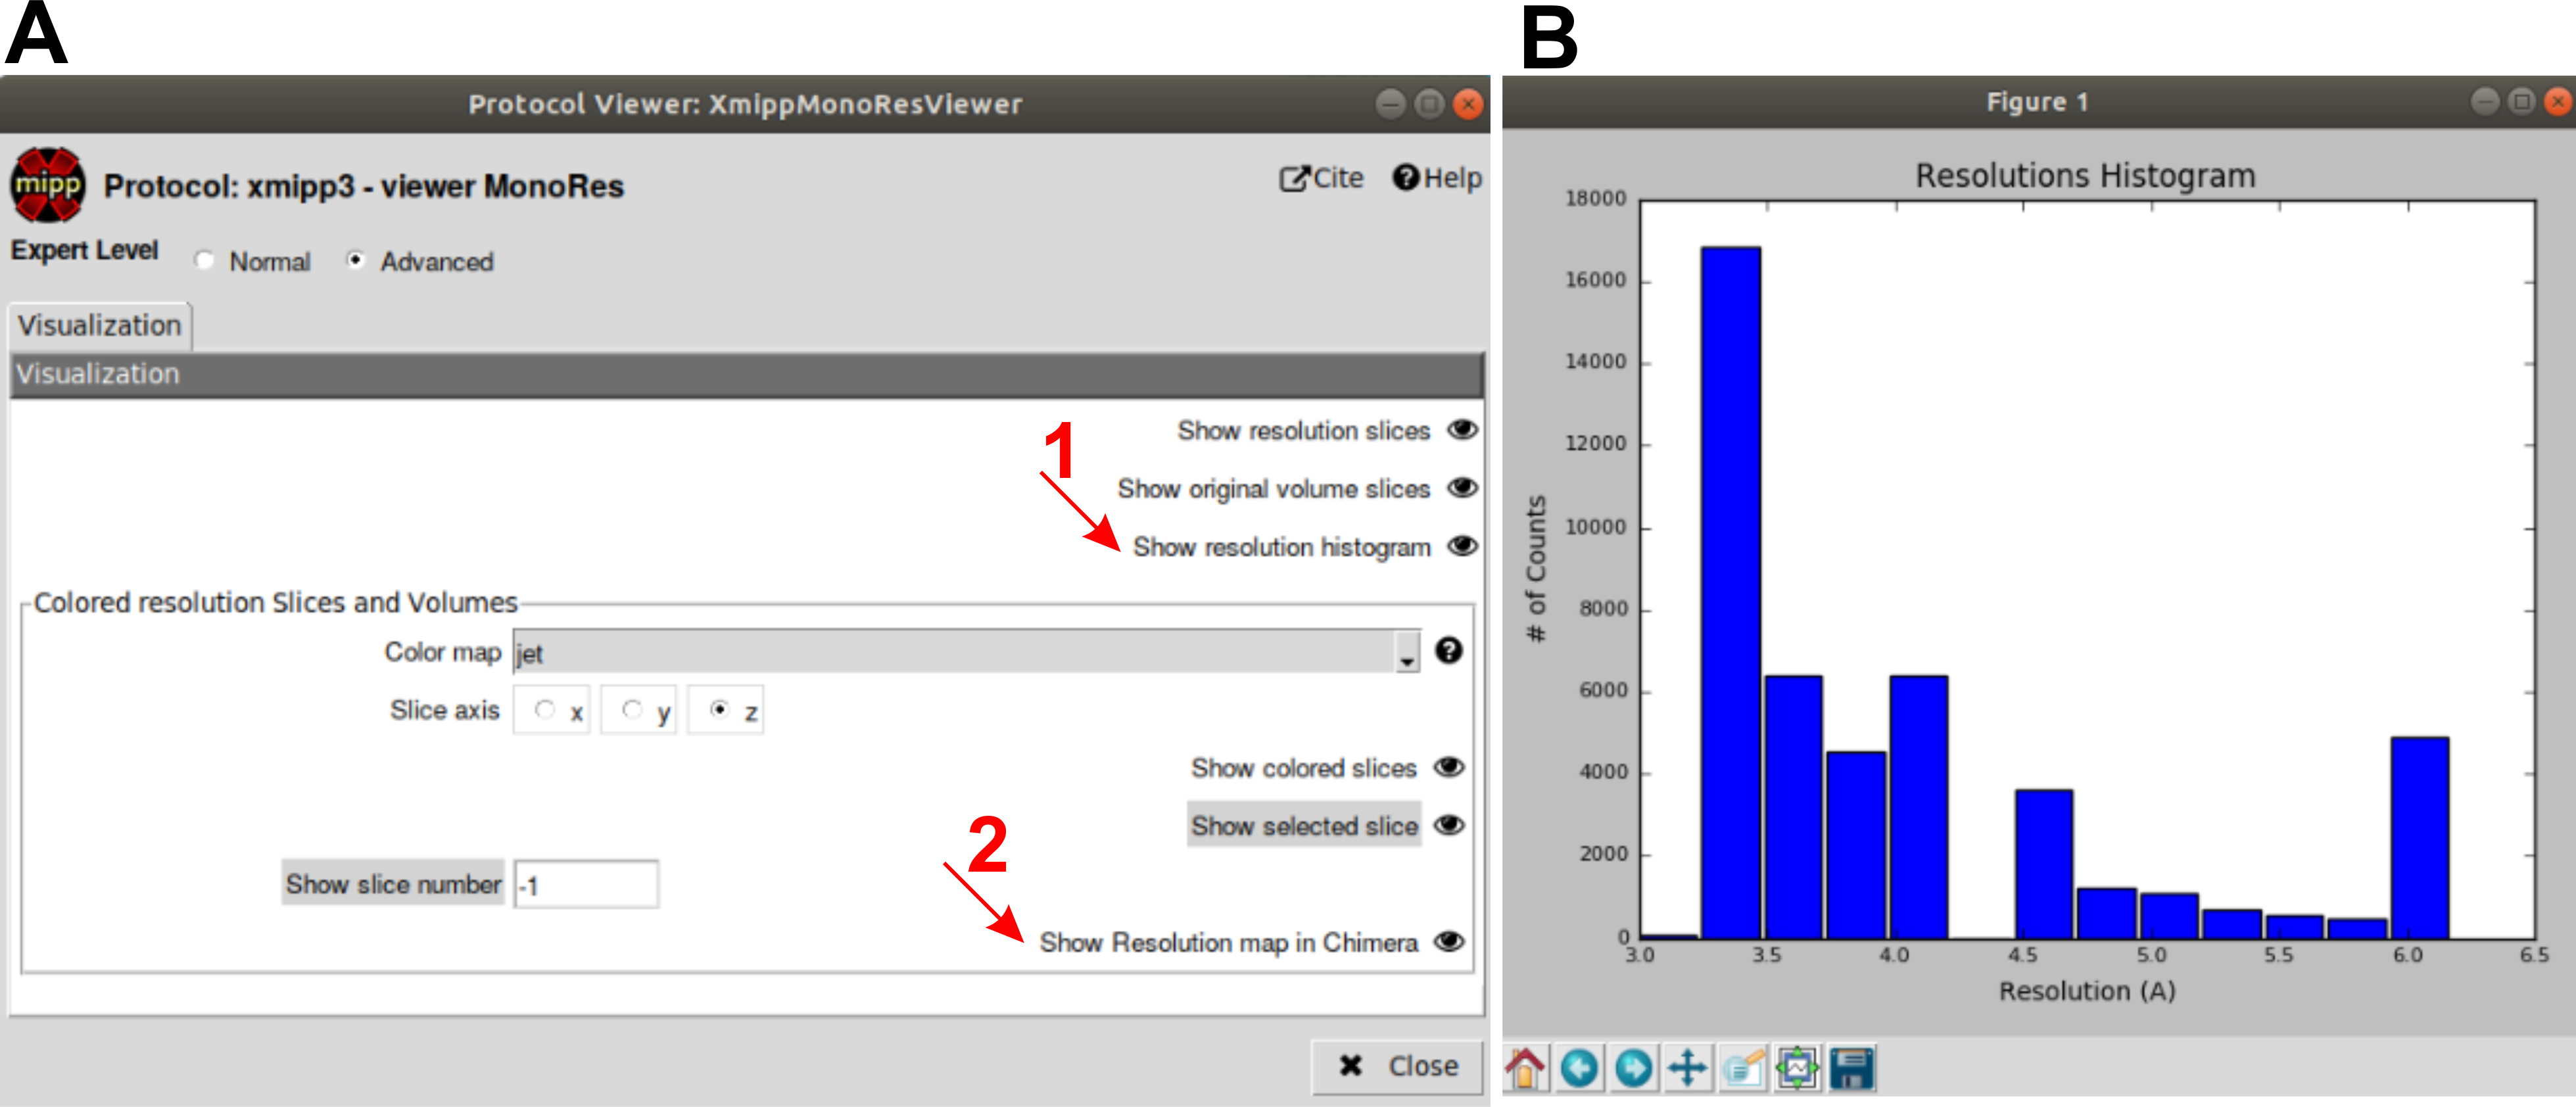
\includegraphics[width=0.80\textwidth]
  {Images/Fig56}
  \caption{\scommand{xmipp3 - local MonoRes} menu of results (A) and histogram of resolutions (B).}
  \label{fig:localMonoRes_2}
  \end{figure}
  
\begin{figure}[H]
  \centering 
  \captionsetup{width=.7\linewidth} 
  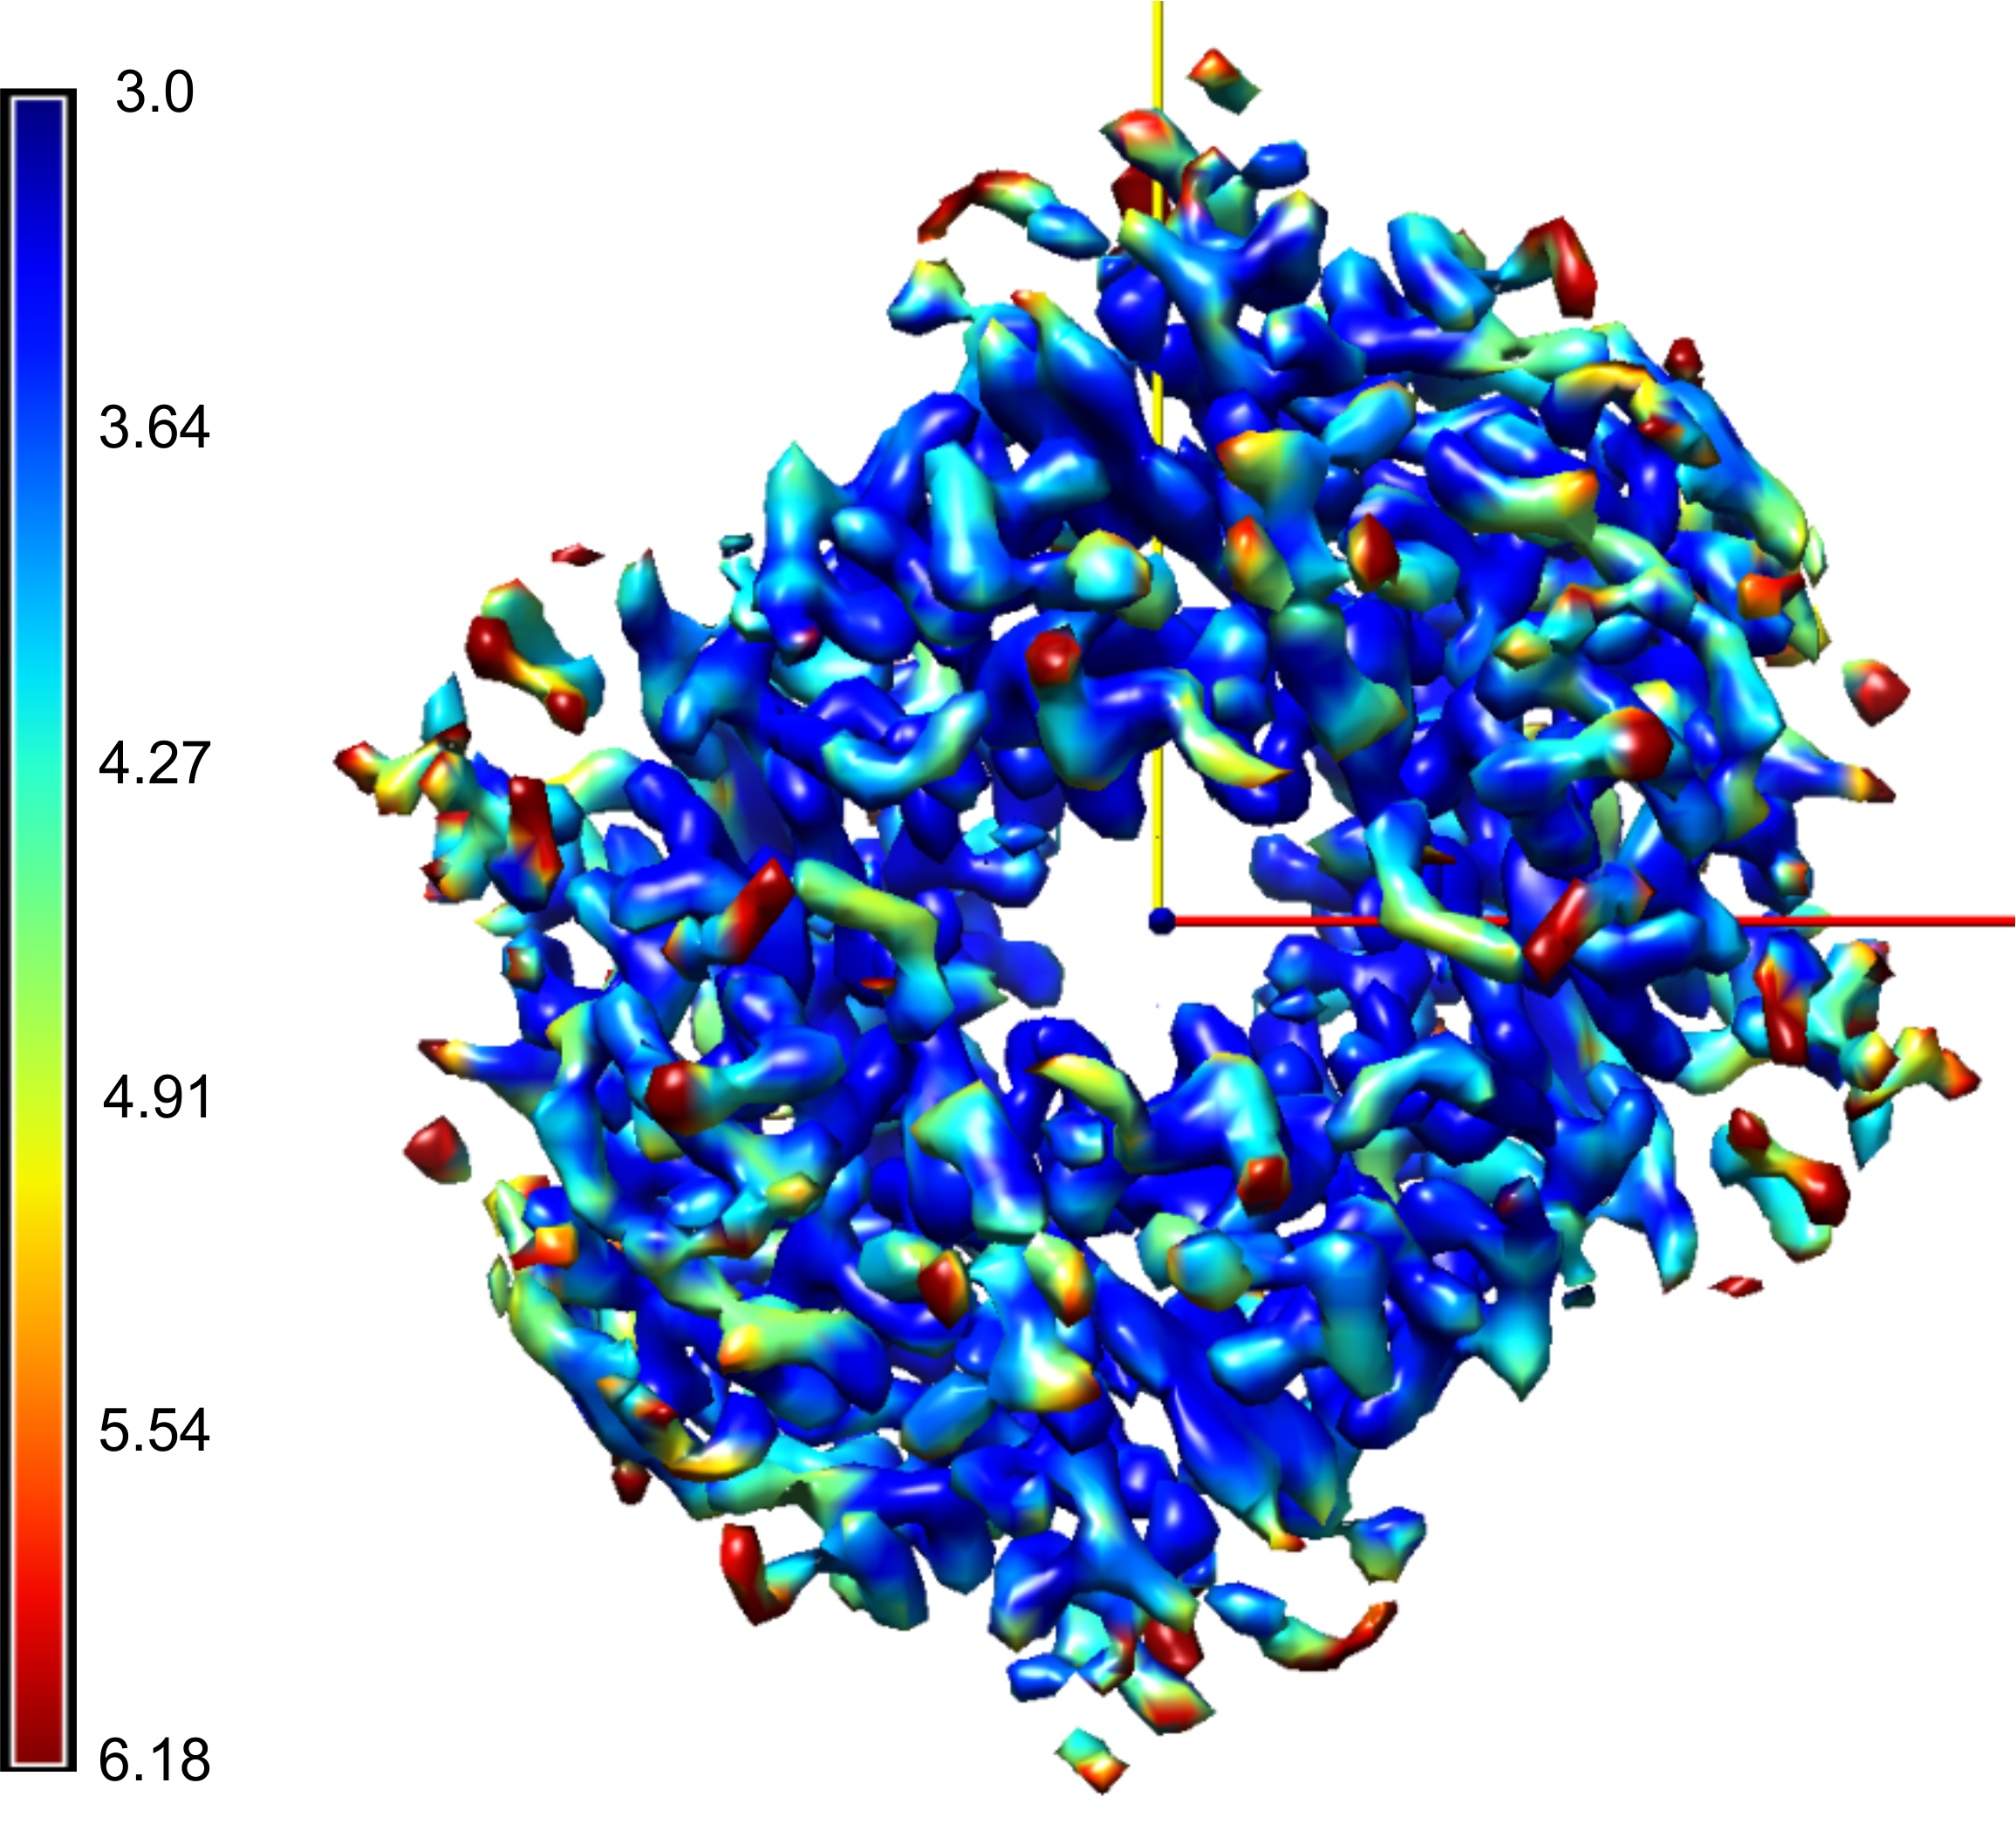
\includegraphics[width=0.70\textwidth]
  {Images/Fig57}
  \caption{Resolution map in \chimera.}
  \label{fig:localMonoRes_3}
  \end{figure}
  
Local resolution values of the input map allow to compute the sharpened map by the \scommand{xmipp3 - localdeblur sharpening} protocol, which implements an iterative steep descending method that not requires initial model. To accomplish this step, open the protocol (\ffigure{fig:localdeblur_1} (1)) and include the starting map (2) and the map of resolution values (3), maintaining the default values for the rest of parameters (4, 5). 

\begin{figure}[H]
  \centering 
  \captionsetup{width=.9\linewidth} 
  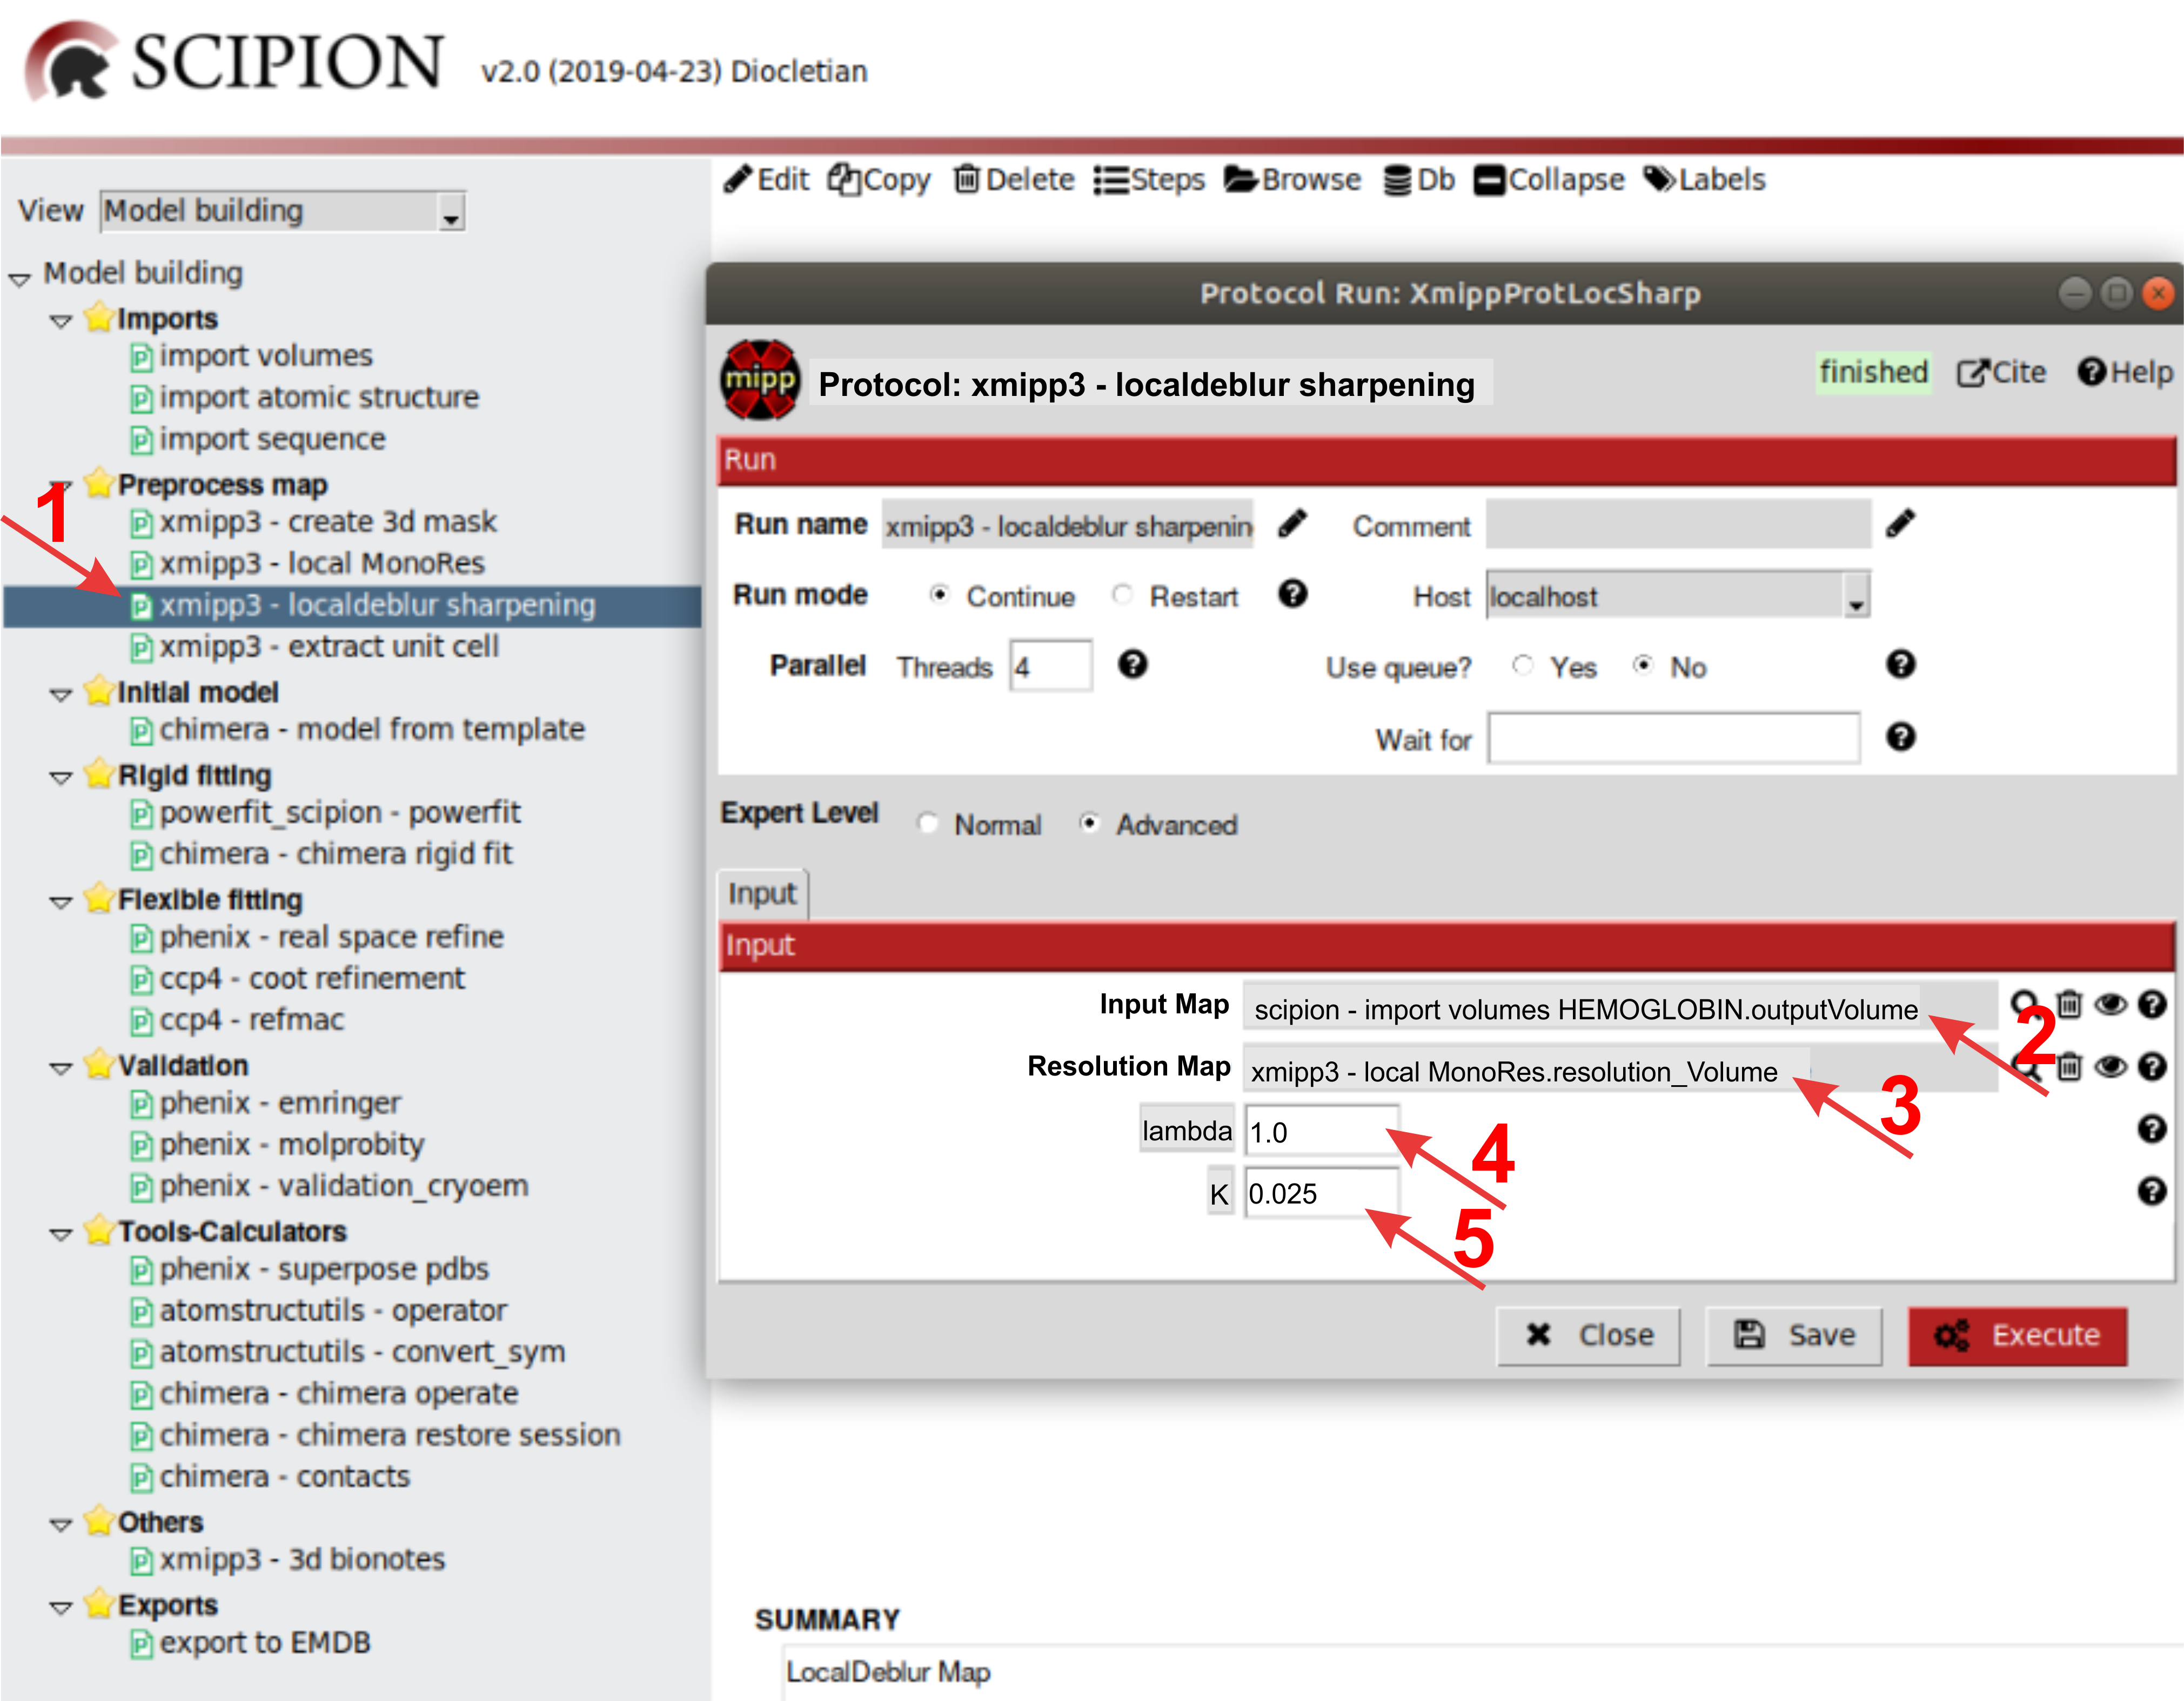
\includegraphics[width=1\textwidth]
  {Images/Fig58}
  \caption{Filling in the protocol to compute the sharpened map.}
  \label{fig:localdeblur_1}
  \end{figure}
  
After two iterations, the sharpening algorithm reached the convergence criterion, $i.e.$ a difference between two successive iterations lower than 1 \%, and stopped. The two maps obtained in the respective iterations can be observed with $ShowJ$ by clicking the black arrow shown in \ffigure{fig:localdeblur_1} (7) with the right mouse botton and selecting \ttt{Open with DataViewer}. Resulting map for each iteration will be shown, as indicated in \ffigure{fig:localdeblur_2}.  Visualization in \chimera is also possible selecting \ttt{Open with ChimeraX} in the menu option \ttt{File} (\ffigure{fig:localdeblur_2} (1)). 

\begin{figure}[H]
  \centering 
  \captionsetup{width=.9\linewidth} 
  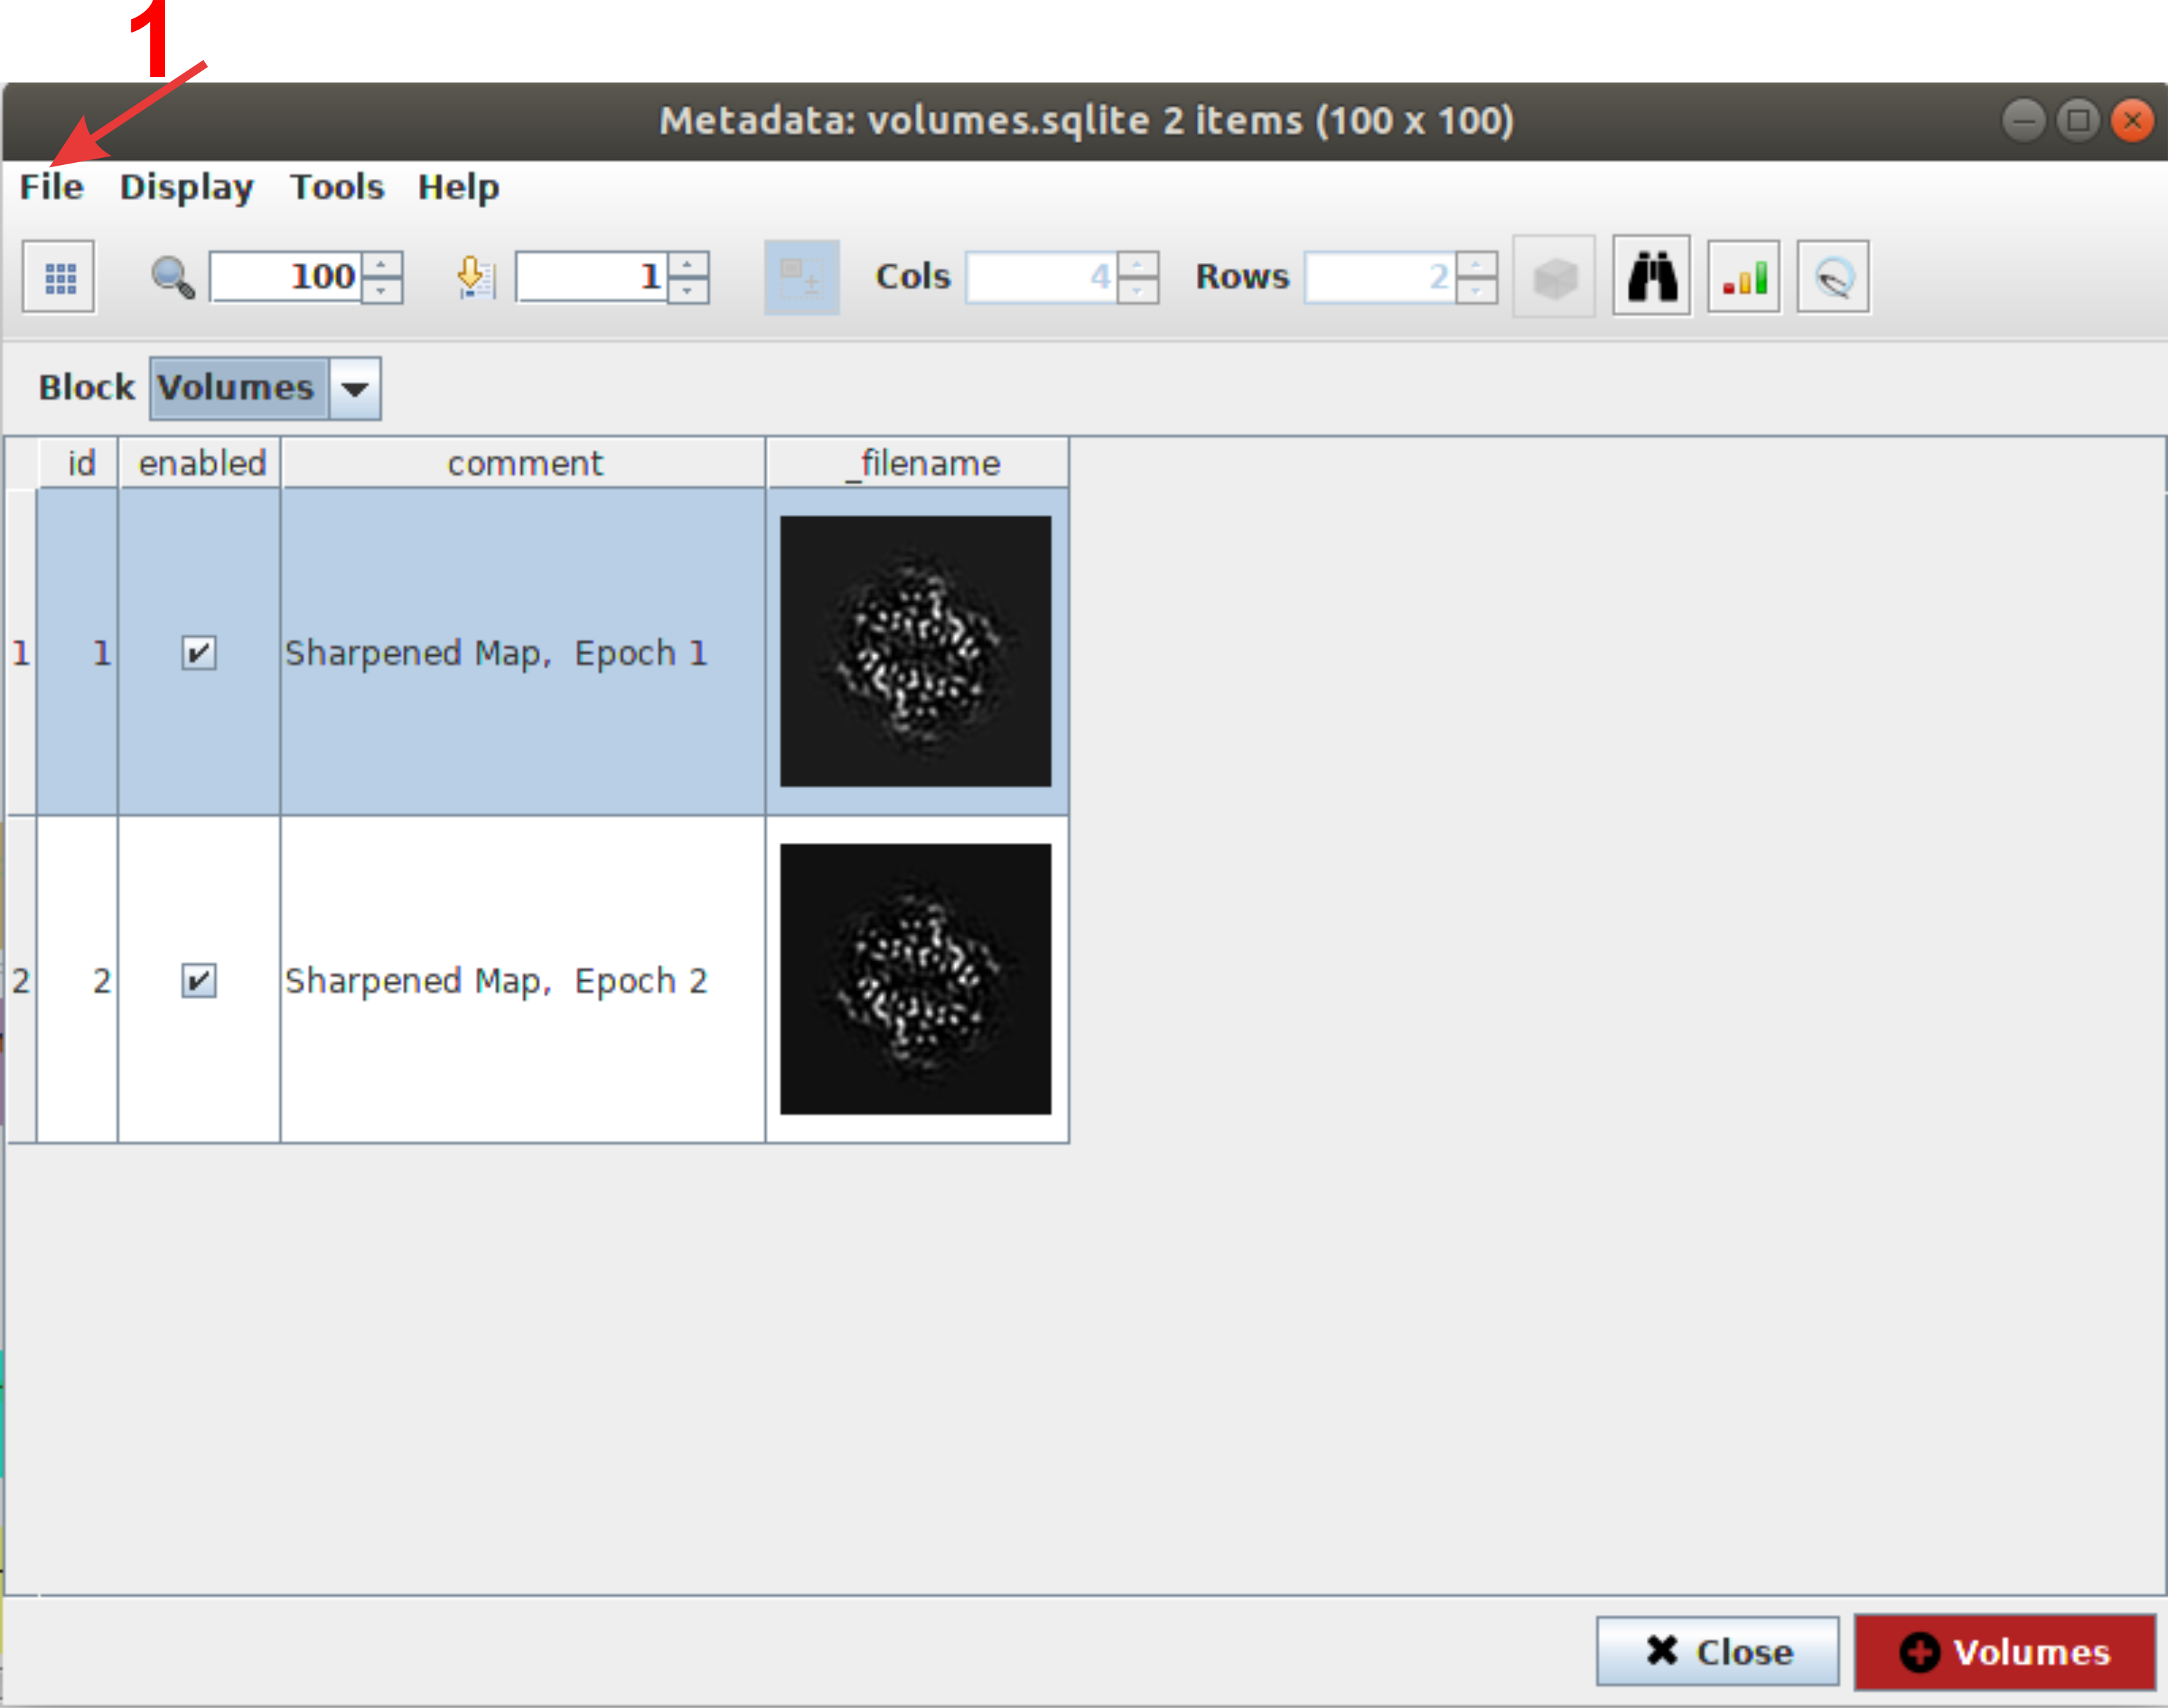
\includegraphics[width=0.65\textwidth]
  {Images/Fig59}
  \caption{Sharpened maps generated after two iterations.}
  \label{fig:localdeblur_2}
  \end{figure}
  
Additionally, by clicking \ttt{Analyze Results} (\ffigure{fig:localdeblur_1} (6)) the sharpened map obtained after the second iteration, $i.e.$ the \ttt{last} map, can be also visualized and compared with the initial one in \chimera (\ffigure{fig:localdeblur_3}).


\begin{figure}[H]
  \centering 
  \captionsetup{width=.9\linewidth} 
  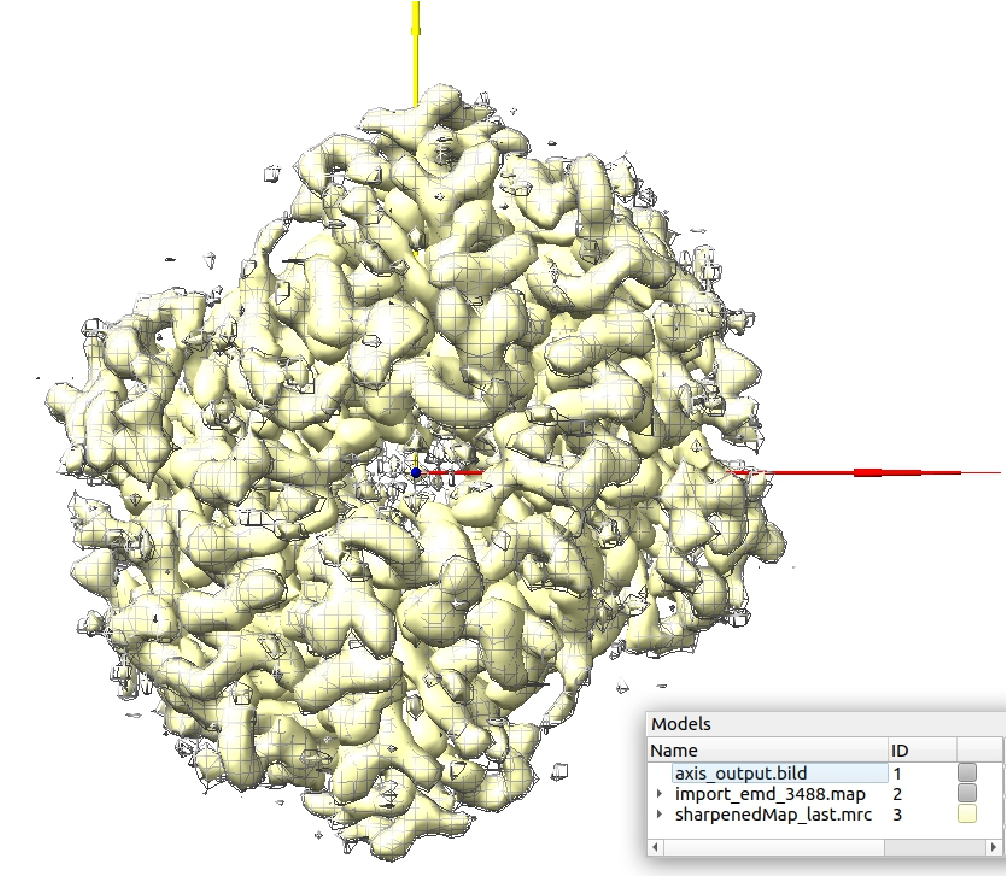
\includegraphics[width=0.65\textwidth]
  {Images/Fig64}
  \caption{$LocalDeblur$ \ttt{last} iteration sharpened map (yellow surface) and input map (grey mesh) in \chimera.}
  \label{fig:localdeblur_3}
  \end{figure}
 
\subsubsection*{b) Sharpening with $DeepEMhancer$}

$DeepEMhancer$ is an alternative automatic sharpening method based on deep learning (\citep{Sanchez-Garcia2020.06.12.148296}), implemented in \scipion in the protocol \scommand{xmipp3 - deepEMhancer} (Appendix \ref{app:deepEMhancerSharpening}). Open this protocol (\ffigure{fig:deepEMHancer_1} (1)) and complete it as indicated. Since only the refined map is available, we are not going to use half maps (2). Include your map (3), the type of normalization desired (4) and the deep learning mode to use (5), in this particular case \ttt{highRes} due to the map high resolution.

 
 \begin{figure}[H]
  \centering 
  \captionsetup{width=.9\linewidth} 
  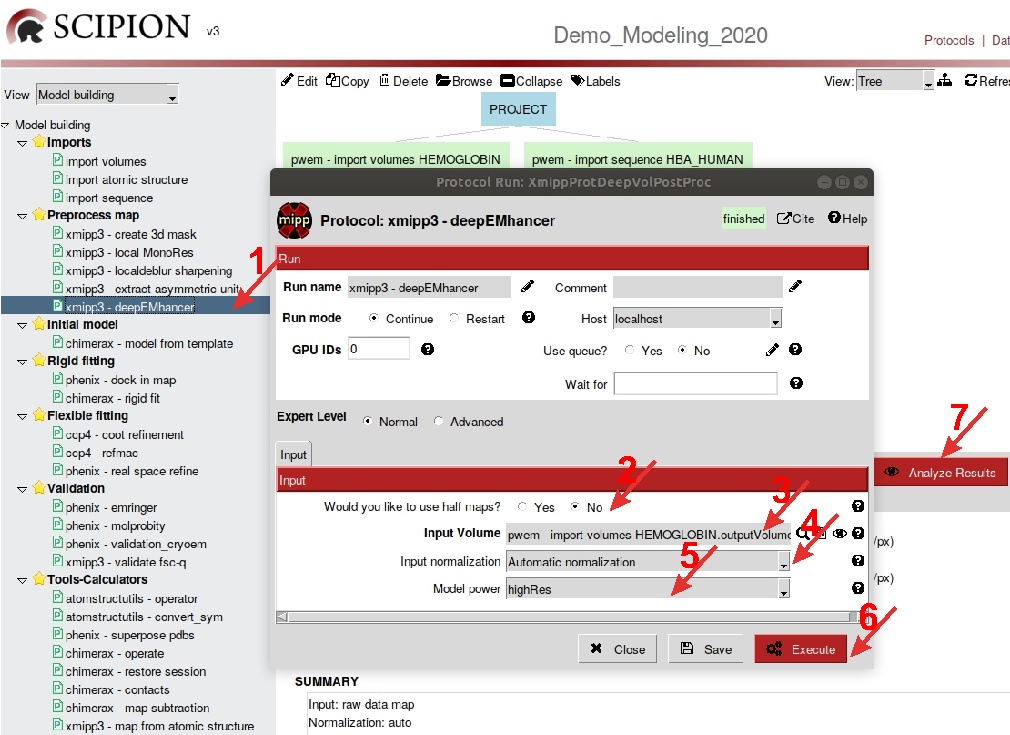
\includegraphics[width=0.95\textwidth]
  {Images/Fig63}
  \caption{Filling in the protocol to generate a sharpened map with $DeepEMhancer$.}
  \label{fig:deepEMHancer_1}
  \end{figure}

After executing the protocol (\ffigure{fig:deepEMHancer_1} (6)), we can check the results (7). \chimera viewer will open and show the sharpened map compared with the initial one (\ffigure{fig:deepEMHancer_2}).

\begin{figure}[H]
  \centering 
  \captionsetup{width=.9\linewidth} 
  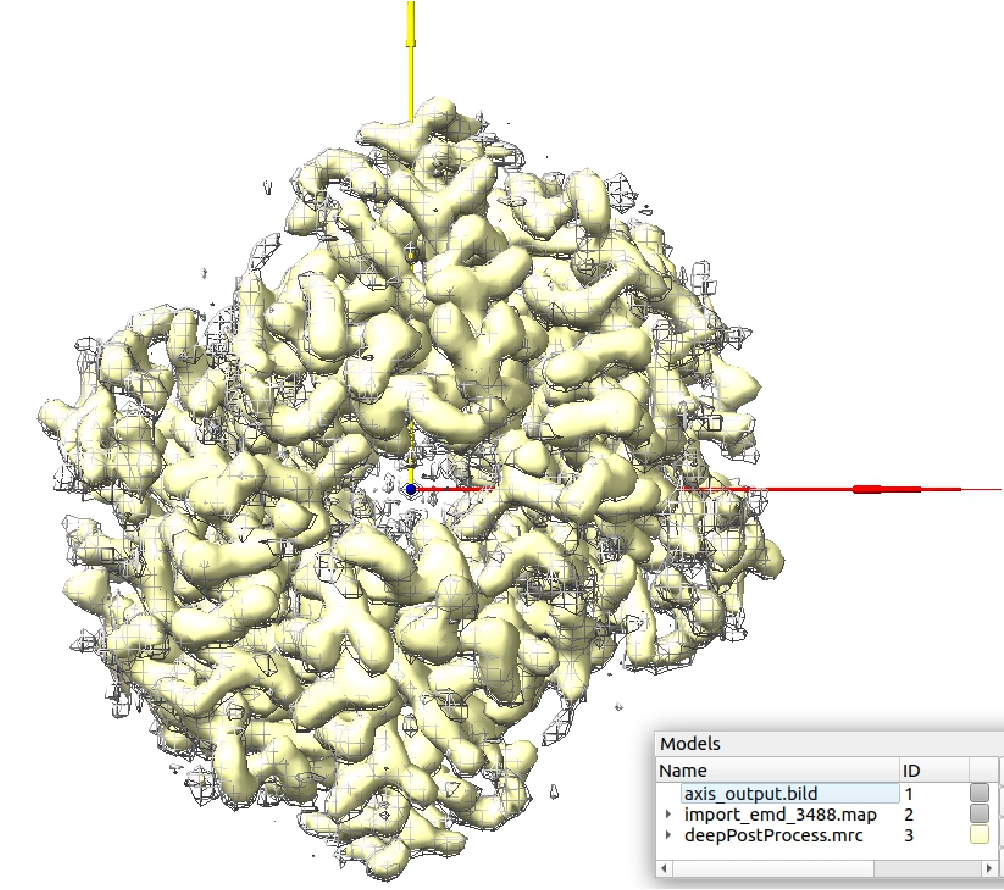
\includegraphics[width=0.65\textwidth]
  {Images/Fig65}
  \caption{$DeepEMhancer$ sharpened map (yellow surface) and input map (grey mesh) in \chimera.}
  \label{fig:deepEMHancer_2}
  \end{figure}
  
\subsection*{Comparison of maps}
Realize that at this point we have generated two optimized maps derived from the initial one. Additionally, some other maps could have been obtained using other map optimization methods. A comparison among them would be interesting to consider which one(s) of them should be used as input in next steps of modeling workflow. The ideal map for tracing the atomic structure should include as many details and connections as possible and, at the same time, preserve the density areas of the initial map. In other words, we can use the best sharpened map (with higher resolution) corroborating that it does not make up new densities, absent in the starting map. Nevertheless, choose ``the best'' sharpened map could be difficult sometimes, especially if the map is very big or there are some regions optimized in one of the sharpened maps and other areas optimized in the other one. In that case, you can use several maps at the same time, having all of them perfectly aligned according to the same origin of coordinates.

In the tiny example shown in this tutorial we are working with a high resolution map and there are almost no differences in resolution between the starting map and the two derived sharpened maps, although this is not usually the case in real life. In this quite uncommon case the initial unsharpened map would be enough to trace the atomic structure. However, in order to detail the method, the starting map and their two sharpened ones will be used simultaneously.




\subsection*{Extraction of the map asymmetric unit}
Since smaller volumes usually include lower number of individual structural elements, making easier fitting models in maps and simplifying modeling process, the part of the map chosen to work with will always be the smaller asymmetrical subunit of the starting loaded map, also known as asymmetric unit (ASU). The size of the ASU thus depends on the symmetry order of the initial volume. The higher the symmetry order, the smaller the ASU. The atomic structure of the whole volume will be obtained straight forward by simply repetition of the ASU structure according to the symmetry order. Then, the first step to simplify the complexity of the initial volume is extracting the ASU. This task can be accomplished by using the \scipion protocol \scommand{xmipp3 - extract unit cell} that extracts the geometrical ASU of the map (Appendix \ref{app:extractUnitCell}).\\

\ffigure{fig:extract_unit_cell} shows how to fill in this protocol form (1). Consider that in this particular case the protocol will be run three times, one with each map (the initial one and the two sharpened derived ones). Include each map in a protocol form parallel to that shown in \ffigure{fig:extract_unit_cell} (2). Since \ttt{metHgb} macromolecule shows symmetry C2, we have selected cyclic symmetry (Cn) as type of symmetry (3), and 2 as symmetry order (4). The angle offset selected (5) turns -45º around the Z axis the mask used to create the ASU. 
%Remark the relevance of including the offset in order to extract a unit cell able to reconstruct by symmetry the whole volume regarding the symmetry axes. 
The two wizards on the right (6, 7) help you to select the radii to delimit a fraction of the map comprised between the coordinate origin (inner radius 0.0) and the maximum radius (outer radius 50.0). The final extracted volume will be slightly higher than the ASU due to the expand factor 0.2 (8). % We use an expanded unit cell  to favor the modeling of each individual structure edges. 
The respective tutorial appendix \ref{app:extractUnitCell} includes a comprehensive explanation of the meaning of parameters. 

 \begin{figure}[H]
  \centering 
  \captionsetup{width=.9\linewidth} 
  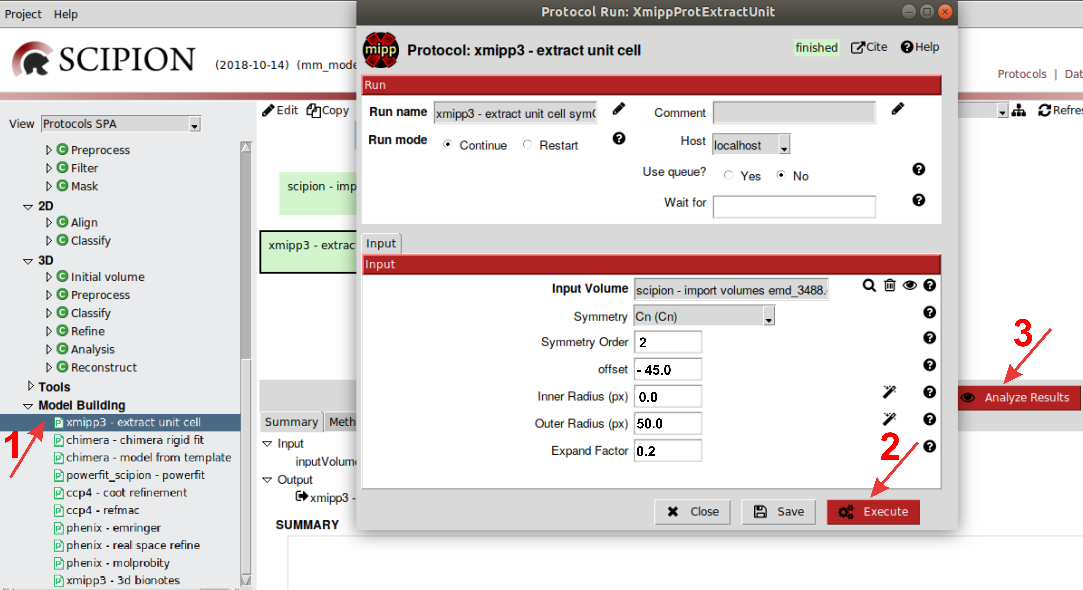
\includegraphics[width=1\textwidth]
  {Images/Fig7}
  \caption{Extracting the map asymmetric unit (ASU).}
  \label{fig:extract_unit_cell}
  \end{figure}
  
After executing the protocol (\ffigure{fig:extract_unit_cell}(9)), the resulting expanded ASU can be observed (10) with \chimera (\ffigure{fig:chimera_visualization_unit_cell}). Note the additional expanded volume of the  ASU on the left side of the figure. The ASU itself, on the right side, constitutes the half volume. Since the total volume contains the structure of four proteins, we can anticipate that this smaller asymmetrical subunit of the initial volume contains two proteins, one $\alpha$ and one $\beta$ \ttt{metHbg} subunits. Then, the respective structures of these two proteins could be fitted in the map ASU simultaneously or in successive modeling workflow steps. 
  
 \begin{figure}[H]
  \centering 
  \captionsetup{width=.9\linewidth} 
  \includegraphics[width=0.80\textwidth]
  {Images/Fig8}
  \caption{Expanded ASU (yellow-green-blue) and initial volume (gray) visualized with $ChimeraX$. The purple broken line on the right delimits the ASU (right) and its expanded volume (left).}
  \label{fig:chimera_visualization_unit_cell}
  \end{figure}

\section{Structure Prediction by Sequence Homology. Searching for Homologues}
\label{sec:structurePrediction}
As we have mentioned above, from the options indicated in the general workflow (\ffigure{fig:model_building_workflow}) to get initial models of structural elements, in this tutorial we are going to use tools to predict structure from sequence homology. 

Structure prediction by sequence homology only requires the sequence itself, from now ahead the \iii{target sequence}, and the access to databases to seek structures or \iii{templates} of homologous molecules. The sequences of homologous molecules show statistically significant similarity because they share common ancestry. Since the sequence encodes the structural information, from high similar sequences necessarily follows high similar structures. Structures from nearest homologous molecules will thus be preferred over remote relative ones. Remark that molecules containing several domains usually require independent searching for homologous templates of each domain. A small review about sequence similarity searching can be found in \citep{pearson2013}, and in \citep{kryshtafovych2018} the assessment of current \iii{template}-based modeling methods, many of them implemented as fully automated servers. Modeling tools appropriate to search for remote homologous \iii{templates}, folding recognition and \iii{template}-free methods (\iii{ab initio}), as well as $de\ novo$ modeling tools, which besides sequences use the volume itself, have still to be included in \scipion framework. 


\subsubsection*{How to identify \iii{templates} of the \iii{target sequence}}
 Similarity searching programs like \ttt{BLAST} (\ffigure{fig:blastp}) \citep{altschul1997}, available in \url{https://blast.ncbi.nlm.nih.gov/Blast.cgi}, use the \iii{target sequence} (1) to screen the structure-containing database \ttt{PDB} (2). Selecting or excluding a particular organism is an option (3). We usually start our searching selecting the organism in which we are interested or the closest evolutionarily related ones. If no similar sequences are found in these organisms, unrelated organisms may be selected or no one at all. Different searching algorithms are available (4) and one of them has to be selected. After executing \ttt{BLAST} (5) a list of score-ordered \iii{templates} is retrieved. 
 
  \begin{figure}[H]
  \centering 
  \captionsetup{width=.7\linewidth} 
  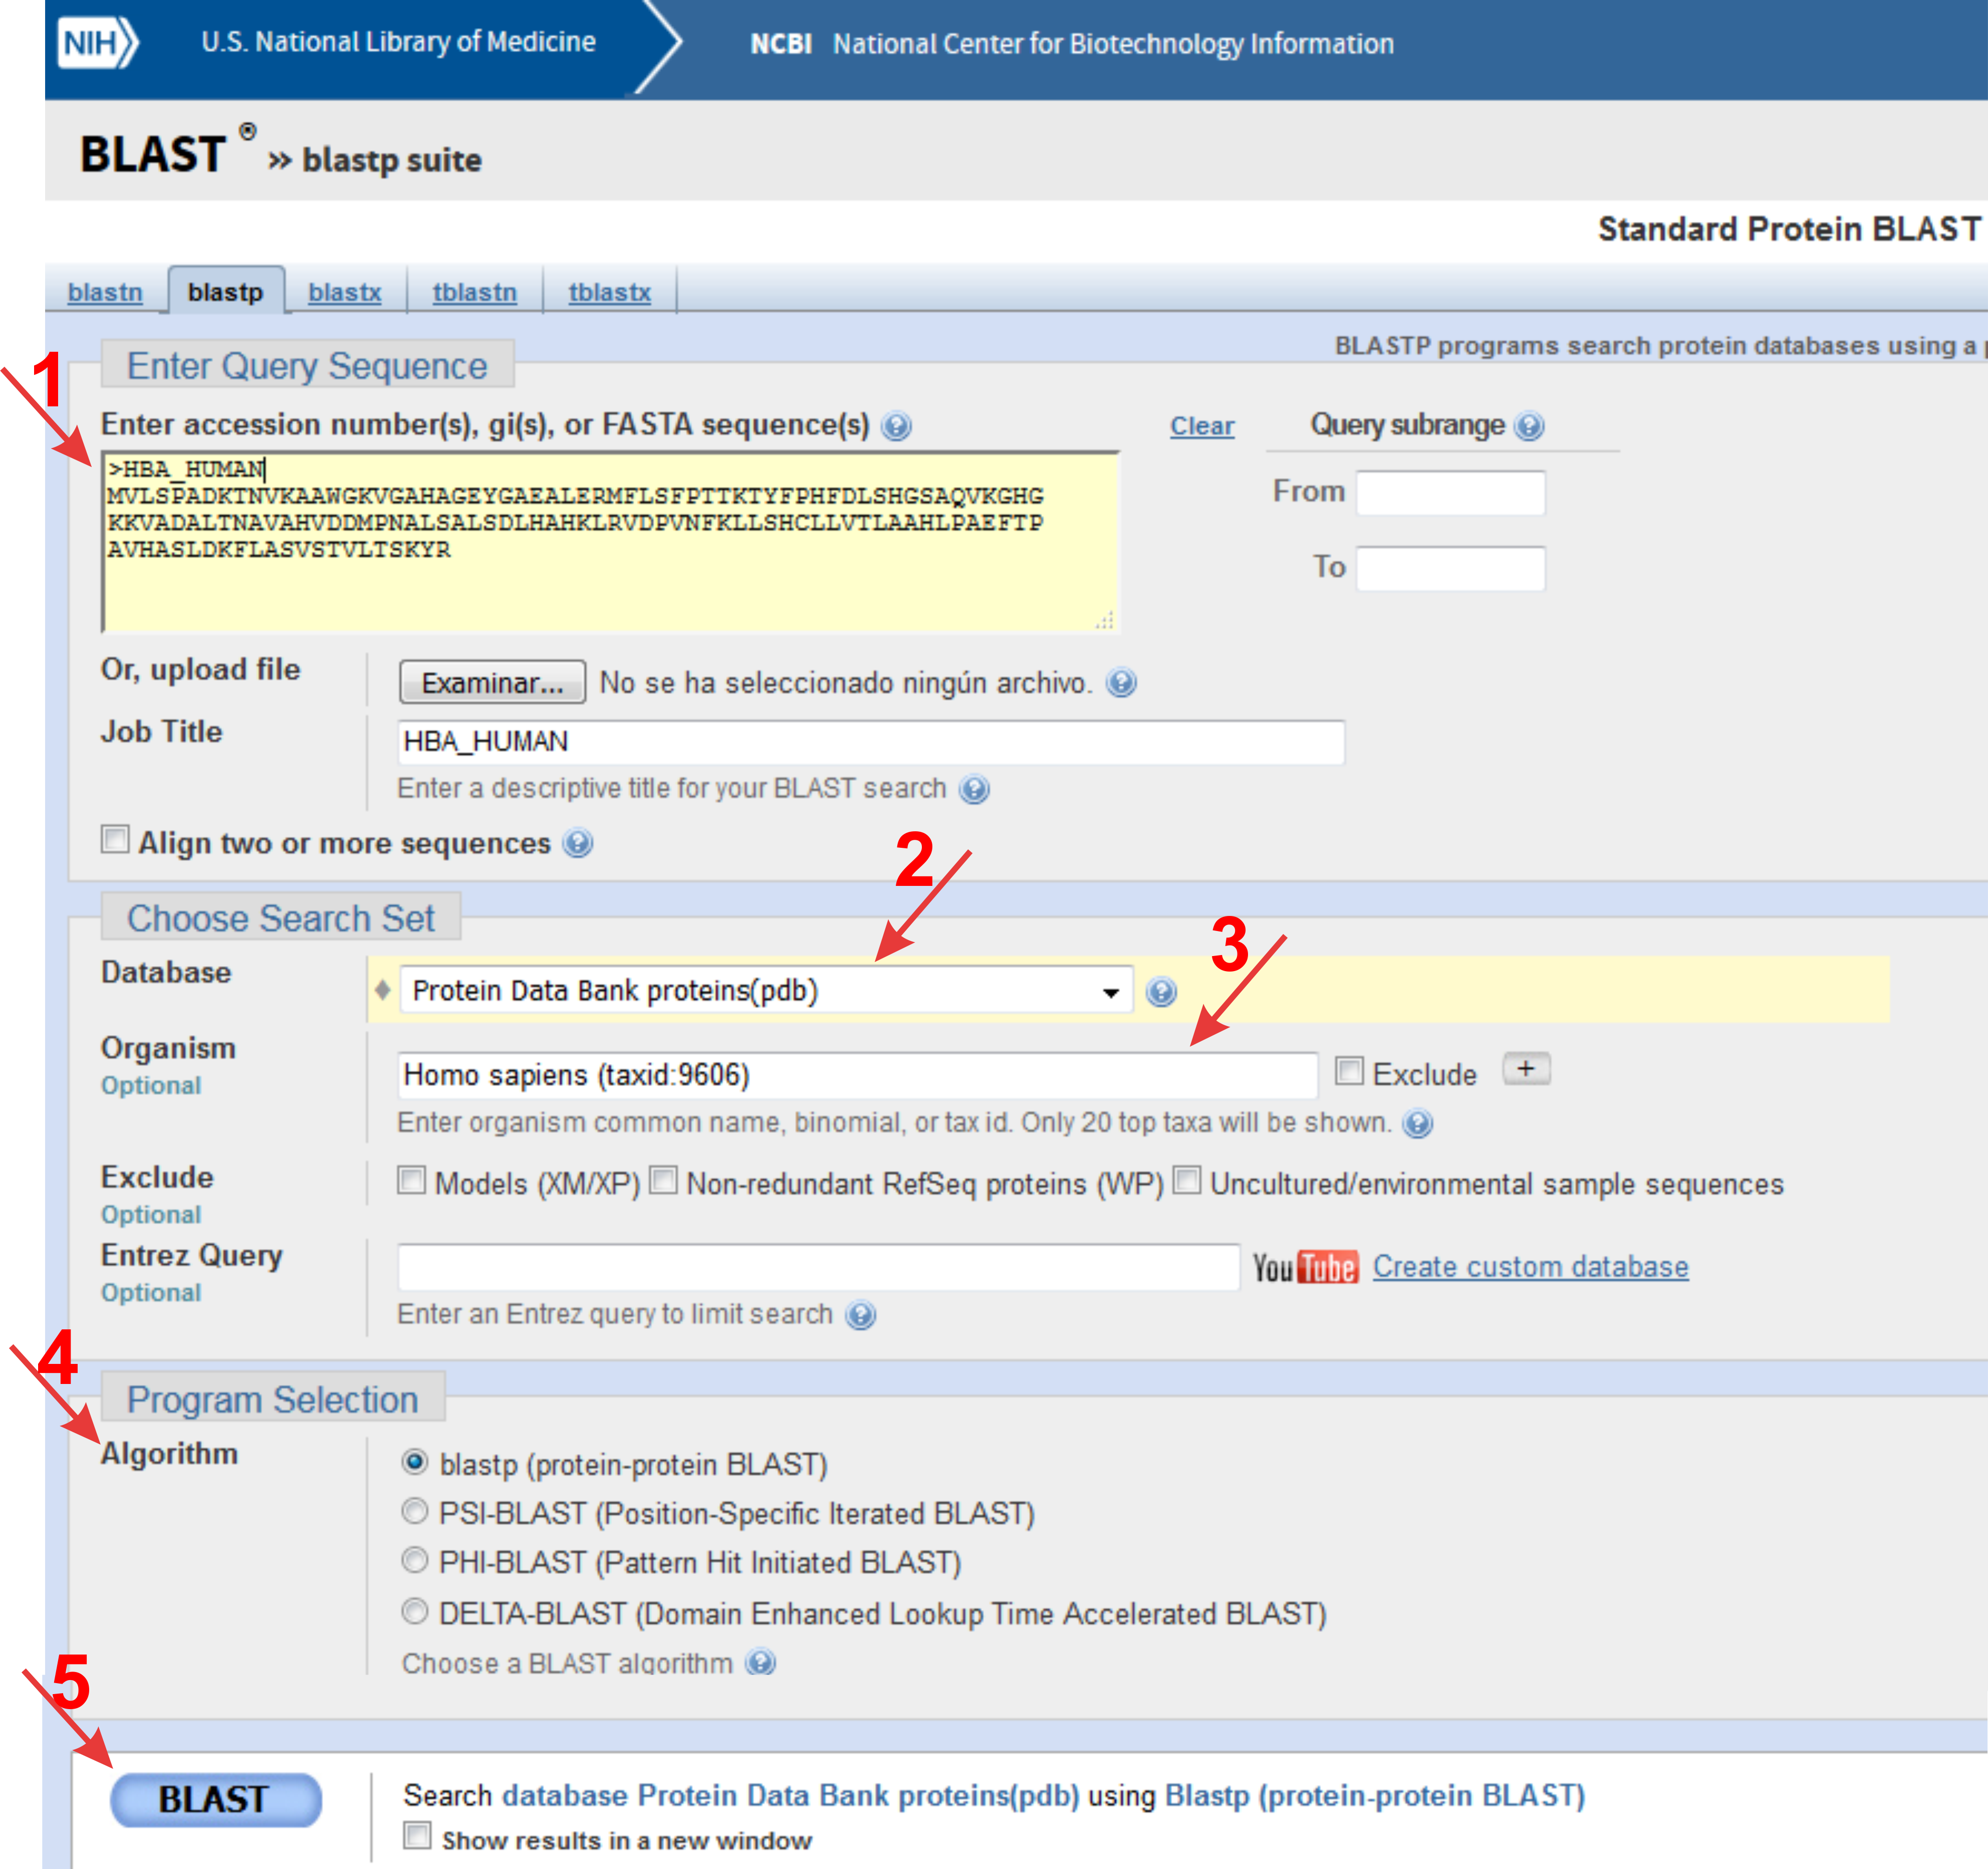
\includegraphics[width=0.80\textwidth]{Images/Fig9}
  \caption{Form of the similarity searching program \ttt{BLAST}.}
  \label{fig:blastp}
  \end{figure}
  
  Of course the closest relatives to human \ttt{Hgb} subunits, structurally characterized, will be their own structures contained in \ttt{PDB-5NI1}. However, in this tutorial we are going to assume that in our example the closest relatives to the human \ttt{Hgb} $\alpha$ and $\beta$ subunits are the respective \ttt{Hgb} subunits (identity 49.3\% and 45.21\%) of the antarctic fish \iii{Pagothenia bernacchii} \citep{camardella1992}. The atomic structure associated to this \iii{template} has \ttt{PDB} accession code \ttt{1PBX}. Information about the structure can be checked in \url{https://www.rcsb.org/structure/1PBX}. In general, it is a good idea to read the information related with the \iii{template}, do it so and answer the following questions: (Answers in appendix \ref{app:solutions}; \textbf{Question \ref{sec:structurePrediction}\_1})
  
  \begin{minipage}{\linewidth}
    \begin{framed}
      \begin{itemize}
        \item How has this structure been obtained (X-ray diffraction, EM, NMR)?
        \item What resolution does it have?
        \item How many chains does it include?
      \end{itemize}
    \end{framed}
  \end{minipage}

\section{Moving from sequence to atomic structure scenario}

\subsubsection*{Downloading the atomic structure}
  
  Once identified the \iii{template} that we are going to use as structural skeleton of our sequence, we import it into \scipion with the protocol \scommand{import atomic structure} (Appendix \ref{app:importAtomicStructure},  \ffigure{fig:import_atomic_structure} (1)). Select the option for importing the atomic structure from ID (2), write the \ttt{PDB} accession code (3) and execute the protocol (4). You can visualize the imported structure (5) in $Chimera$ (\ffigure{fig:chimera_visualization_structure}). By selecting chain \ttt{A} in the $Chimera$ upper menu (1) you can distinguish the \ttt{Hgb} $\alpha$ subunit (2).
  
  \begin{figure}[H]
  \centering 
  \captionsetup{width=.7\linewidth} 
  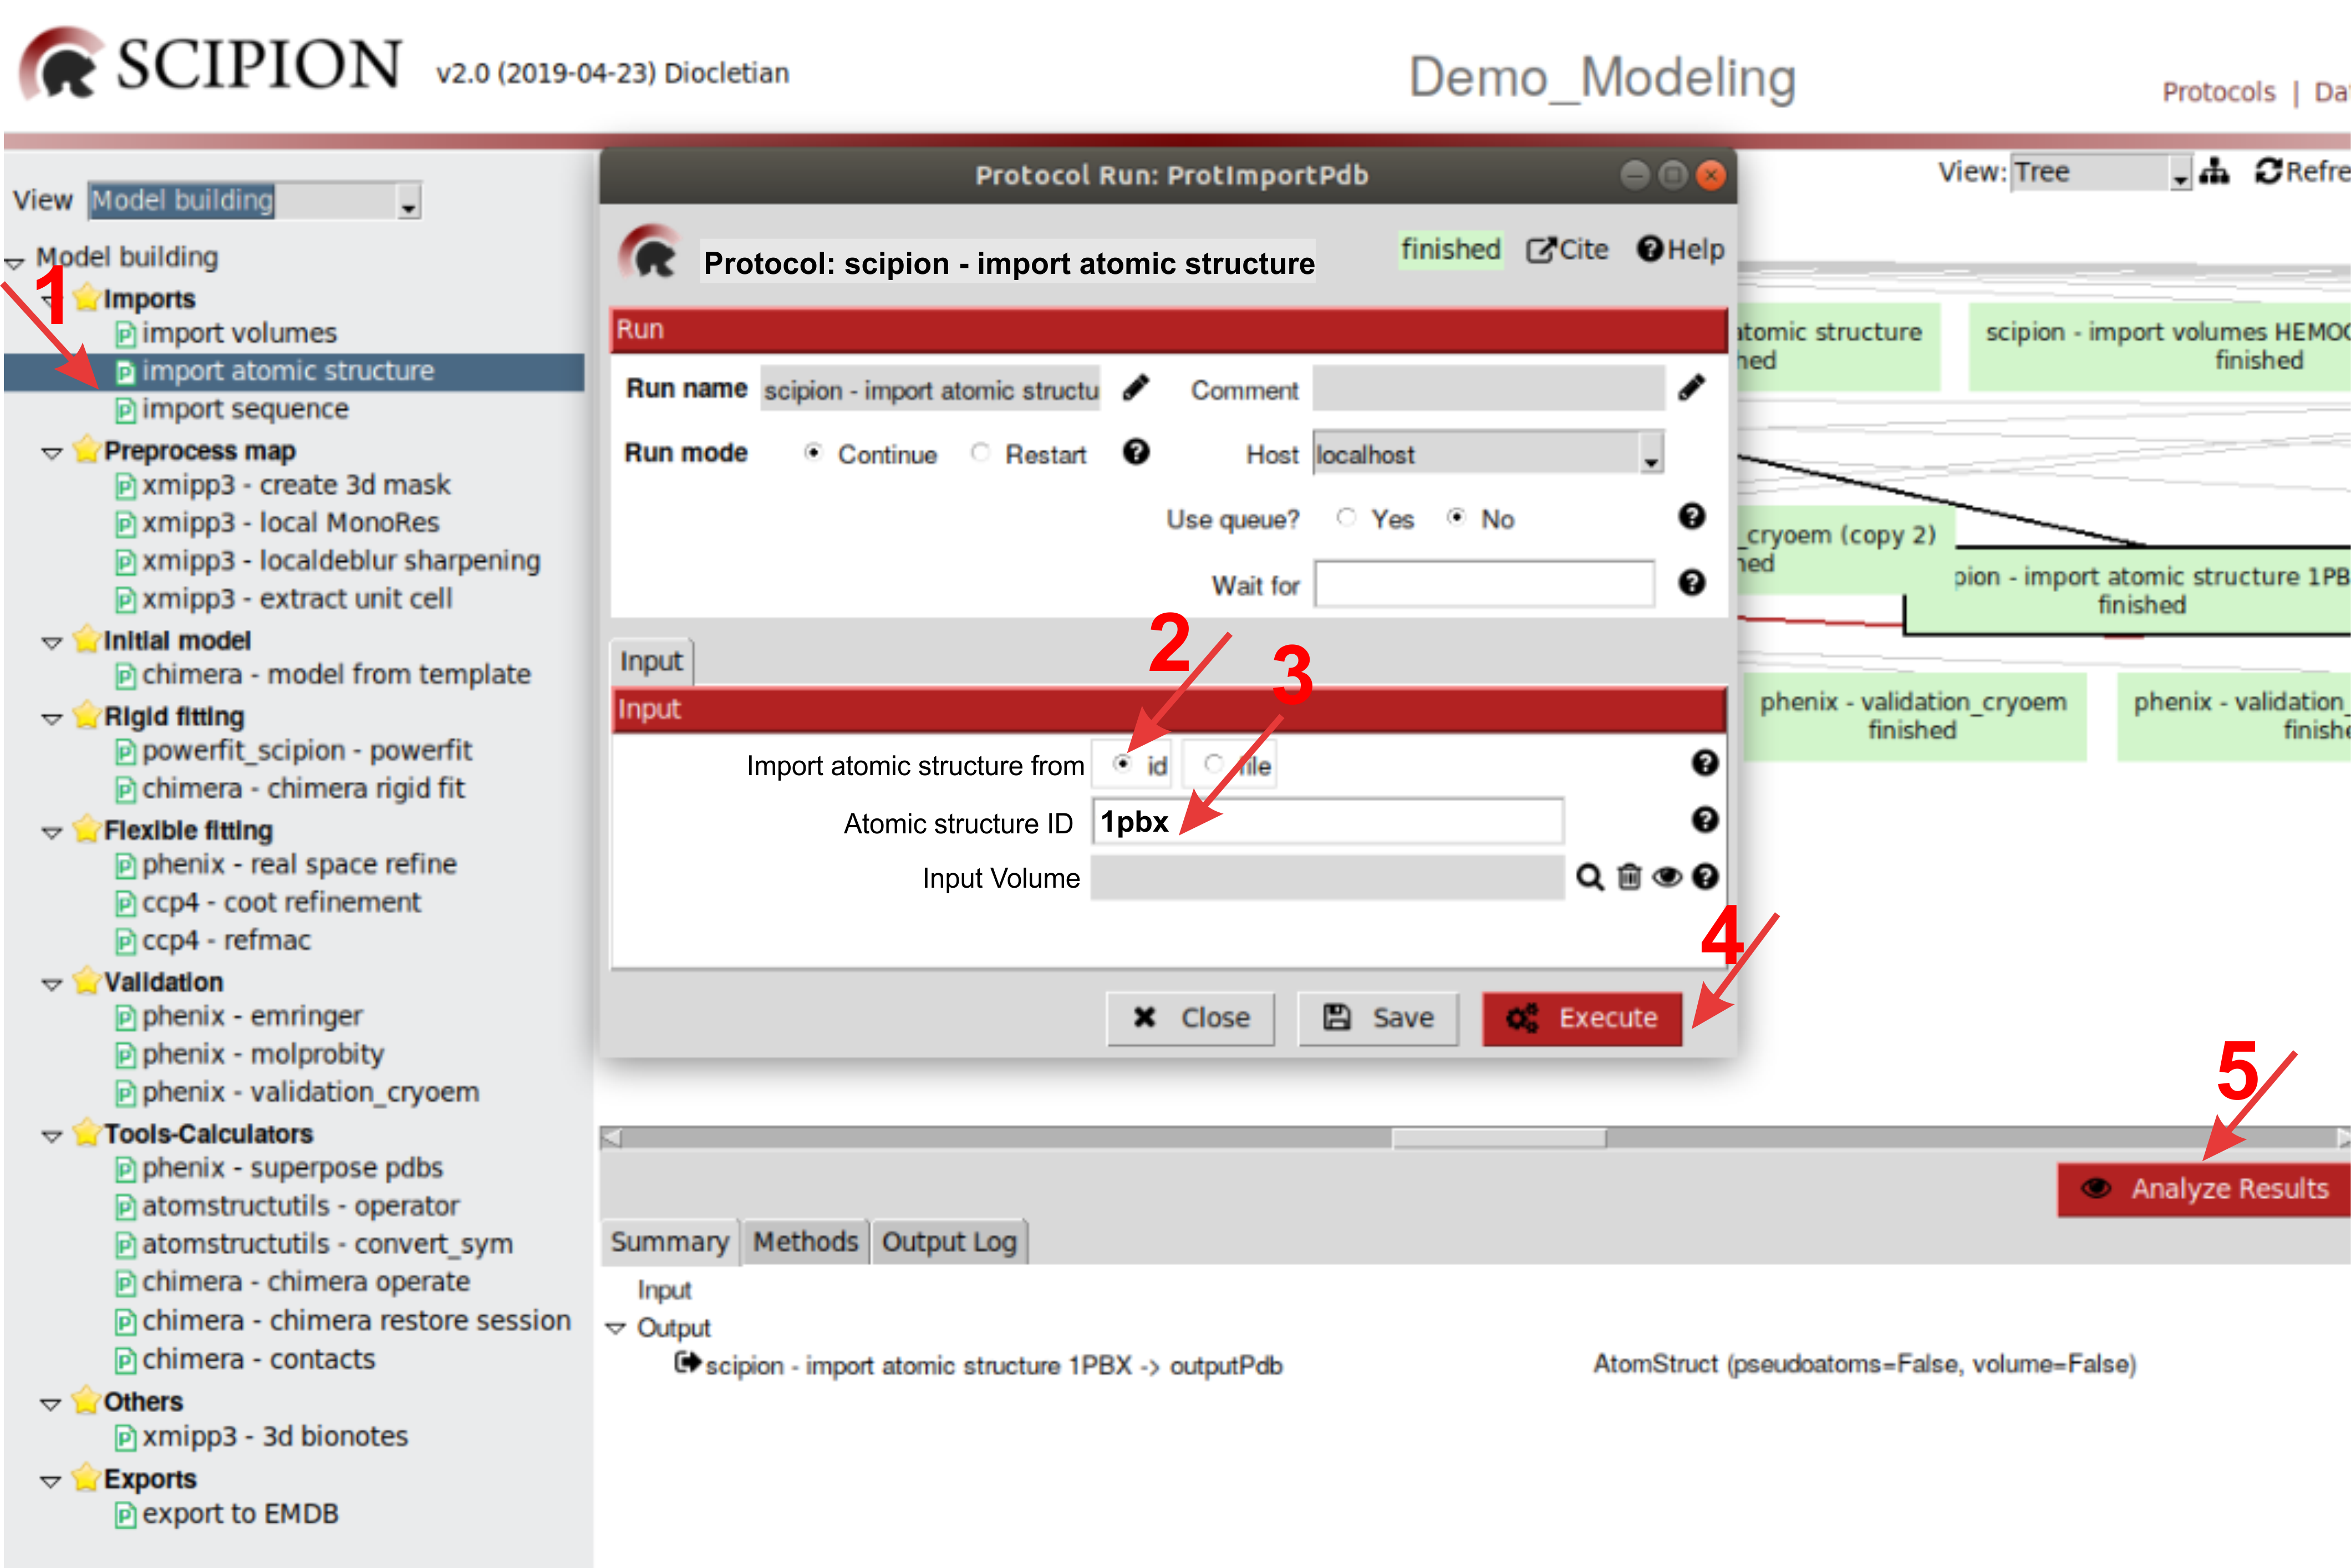
\includegraphics[width=0.90\textwidth]{Images/Fig10}
  \caption{Importing the atomic structure \ttt{1PBX}.}
  \label{fig:import_atomic_structure}
  \end{figure}
  
  \begin{figure}[H]
  \centering 
  \captionsetup{width=.7\linewidth} 
  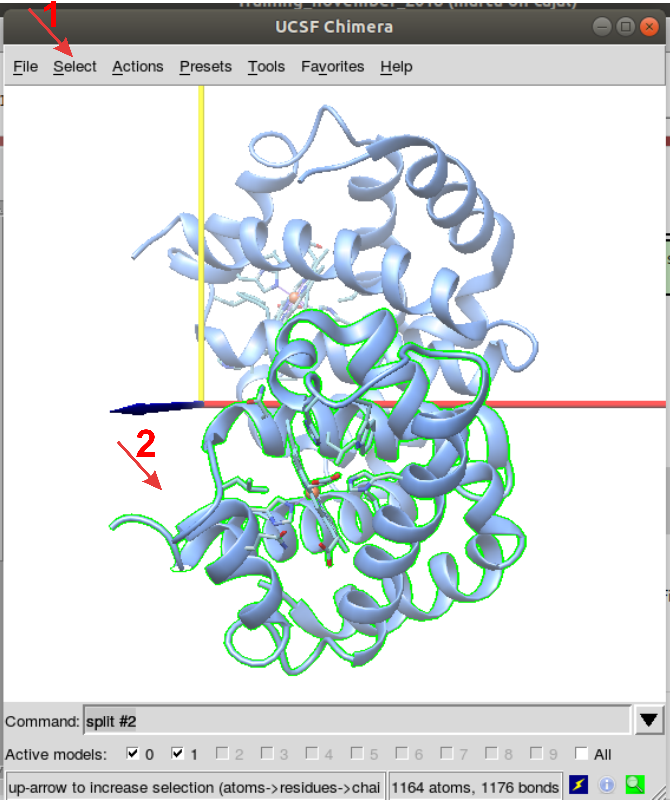
\includegraphics[width=0.50\textwidth]{Images/Fig11}
  \caption{Atomic structure \ttt{1PBX} visualized with Chimera. \ttt{Hgb} $\alpha$ subunit (chain \ttt{A}) is shown green-highlighted.}
  \label{fig:chimera_visualization_structure}
  \end{figure}
  
\subsubsection*{Structural models of human metHgb subunits from templates}

 $Modeller$ \citep{sali1993} is one of the computational web services used by $Chimera$, which provides the interface to run the program. Working with $Modeller$ requires a license key, which is provided free of charge for academic users. $Modeller$ allows two types of modeling computations to generate theoretical models, \iii{template}-based (sequence homology) and \iii{template}-free (\iii{de novo}, only for missing segments). In this tutorial we are going to consider the first one: structure prediction by sequence homology. Requirements for this type of modeling are the \iii{template} structure and a sequence alignment including sequences of \iii{target} and \iii{template}. 
 
 \begin{itemize}
 \item Preparing your sequence alignment:\\
In addition to the ways to obtain the \iii{target-template} sequence alignment using $Chimera$, this alignment can be also generated in the \scipion protocol \scommand{model from template} (Appendix \ref{app:modelFromTemplate}). This protocol allows selecting between pairwise and multiple sequence alignments. Besides producing more reliable alignments, especially for more distantly related sequences, multiple sequence alignments provide more structural information than pairwise alignments; they locate conserved regions in the molecule, thus improving predictions of structural arrangements due to mutant residues or residues that differ between \iii{template} and \iii{target} sequences \citep{pearson2013}. For this reason, in this tutorial we are going to perform a multiple sequence alignment. Additionally, you can also test the available tools to perform pairwise alignments.\\
 
Besides \iii{target} and \iii{template} sequence, some more sequences are needed to accomplish a multiple sequence alignment. The type and number of the sequences included depends on the sequence conservation, although they have to allow differentiating conserved regions. As an example, our multiple sequence alignment will include four more \ttt{Hgb} $\alpha$ subunit sequences from organisms located between human and fish in the evolutionary scale: \iii{Equus caballus} (Horse), \iii{Oryctolagus cuniculus} (Rabbit), \iii{Meleagris gallopavo} (Wild turkey), \iii{Aldabrachelys gigantea} (Aldabra giant tortoise). Download these sequences one by one from \ttt{UniProtKB} database filling in the \scommand{import sequence} protocol form with the appropriate accession codes (\ffigure{fig:multialignment_sequences}). A similar process has to be followed for \ttt{Hgb} $\beta$ subunit, importing \ttt{UniProtKB} sequences \ttt{P02062 (HBB\_HORSE), P02057(HBB\_RABIT), G1U9Q8 (G1U9Q8\_MELGA)} and \ttt{P83133 (HBB\_ALDGI)}.

  \begin{figure}[H]
  \centering 
  \captionsetup{width=.7\linewidth} 
  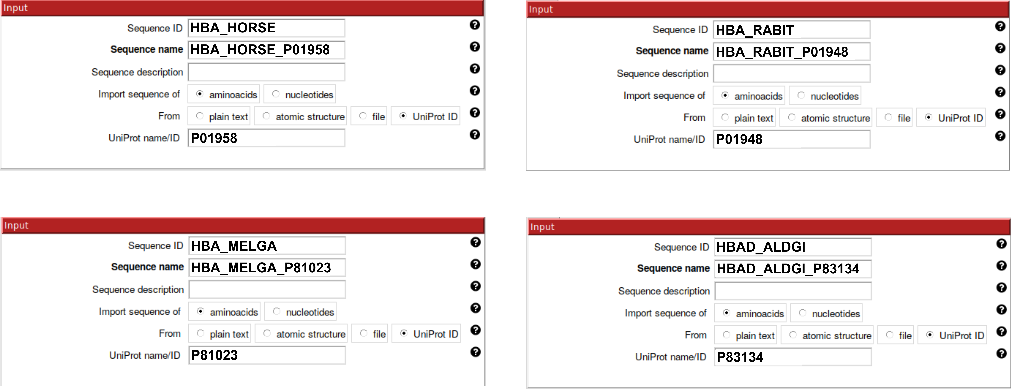
\includegraphics[width=0.95\textwidth]{Images/Fig12}
  \caption{Importing additional sequences to perform the multiple sequence alignment.}
  \label{fig:multialignment_sequences}
  \end{figure}

 \item Access to $Modeller$ in $Chimera$:\\
 The protocol \scommand{model from template} allows direct opening of the multiple sequence alignment in $Chimera$ and then, access to $Modeller$ via web service. Fill in the protocol form (\ffigure{fig:model_from_template_protocol} (1)), including the \iii{template} \ttt{1PBX} previously imported (2), the particular chain of interest (use the wizard to select it (3)) and the \iii{target} sequence of human \ttt{Hgb} $\alpha$ subunit (4). Since we plan to perform a multiple sequence alignment, we'd like to include additional sequences to align (5), that have to add next (6). Finally, select one of the multiple sequence alignment tools (7). 
 
 \begin{figure}[H]
  \centering 
  \captionsetup{width=.7\linewidth} 
  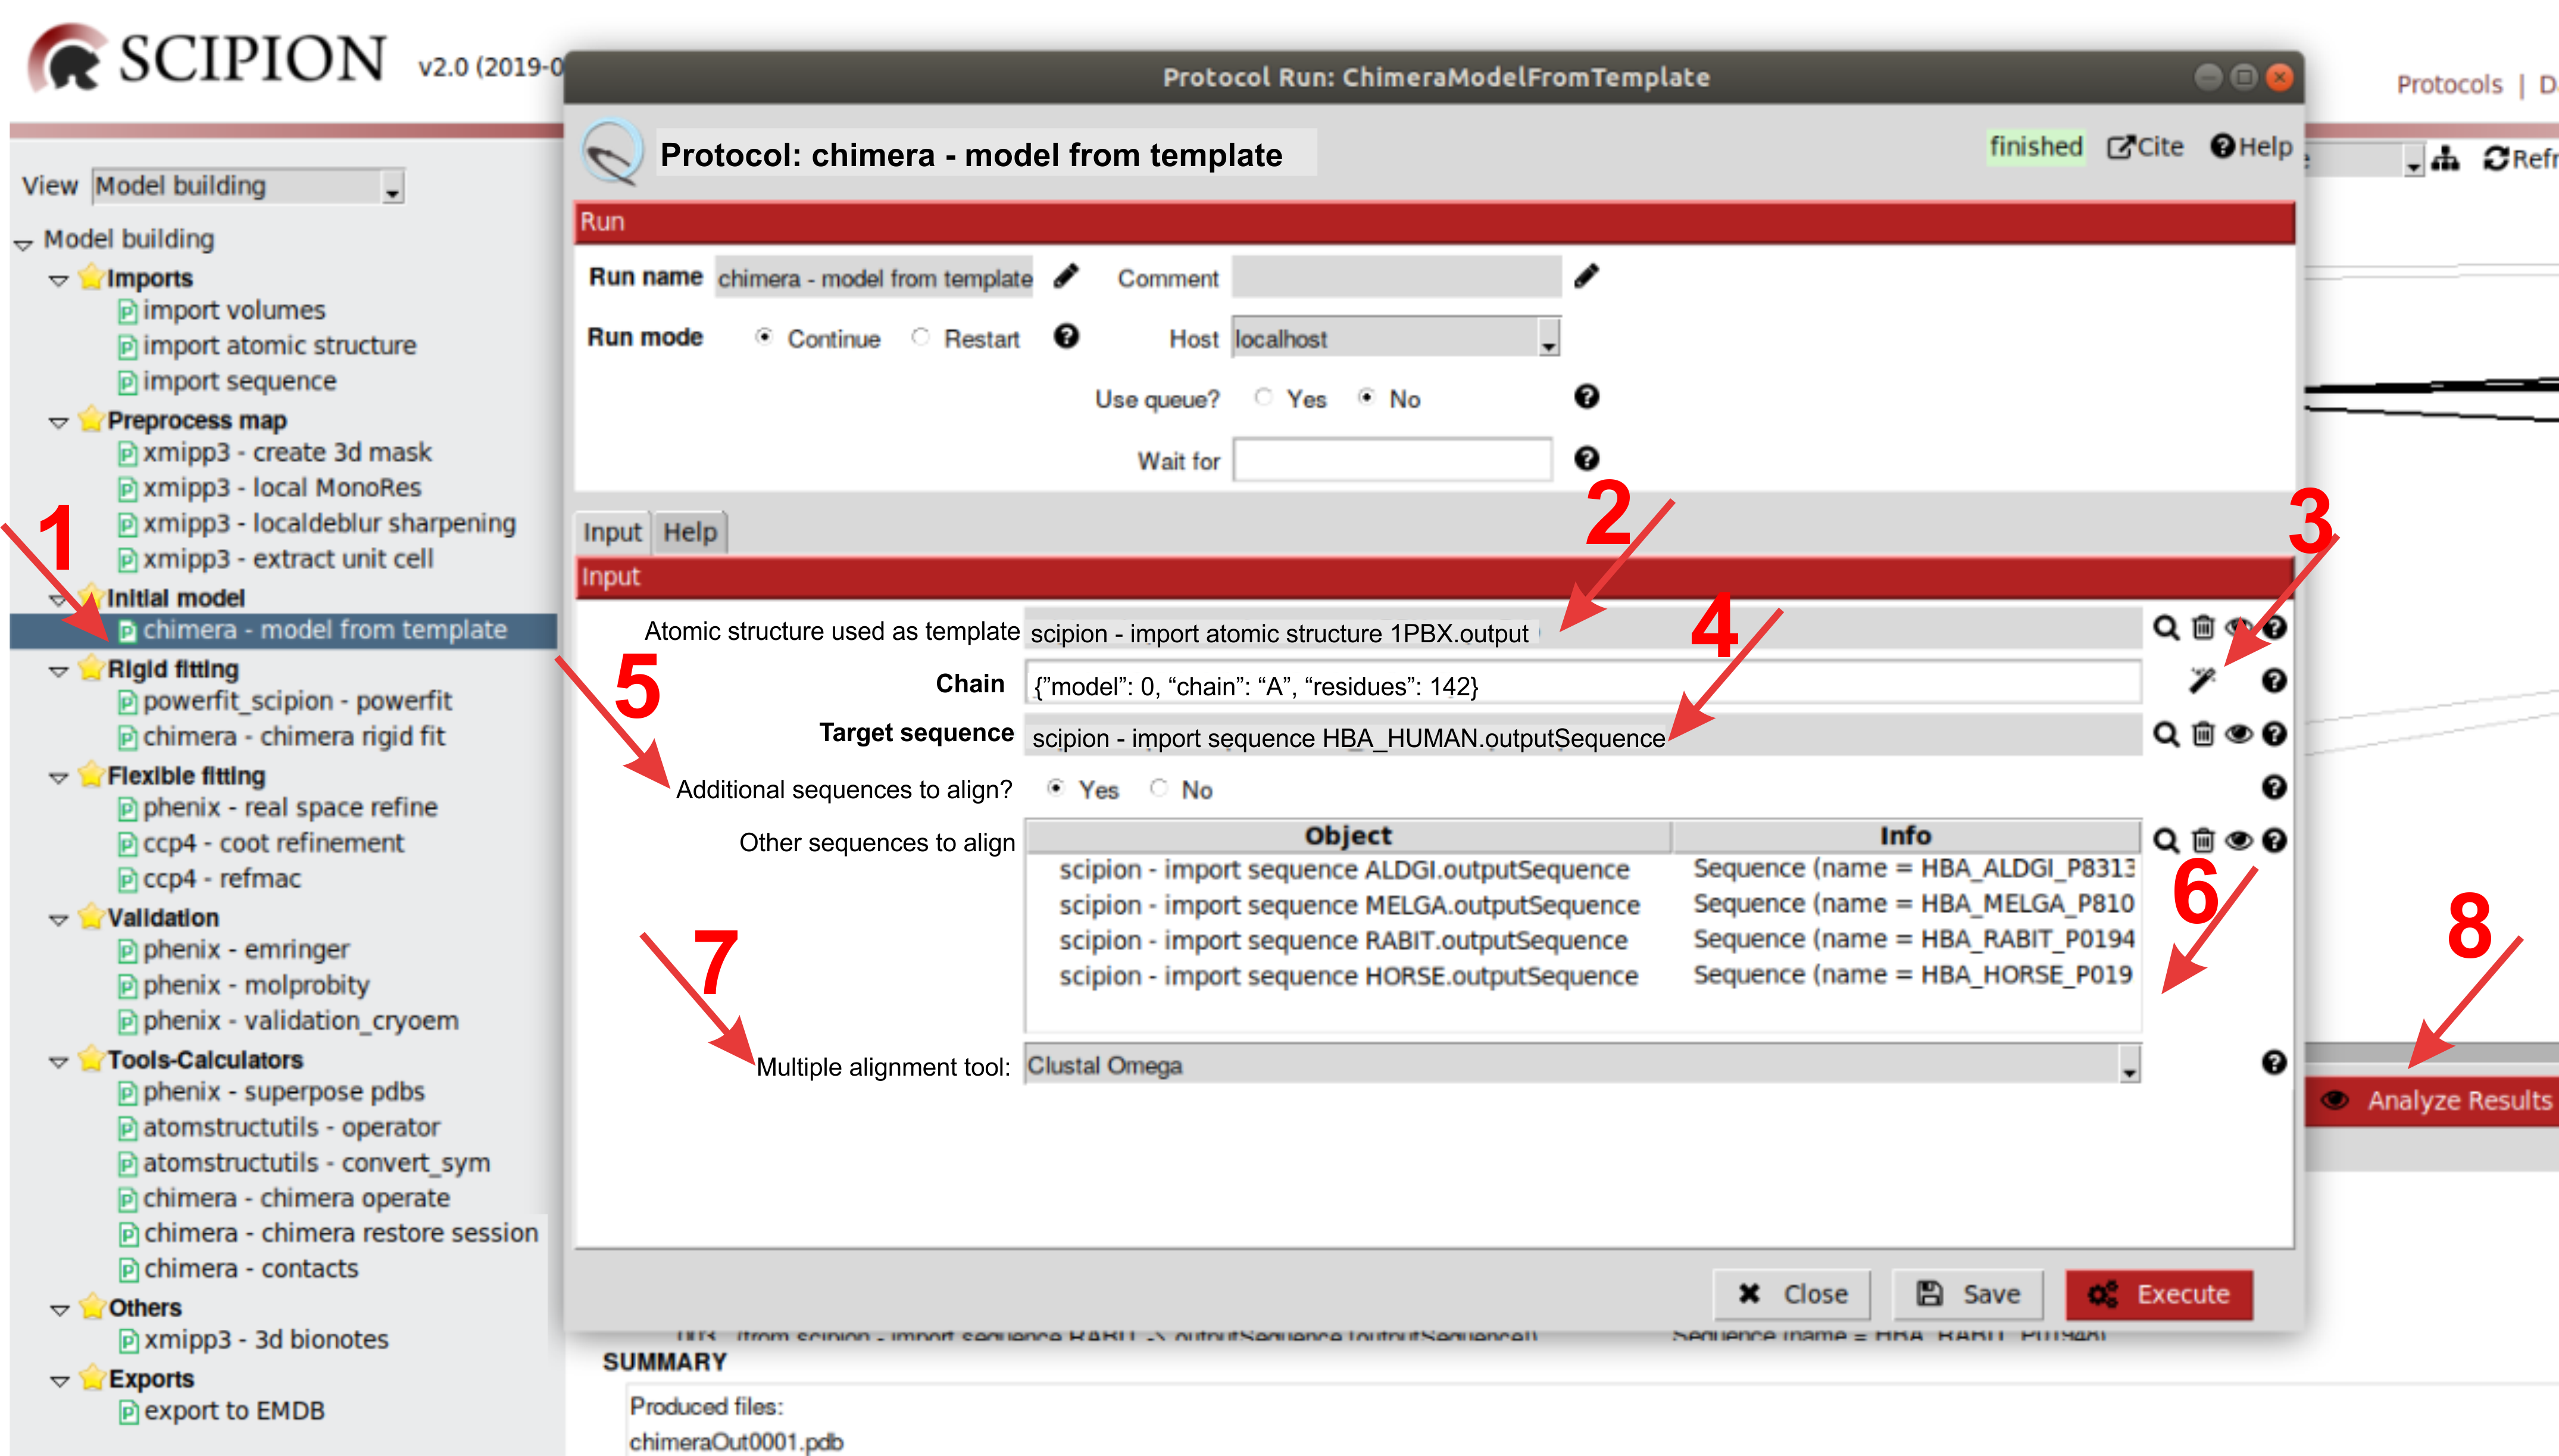
\includegraphics[width=0.90\textwidth]{Images/Fig13}
  \caption{Importing the multiple sequence alignment in $Chimera$.}
  \label{fig:model_from_template_protocol}
  \end{figure}
 
 A couple of windows will be open, the multiple sequence alignment in the upper part of \ffigure{fig:chimera_alignment}, and $Chimera$ graphics window. The \iii{template} selected chain is shown green-highlighted in both windows. As you may observe in the alignment, \ttt{Hgb} $\alpha$ subunit is a quite conserved macromolecule; there is only one gap in the alignment because \ttt{PRO} (Proline) 47 residue has disappeared during evolution. Human \ttt{Hgb} $\alpha$ subunit is closer to the protein in mammals (horse, rabbit) than to the protein in unrelated organisms, as we would have anticipated. Corroborate this point by checking the identity percentage \%ID  between human sequence and the other sequences in \ffigure{fig:modeller} (B). 
 
 \begin{figure}[H]
  \centering 
  \captionsetup{width=.7\linewidth} 
  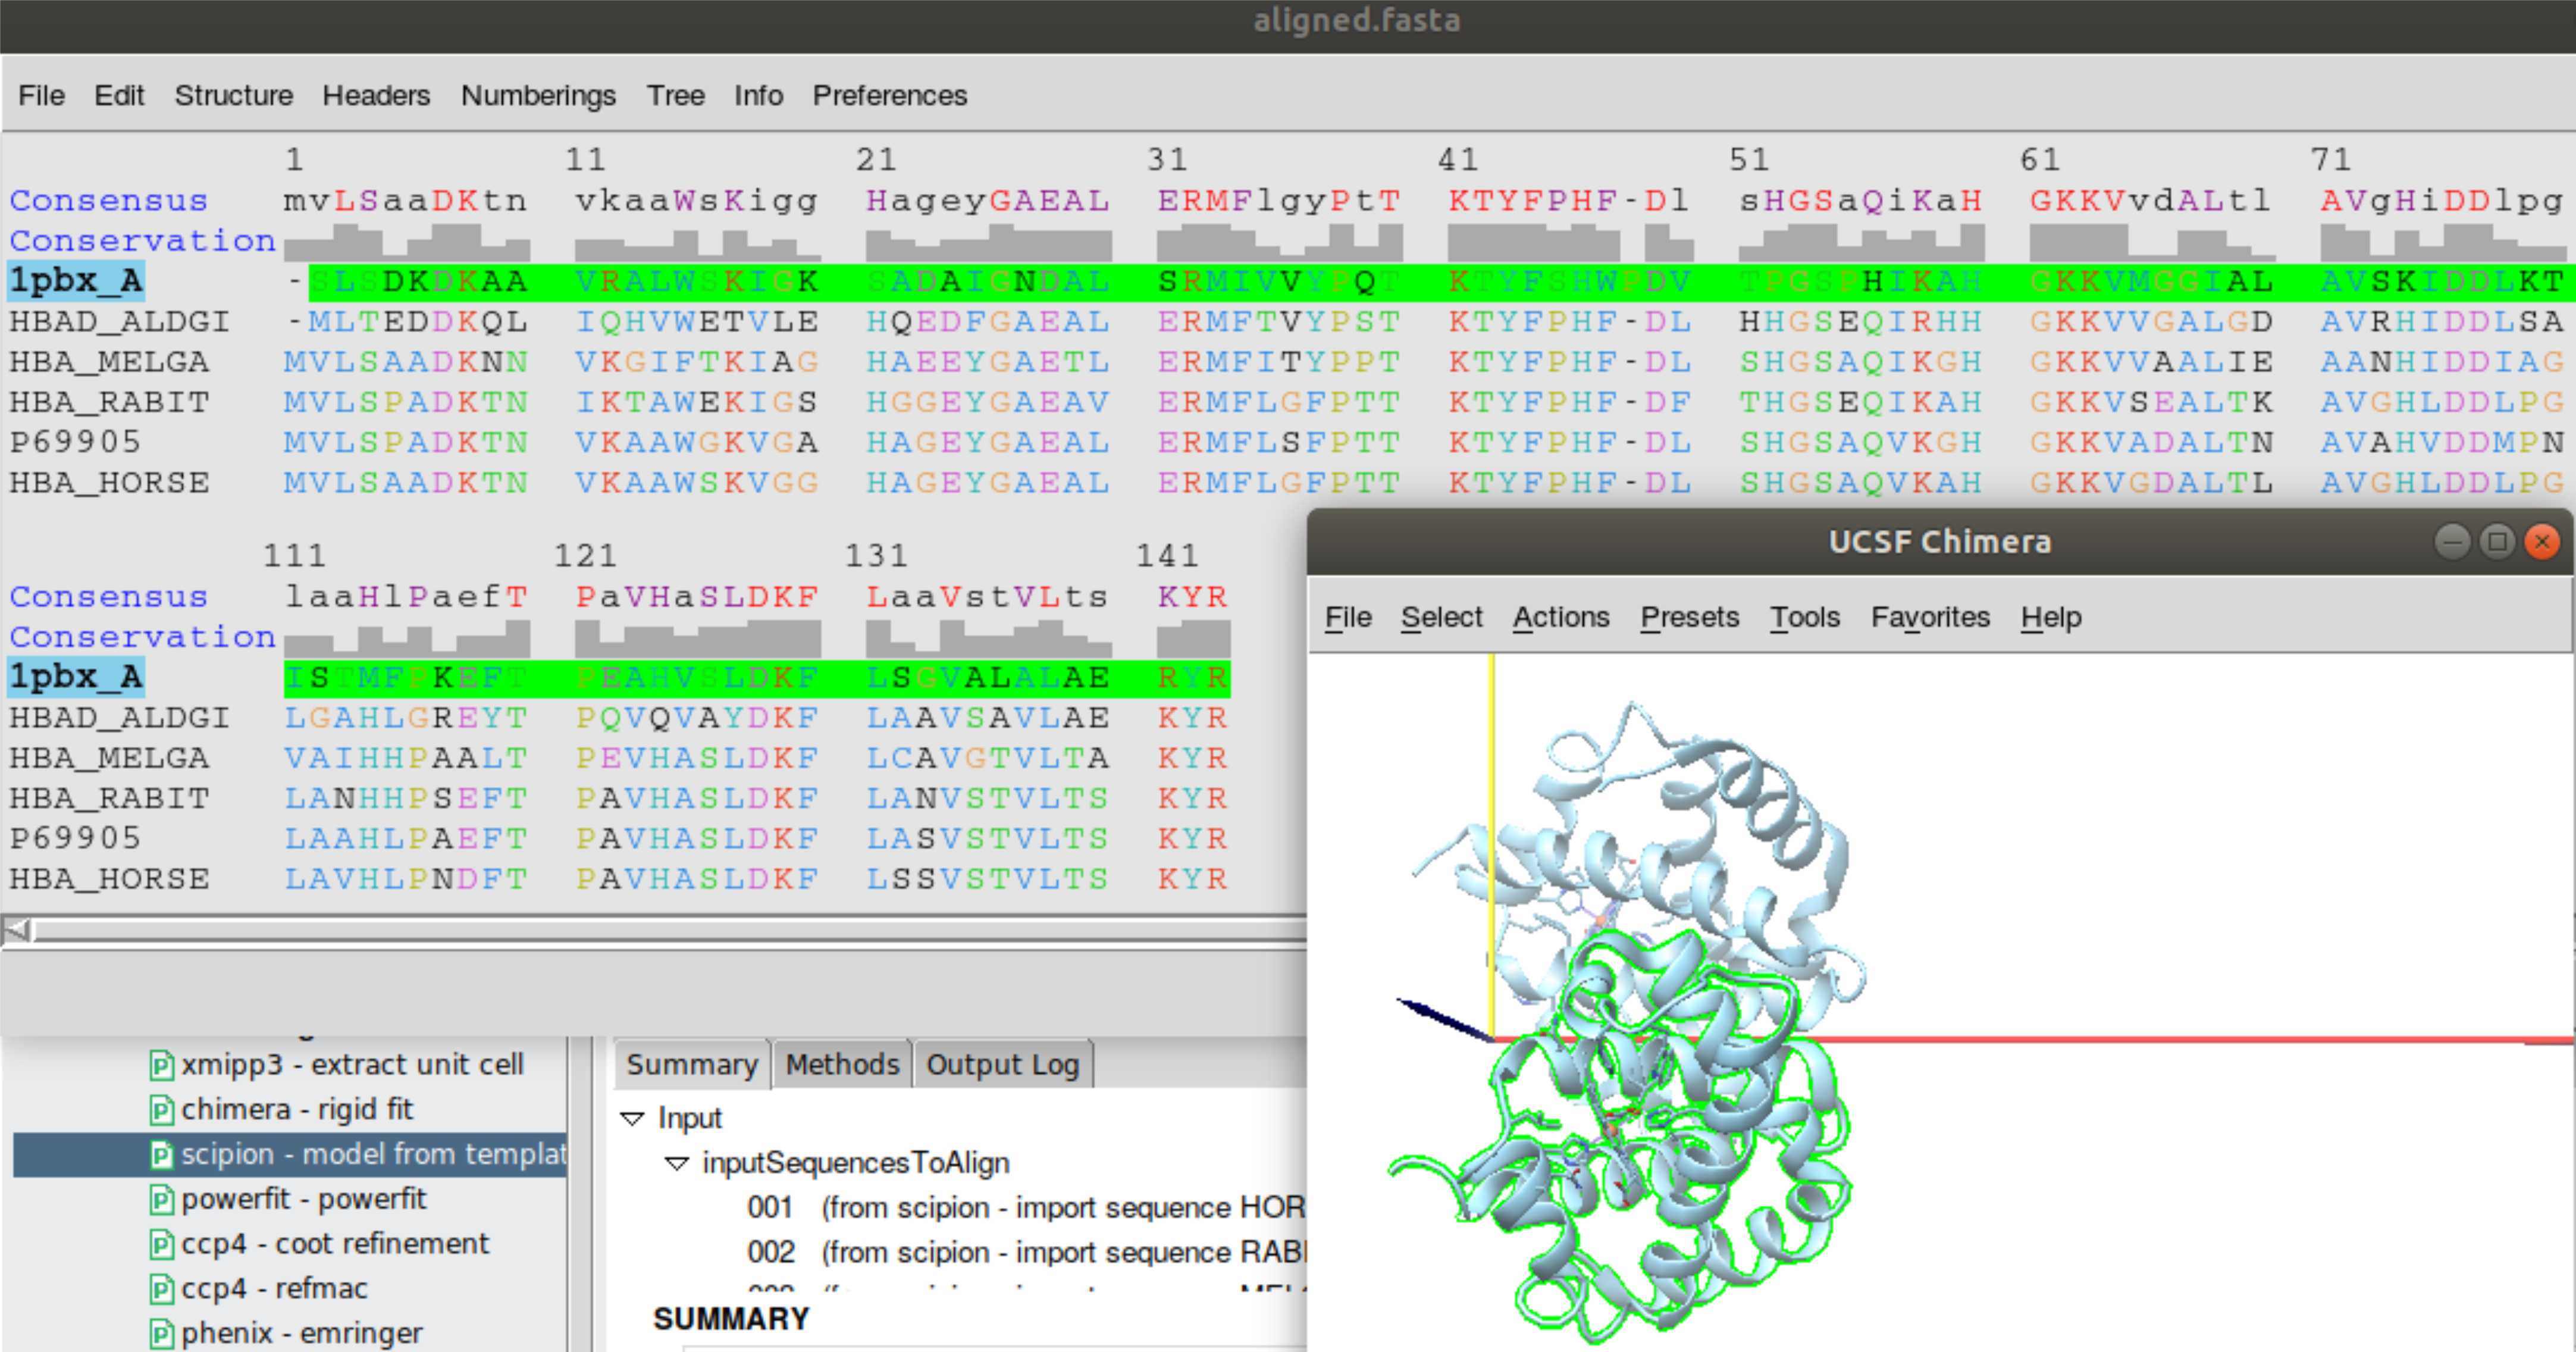
\includegraphics[width=0.80\textwidth]{Images/Fig14}
  \caption{Opening the multiple sequence alignment in $Chimera$.}
  \label{fig:chimera_alignment}
  \end{figure}
\end{itemize}

In case you'd like edit the name or the order of the sequences, add,  delete or realign sequences, ..., go to the upper menu of the multiple sequence alignment (\ttt{Edit -> }). In particular, we are going to change the name of the \iii{target} sequence from \ttt{P69905} to \ttt{HBA\_HUMAN} in \ttt{Edit -> Edit Sequence Name...} (\ffigure{fig:modeller} (A)). To get possible atomic models of the \iii{target} sequence in $Modeller$ web service, we have to select \ttt{Structure -> Modeller (homology ...)} in the same upper menu. A new window for Comparative Modeling with Modeller will be open (\ffigure{fig:modeller} (B)), that we have to fill in selecting \iii{target} sequence (1) and \iii{template} (2). Modeller license key has to be included here (3). The number of output models can be specified in Advanced Options (5 by default). Finally, press Apply to start the computation without hide the panel (4) or OK to start the computation hiding it. In $Chimera$ main graphics window, lower left corner, you may see the status of your job. After a while, five possible atomic structures, from now ahead \iii{models}, are retrieved for the \iii{target} sequence (\ffigure{fig:modeller} (C)) together with their assessment scores. Column \ttt{GA341} of Modeller Results indicates the score derived from statistical potentials (values in \ttt{[0,1]}; \ttt{> 0.7} for reliable \iii{models}). Column \ttt{zDOPE} (normalized Discrete Optimized Protein Energy) score depends on the atomic distance (negative values for the better \iii{models}). Let's select \iii{model} \ttt{\#2.1}. You can check every model numbers in $Chimera$'s main menu (\ttt{Favorites -> Model Panel}).
 
  \begin{figure}[H]
  \centering 
  \captionsetup{width=.7\linewidth} 
  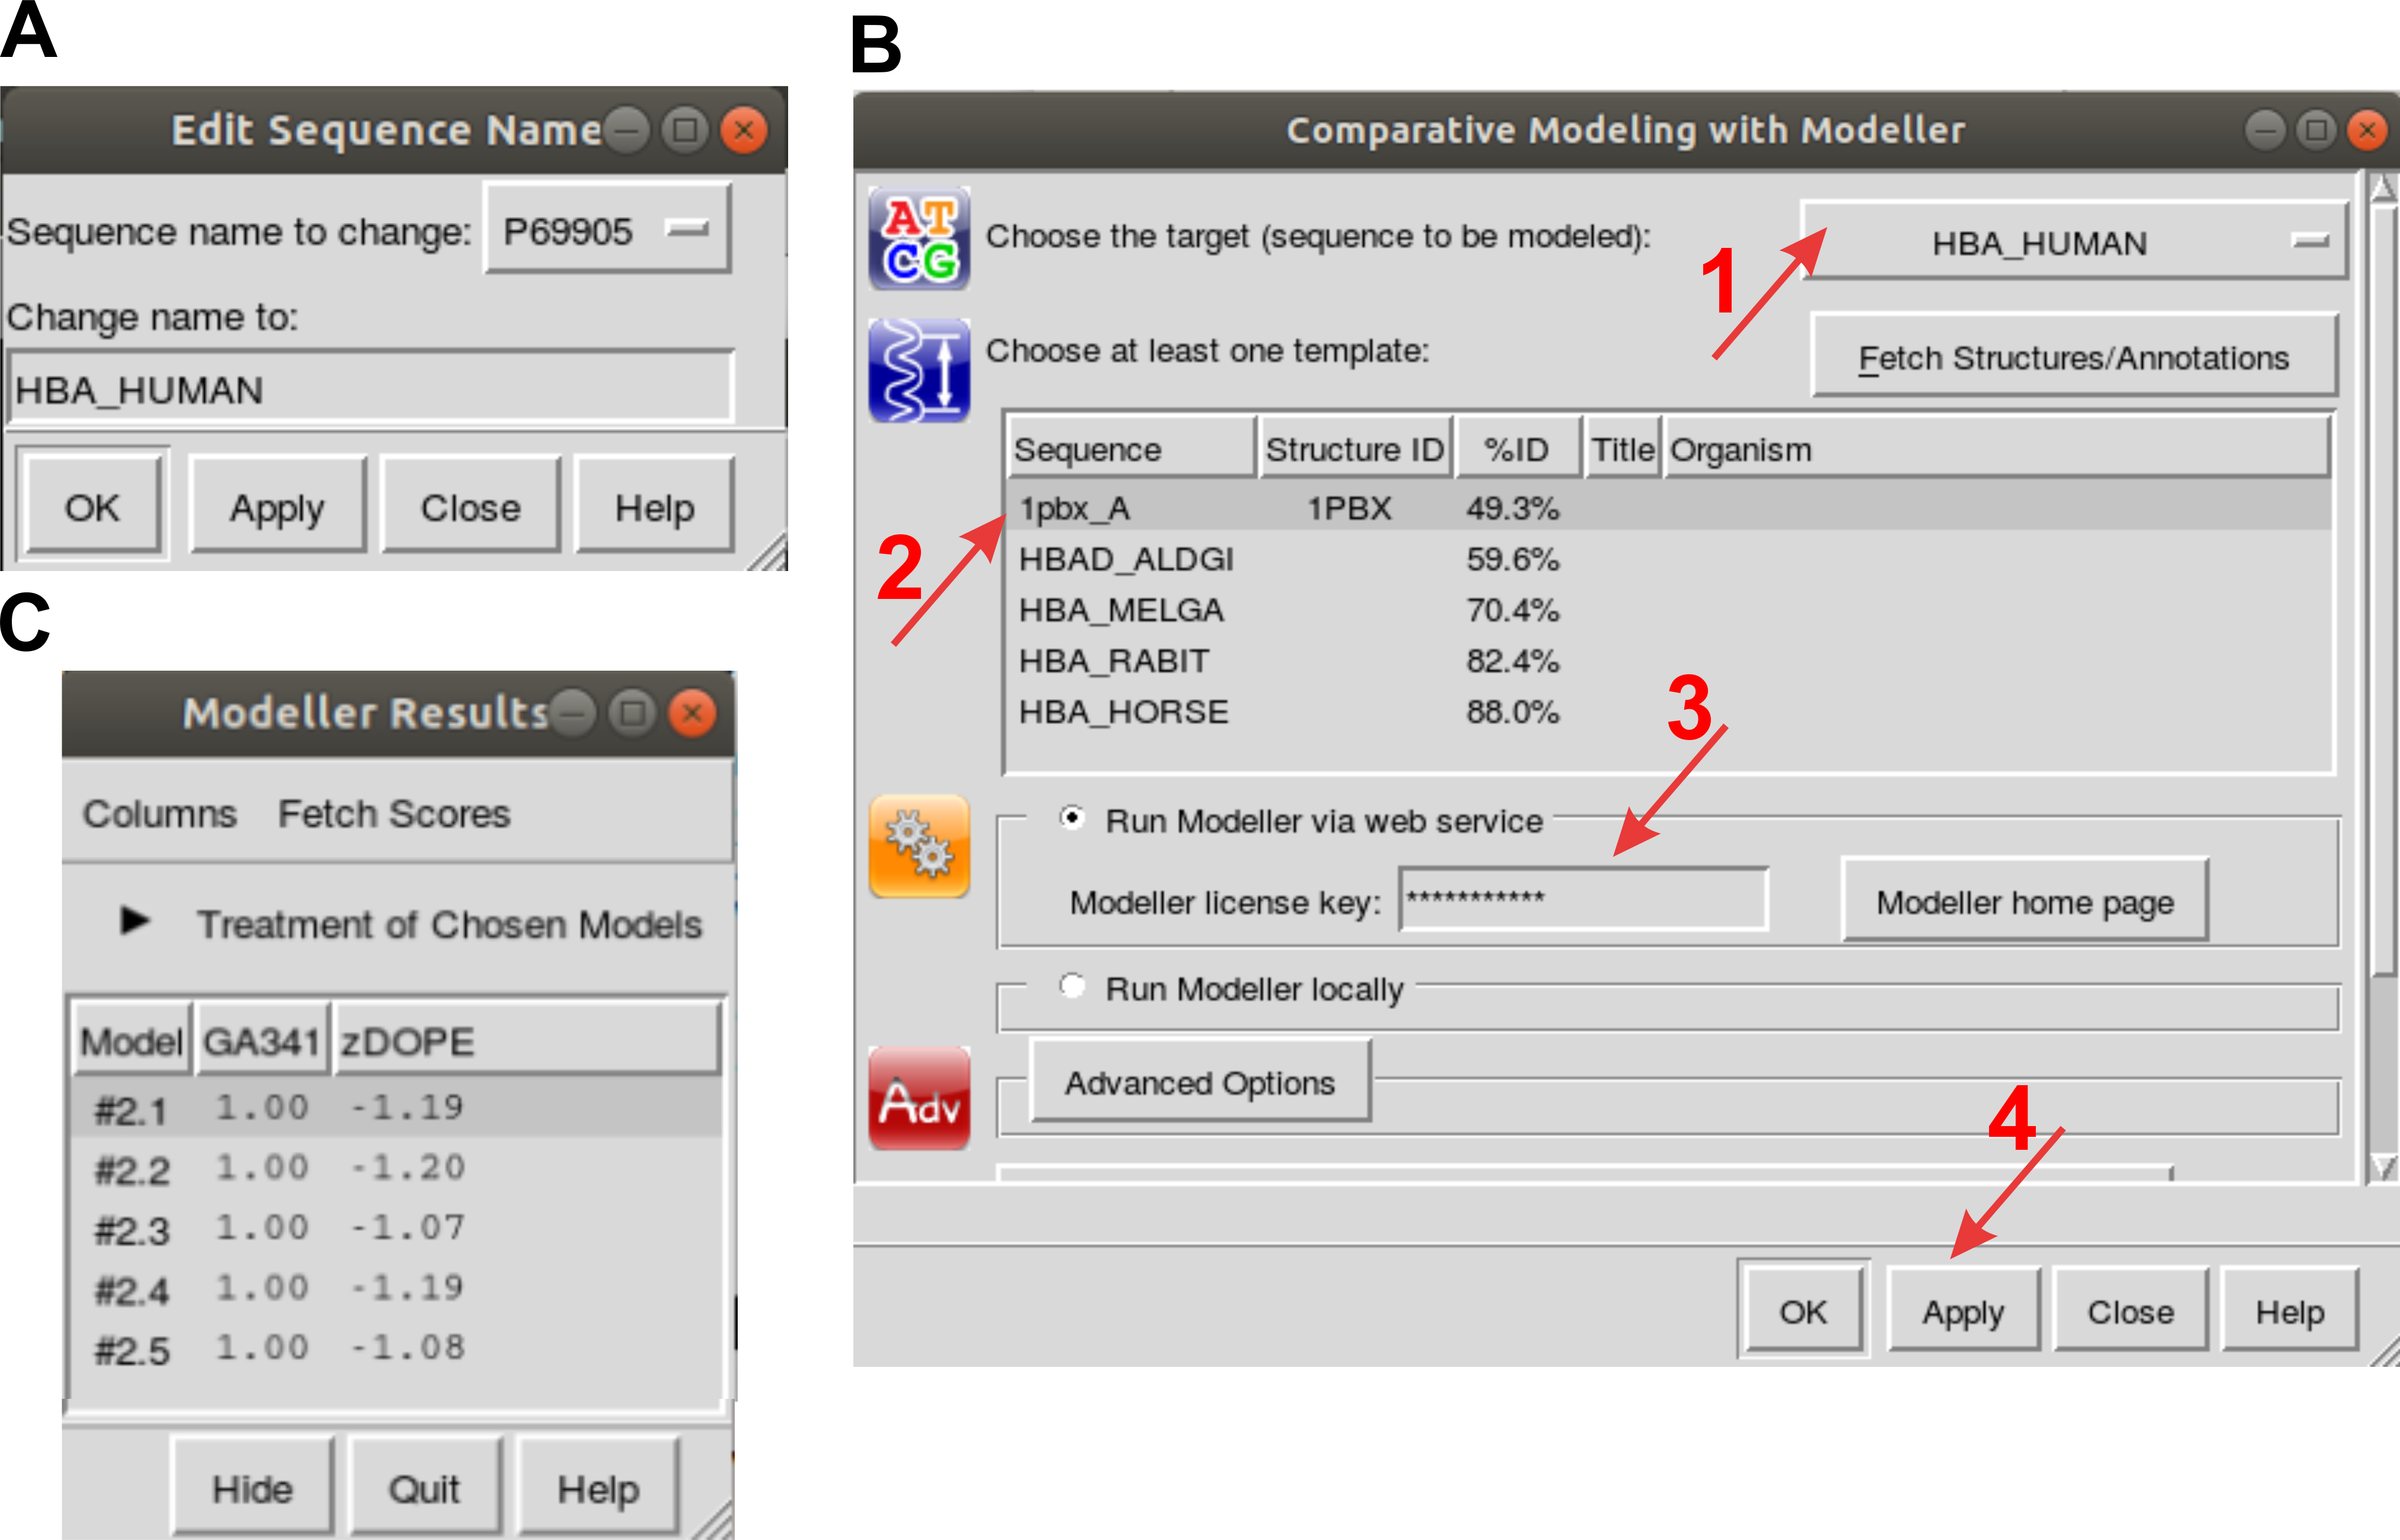
\includegraphics[width=0.80\textwidth]{Images/Fig15}
  \caption{(A) Sequence edition. (B) Completing the form to access to homology modeling with $Modeller$. (C) Resulting \iii{models}.}
  \label{fig:modeller}
  \end{figure}
 
 Comparing your selected \iii{model} of human \ttt{metHgb} $\alpha$ subunit with \ttt{1PBX\_A} \iii{template}, we observe that the selected \iii{model} \ttt{\#2.1} does not contain the \ttt{HEME} prosthetic group (\ffigure{fig:chimera_model} (A)). Before saving the \iii{model}, the \iii{template} \ttt{HEME} group will thus be added to your \iii{model} in $Chimera$. With this aim, open $Chimera$'s command line; from $Chimera$ main menu (\ttt{Favorites -> Command Line}) and delete every atom of \ttt{1PBX} \iii{template}, except the \ttt{HEME} group associated to chain \ttt{A}. To preserve residue 144 (\ttt{HEME} group) in chain \ttt{A}, write the next command line (\ffigure{fig:chimera_model} (A)(1)):\\ 
 
 \ttt{delete \#1:0-143.A, 145-.A, .B}\\ or\\
 \ttt{delete \#1:0-143.A}\\ \ttt{delete \#1:145-.A}\\ \ttt{delete\#1:.B}\\
 
 Go to the Model Panel and select models \ttt{\#1} and \ttt{\#2.1} simultaneously, then press \ttt{Copy/Combine} on the right side column (\ffigure{fig:chimera_model} (B)(2)). Model Panel shows the new \iii{model} created \ttt{\#3} (3), that we can save in the command line (4) writing:\\
 
 \ttt{scipionwrite model \#3}\\
 
 \begin{figure}[H]
  \centering 
  \captionsetup{width=.7\linewidth} 
  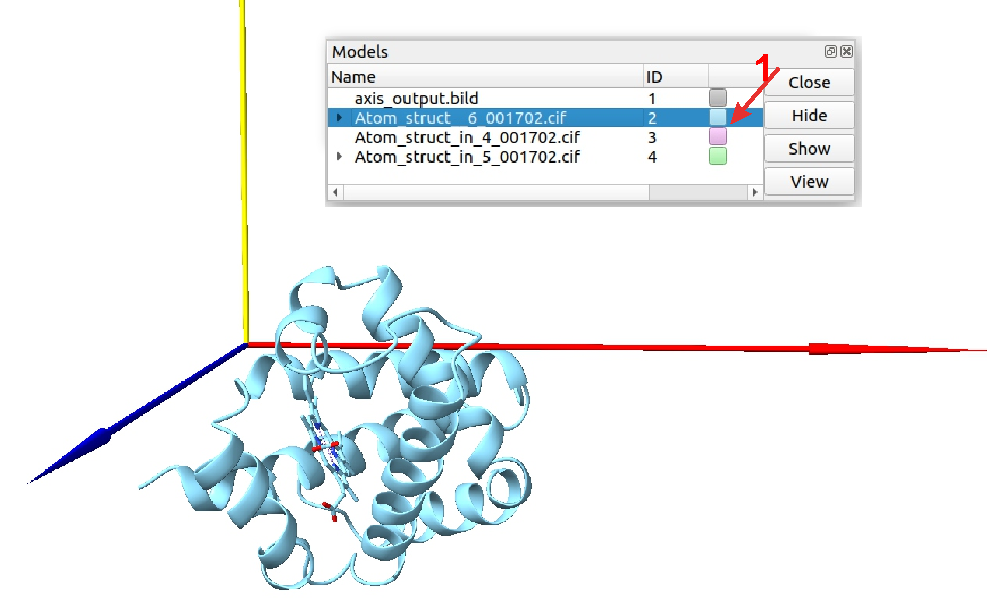
\includegraphics[width=0.80\textwidth]{Images/Fig16}
  \caption{\iii{Model} selection in $Chimera$. (A) Selected \iii{model} \ttt{\#2.1}. (B) Creation of full final \iii{model} of human \ttt{metHgb} $\alpha$ subunit, including \ttt{HEME} group.}
  \label{fig:chimera_model}
  \end{figure}
 
 After closing $Chimera$, you can visualize (\ffigure{fig:model_from_template_protocol} (8)) your full predicted \iii{model}. In a similar process, you can also obtain human \ttt{metHgb} $\beta$ subunit. Remark that in this case, the \ttt{HEME} group will be kept with the next $Chimera$ command line: \\
 \ttt{delete \#1:.A, 0-147.B, 149-.B}\\ or \\
 \ttt{delete \#1:.A}\\ \ttt{delete \#1:0-147.B}\\ \ttt{delete \#1:149-.B}\\
  
If for any reason you decide to go back and check a different \iii{model} from the five \iii{models} initially provided by $Modeller$, you can do it by using \scommand{chimera restore session} protocol (Appendix \ref{app:chimeraRestoreSession}). This protocol is allowed to be used whenever $Chimera$ session had been saved, specifically after using protocols $Chimera$ \ttt{rigid fit}, $Chimera$ \ttt{operate}, and \scipion \ttt{model from template}. In addition to the $Chimera$ command line \ttt{scipionss}, command line \ttt{scipionwrite} also save $Chimera$ session by default. So, if you want to restore a previous session just open the form (\ffigure{fig:restore_session_protocol}, 1), and include the session that you'd like to restore (2).

 \begin{figure}[H]
  \centering 
  \captionsetup{width=.7\linewidth} 
  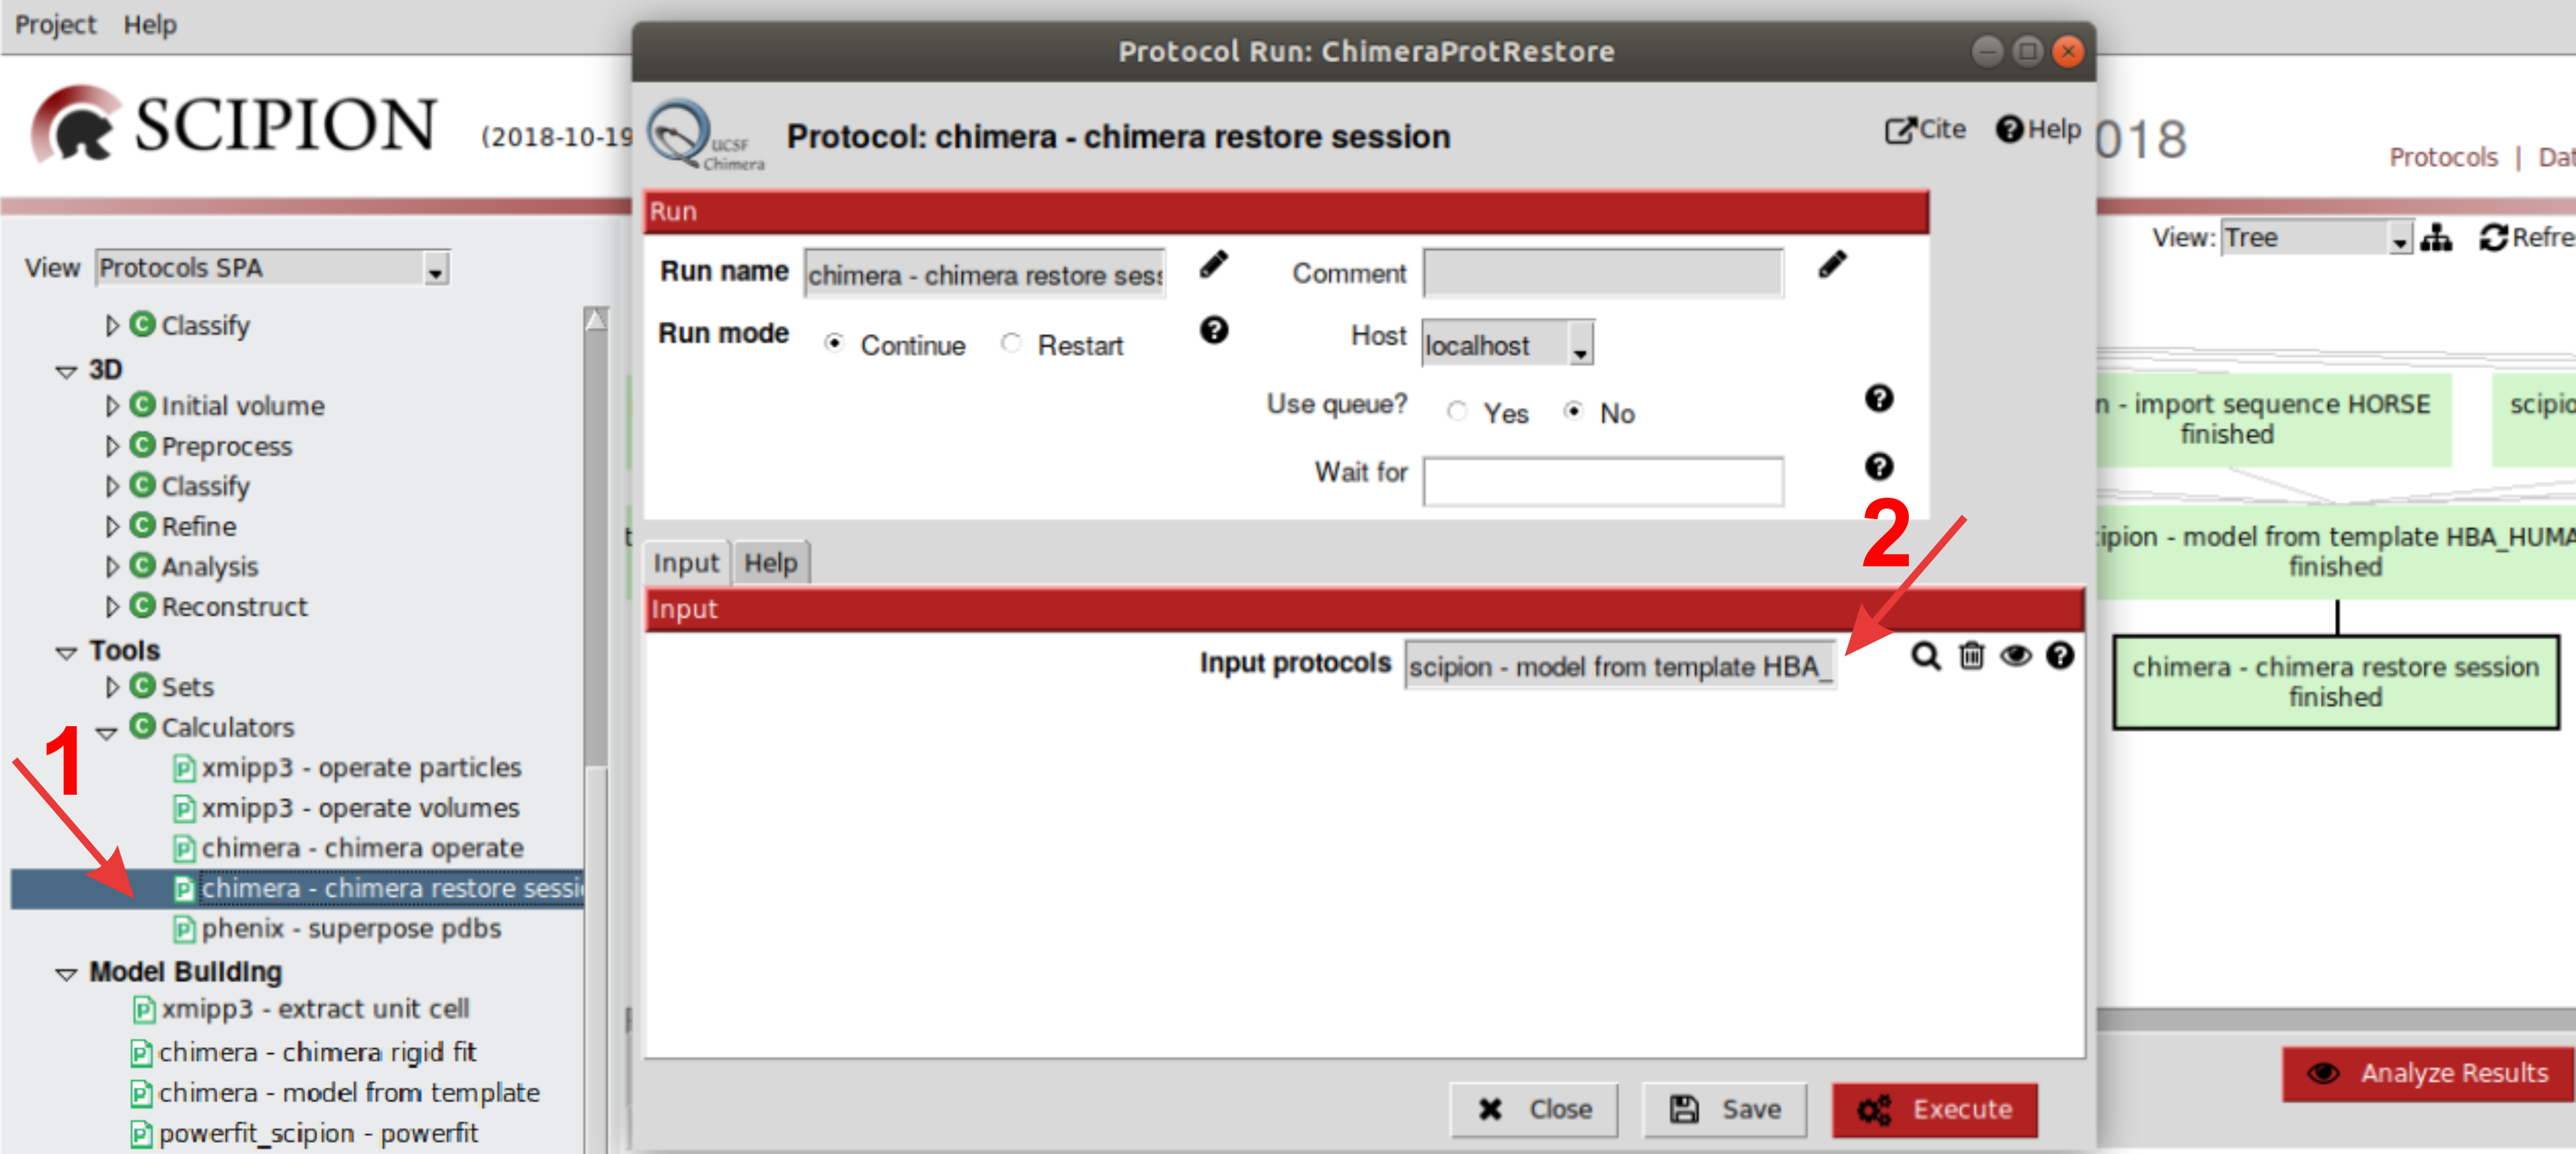
\includegraphics[width=0.90\textwidth]{Images/Fig17}
  \caption{Restoring session in $Chimera$.}
  \label{fig:restore_session_protocol}
  \end{figure}
%%%
\section{Merging 3D Maps and Atomic Structures: Rigid Fitting}
Once we have the predicted \ttt{model} of any structural element included in our map, fitting that \ttt{model} in the volume constitutes the next step in the modeling workflow. Two protocols have been included in \scipion with this purpose, \scommand{powerfit} (Appendix \ref{app:powerfitProtocol}, \citep{vanzundert2016}) and \scommand{chimera rigid fit} (Appendix \ref{app:chimeraRigidFit}). The first one allows automatic fitting of models in maps, while the second one only does it when model and map are quite close, thus requiring manual fitting in advance. Although there is no a general rule to fit map and model, because it will depend on the particular problem and on our previous knowledge, in this tutorial we are going to use \powerfit application first, followed by the final \ttt{Fit in Map} in \chimera \ttt{rigid fit}. In our experience \powerfit performance decays for large 3D maps or when fitting atomic models that cover a small region of the 3D map.

\subsection*{Initial rigid fit with \powerfit}
 Open \scommand{powerfit} protocol ((\ffigure{fig:powerfit_protocol} (1)), and complete the form with the \iii{model} of atomic structure previously saved in \chimera (2), the extracted unit cell volume (3), and volume resolution (4). Among the advanced parameters, consider carefully the angular step (5) according to the size of your volume and your computing power. Despite getting a more accurate result, fitting of large volumes takes more time as  lower values of angular step are requested.  
 
 \begin{figure}[H]
  \centering 
  \captionsetup{width=.7\linewidth} 
  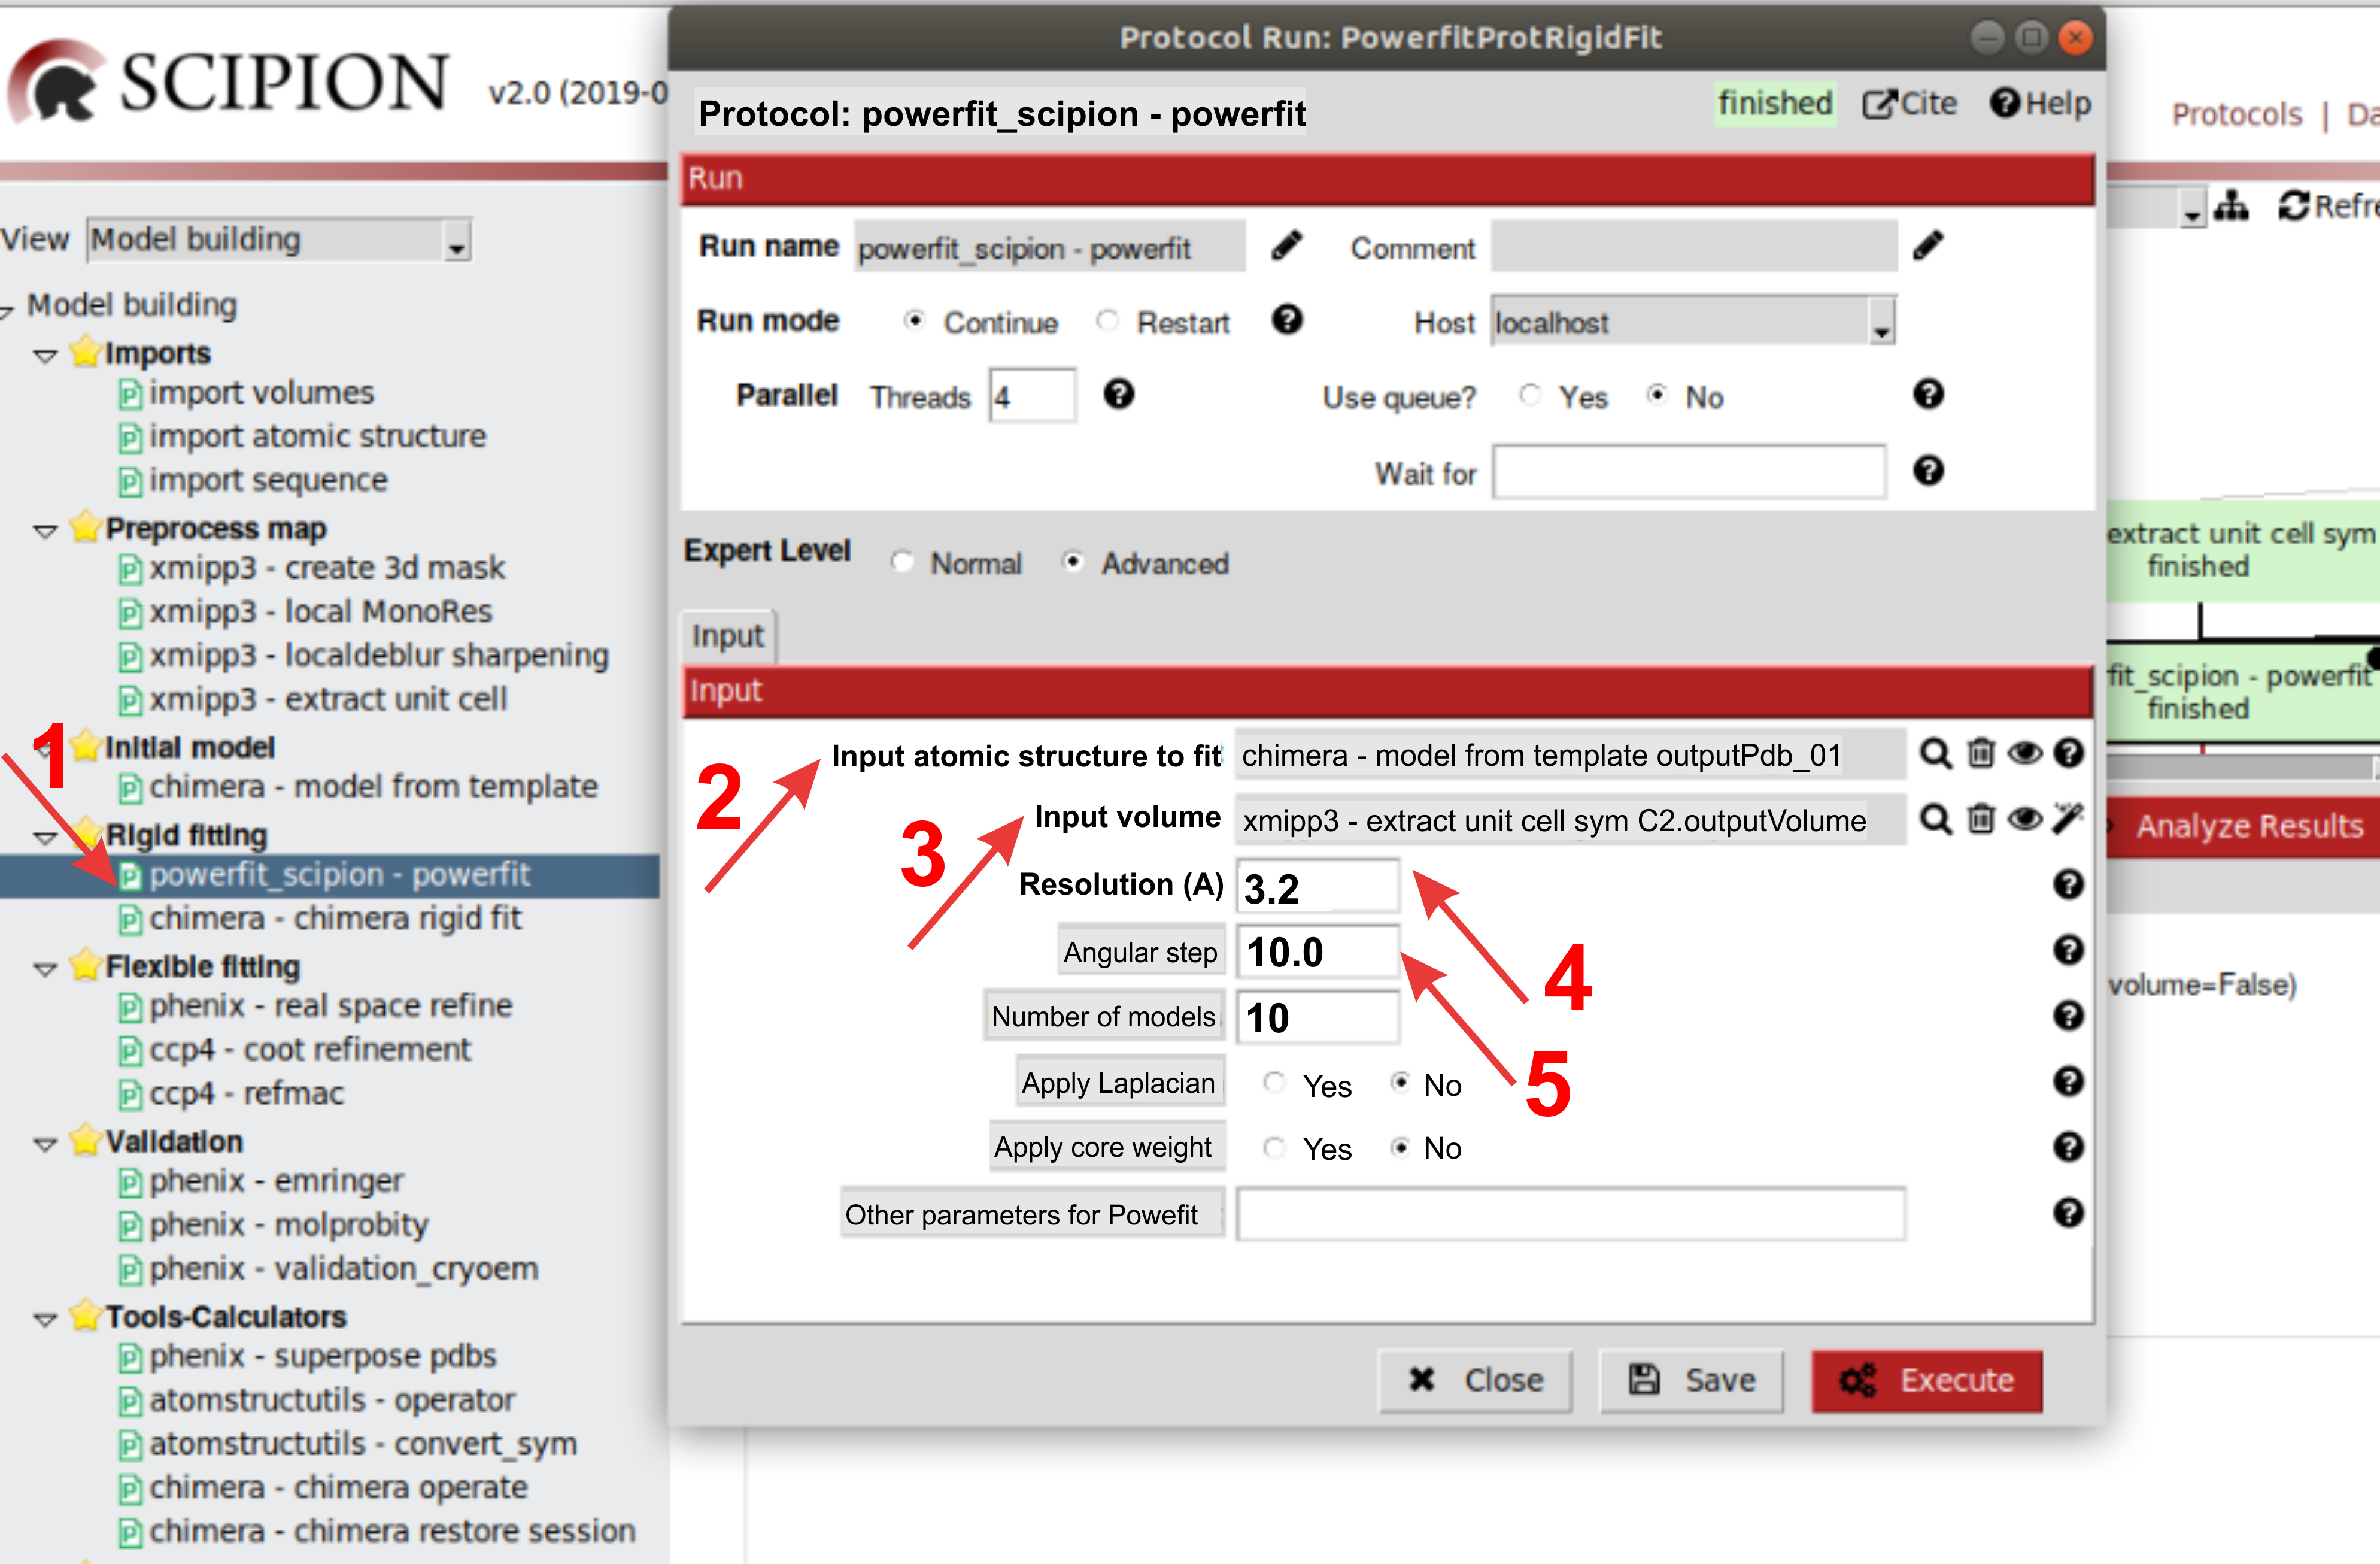
\includegraphics[width=0.85\textwidth]{Images/Fig18}
  \caption{Rigid fit with \powerfit: Filling in the protocol form.}
  \label{fig:powerfit_protocol}
  \end{figure}
 
 After executing the \scommand{powerfit} protocol, you can check results ((\ffigure{fig:powerfit_results_table} (A)(1)). The first table opened allows you to check the fitting quality (2) of best score-ordered fits in a second table (B). In our example only two fits are proposed. You can check which one fits better to the map by writing the selected fit number in the \ttt{Model to visualize} square window, and then displaying the fitting (3).
 
 \begin{figure}[H]
  \centering 
  \captionsetup{width=.7\linewidth} 
  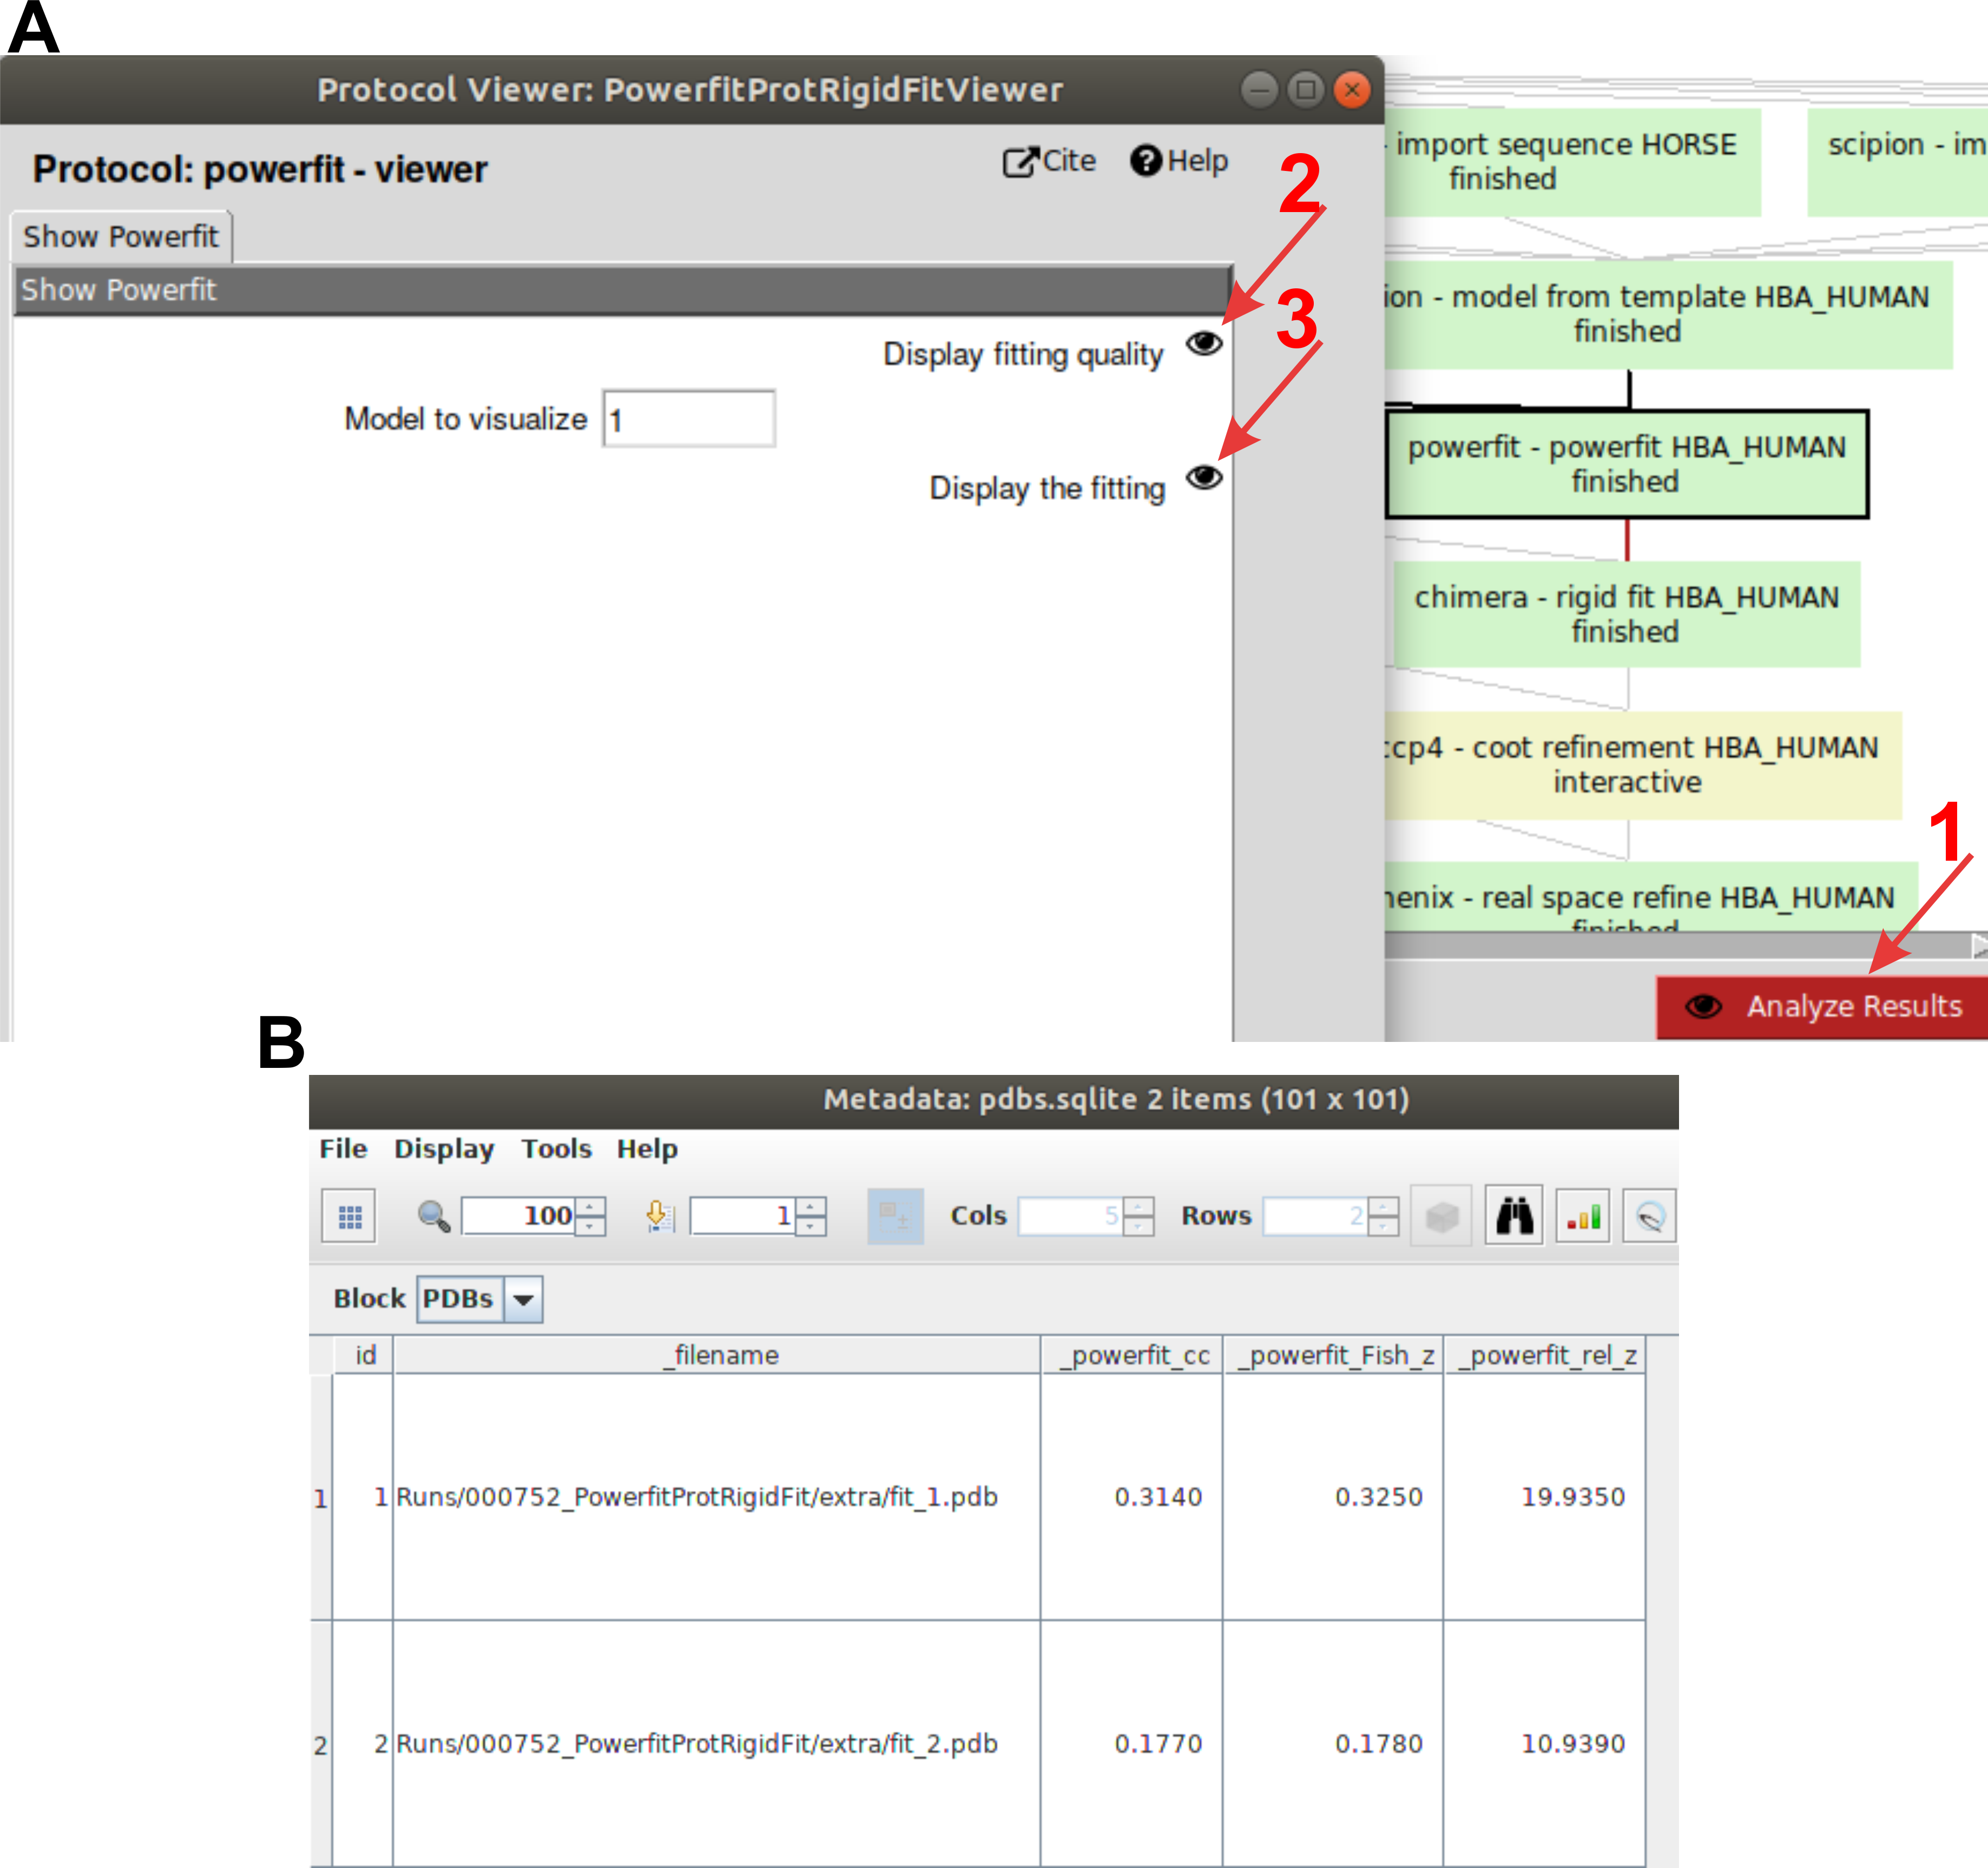
\includegraphics[width=0.85\textwidth]{Images/Fig19}
  \caption{Rigid fit with \powerfit: Checking results by score.}
  \label{fig:powerfit_results_table}
  \end{figure}
  
  \ffigure{fig:powerfit_results_figs} shows the fitting of the two possible fits between map and \ttt{models} posed by \powerfit (\ttt{fit\_1.pdb}, A, and \ttt{fit\_2.pdb}, B, green- and pink-colored, respectively). Although both of them seem to fit quite well the extracted unit cell map, only one of them should be OK. The other $model$ one must misfit the volume area that corresponds to \ttt{metHgb} $\beta$ subunit. This anomalous behavior of our \iii{model} is not surprising because \ttt{Hgb} $\alpha$ an $\beta$ subunits are 42.86\% sequence identical. 
  
 \begin{figure}[H]
  \centering 
  \captionsetup{width=.7\linewidth} 
  \includegraphics[width=0.85\textwidth]{Images/Fig20}
  \caption{Rigid fit with \powerfit: Checking the best fits in \chimera.}
  \label{fig:powerfit_results_figs}
  \end{figure}
  
 \subsection*{ Completing rigid fit with \chimera \ttt{rigid fit}}
 
 In order to assess which one of the structures fits the map better, the fitting has to be improved with \scommand{chimera rigid fit} protocol. Open this protocol (\ffigure{fig:chimera_rigid_fit} (1)), include the extracted unit cell as volume (2), one of the structures fitted (3), the other one (4), and execute the protocol.
 
 \begin{figure}[H]
  \centering 
  \captionsetup{width=.7\linewidth} 
  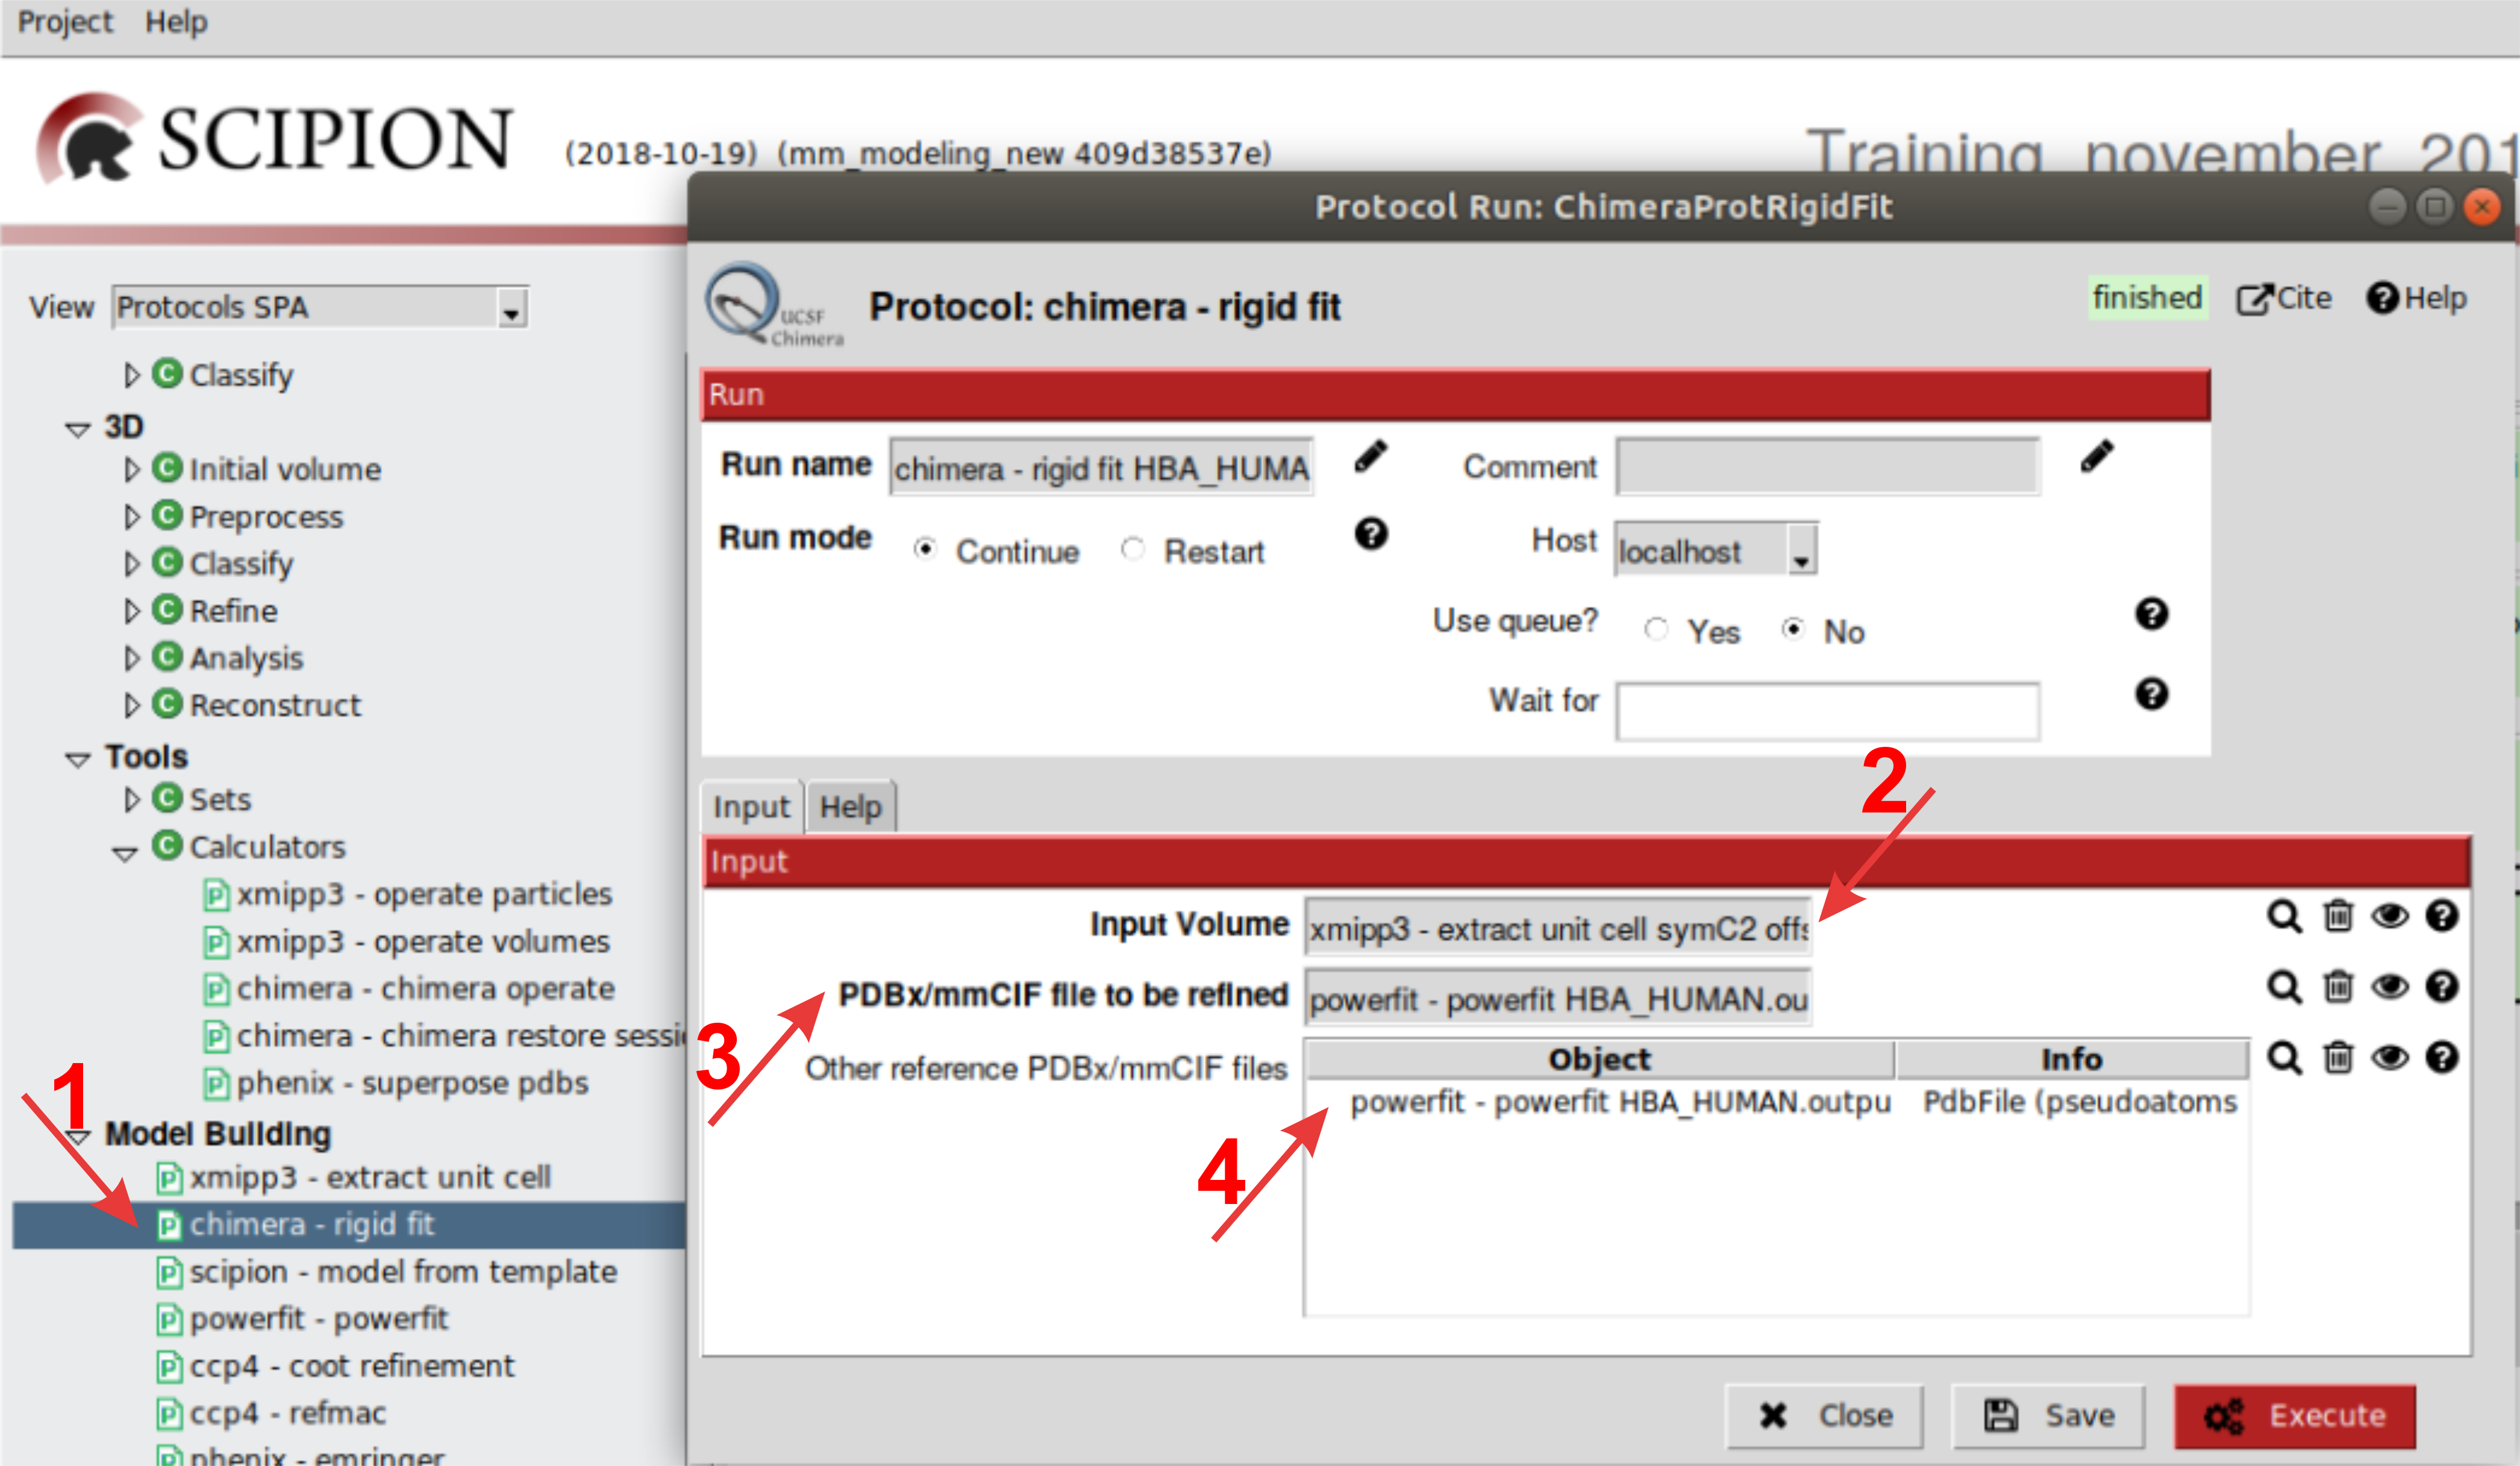
\includegraphics[width=0.85\textwidth]{Images/Fig21}
  \caption{Completing the \chimera rigid fit protocol form.}
  \label{fig:chimera_rigid_fit}
  \end{figure}
  
  Once opened \chimera graphical window, select in the upper main menu \ttt{Tools -> Volume Data -> Fit in Map}. A small window will be opened. Select each one of the fits in \ttt{Fit} and press \ttt{Fit} to allow the automatic rigid fitting. At the lower right side of \ffigure{fig:chimera_fit_in_map}, respective windows of \ttt{Fit in map} for \ttt{fit\_1.pdb} and \ttt{fit\_2.pdb} are detailed. In spite that the amount of \ttt{atoms outside the contour} is higher in \ttt{fit\_1.pdb} than in \ttt{fit\_2.pdb}, we can not conclude that the second fitting is better than the first one, because the \ttt{Average map value} is also lower. Visual inspection of both fits should identify the appropriate fitting of \iii{model} in map.
  
  \begin{figure}[H]
  \centering 
  \captionsetup{width=.7\linewidth} 
  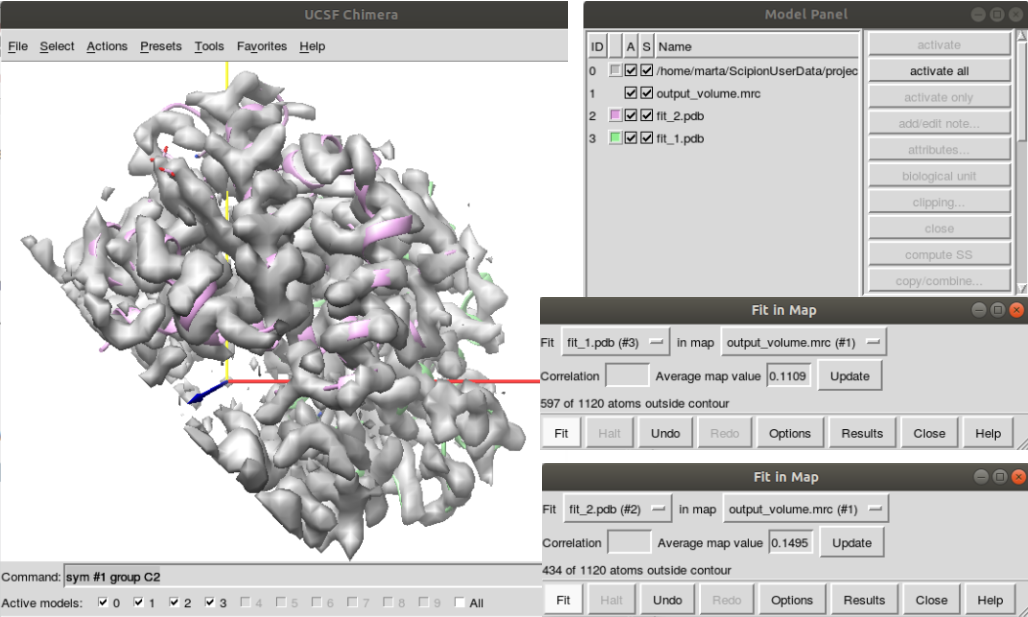
\includegraphics[width=0.85\textwidth]{Images/Fig22}
  \caption{Fitting in map with \chimera.}
  \label{fig:chimera_fit_in_map}
  \end{figure}
   
  As suggestion, before starting the visual inspection in \chimera, check first the parts of the structure that could differ the most between \ttt{metHgb} $\alpha$ and $\beta$ subunits. These divergent parts can be identified by performing an additional alignment including the $\beta$ subunit sequence. Possible steps to perform this multiple alignment: (1) import the  \ttt{metHgb} $\beta$ sequence (UnitProt id=P68871), (2) copy the protocol \scommand{model from template} and (3) add the  \ttt{metHgb} $\beta$ in the field \ttt{other sequences to align}. \ffigure{fig:multiple_alignment_HBB} shows the result of incorporating the $\beta$ subunit sequence (in yellow) to the alignment shown in \ffigure{fig:chimera_alignment}. Two regions that contain gaps of sequence are remarked in red frames. The first one, involving residues 19 and 20, absent in $\beta$ subunit, and the second one, after residue 51, could be the most relevant to differentiate between subunits. Look at them and identify the correct fit. You can highlight those residues in \chimera writing in the command line:\\
  \ttt{sel :19-20}\\
  \ttt{sel :50-55}
  
  \begin{figure}[H]
  \centering 
  \captionsetup{width=.7\linewidth} 
  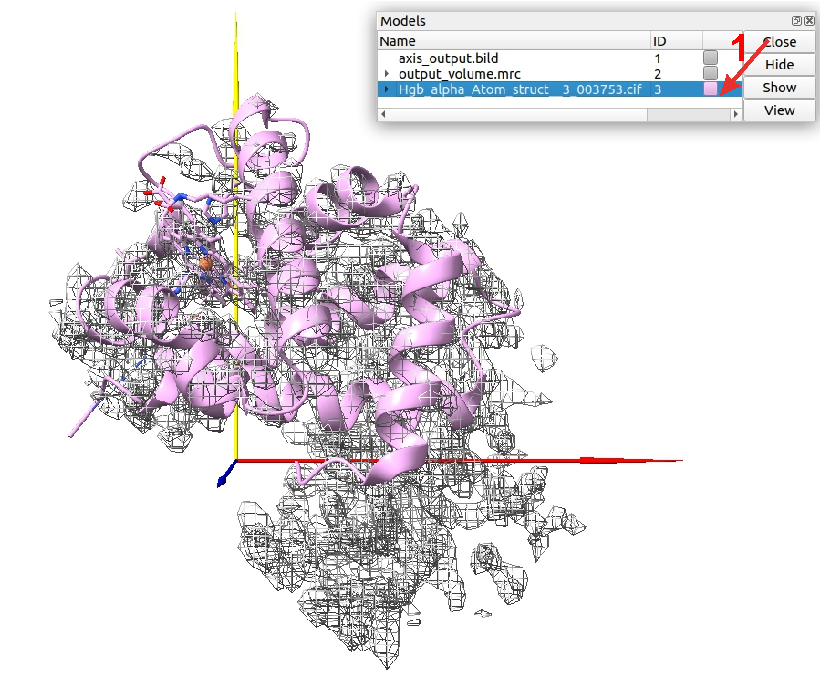
\includegraphics[width=0.85\textwidth]{Images/Fig23}
  \caption{Multiple sequence alignment including \ttt{Hgb} $\beta$ subunit (\ttt{HBB\_HUMAN}).}
  \label{fig:multiple_alignment_HBB}
  \end{figure}
  
  Once identified the appropriate fit, you can save it as fitted $model$ of the \ttt{metHgb} $\alpha$ subunit. Replacing \ttt{n} by your $model$ number (\ttt{1}, \ttt{2}), write in the command line of \chimera graphical window:\\
  
  \ttt{scipionwrite model \#n refmodel \#1 saverefmodel 0}\\
  
In case you are still unable to decide which one is the best fit, don't worry. You will make your mind up with the next step in the workflow, but then save both fits with \ttt{scipionwrite} \chimera command line. Don't forget to change the $model$ number. Your fitted models will be saved by \chimera with names \ttt{chimeraOut0001.pdb} and \ttt{chimeraOut0002.pdb}.
 

\section{Refinement: Flexible fitting}
\label{refinementFlexibleFitting}
Although the rigid fitting approximates map and atomic $model$, a detailed visual inspection of map and model reveals that part of residues are not perfectly fitted. In order to get a better fit, not only of the carbon skeleton but also of residue side chains, a flexible fitting or refinement has to be accomplished. Refinement can thus be defined as the optimization process of fitting $model$ parameters to experimental data. Different strategies can be followed, that can be categorized as refinement in the real space and refinement in Fourier space. Implemented in \scipion are two protocols for real space refinement, \scommand{ccp4 - coot refinement} (Appendix \ref{app:ccp4CootRefinement}, \citep{emsley2010}) and \scommand{phenix - real space refine} (Appendix \ref{app:realSpaceRefineProtocol}, (\citep{afonine2018}), and one protocol to refine in reciprocal space, \scommand{ccp4 - refmac} (Appendix \ref{app:ccp4Refmac}, \citep{vagin2004}).

 \subsection*{CCP4 \coot Refinement}
 
 Initially devoted to atomic models obtained by X-ray crystallography methods, \coot (from Crystallopgraphic Object-Oriented Toolkit) is a 3D computer graphics tool that allows simultaneous display of map and fitted $model$ to accomplish mostly interactive modeling operations. Although this tutorial does not try to show every functionality of \coot, but indicate how to open, close and save partial and final \coot refined structures in \scipion, some of \coot basic relevant commands will be shown. Initially, we are going to refine our \iii{moldel} with \coot. First of all, open \scommand{ccp4 - coot refinement} (\ffigure{fig:coot_refinement_protocol} (1)), load the extracted unit cell volume (2), with electron density normalized to 1, and the fitted structure $model$ (3). Load also the second fit (4) if you are not still sure about the correct fitted structure. Reading the protocol Help is recommended. After executing the protocol (5), \coot graphics window will appear to start working. 
 
 \begin{figure}[H]
  \centering 
  \captionsetup{width=.7\linewidth} 
  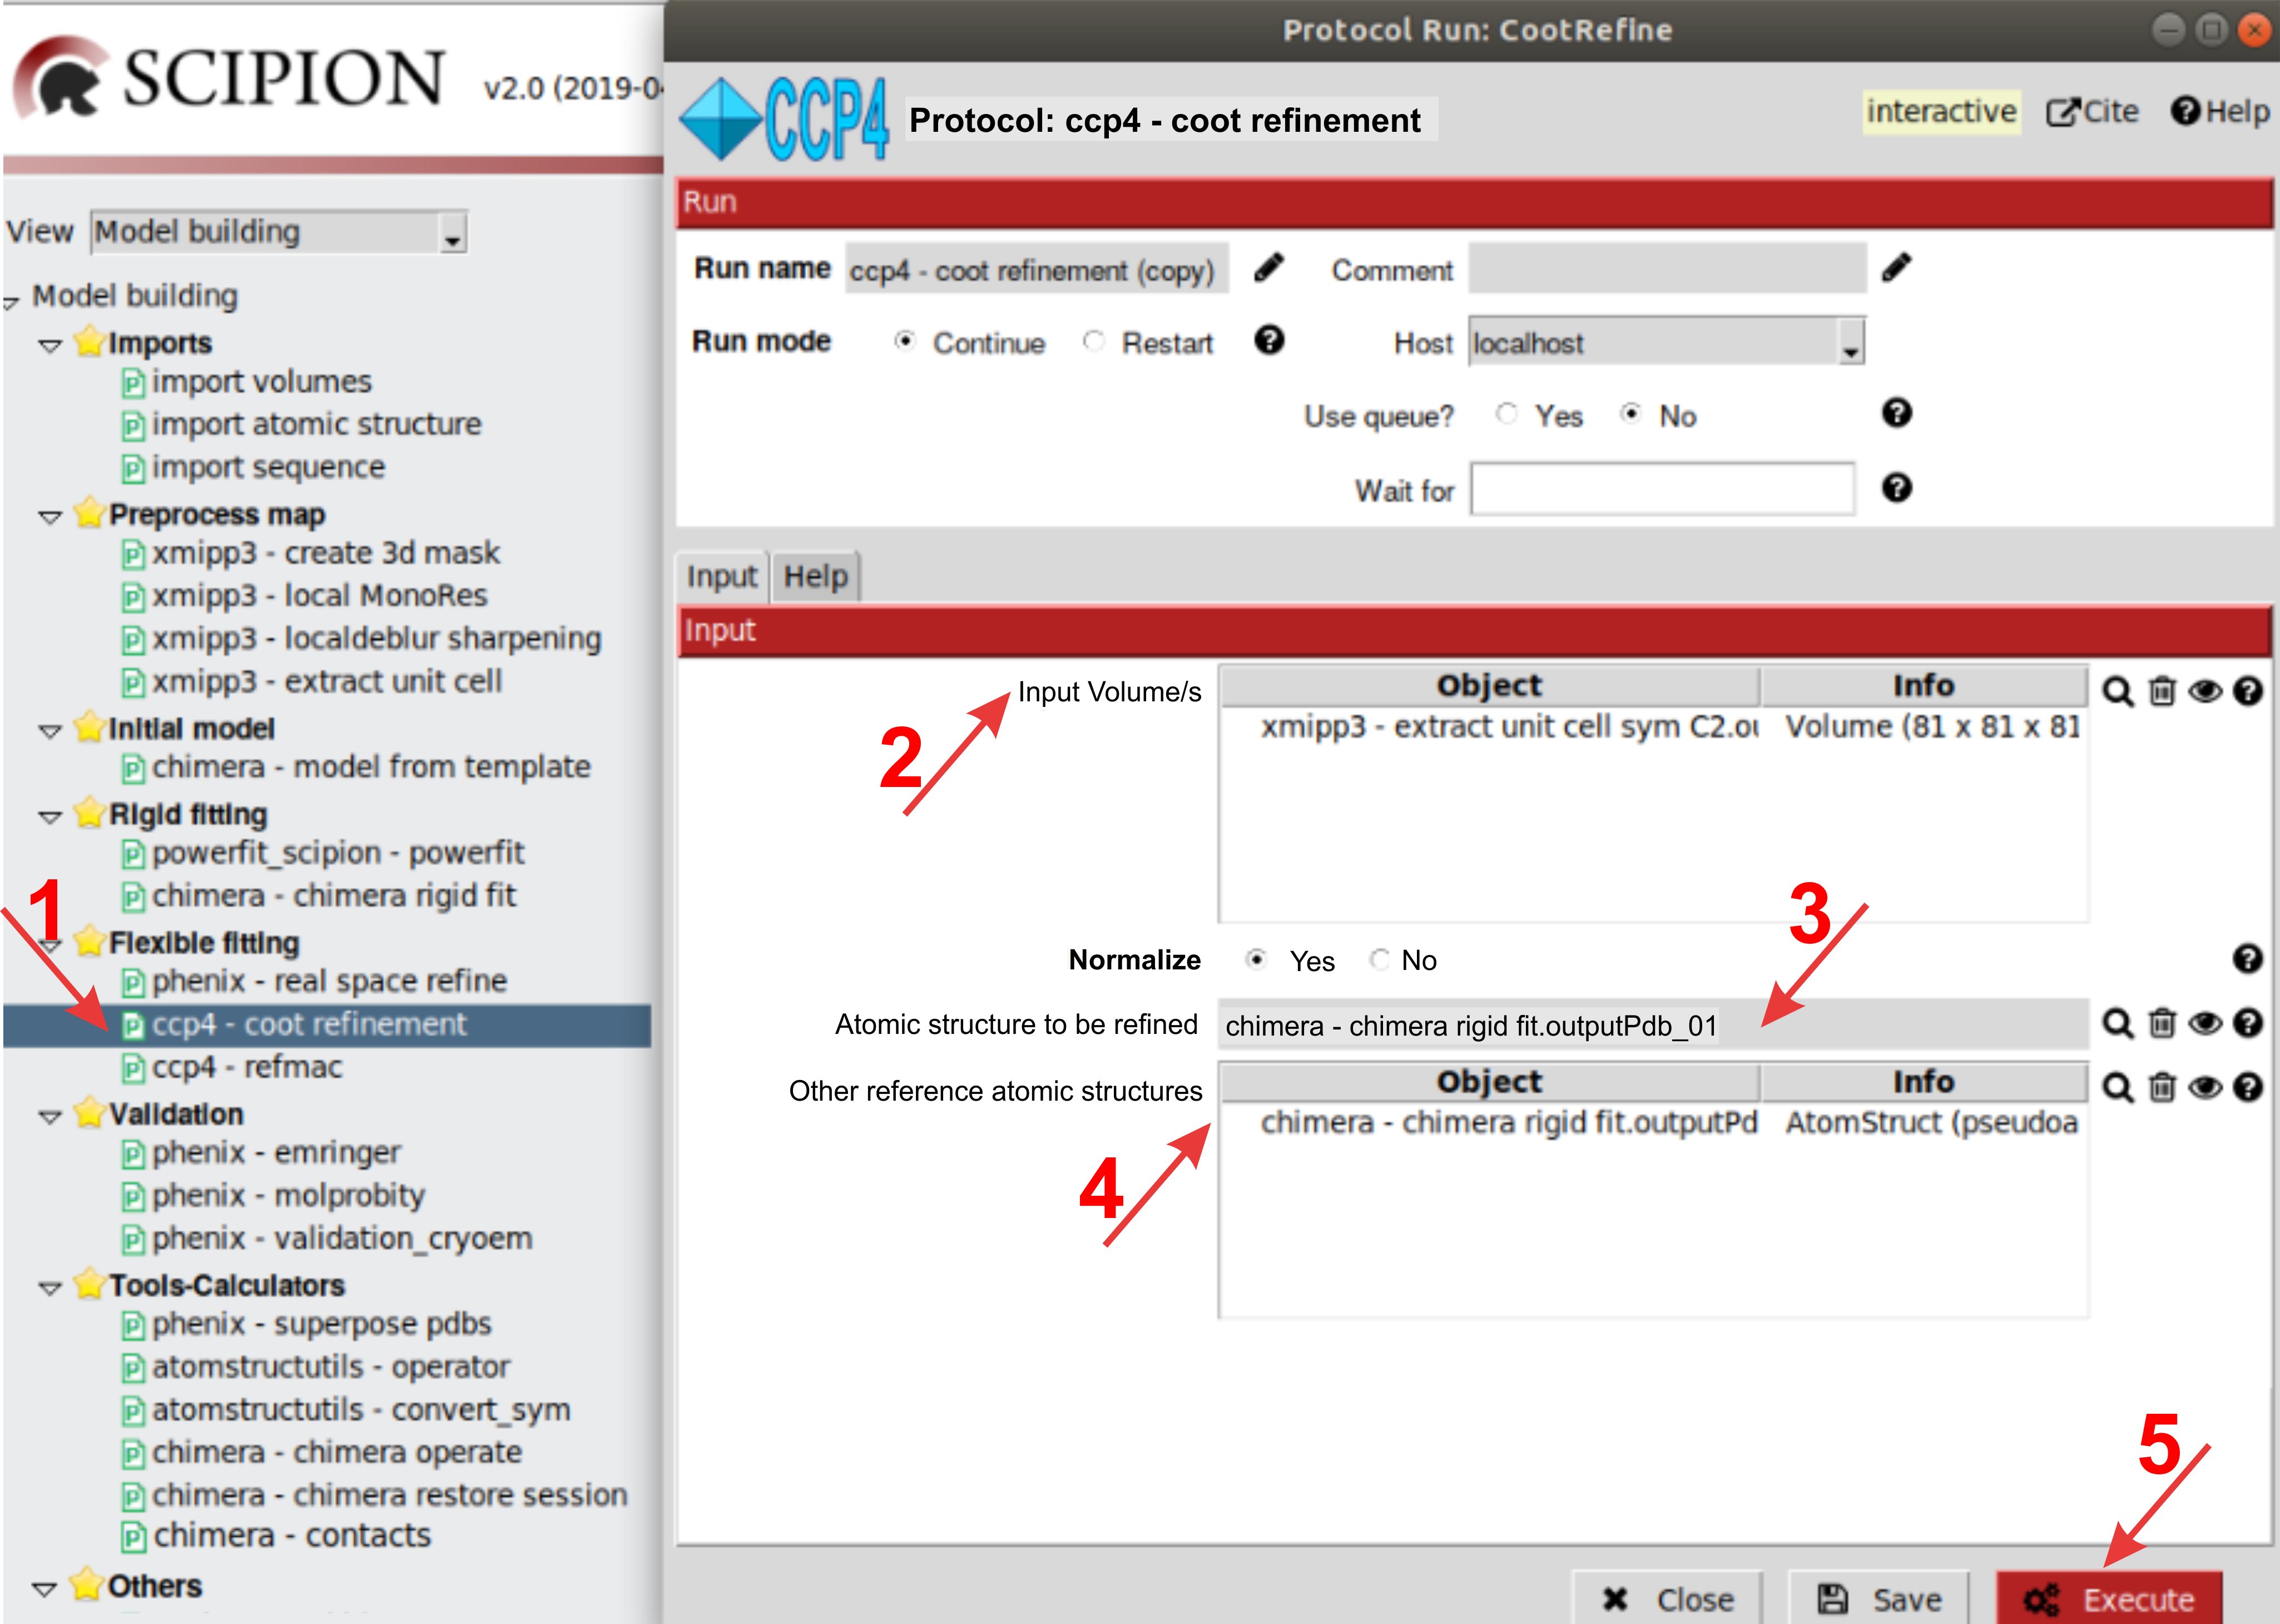
\includegraphics[width=0.85\textwidth]{Images/Fig24}
  \caption{Filling in \coot refinement protocol.}
  \label{fig:coot_refinement_protocol}
  \end{figure}
  

  To check the objects downloaded in \coot, go to the second bar of the main menu and select \ttt{Display Manager}. Map \ttt{(output\_volume.mrc)} (number \ttt{\#2}) and models \ttt{chimeraOut0001.pdb} and \ttt{chimeraOut0002.pdb} (numbers \ttt{\#1} and \ttt{\#0}, respectively) are displayed. To start, we are going to identify the faired fitted $model$ to the density map in order to delete in the \ttt{Display Manager} menu the other $model$, which is misfitted. Visual inspection would clarify this point, although direct observation of the \ttt{Density fit analysis} might be a shorter way. With this aim, go to the main menu of \coot graphical window and select \ttt{Validate -> Density fit analysis}. This density analysis is compared for the two possible fitted \iii{models} in \ffigure{fig:coot_density_fit_analysis}. As you can see, model \ttt{chimeraOut0001.pdb} shows that residues 19, 20 and 22, framed in \ffigure{fig:multiple_alignment_HBB}, do not fit to the density map, as expected from the misfit of the $\alpha$ subunit in the density of the $\beta$ subunit.
 
 \begin{figure}[H]
  \centering 
  \captionsetup{width=.7\linewidth} 
  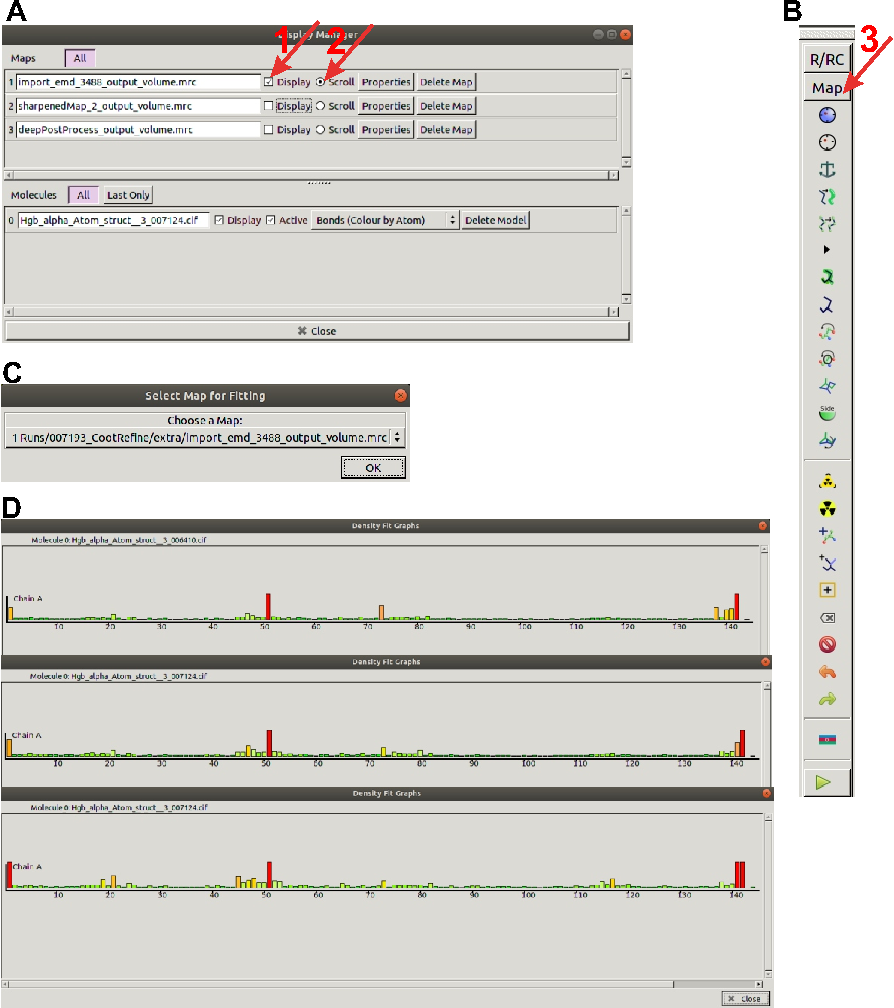
\includegraphics[width=0.85\textwidth]{Images/Fig25}
  \caption{\coot comparison of \iii{model} fit in the map density.}
  \label{fig:coot_density_fit_analysis}
  \end{figure}
  
  Go again to \ttt{Display Manager} and delete the \iii{model} \ttt{chimeraOut0001.pdb} pressing \ttt{Delete Model}. From now ahead, the \iii{model} \ttt{chimeraOut0002.pdb} will be refined in the next steps of the modeling workflow.\\
  
  Before starting the refinement, IDs of chains should be fixed. Current IDs of chains are \ttt{Chain A} and \ttt{Chain} (see \ffigure{fig:coot_density_fit_analysis}) and will be changed to \ttt{Chain HEME} and \ttt{Chain A}, respectively. This can be carried out going to main \coot menu and selecting \ttt{Edit -> Change Chain IDs}. Verify the identity of your \iii{model} molecule (\ffigure{fig:coot_change_name_ID} (1), select the initial Chain ID (2, 4), and write the new Chain ID (3, 5). Finally, press \ttt{Apply New Chain ID}.
 
 \begin{figure}[H]
  \centering 
  \captionsetup{width=.7\linewidth} 
  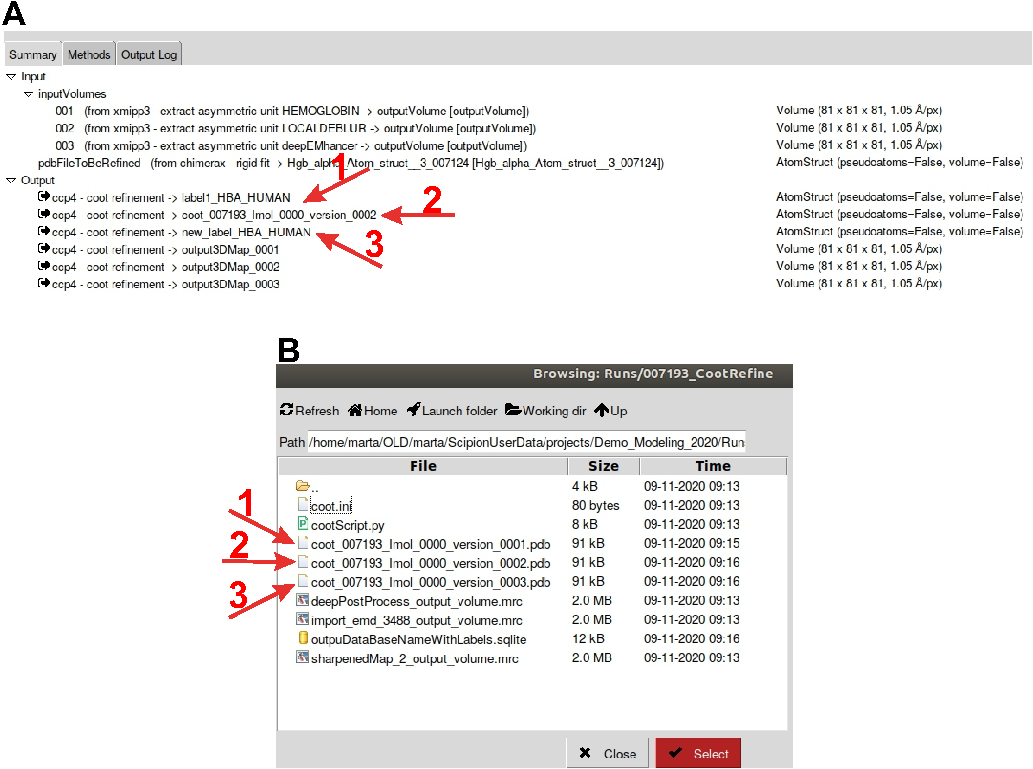
\includegraphics[width=0.85\textwidth]{Images/Fig26}
  \caption{\coot change chain ID of \iii{model} \ttt{chimeraOut0002.pdb}.}
  \label{fig:coot_change_name_ID}
  \end{figure}
  
  According to \ffigure{fig:coot_density_fit_analysis}, \ttt{MET} residue of the new chain \ttt{A} does not fit to the map density. Maybe this residue has been processed post-translationally, as we have anticipated in \textbf{Starting Input data} section. To solve this question, go to \coot main menu and select \ttt{Draw -> Go To Atom... -> Chain A -> A 1 MET} (\ffigure{fig:coot_go_to_atom} (A)). \ttt{MET} residue will be located in the center of \coot graphics widow. Check if this residue is surrounded by any electron density. As \ffigure{fig:coot_go_to_atom} (B)(1) shows, no density associates to the first chain residue. \ttt{MET} will thus be deleted. Then go to the lower right side menu and select the symbol to delete items (B)(2). Select \ttt{Residue/Monomer} in the opened \ttt{Delete item} window, and click the \ttt{MET} residue that you want to delete. Go again to \ttt{Validate -> Density fit analysis} and check that the red bar shown in \ttt{MET} residue (\ffigure{fig:coot_density_fit_analysis}) has disappeared.
  
  \begin{figure}[H]
  \centering 
  \captionsetup{width=.7\linewidth} 
  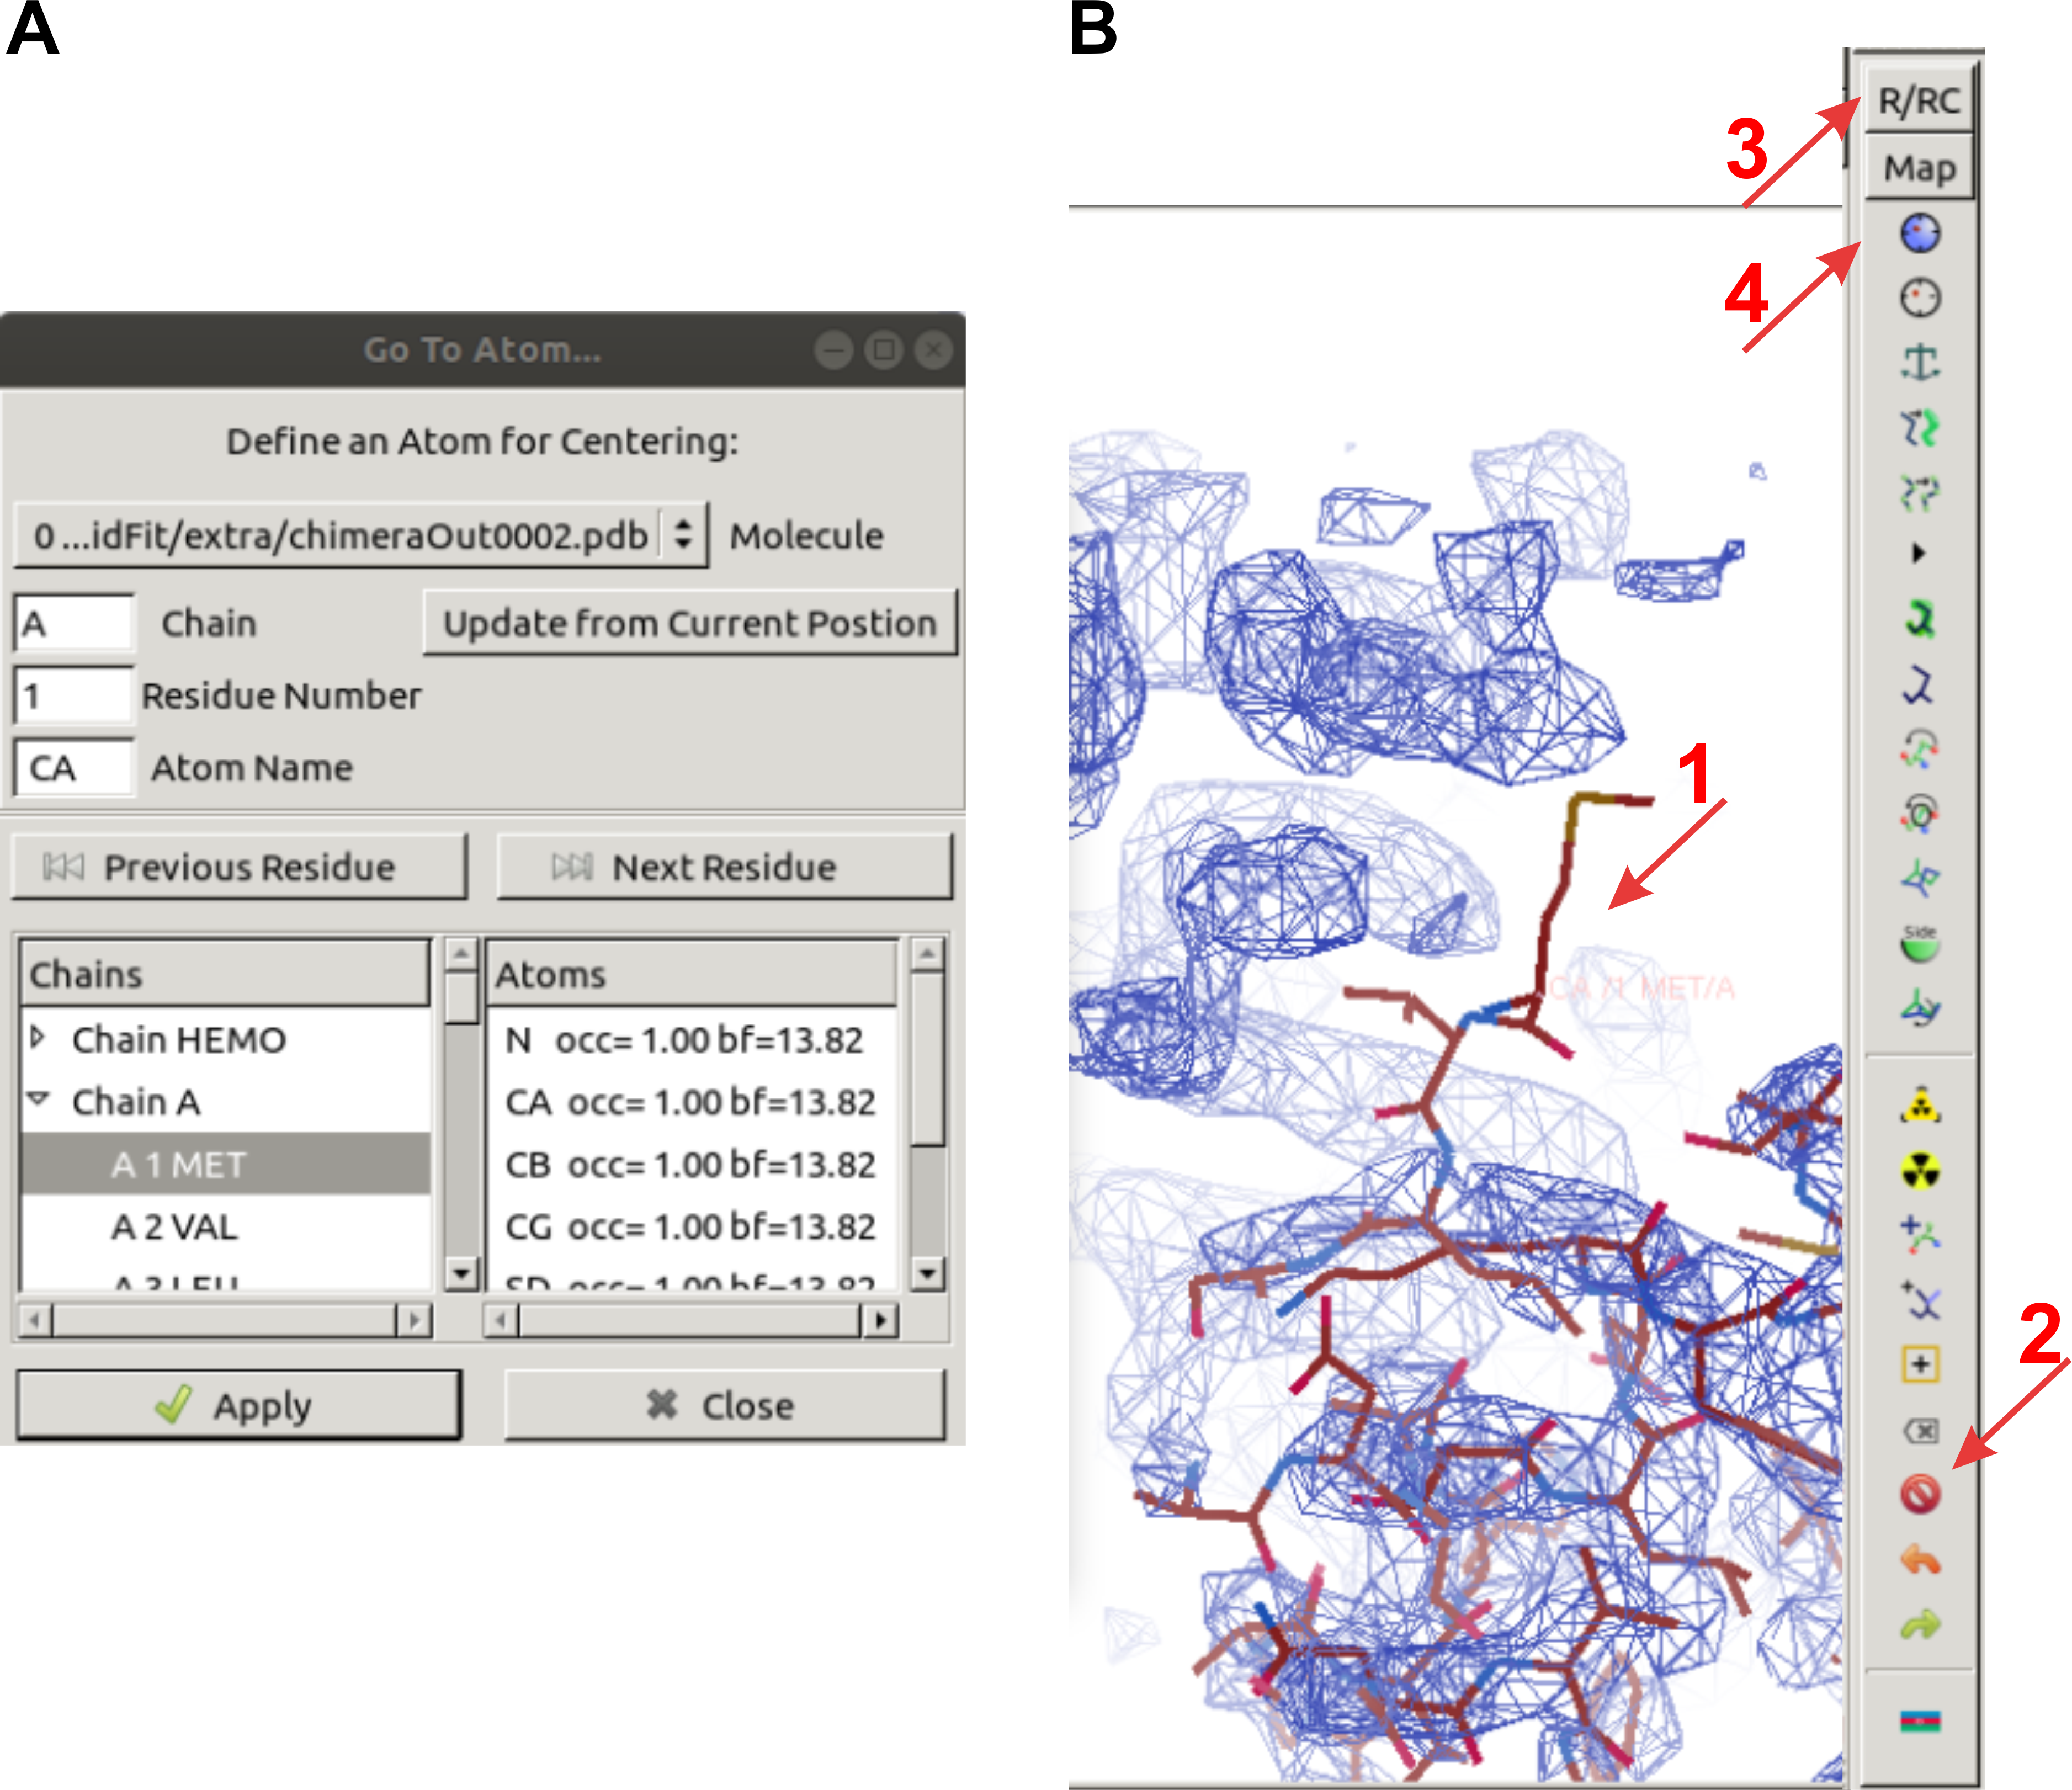
\includegraphics[width=0.80\textwidth]{Images/Fig27}
  \caption{Removing post-translationally processed Methionine residue in \coot. Note that the icons shown in the image right side may be partially hidden if the screen is small}
  \label{fig:coot_go_to_atom}
  \end{figure}
  
  Before a more detailed visual inspection of the \iii{model} fitting, an initial quick refinement may be accomplished. With this purpose, first of all, go to the upper right side menu (\ffigure{fig:coot_go_to_atom} (B)(3)) and select all four restrictions for \ttt{Regularization and Refinement} in the respective window of parameters. Secondly, open the \ttt{coot.ini} text file, 
  open \scipion browser and navigate to the ttt{extra} directory, Modify the file so it match the information shown indicated below. (See \ffigure{fig:cootini}\\
  \ttt{[myvars]}\\
  \ttt{imol: 0}\\
  \ttt{aa\_main\_chain: A}\\
  \ttt{aa\_auxiliary\_chain: AA}\\
  \ttt{aaNumber: 4}\\
  \ttt{step: 10}\\
  
  \begin{figure}[H]
  \centering 
  \captionsetup{width=.7\linewidth} 
  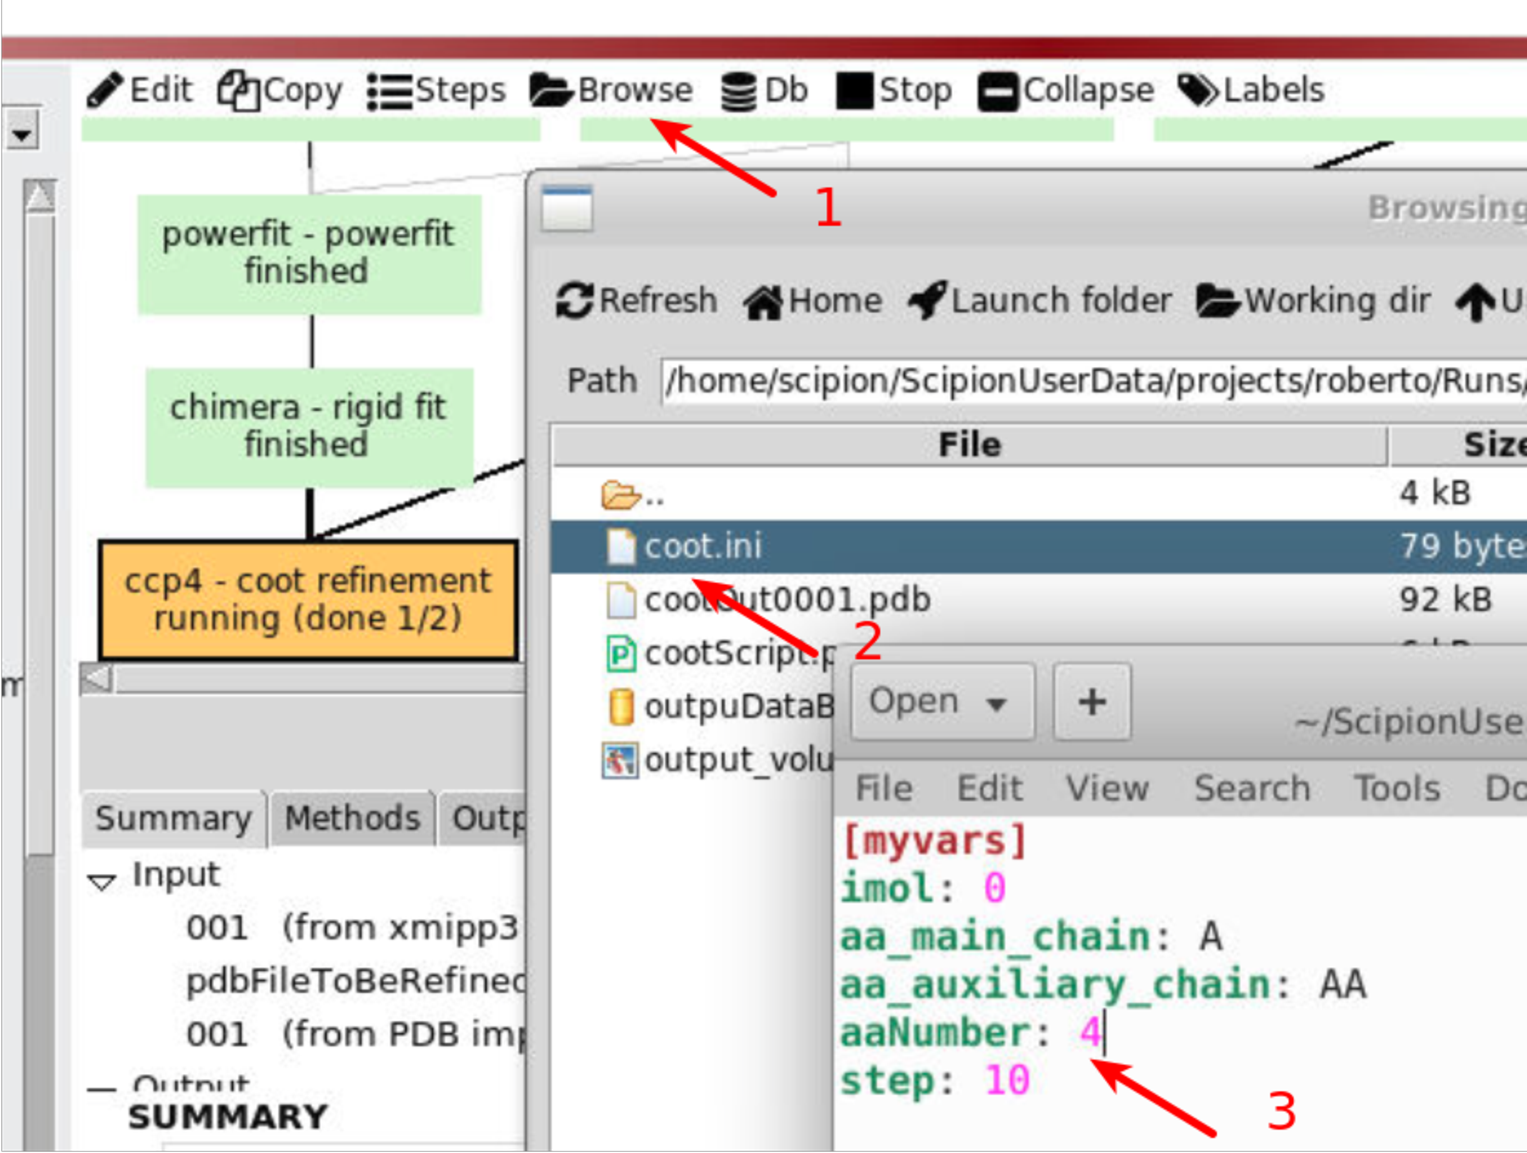
\includegraphics[width=0.80\textwidth]{Images/cootini}
  \caption{Edit coot.ini file.}
  \label{fig:cootini}
  \end{figure}
  
 %[**ROB coot need a careful presentation]
 %[**ROB preguntar a ERney por su metodo de filtracion]
 Finally, go back to \coot window and press ``U'' to initiate global variables and ``z'' to refine the next upstream 10 residues. Go through those residues, one by one, and accept refinement if you agree with it. If you disagree with the refinement of any residue, perform the interactive refinement, visualizing the residue side chain. Repeat the refinement process with ``z'' until the end of the molecule. Check that the orange bar of residue number 50 (\ffigure{fig:coot_density_fit_analysis}) goes missing at the end of this process.\\
 
 After this partially automatic and partially interactive processing, go to \ttt{Draw -> Go To Atom... -> Chain A -> A 2 VAL} (\ttt{VAL} is now the first residue of the \ttt{metHgb} $\alpha$ subunit) and start the detailed interactive refinement of the initial residues of chain A. To accomplish this interactive refinement of a small group of 5 to 10 residues, select the blue circle in the upper right side menu and click the initial and final residues of the small group of residues (\ffigure{fig:coot_go_to_atom} (B)(4)). The group of selected residues gets flexible enough to look manually for another spatial distribution. Following these instructions, try to solve the misfit that you can find in \ttt{TYR} 141 residue at the end of the molecule. Specifically, try to improve the result of the \ttt{Validate -> Density fit analysis}, as you can see from (A) to (B) in \ffigure{fig:coot_density_fit_analysis2}, moving \ttt{TYR} 141 ((A)(1)) to the nearest empty map density ((A)(2)). Accept the refinement parameters after the displacement of \ttt{TYR} ((B)(3)). Finally, check the \ttt{Density Fit Graph}.
 
  \begin{figure}[H]
  \centering 
  \captionsetup{width=.7\linewidth} 
  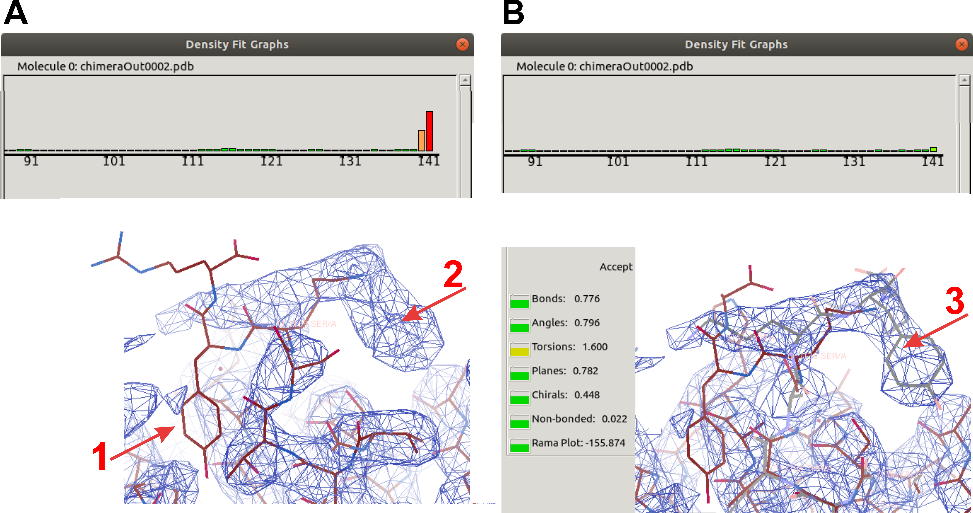
\includegraphics[width=0.85\textwidth]{Images/Fig28}
  \caption{\coot fit in the map density of residue \ttt{TYR} 141.}
  \label{fig:coot_density_fit_analysis2}
  \end{figure}
  
 Rotamer refinement is another refinement tool available in \coot. You can try to improve your current $model$ modifying rotamers reported as incorrect in \ttt{Validate -> Rotamer analysis}. Otherwise, the next refinement program in modeling workflow (\phenix \ttt{real space refine}) will perform rotamer refinement.\\
 
 At the end of this interactive refinement with \coot, the refined atomic structure has to be saved. You can save the atomic structure with its default name by pressing \keys{w}. If you prefer another name, for instance ``HBA\_HUMAN.pdb'', it can be saved in \coot main menu \ttt{Calculate -> Scripting -> Python} and the \ttt{Coot Python Scripting} window will be opened. Assuming that \ttt{0} is your \iii{model} number, write in Command:\\
 \ttt{scipion\_write (0, 'HBA\_HUMAN')}\keys{\return}
 
 In its interactive way, \scommand{ccp4 - coot refinement} protocol can be launched again whenever you want in \scipion, and the last atomic structure saved will be loaded in \coot graphics window. This functionality of \scipion allows to stop the interactive refinement and restart the process in the last refinement step, maintaining each one of the intermediate refined structures saved in order in \scipion tutorial folder \ttt{/Runs/000XXX\_CootRefine/extra}. In this way, go again to intermediate refined structures is also possible. Finally, when you reach the final refined structure save it, and you may press \keys{e} to fully stop protocol \coot.\\
 
 A similar refinement process to that followed in \coot for \ttt{metHgb} $\alpha$ subunit chain \ttt{A}, has to be carried out for chain \ttt{HEME} and for respective chains of \ttt{metHgb} $\beta$ subunit.\\
 
 
 \subsection*{\phenix Real Space Refine}
 
 In order to compare the previous \coot interactive refinement with an automatic refinement, we are going to use the
 \scommand{phenix - real space refine} protocol in parallel. This protocol implements in \scipion the \iii{phenix.real\_space\_refine} program developed to address cryo-EM structure-refinement requirements. Following a workflow similar to the \phenix reciprocal-space refinement program \iii{phenix.refine}, basically devoted to crystallography, \iii{phenix.real\_space\_refine} program, mainly used in cryo-EM, is able to refine in real space atomic models against maps, which are the experimental data.\\
 
 Start working by opening \scommand{phenix - real space refine} protocol (\ffigure{fig:phenix_real_space_refine_protocol} (1)), load as input volume the extracted unit cell saved in \coot (2), write the volume resolution (3), load the atomic structure ($model$ \ttt{chimeraOut0002.pdb}, (4)) and select the output format of the refined atomic structure that will be generated (5). After executing the protocol (6), results can be checked (7). 
 
 \begin{figure}[H]
  \centering 
  \captionsetup{width=.7\linewidth} 
  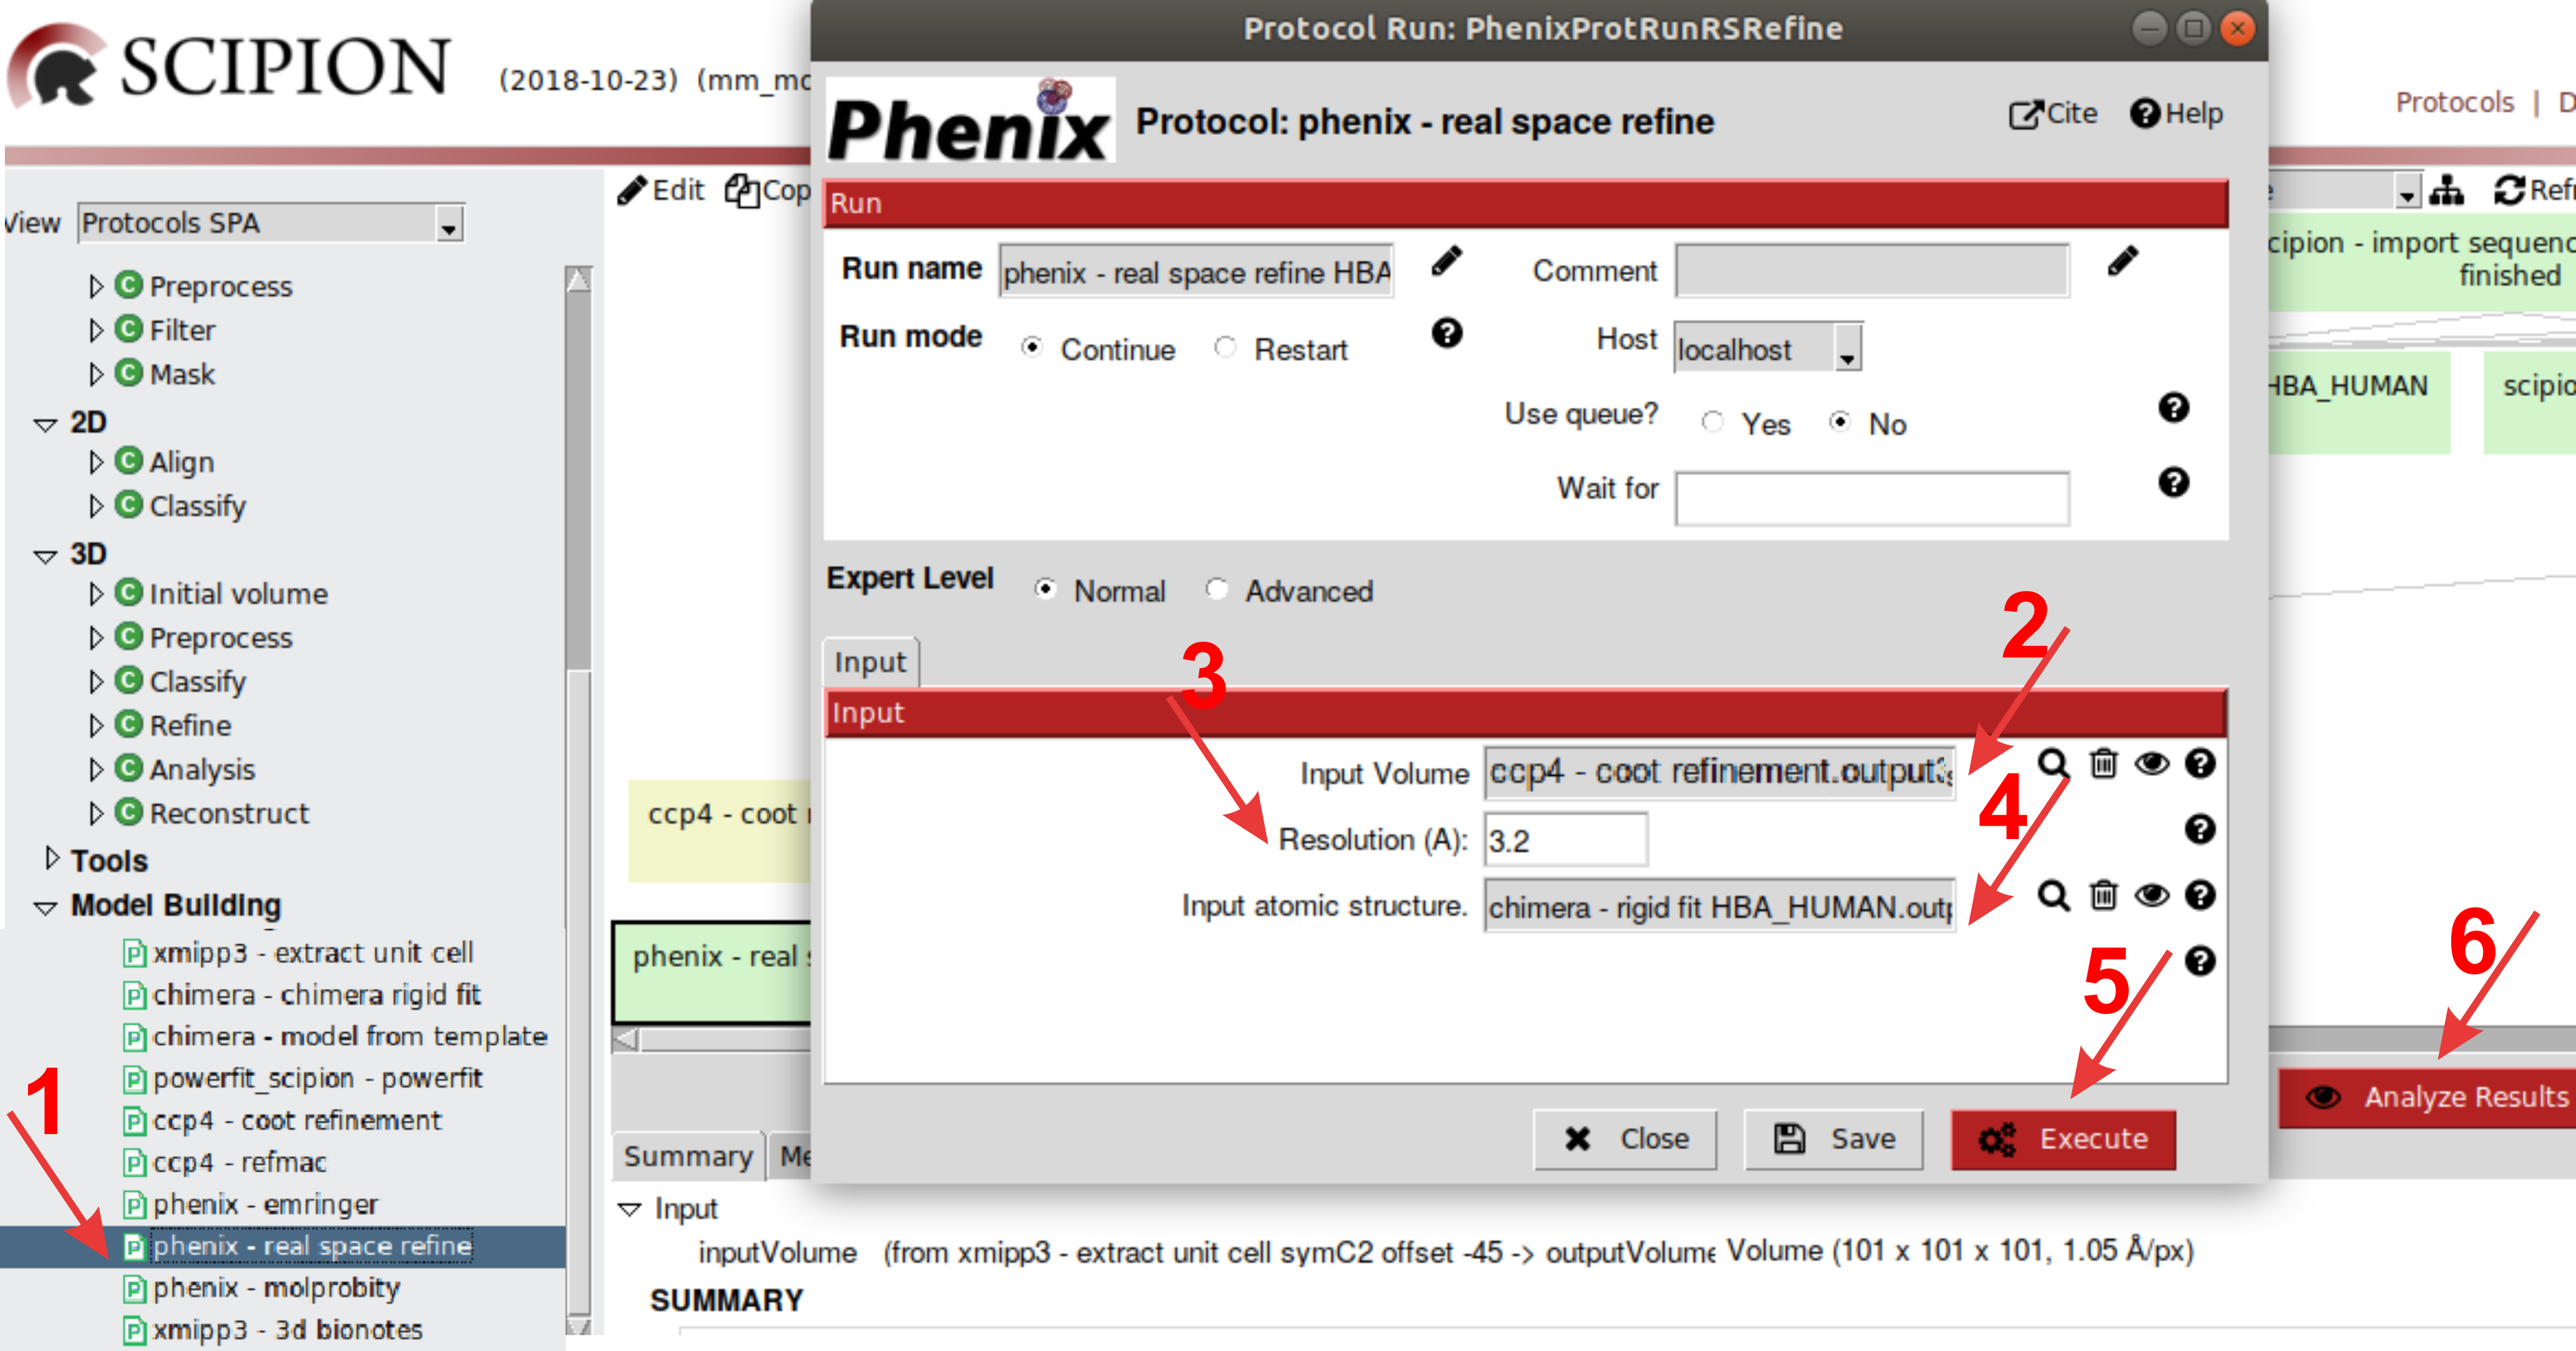
\includegraphics[width=0.85\textwidth]{Images/Fig29}
  \caption{Completing \phenix Real Space Refine protocol.}
  \label{fig:phenix_real_space_refine_protocol}
  \end{figure}
 
 The first tab of results shows the initial $model$ atomic structure as well as the refined one, both fitted to the normalized extract unit cell volume saved in \coot (\ffigure{fig:phenix_real_space_refine_chimera}). 
 
 \begin{figure}[H]
  \centering 
  \captionsetup{width=.7\linewidth} 
  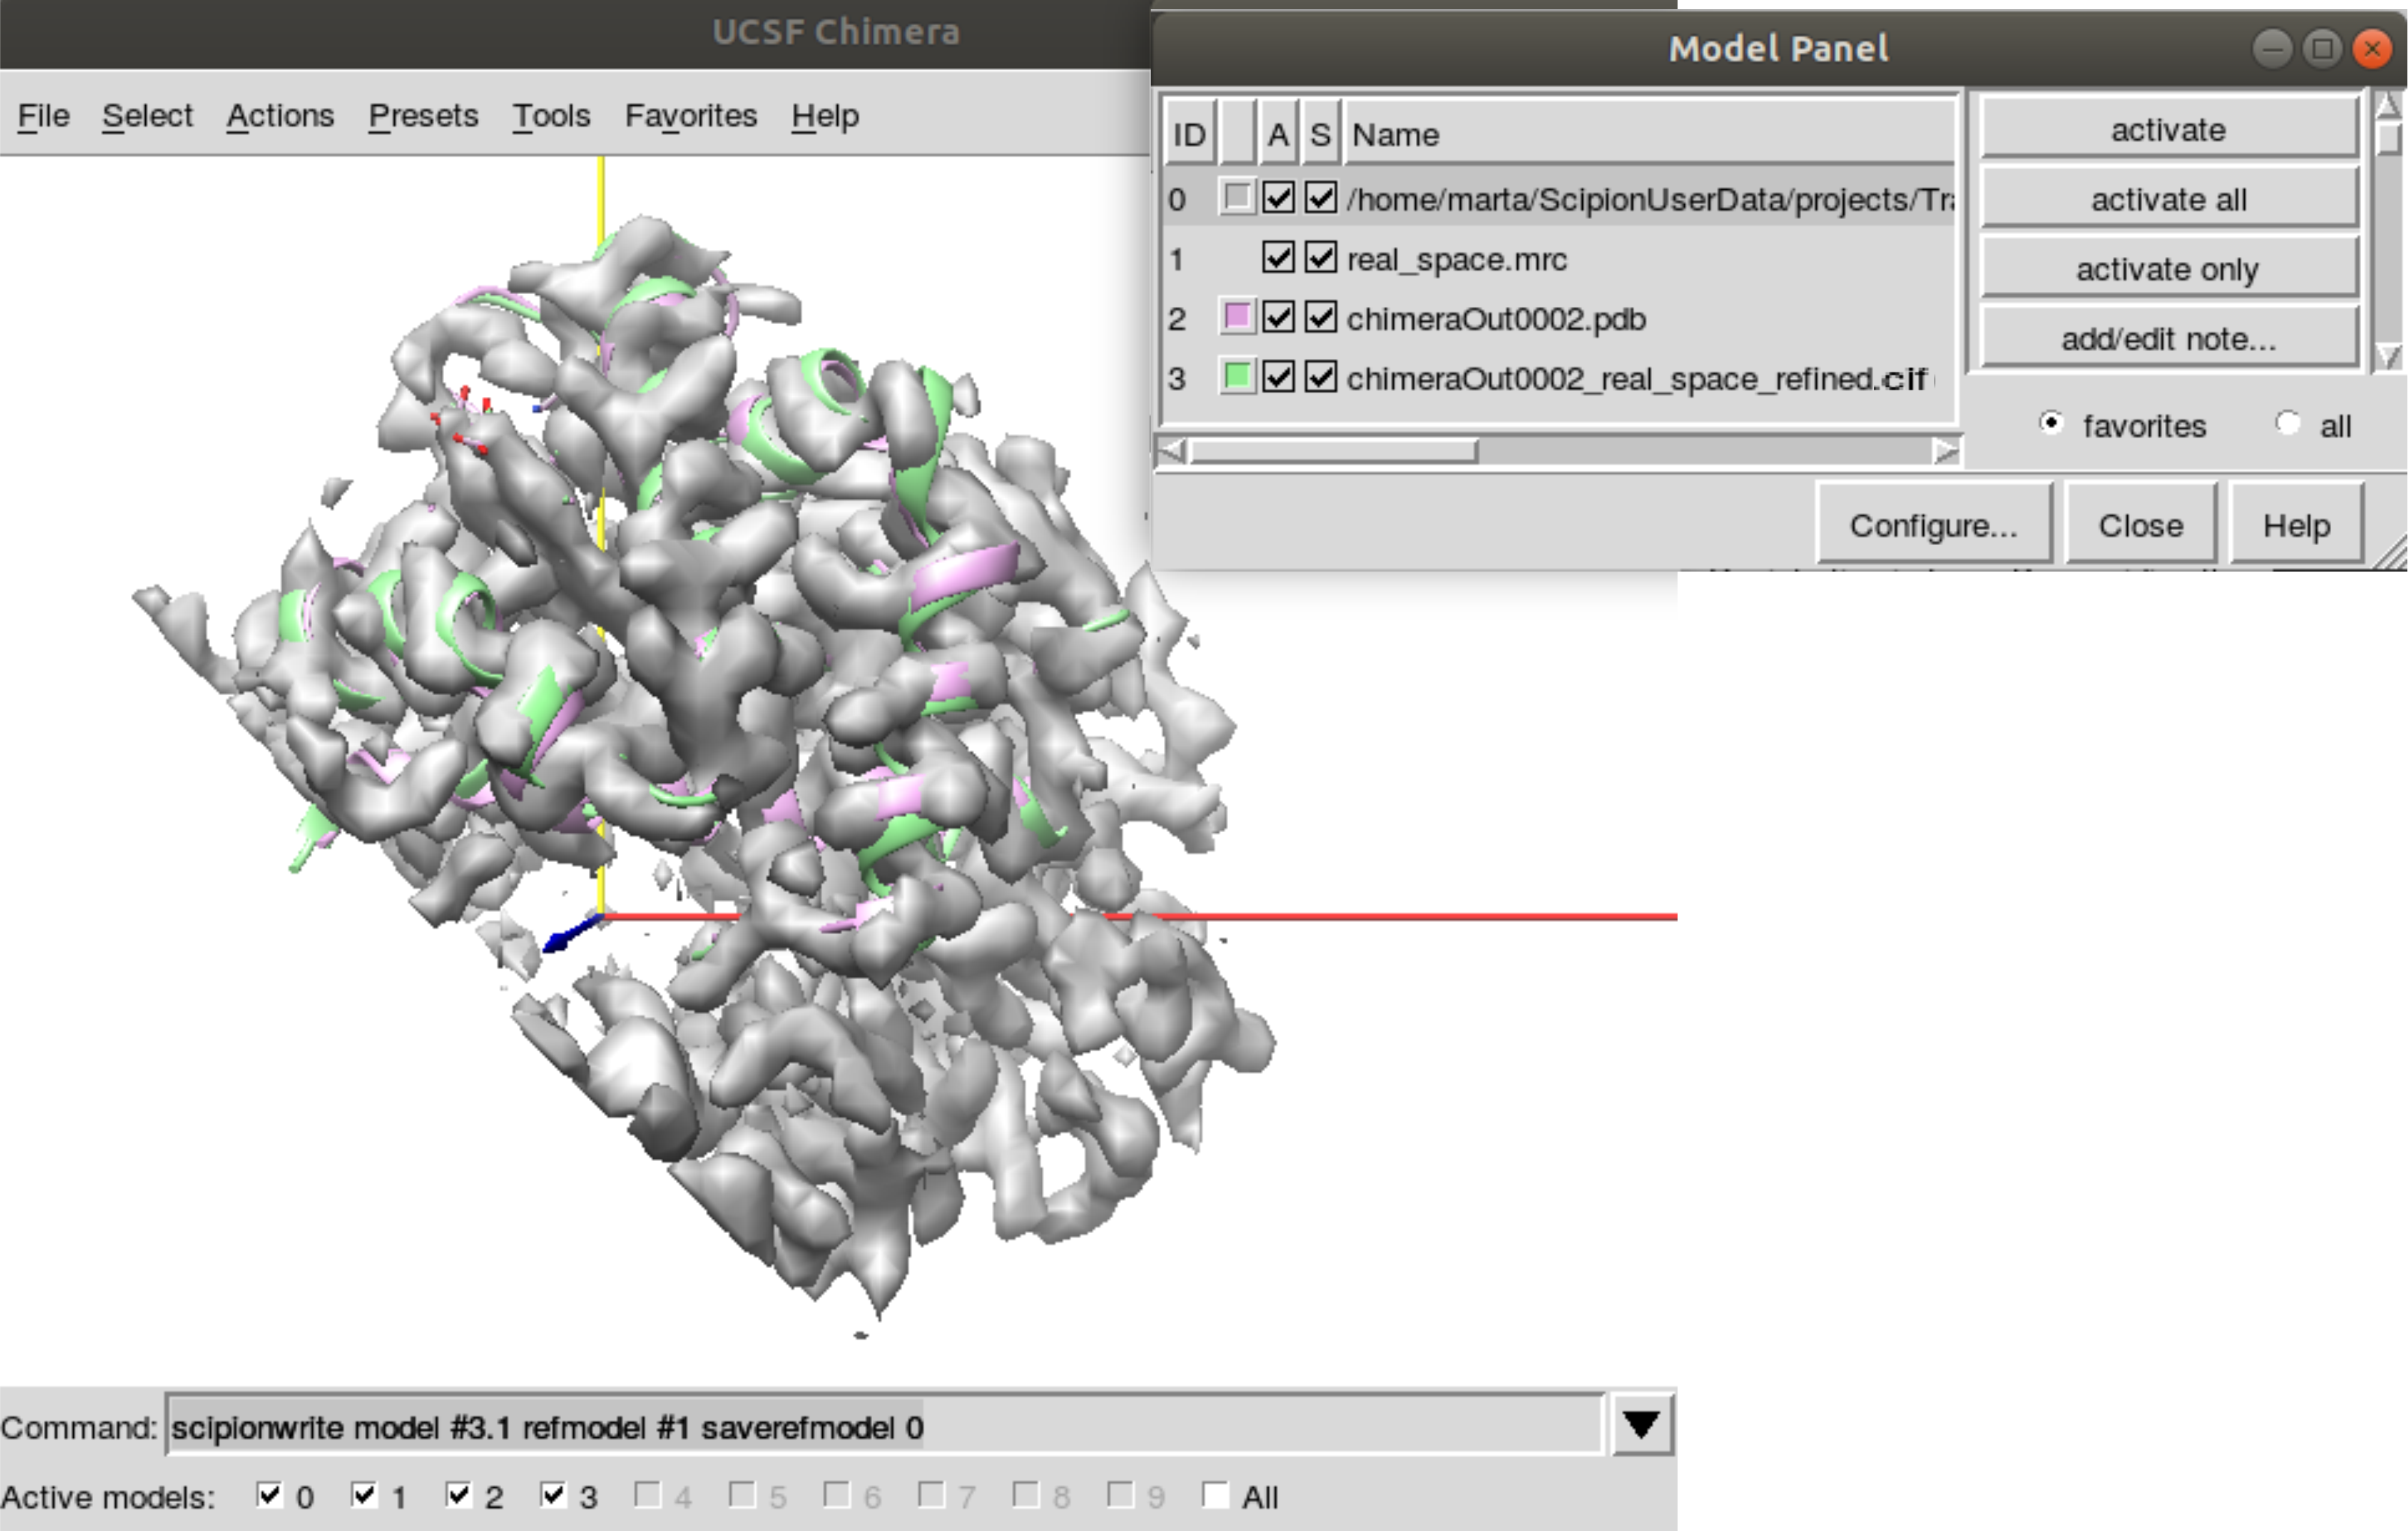
\includegraphics[width=0.85\textwidth]{Images/Fig30}
  \caption{\chimera visualization of refined $model$ of \ttt{metHgb} $\alpha$ subunit by \phenix Real Space Refine protocol.}
  \label{fig:phenix_real_space_refine_chimera}
  \end{figure}
  
  The rest of tabs detail different statistics useful to compare the quality of distinct $models$ such as $MolProbity$ statistics and \ttt{Real-space} correlations. $MolProbity$ results will be discussed in the next section of validation and comparison. Regarding \ttt{Real-space} correlations, different $mdels$ can be compared by using the global number of \ccmask, that indicates the correlation $model$-to-map calculated considering the map region masked around the $model$. You can check also individual correlation values for each residue.  Remark that residues with lower correlation values might be susceptible to improve by additional refinement in \coot. Have a look to those correlation values and answer the following questions: (Answers in appendix \ref{app:solutions}; \textbf{Question \ref{refinementFlexibleFitting}\_1}) \\
  
  \begin{minipage}{\linewidth}
  \begin{framed}
  \begin{itemize}
  \item What is the \ccmask value?
  \item Which one is the residue that shows the lower correlation value? Why?
  \item What is that correlation value?
  \item Which one is the second residue that shows the lower correlation value? Why?
  \item What is that correlation value?
  \item What is the correlation value of \ttt{HEME} group?
  \end{itemize}
  \end{framed}
  \end{minipage}\\
  
  The conclusion of this part of refinement in real space is that \coot and \phenix \ttt{real space refine} might perform complementary tasks. The usage of both protocols may improve the result, especially when partial processing or big arrangements of molecules are involved. Now, to take advance of $model$ improvements performed with \coot, run \phenix \ttt{real space refine} after \coot. When you finish, check again the above values of correlation. Have they changed? (Answer in appendix \ref{app:solutions}; \textbf{Question \ref{refinementFlexibleFitting}\_2})
  
  Before finishing our refinement workflow with \refmac, we can ask ourselves how can we improve correlations in real space by modifying the advance parameters in the protocol form. Will the correlation values change if we set to ``yes'' optimization parameters previously set to ``no'' and increase the number of macro cycles from 5 to 30? Take into account that this process take much more time (around 6 times more) than the previous one. (Answer in appendix \ref{app:solutions}; \textbf{Question \ref{refinementFlexibleFitting}\_3})\\
  
  \subsection*{\ccp4  \refmac}
  
  As in the case of \coot, \refmac (from maximum-likelihood Refinement of Macromolecules) was initially developed to optimize models obtained by X-ray crystallography methods, but unlike \coot, automatically and in reciprocal space. The $models$ refined in the real space with \coot and \phenix \ttt{real space refine}, successively, will be used as input to perform a second refinement step in the Fourier space with \refmac protocol \scommand{ccp4 - refmac}. Firstly, open the \refmac protocol form (\ffigure{fig:refmac_protocol} (1)), load the volume generated by \coot (2), the atomic structure obtained with \phenix \ttt{real space refine} (3), and the volume resolution as maximum resolution (4). Execute the protocol (5) and when it finish, analyze the results (6).
  
  \begin{figure}[H]
  \centering 
  \captionsetup{width=.7\linewidth} 
  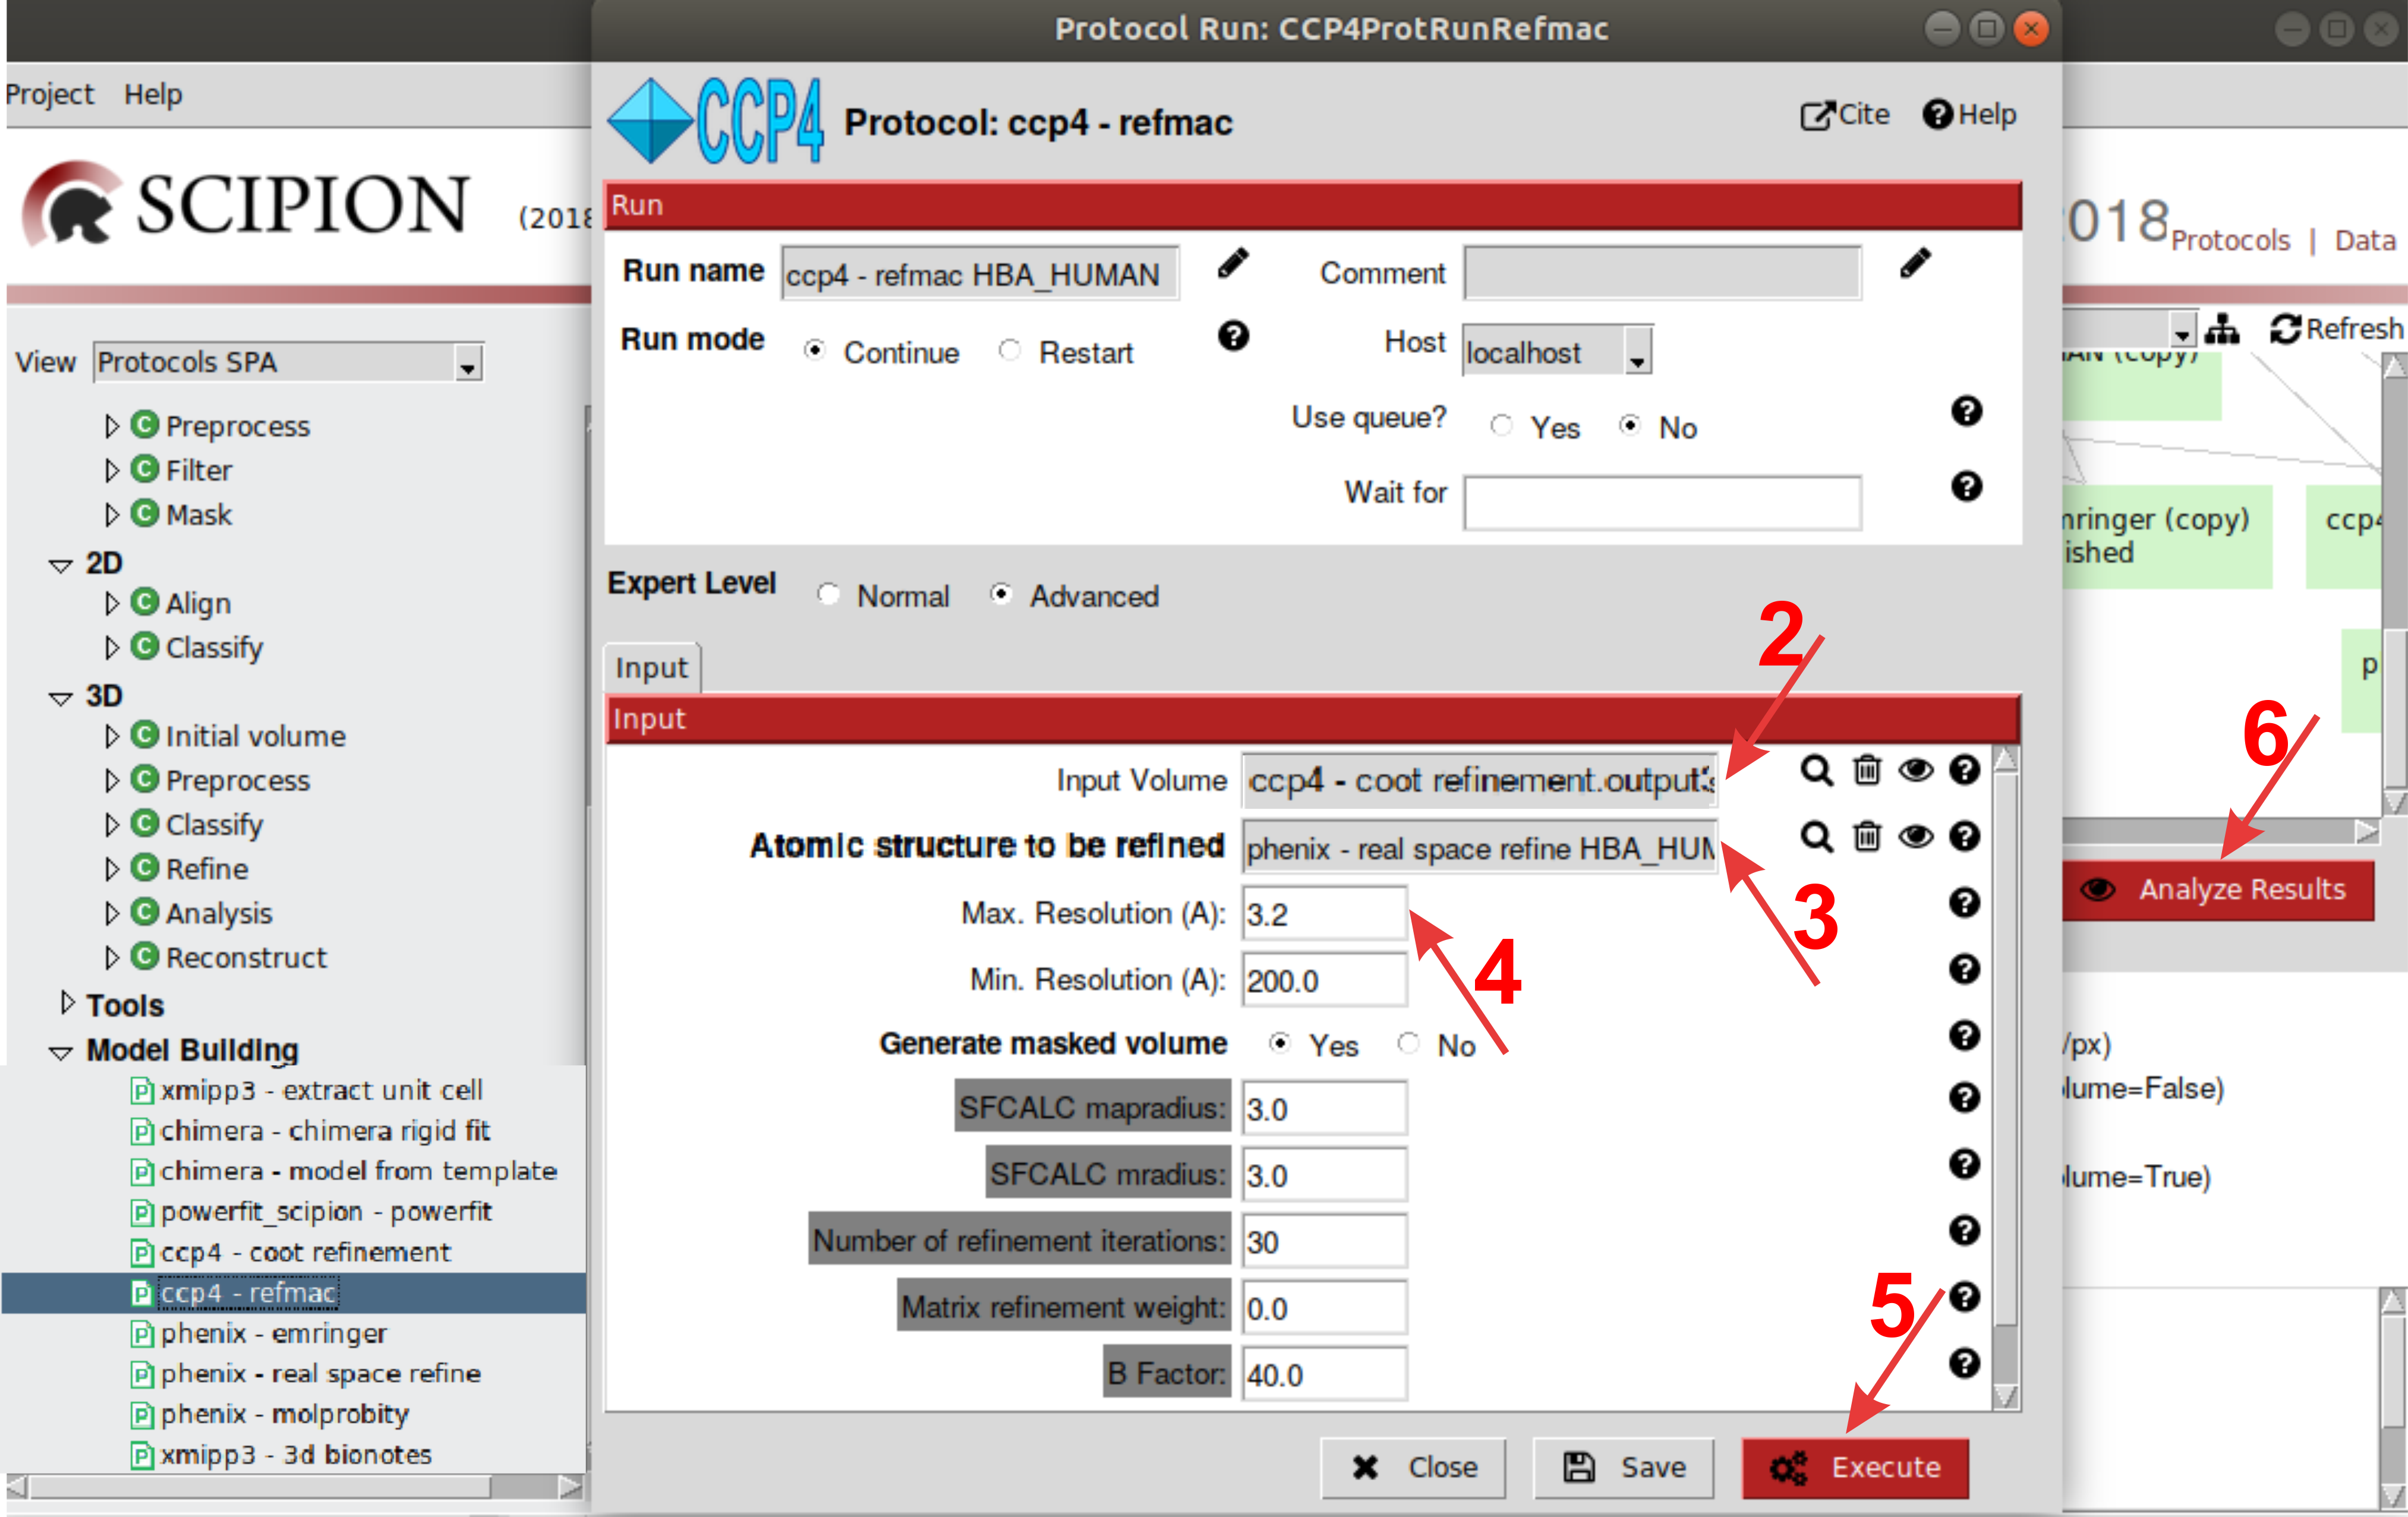
\includegraphics[width=0.85\textwidth]{Images/Fig31}
  \caption{Filling in \refmac protocol.}
  \label{fig:refmac_protocol}
  \end{figure}
  %[**ROB mask display in chimera is not centered **]
  Clicking the first item in the display menu of results (\ffigure{fig:refmac_protocol} (1)), \chimera graphics window will be opened showing the input volume, the initial $model$ (\ttt{HBA\_HUMAN} obtained with \phenix \ttt{real space refine}), and the final \refmac refined $model$ (\ffigure{fig:refmac_chimera}). By clicking the third item in the display menu of results (\ffigure{fig:refmac_protocol} (2)), a summary of \refmac results are shown. Check if values of \ttt{R factor} and \ttt{Rms BondLength} have improved with this refinement process. Why the improvement seems to be very small? (Answers in appendix \ref{app:solutions}; \textbf{Question \ref{refinementFlexibleFitting}\_4})\\
  
  Would you have seen a higher improvement running \refmac immediately after \coot, thus ignoring $model$ improvements generated by \phenix \ttt{real space refine}? (Answers in appendix \ref{app:solutions}; \textbf{Question \ref{refinementFlexibleFitting}\_5})\\
  
  Regarding the using of mask: Compare \refmac results (after \coot and \phenix \ttt{real space refine}) with those obtained selecting the option \ttt{No} in the protocol form parameter \ttt{Generate masked volume}. Use two different volumes, the one generated by \coot protocol, and the one generated by the \ttt{extract unit cell} protocol. Are there any differences? Why? (Answers in appendix \ref{app:solutions}; \textbf{Question \ref{refinementFlexibleFitting}\_6})\\
  
  \begin{figure}[H]
  \centering 
  \captionsetup{width=.7\linewidth} 
  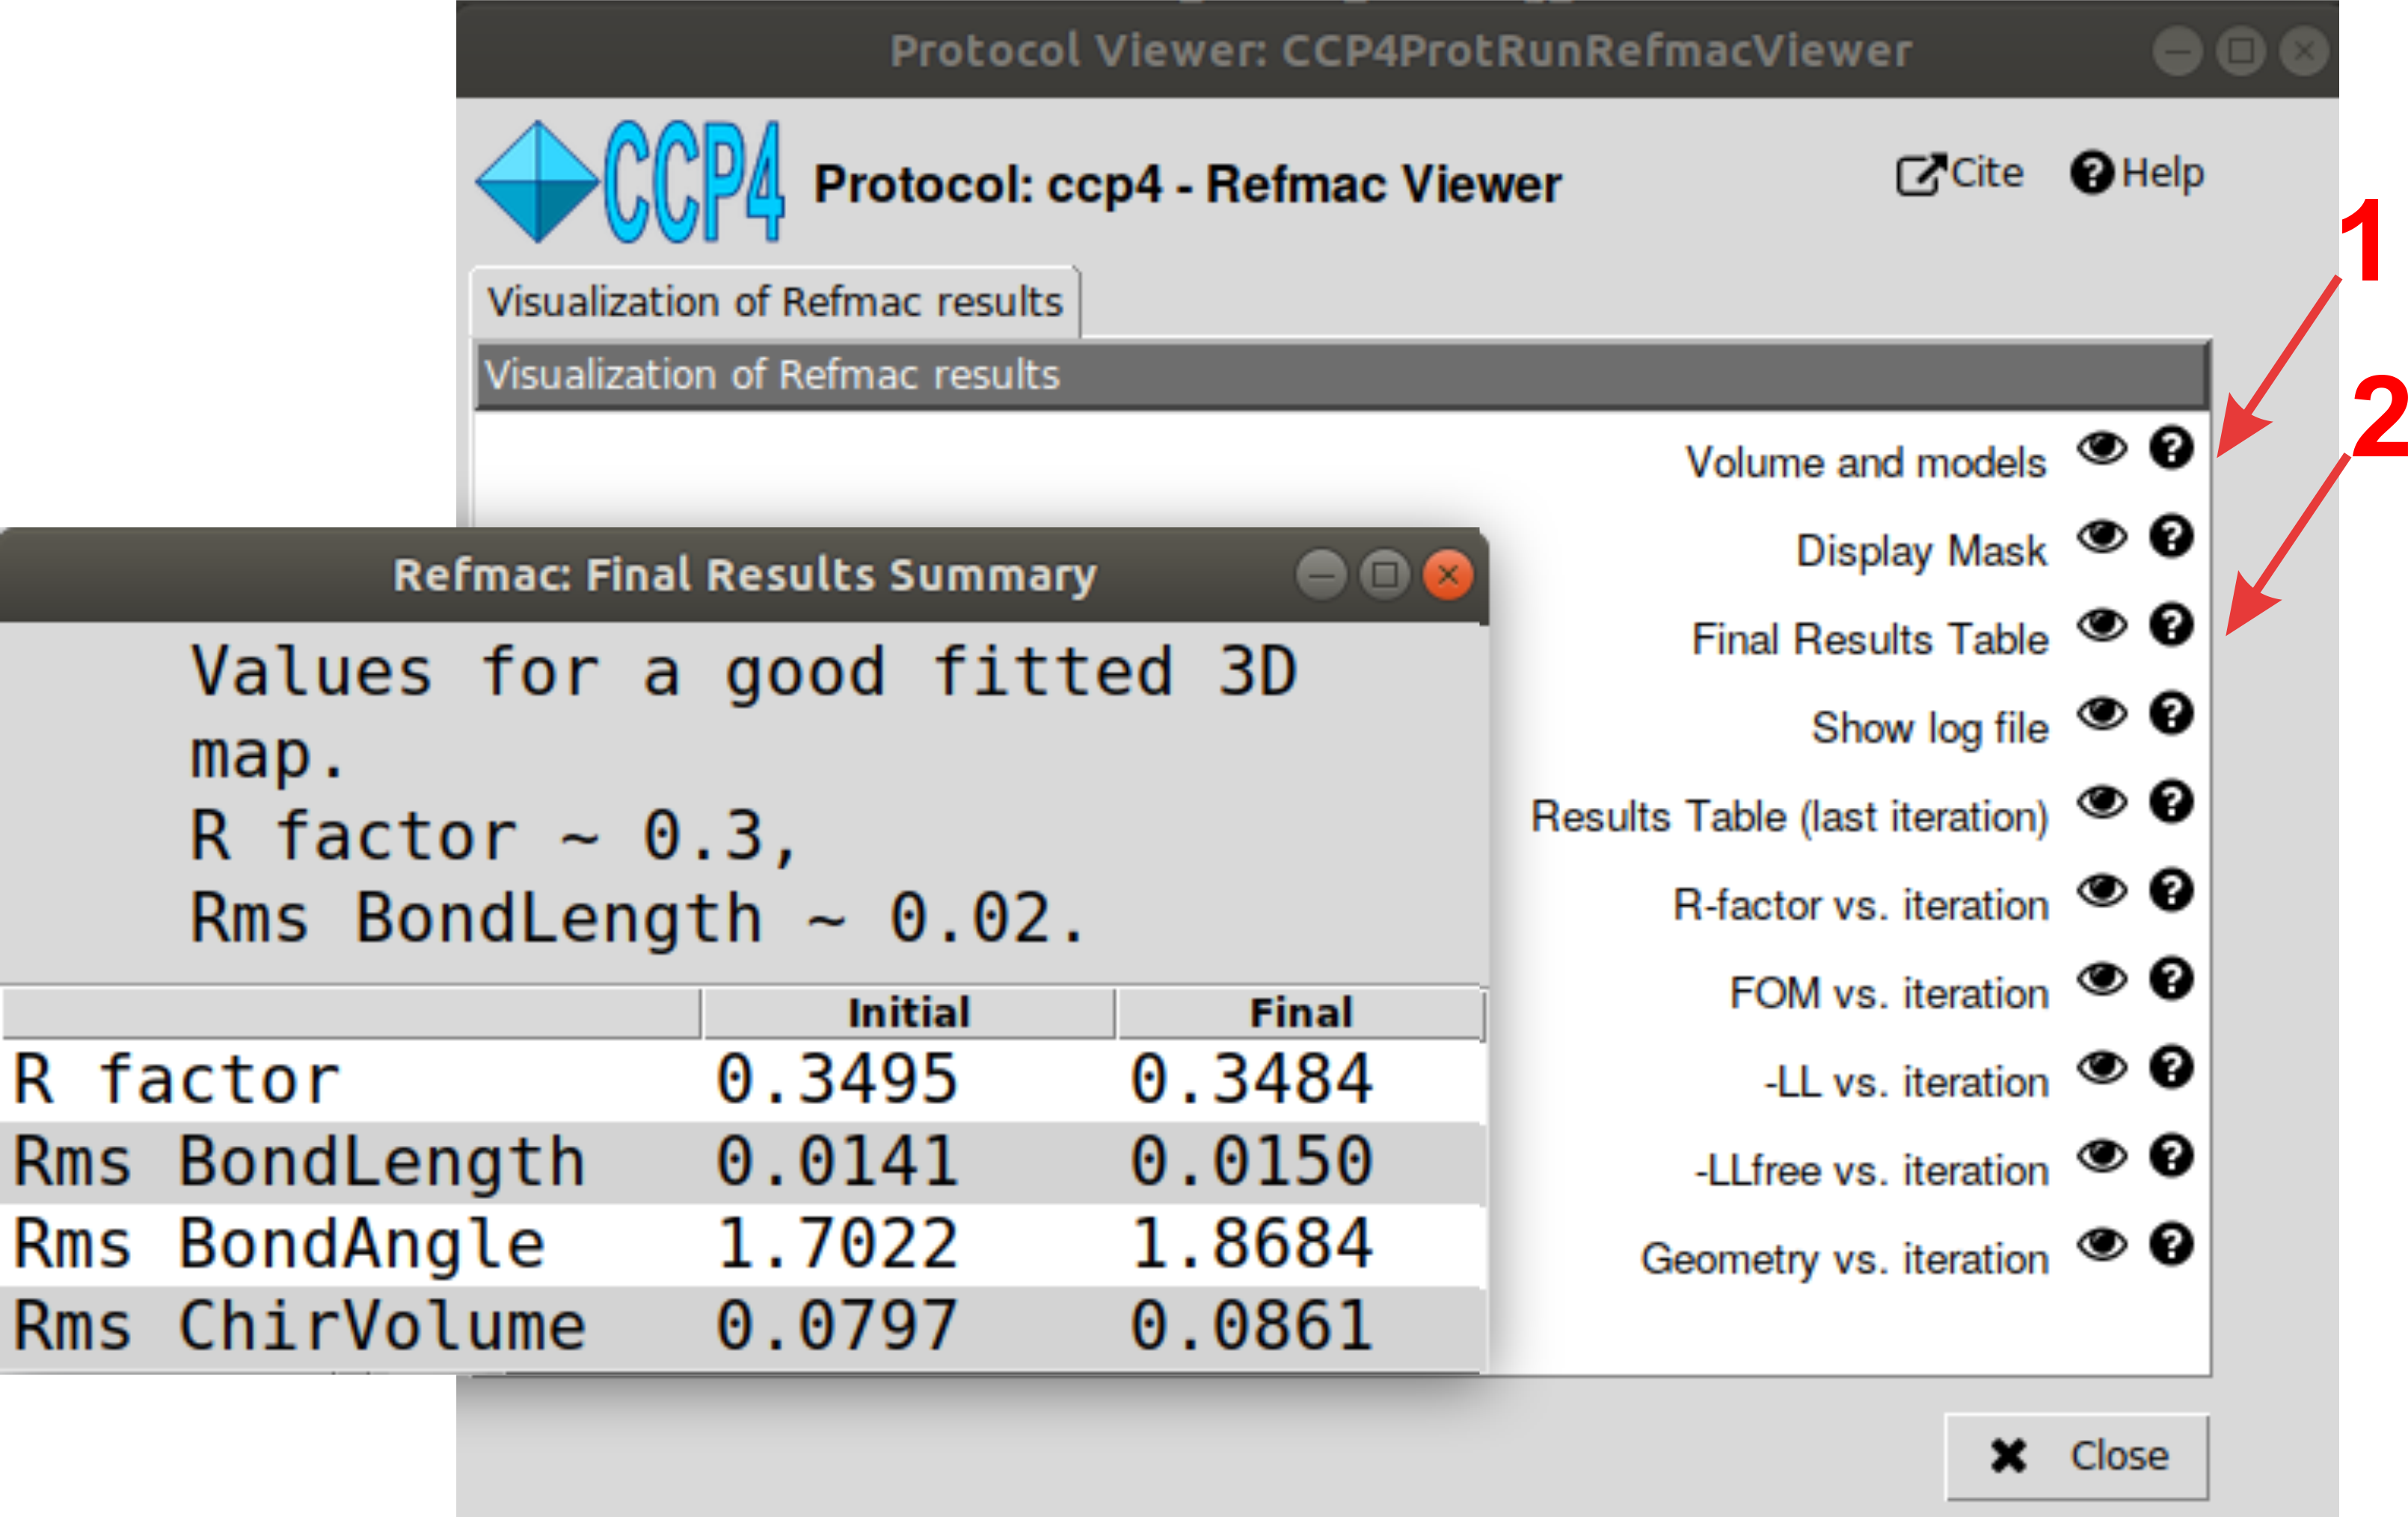
\includegraphics[width=0.85\textwidth]{Images/Fig32}
  \caption{Display menu of \refmac results.}
  \label{fig:refmac_display_results}
  \end{figure}
  
  \begin{figure}[H]
  \centering 
  \captionsetup{width=.7\linewidth} 
  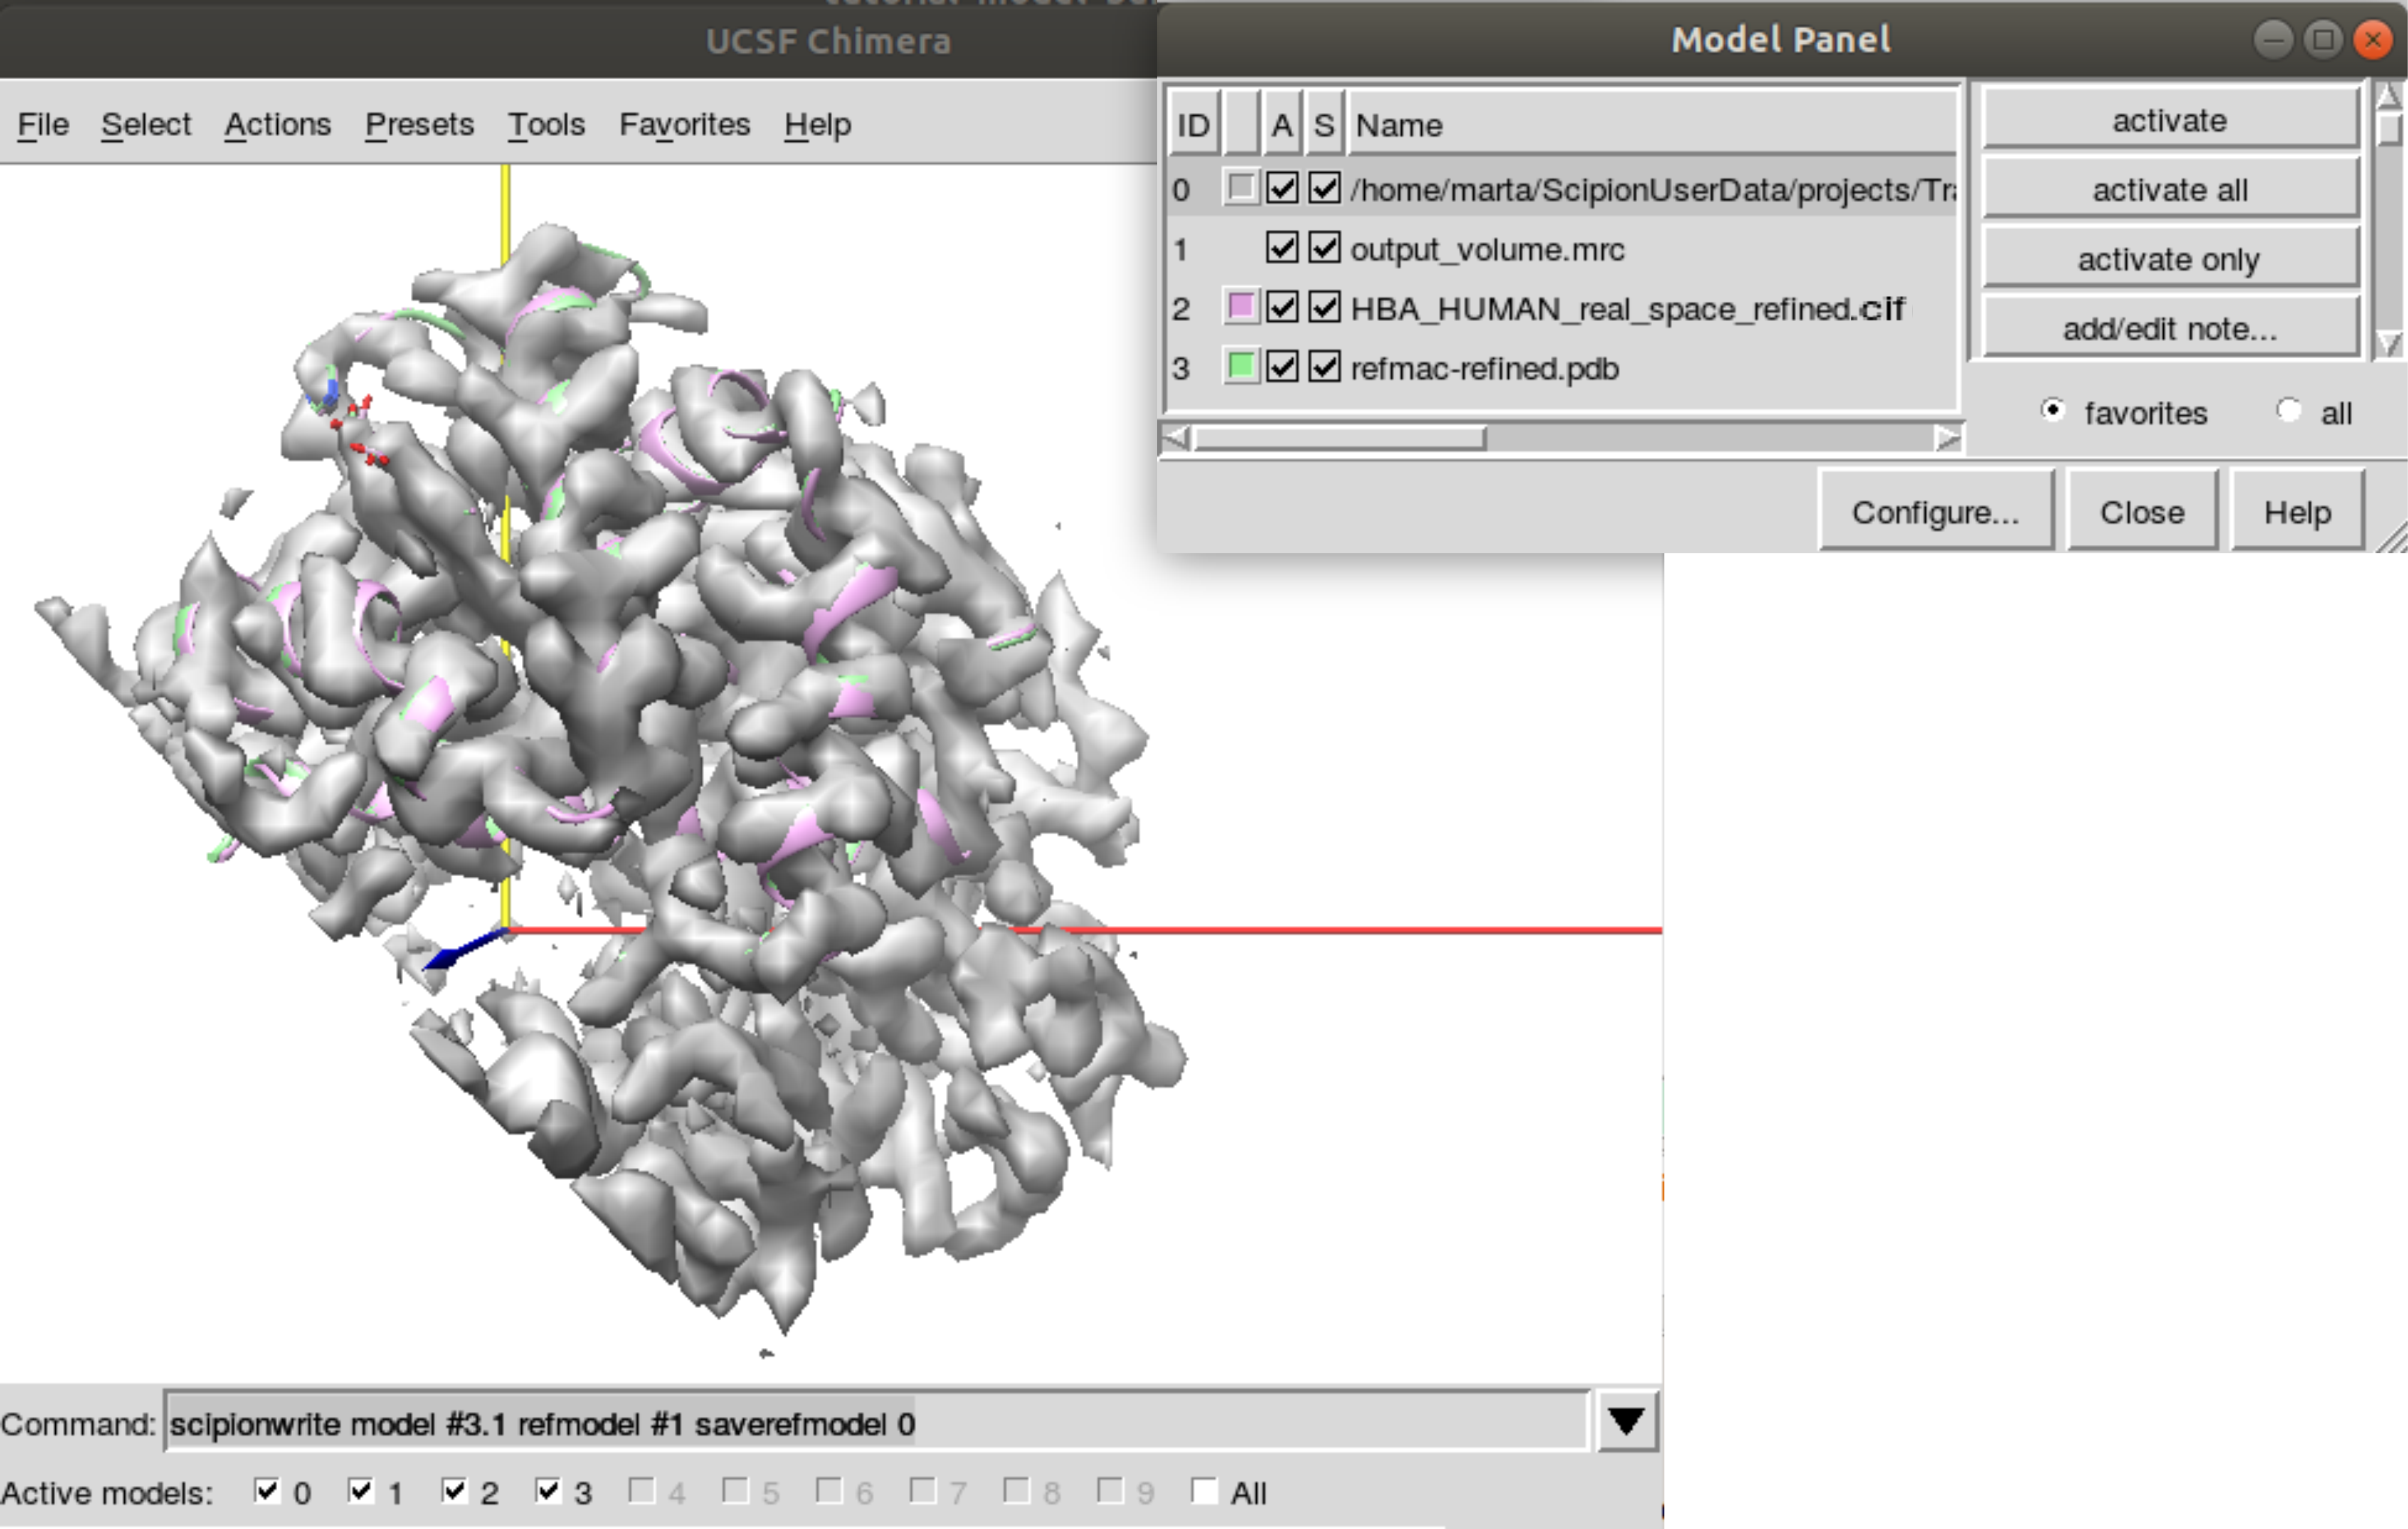
\includegraphics[width=0.85\textwidth]{Images/Fig33}
  \caption{\chimera visualization of refined $model$ of \ttt{metHgb} $\alpha$ subunit by \refmac.}
  \label{fig:refmac_chimera}
  \end{figure}
  
  Have a look to the rest of items in the display window of results. 
  

\section{Structure validation and comparison}

 At the end of the refinement process of \ttt{metHgb} $\alpha$ subunit (a similar one would be required for $\beta$ subunit), we need to assess the geometry of our $model$ regarding the starting 
volume to detect $model$ controversial elements or $model$ parameters that disagree with the map. Although each refinement program has their own tools to assess the progress of refinement ($Coot$ \ttt{Validate} menu; $Phenix$ \ttt{real space refine} real space correlations; $Refmac$ \ttt{R factor} and \ttt{Rms BondLength}), in this tutorial section, two assessment tools will be described to obtain comparative validation values after using any protocol in the workflow:  Protocols $EMRinger$ (\scommand{phenix - emringer}, Appendix \ref{app:emRingerProtocol}, \citep{barad2015}) and $MolProbity$ (\scommand{phenix - molprobity}, Appendix \ref{app:molprobityProtocol}, \citep{davis2004}). As in $Phenix$, correlation values in real space will be computed if a volume is provided with $MolProbity$ protocol. Additionally, we are going to introduce the protocol \scommand{phenix - superpose pdbs} (Appendix \ref{app:superposePdbsProtocol}, \citep{zwartUrl}) useful to compare visually the geometry of two atomic structures.\\

\begin{itemize}

 \item $EMRinger$:\\
 
 Specifically designed for cryo-EM data, $EMRinger$ tool assesses the appropriate fitting of a model to a map, validating high-resolution features such as side chain arrangements. The placement of side chains regarding the molecule skeleton depends on the $\chi_{1}$ dihedral angle, which is determined by atomic positions of \ttt{N}, \ttt{C$\alpha$}, \ttt{C$\beta$} and \ttt{C$\gamma$}. The $model$ backbone well fitted should be enriched in rotameric $\chi_{1}$ dihedral angles of 60º, 180º and 300º (-60º). The lower deviations regarding these values, the better $model$, and the higher EMRinger value.  
 
 We can start assessing with $EMRinger$ the \ttt{metHgb} $\alpha$ subunit $models$ that we have generated along the modeling workflow. In each case, open the \scommand{phenix - emringer} protocol ((\ffigure{fig:emringer_protocol} (1)), load the extracted unit cell volume (initial or saved with $Coot$) (2) and the atomic structure that you'd like to validate in relation to the volume (3), execute the program (4) and analyze results (5). A menu to check results in detail will be opened (bar \ttt{EMRinger results}). \iii{Phenix EMRinger} plots with density thresholds, with rolling window for each chain, as well as dihedral angles for each residue are shown here. The most relevant results, especially the EMRinger score, will also be written in the protocol \ttt{SUMMARY} (6). 
 
  \begin{figure}[H]
  \centering 
  \captionsetup{width=.7\linewidth} 
  \includegraphics[width=0.85\textwidth]{Images/Fig34}
  \caption{Completing $EMRinger$ protocol form.}
  \label{fig:emringer_protocol}
  \end{figure}
 
 Run $EMRinger$ protocol and determine the respective score after running \iii{PowerFit item2}, $Chimera$ \ttt{rigid fit} ($model$ 2), $Coot$ refinement, $Phenix$ \ttt{real space refine} after $Coot$ (default conditions and last modification of form parameters), and $Refmac$ refinement with MASK before and after $Phenix$ \ttt{real space refine}. Considering $EMRinger$ \ttt{score}, does our \ttt{metHgb} $\alpha$ subunit $models$ seem to be OK? (Answers in appendix \ref{app:solutions}; \textbf{Question 8}). Try the same validation with $\beta$ subunit $models$. \\
 
 \item $MolProbity$:\\
 
 The atomic structure validation web service $MolProbity$, with better reference data has been implemented in the open-source CCTBX portion of $Phenix$ \citep{williams2018}. This widely used tool assesses $model$ geometry and quality at both global and local levels. Originally designed to evaluate structures coming from X-Ray diffraction and NMR, it does not take into account the quality of the fitting with a 3D density map.  The implementation in $Phenix$, nevertheless, includes the possibility of adding a volume and assessing the correlation in the real space.\\
 
 The assessment process that we have carried out with $EMRinger$ can also be done with $MolProbity$ in \scipion. We are going to validate the geometry of \ttt{metHgb} $\alpha$ subunit $models$ that we have generated along the modeling workflow. In each case, open the \scommand{phenix - molprobity} protocol (\ffigure{fig:molprobity_protocol} (1)), load the extracted unit cell volume (initial or generated by $Coot$) (2) wit its resolution (3) if you want to have real space correlation between map and $model$, load the $model$ atomic structure (4) and execute the protocol (5). In \ttt{Analyze results} (6) the same menu bars available in results section of $Phenix$ \ttt{real space refine} protocol are shown here. $MolProbity$ results bar include validation statistics. Protocol \ttt{SUMMARY} emphasizes the most relevant ones.\\
 
 \begin{figure}[H]
  \centering 
  \captionsetup{width=.7\linewidth} 
  \includegraphics[width=0.85\textwidth]{Images/Fig35}
  \caption{Completing $MolProbity$ protocol form.}
  \label{fig:molprobity_protocol}
  \end{figure}
  
  Run $MolProbity$ protocol to obtain its statistics values after running \iii{PowerFit item2}, $Chimera$ \ttt{rigid fit} ($model$ 2), $Coot$ refinement, $Phenix$ \ttt{real space refine} (default conditions and last modification of form parameters) after $Coot$, and $Refmac$ refinement with MASK before and after $Phenix$ \ttt{real space refine}. In order to compare validation results of $models$ obtained along the modeling workflow, fill in the next table (\ttable{table:empty}) including, in addition to $MolProbity$ statistics, $EMRinger$ scores and \ccmask values obtained before. (Answers in appendix \ref{app:solutions}; \textbf{Question 9}). The same table (\ttable{table:empty}) can be completed for \ttt{metHgb} $\beta$ subunit (Appendix \ref{app:solutions}; \textbf{Question 10})\\
  
  \begin{sidewaystable}
   \caption{Validation statistics of human \ttt{metHgb} $\alpha$ subunit $model$. \ttt{RSRAC} stands for \ttt{Real Space Refine} after $Coot$. \ttt{Rama} stands for \ttt{Ramachandran}.}
   \centering\footnotesize
   \begin{tabular}{l c c c c c c c c}
   \hline\hline
   Statistic &  \thead{$Powerfit$\\ $item$ \#2} & \thead{$Chimera$\\ $model$ \#2} & $Coot$ & \thead{$Phenix$\\ \ttt{RSRAC}\\(default)} & \thead{$Phenix$\\ \ttt{RSRAC}\\(modified)} & \thead{$Refmac$\\ after $Coot$} & \thead{$Refmac$\\ after \ttt{RSRAC}\\(modified)} & \ttt{5NI1}\\ [0.5ex]
   \hline
   \ccmask \\
   $EMRinger$ \ttt{score} \\
   \ttt{RMS} (Bonds) \\
   \ttt{RMS} (Angles) \\
   \ttt{Rama favored} (\%) \\
   \ttt{Rama allowed} (\%) \\
   \ttt{Rama outliers} (\%) \\
   \ttt{Rotamer outliers} (\%) \\
   \ttt{Clashscore} \\
   \ttt{Overall score} \\
   \ttt{C$\beta$ deviations} \\
   \ttt{RMSD} \\[1ex] 
   \hline
   \end{tabular}
   \label{table:empty}
   \end{sidewaystable}
 
 
 Results compiled in this table indicate that statistics are uncorrelated. From the point of view of correlation in real space, the best $model$ was obtained from $Phenix$ \ttt{real space refine} (last modification of form parameters) after $Coot$. Considering $EMRinger$ \ttt{score}, the best $model$ derives from the whole workflow $Coot$ \ttt{->} $Phenix$ \ttt{real space refine} (default conditions). With $MolProbity$ \ttt{Overall score} as validation rule, the last step in the workflow could be suppressed because the best value was obtained after $Coot$ \ttt{->} $Phenix$ \ttt{real space refine} (last modification of parameters). We'd like to select the best $model$ and continue refining it in order to improve it as much as possible. Assuming that no one $model$ is perfect, how can we select the best one?\\ 


 \item $Model$ Comparison:\\
 
 The question posed in the previous item does not have an easy answer in the real world, in which we do not know the final atomic structure. In this tutorial, nevertheless, we know it and we can wonder how far we are of the atomic structure already published for this cryo-EM map. The question can be answered by comparing a) validation statistics that we have obtained for our $models$ with the statistics computed for the available $\alpha$ subunit in \ttt{PDB} structure \ttt{5NI1}, and b) the atomic structures themselves by overlapping.\\ 
    
  \begin{itemize}
  \item Comparison of validation statistics: \\
  
  Validation statistics of \ttt{metHgb} $\alpha$ subunit of \ttt{PDB} structure \ttt{5NI1} should be obtained as first step to compare them with our $models$ validation statistics. With this aim we are going to follow the next workflow:\\
  \begin{itemize}
    \item Protocol \scommand{import atomic structure}:\\
    Download from \ttt{PDB} structure \ttt{5NI1}\\
    
    \item Protocol \scommand{chimera operate} (Appendix \ref{app:chimeraOperate}):\\
    Similar to $Chimera$ \ttt{rigid fit}, $Chimera$ \ttt{operate} protocol allows to perform operations with atomic structures. We are going to use this protocol to save independently in \scipion the \ttt{metHgb} $\alpha$ subunit. Open the protocol  (\ffigure{fig:chimera_operate_protocol} (1)), complete the parameter \ttt{PDBx/mmCIF} including the atomic structure \ttt{5NI1} previously imported (2), and execute the protocol (3).      
    
    \begin{figure}[H]
    \centering 
    \captionsetup{width=.7\linewidth} 
    \includegraphics[width=0.90\textwidth]{Images/Fig36}
    \caption{Filling in $Chimera$ \ttt{operate} protocol form.}
    \label{fig:chimera_operate_protocol}
    \end{figure}
    
    The $Chimera$ graphics window will be opened with the structure \ttt{5NI1} as model number \#1. To save independently the structure of human \ttt{metHgb} $\alpha$ subunit (chain A), write in $Chimera$ command line:\\
    \ttt{split \#1}\\
    \ttt{scipionwrite model \#1.1}\\
    
    \item Protocol \scommand{powerfit}:\\
    Open $PowerFit$ protocol and follow the instructions above indicated. The structure saved in $Chimera$ operate will replace this time our previous $model$ (\ffigure{fig:powerfit_protocol} (2)). Select \ttt{item 2} as best fit.\\
    
    \item Protocol \scommand{chimera rigid fit}:\\
    Open again $Chimera$ \ttt{rigid fit} protocol and, following already indicated instructions, include this time \ttt{item 2}, the last fitted structure obtained with $PowerFit$ (\ffigure{fig:chimera_rigid_fit} (3)). After finishing the rigid fit of the extracted unit cell and \ttt{metHgb} $\alpha$ subunit from 5NI1 structure, you can save this fitted structure writing in $Chimera$ command line:\\
    \ttt{scipionwrite model \#2 refmodel \#1 saverefmodel 0}\\
    
    \item Validation protocols \scommand{phenix - emringer} and \scommand{phenix - molprobity}:\\
    Compute validation statistics with these two protocols for \ttt{metHgb} $\alpha$ subunit from \ttt{PDB} structure \ttt{5NI1}, write respective values in the previous table (\ttable{table:empty}), and compare them with the statistics of our $models$.
    
    Considering results shown in appendix \ref{app:solutions} (\textbf{Question 9}) for \ttt{metHgb} $\alpha$ subunit, we can conclude that published structures are not perfect and we are not very far from this published one. In fact, we have overcome every statistic except \ccmask. Then, the three different $models$ generated after $Coot$ refinement could be acceptable. \\

  \end{itemize}
 
  \item Comparison of atomic structures: \\
  
  $Phenix$ protocol \scommand{phenix - superpose pdbs} allows to compare two atomic structures by overlapping them. Root mean square deviation (RMSD) between the fixed structure (the published one) and one of our $models$ supports the classification of $models$ according to its proximity to the published model. Open $Phenix$ \ttt{superpose pdbs} protocol form (\ffigure{fig:superpose_pdbs_protocol} (1)), include the published structure of the \ttt{metHgb} $\alpha$ subunit as fixed structure (2), each one of the $models$ generated along the worflow (3) and execute the protocol (4). Finally, complete the \ttable{table:empty} with the value of RMSD obtained for each $model$. (Answers in appendix \ref{app:solutions}; \textbf{Question 9}).
  
  \begin{figure}[H]
    \centering 
    \captionsetup{width=.7\linewidth} 
    \includegraphics[width=0.90\textwidth]{Images/Fig37}
    \caption{Completing $Phenix$ \ttt{superpose pdbs} protocol form.}
    \label{fig:superpose_pdbs_protocol}
    \end{figure}
    
  You can check in $Chimera$ the fitted $model$ to the published structure by pressing \ttt{Analyze results} (\ffigure{fig:superpose_pdbs_protocol} (5)). Arrows of \ffigure{fig:superpose_pdbs_chimera} remark differing parts between both atomic structures. By opening these structures in $Coot$ you can see the difference between them.
 
   \begin{figure}[H]
    \centering 
    \captionsetup{width=.7\linewidth} 
    \includegraphics[width=0.90\textwidth]{Images/Fig38}
    \caption{$Model$ generated for \ttt{metHgb} $\alpha$ subunit superposed to published $\alpha$ chain of \ttt{5NI1} structure.}
    \label{fig:superpose_pdbs_chimera}
   \end{figure}
  
  
  \end{itemize}
 \end{itemize}
 
 A $model$ for \ttt{metHgb} $\alpha$ subunit has to be selected at the end of validation process. According to the statistics of \ttable{table:refmac_question_9} (Appendix \ref{app:solutions}; \textbf{Question 9}), $model$ obtained in the last step of modeling workflow ($Refmac$ after RSRAC (modified)) has been selected due to the smallest RMSD value, high value of $EMRinger$ \ttt{score}, quite high value of \ccmask and acceptable $MolProbity$ statistics. Follow a similar process to validate and select the $model$ generated for \ttt{metHgb} $\beta$ subunit. Appendix \ref{app:solutions} \textbf{Question 10} contains a statistics table for \ttt{metHgb} $\beta$ subunit, similar to that obtained for \ttt{metHgb} $\alpha$ subunit.\\
 
 In the real world, selected $models$ usually are the starting point to improve specific validation parameters by additional refinement. Since the improvement of certain parameters normally implies worsening of others, a final compromise solution has to be taken.\\



\section{Building the unit cell}
\label{buildingunitcell}

Once we have selected $models$ for \ttt{metHgb} $\alpha$ and $\beta$ subunits, we can regenerate the smallest asymmetrical element (unit cell) of the starting volume. With this aim $Chimera$ \ttt{rigid fit} and assessment - refinement -assessment protocols will be used.\\ 

\begin{itemize}
 \item Protocol \scommand{chimera rigid fit} to generate the unit cell of human \ttt{metHgb}:\\
 
    Open again $Chimera$ \ttt{rigid fit} protocol and following already indicated instructions, include this time $models$ for \ttt{metHgb} $\alpha$ and $\beta$ subunits (\ffigure{fig:chimera_rigid_fit} (3 and 4)). Firstly, perform the rigid fit of the extracted unit cell (output\_volume.mrc) and both subunits \#2 and \#3, by using \ttt{Tools -> Volume Data -> Fit in Map} in $Chimera$ (\ffigure{fig:chimera_rigid_fit_A_B}). Next, create a single atomic structure by selecting models \#2 and \#3 in $Chimera$ \ttt{Model Panel} and pressing \ttt{Copy/Combine} command in the right column. A new model \#4 is shown in $Chimera$ \ttt{Model Panel}. Finally, save this fitted structure writing in $Chimera$ command line:\\
    \ttt{scipionwrite model \#4 refmodel \#1 saverefmodel 0}\\
    
    \begin{figure}[H]
    \centering 
    \captionsetup{width=.7\linewidth} 
    \includegraphics[width=0.90\textwidth]{Images/Fig40}
    \caption{Generation of the human \ttt{metHgb} unit cell $model$.}
    \label{fig:chimera_rigid_fit_A_B}
   \end{figure}
    
 \item Validation protocols to select the best $model$ of the human \ttt{metHgb} unit cell:\\
 
 $EMRinger$ and $MolProbity$ validation statistics should be computed for the new $model$ of human \ttt{metHgb} unit cell, generated by combining \ttt{metHgb} $\alpha$ and $\beta$ subunits. Appendix \ref{app:solutions} (\textbf{Question \ref{buildingunitcell}\_1}) contains a statistics table for the unit cell $model$ (\ttable{table:refmac_question_11}). We can try to improve those statistics by additional refinement processes. By performing refinement in real space with $Phenix$ and, additionally, in reciprocal space with $Refmac$, some of the statistics could result improved. \ttable{table:refmac_question_11} contains also RMSD values computed in a similar way as we have seen for $\alpha$ and $\beta$ subunits, considering as fixed structure chains A and B from \ttt{5NI1} atomic structure. In this tutorial, we have selected the unit cell $model$ generated by $Phenix$ \ttt{real space refine} (modified parameters) because most of its validation statistics show the best values (\ccmask, $EMRinger$ \ttt{score} and $MolProbity$ values). Exceptionally, RMSD regarding the published structure yields the worst value.
 
\end{itemize}


\section{The whole macromolecule}
\label{wholemacromolecule}

To regenerate the whole human \ttt{metHgb} macromolecule, \chimera \ttt{operate} and assessment - refinement -assessment protocols will be used. Starting from the unit cell, \chimera \ttt{operate} protocol allows to generate the whole molecule by symmetry. As in the previous step, validation programs drive to selection of the best $model$ of the whole molecule after one or several rounds of assessment - refinement -assessment. A final validation step will be accomplish with \chimera \ttt{operate} protocol to assess volume density occupancy.

\begin{itemize}

 \item Protocol \scommand{chimera operate} to generate the whole molecule of human \ttt{Hgb}:\\
 
 Following previous instructions, open \chimera \ttt{operate} protocol (\ffigure{fig:chimera_operate_protocol} (1)), load 
 the selected atomic structure $model$ of \ttt{metHgb} unit cell (2), and execute the protocol (3). \chimera graphics interface will show you the $model$ of \ttt{metHgb} unit cell. Considering the C2 symmetry of the whole molecule, write in \chimera command line to re-generate the whole molecule:\\
 
 \ttt{sym \#2 group C2}\\
 
 A symmetric image of the input $model$ (\ffigure{fig:chimera_operate_sym}; $model$ \#2) will be generated ($model$ \#3). $Model$ \#1 is the initial extracted unit cell volume associated to \ttt{metHgb} unit cell $model$ loaded. By selecting $models$ \#2 and \#3, and pressing \ttt{Copy/Combine} in the right side of \ttt{Model Panel}, a new $model$ \#4 is generated. This new $model$ contains the four subunits that integrate the two symmetric unit cells. The whole molecule $model$ can be saved by writing in \chimera command line:\\
 
 \ttt{scipionwrite model \#4 refmodel \#1 saverefmodel 0}\\
 
 \begin{figure}[H]
    \centering 
    \captionsetup{width=.7\linewidth} 
    \includegraphics[width=0.90\textwidth]{Images/Fig41}
    \caption{$Model$ generated for the whole human \ttt{metHgb}.}
    \label{fig:chimera_operate_sym}
   \end{figure}
 
 \item Validation protocols to select the best $model$ of the whole human \ttt{Hgb}:\\
 
 \emringer and $Validation CryoEM (MolProbity)$ statistics have to be computed for the new $model$ of the whole human \ttt{metHgb} obtained by using \chimera \ttt{operate} protocol (see results \ttable{table:refmac_question_12} in Appendix \ref{app:solutions}; \textbf{Question \ref{wholemacromolecule}\_1}). Because of high values of \ccmask and \emringer \ttt{score}, as well as acceptable \molprobity statistics, $model$ generated by \chimera \ttt{operate} protocol is selected as $model$ of the whole human \ttt{metHgb}. Additional refinement steps with \phenix \ttt{real space refine} and \refmac do not seem to improve the result significantly. In this case, RMSD value of the selected atomic structure $model$, regarding the published structure, yields an intermediate value between the best and the worst one.\\
 
 \item Protocol \scommand{chimera operate} to assess volume density occupancy:\\
 
 As we have seen previously, open \chimera \ttt{operate} protocol (\ffigure{fig:chimera_operate_protocol} (1)), load both the initial volume and the selected atomic structure $model$ of the whole human \ttt{metHgb} (2), and execute the protocol (3). \ffigure{fig:chimera_operate_vol} shows the initial volume \ttt{EMD-3488} (grey) and the selected $model$ that we have traced for human \ttt{metHgb} (pink):
 
 \begin{figure}[H]
    \centering 
    \captionsetup{width=.7\linewidth} 
    \includegraphics[width=0.90\textwidth]{Images/Fig42}
    \caption{Human \ttt{metHgb} $model$ opened by \chimera \ttt{operate} protocol.}
    \label{fig:chimera_operate_vol}
   \end{figure}
 
 To check if the selected model of \ttt{metHgb} occupies most part of the starting volume, we have to compare by subtraction the $model$-derived volume and the starting volume \ttt{EMD-3488}. To perform this operation, follow the next two steps:
 
  \begin{itemize}
  
  \item To generate a volume from the $model$ at 3.307\AA\ resolution (resolution shown in \phenix-\ttt{\molprobity viewer}; \ttt{Real space correlation}; \ttt{Atom Mask Radius}), write in \chimera command line:\\
  
  \ttt{molmap \#2 3.307 modelId 3}\\
  
  Next \ffigure{fig:chimera_operate_vol_2} shows the volume (\iii{Chimera model} \#3) generated in \chimera at 3.307\AA\ resolution, starting from the selected atomic structure of human \ttt{metHgb} (\iii{Chimera model} \#2). 
   
  \begin{figure}[H]
    \centering 
    \captionsetup{width=.7\linewidth} 
    \includegraphics[width=0.90\textwidth]{Images/Fig43}
    \caption{Electron density volume generated from human \ttt{metHgb} $model$ in \chimera.}
    \label{fig:chimera_operate_vol_2}
   \end{figure}
  
  \item To subtract this new model from the starting whole volume \ttt{EMD-3488}, write in \chimera command line:\\
  
  \ttt{vop subtract \#1 \#3 modelId \#4} \\
  
  Resulting volume from this subtraction operation appears in \ffigure{fig:chimera_operate_vol_3} (\iii{Chimera model} \#4). From this result, we can conclude that most part of the initial density map has been traced, and there are no significant additional densities others than the four monomers and the four prosthetic groups that we have considered so far.
  
  \begin{figure}[H]
    \centering 
    \captionsetup{width=.7\linewidth} 
    \includegraphics[width=0.90\textwidth]{Images/Fig44}
    \caption{Electron density difference between the starting volume \ttt{EMD-3488} and the volume generated from human \ttt{metHgb} $model$.}
    \label{fig:chimera_operate_vol_3}
   \end{figure}
  
  
  \end{itemize}
 
\end{itemize}

\section{Summary of results and submission}
%\label{seq:resultsubmission}

Once we have selected the best $model$ of the whole human \ttt{Hgb} and obtained good validation scores from \emringer, \molprobity and other validation programs, and we have checked that we have the whole volume density modeled, we are ready to submit the electron density map and its atomic interpretation to public databases and to make public our results.\\

\subsection*{Submission to public databases}

Although submission of cryoEM maps and derived atomic structures to databases has to be done by direct online request (\url{https://deposit-pdbe.wwpdb.org/deposition/}), \scipion may contribute to organize the submission records. The protocol \scommand{export to EMDB} allows to perform this task (Appendix \ref{app:exportToEMDB}). By using this protocol we can save the files that you have/want to submit to databases in a labelled folder and in the appropriate format. \ffigure{fig:scipion_workflow_submission} details the protocols of the modeling \scipion workflow involved in this task.

 \begin{figure}[H]
  \centering 
  \captionsetup{width=.9\linewidth} 
  \includegraphics[width=1\textwidth]{Images/Fig78}
  \caption{\scipion framework detailing the workflow to submit $cryo-EM$ results to databases.}
  \label{fig:scipion_workflow_submission}
  \end{figure}

When you submit the \iii{map} and the \iii{model} of a $cryo-EM$ experiment, besides these two records, an image of the \iii{map} is also mandatory to submit. Other maps, such as half maps or postprocessing-sharpening maps, as well as maks, are also recommended to submit. In addition, the \ttt{FSC} file is strongly encouraged. As you can see in \ffigure{fig:scipion_workflow_submission}, we can provide directly from the workflow the \iii{map} and the \iii{model}, as well as the two sharpening maps. The \iii{map} image can be attached from a file. We lack, however, from the \ttt{FSC} file, since the \ttt{FSC} file is usually generated during the \iii{map} reconstruction process starting from the half maps, for example with the \scommand{xmipp3 - resolution 3D} protocol(\ffigure{fig:scipion_workflow_submission}, red arrow). To compute the \ttt{FSC} file we could download the half maps from the database 
(\url{https://www.ebi.ac.uk/pdbe/entry/emdb/EMD-3488/index}) selecting the \ttt{zip} Bundle (\ffigure{fig:export_to_EMDB_protocol_1} (red arrow)).

 \begin{figure}[H]
  \centering 
  \captionsetup{width=.9\linewidth} 
  \includegraphics[width=0.9\textwidth]{Images/Fig77}
  \caption{\ttt{EMDB} entry \ttt{3488} in \ttt{PDBe}}
  \label{fig:export_to_EMDB_protocol_1}
  \end{figure}

The \ttt{zip} folder contains the \ttt{FSC} file (\ttt{emd\_3488\_fsc.xml}) and the \iii{map} image (\ttt{emd\_3488.png}) but, unfortunately, lacks of half maps. Then, you can use any two half maps and compute the \ttt{FSC} file, just to submit it with the rest of the files.
  
To save all the relevant files in a single labelled folder, open the \scommand{export to EMDB} protocol (\ffigure{fig:export_to_EMDB_protocol} (1)), and complete the form with the \scipion elements to export: \ttt{Main map} (2), \ttt{Additional maps: ``Yes''} (3), the two sharpened maps as additional maps (4), the \ttt{FSC} file if you count on it (5), \ttt{Atomic structure} (6) and \ttt{Image} (7), previously saved in a known folder. Then, write the name of the exportation directory path, or find it with the browser on the right. All submission files will be saved in the \ttt{directory} selected (8). A directory name related with the submission (number, date, project,...) is recommended. 
 
 \begin{figure}[H]
  \centering 
  \captionsetup{width=.7\linewidth} 
  \includegraphics[width=0.9\textwidth]{Images/Fig45}
  \caption{Saving files for submission to EMDB with protocol \scommand{export to EMDB}}
  \label{fig:export_to_EMDB_protocol}
  \end{figure}
  
After executing the protocol (9), you can check that all files are saved in the given directory. No additional visualization tools have been included in this protocol. 

\subsection*{Publication of results}

Since the atomic interpretation of a certain macromolecule will be probably the starting point of relevant mechanistic or biomedical studies, summaring and organizing our results constitutes the first step to draw the conclusions that will be made public by journals and talks. Many different questions can be posed based on the atomic structure. Here we are wondering about interactions among members of the macromolecule. To answer this question we have included in \scipion the protocol \scommand{chimerax - contacts} to identify the residues involved in contacts between any couple of interacting molecules. ``contacts'' involve atoms within  favorable interaction distances. Unfavourable contacts or severe clashes, in which atoms are too close together, although discarded by default in the final list of `contacts'', may also be shown by using appropriate advanced parameters, as you can see in Appendix \ref{app:chimeraContactsProtocol}. \\

As an example, in this tutorial we are going to learn how to get atom contacts of human haemoglobin \ttt{metHgb} atomic structure \ttt{5NI1}, associated to the starting map \ttt{EMD-3488}. This structure was already downloaded from \ttt{PDB} by using the protocol \scommand{import atomic structure} (\ffigure{fig:workflows_contacts} (1)). According to the aim of the analysis, two possible scenarios and the respective workflows can be considered to compute contacts: a) infering all contacts between any couple of members of the whole macromolecule (\ffigure{fig:workflows_contacts} (3)); b) infering all contacts between any couple of members of the asymmetric unit, and between one member of the asymmetric unit and another component from a neighbor asymmetric unit (\ffigure{fig:workflows_contacts} (5)). 

        \begin{figure}[H]
            \centering 
            \captionsetup{width=.9\linewidth} 
            \includegraphics[width=0.9\textwidth]{Images/Fig46}
            \caption{\scipion workflows inside the red box to get contacts between any two chains of a macromolecule (3) and between any two chains of the asymmetric unit, and between any chain of the asymmetric unit and a chain of a neighbor asymmetric unit (5).}
            \label{fig:workflows_contacts}
        \end{figure}
        
Since the penultimate step of the second workflow (\ffigure{fig:workflows_contacts} (4)) requires applying symmetry, we are going to start moving the structure to match its symmetry center to the origin of coordinates using the protocol \scommand{phenix - dock in map} as we did previously (\ffigure{fig:dockInMap_protocol}), including the whole starting map of the human \ttt{metHgb} and the imported atomic structure \ttt{5NI1} as \ttt{Input map} and \ttt{Input atom structure}, respectively.\\

Secondly, we are going to extract the structure of the asymmetric unit of the docked \ttt{5NI1} structure using the protocol \scommand{chimerax - operator} as it is indicated in \ffigure{fig:workflows_contacts} (4). Complete the protocol form including the last docked structure \ttt{5NI1} as \ttt{Atomic structure}. After executing the protocol, the \chimera graphics window will open. You can select and save the atomic structure of the map asymmetric unit writing in the \chimera command line:\\
 \\
 \ttt{select \#2/A,B}\\
 \ttt{save /tmp/chainAB.cif format mmcif models \#2 selectedOnly true}\\
 \ttt{open /tmp/chainAB.cif}\\
 \ttt{scipionwrite \#3 chainAB\_}\\
 \ttt{exit}\\

    \begin{itemize}
    
\item CASE A: Contacts between any couple of members of the whole macromolecule (\ffigure{fig:workflows_contacts} (3)):\\
 This option allows to get all contacts between all couples of members of the macromolecule. In the case of the human \ttt{metHgb} we have depicted all those possible contacts in the \ffigure{fig:schema_contacts} (A).
 
 \begin{figure}[H]
            \centering 
            \captionsetup{width=.9\linewidth} 
            \includegraphics[width=0.9\textwidth]{Images/Fig49}
            \caption{Schema of the human haemoglobin \ttt{metHgb} showing protein contacts between couples of chains of the whole macromolecule (A) and contacts obtained by applying symmetry to the asymmetric unit (B).}
            \label{fig:schema_contacts}
        \end{figure}
 
 
 The protocol \scommand{chimerax - contacts} can be used to obtain the contacts depicted. Open this protocol (\ffigure{fig:contacts_unit cell} (1)) and fill in the first \ttt{Input} (2) in which no symmetry will be applied. Include the docked \ttt{5NI1} structure (4) as \ttt{Atomic structure}. Use the wizard on the right to label the molecule chains (5) as they appear in the adjacent window, and execute the protocol. 
 
  \begin{figure}[H]
            \centering 
            \captionsetup{width=.9\linewidth} 
            \includegraphics[width=0.9\textwidth]{Images/Fig50}
            \caption{Filling in the \scommand{chimerax - contacts} protocol form with two different inputs: (2) to get atom contacts between couples of chains within the whole \ttt{metHgb}; (3) to get contacts between any couple of chains within the asymmetric unit, and ``non-redundant`` contacts between the asymmetric unit and another chain of a neighbor asymmetric unit of the human haemoglobin \ttt{metHgb}.}
            \label{fig:contacts_unit cell}
        \end{figure}
        
After executing the protocol, all atom contacts between the couples of proteins indicated in \ffigure{fig:schema_contacts} (A) can be visualized by clicking \scommand{Analyze Results} (\ffigure{fig:contacts_results} (A)).
 
 \begin{figure}[H]
            \centering 
            \captionsetup{width=.9\linewidth} 
            \includegraphics[width=0.9\textwidth]{Images/Fig52}
            \caption{(A) Display of results of atom contacts between couples of chains within the whole \ttt{metHgb}; (B) Display of results of atom contacts between couples of chains within the asymmetric unit, and ''non-redundant`` contacts between a chain of the asymmetric unit and another chain from a neighbor asymmetric unit of the human haemoglobin \ttt{metHgb}.}
            \label{fig:contacts_results}
        \end{figure}

The viewer window of the protocol \chimera \ttt{contacts} display different results (\ffigure{fig:contacts_results}(A)):
    \begin{itemize}
    \item \ttt{3D Visualization} box: Final atomic structure considered to compute contacts that can be visualized with \chimera. Press the eye (1) to open the structure shown on the right.
    \item \ttt{Interacting chains} box: Summary list of all interacting chains, similar to the list shown on the right of the \ffigure{fig:schema_contacts} (A). Press the eye to open it (2).
    \item \ttt{Contacts between interacting chains} box: In addition to the possibility of changing the order of the interacting chains in the display, as well as the maximal distance between residues to group them, this box allows to select couples of interacting chains (4) and inspect in detail the contacts between them pressing the eye on the right (3).
    \end{itemize}
 
 
 
\item CASE B: Contacts between any couple of members of the asymmetric unit and ''non-redundant`` contacts between one member of the asymmetric unit and another one from the neighbor asymmetric unit (\ffigure{fig:workflows_contacts} (5)). This second asymmetric unit has been obtained by applying symmetry with the protocol \scommand{chimerax - contacts}. Then, ``non-redundant'' interaction means any interaction that can not be inferred by symmetry. The  \ffigure{fig:schema_contacts} (B) shows the total number of interactions of our example. The interactions between the chain \ttt{B} of the asymmetric unit (model \ttt{\#1.1}) and the chain \ttt{A} of the neighbor asymmetric unit (model \ttt{\#1.2}) are symmetric to the interactions between chain \ttt{A} of the asymmetric unit (model \ttt{\#1.1}) and chain \ttt{B} of the neighbor asymmetric unit (model \ttt{\#1.2}). Since those interactions can thus be inferred by symmetry, they are ``redundant'' and are absent of the final list of contacts.\\  
       
Similarly to the case A, the protocol form has to be open (\ffigure{fig:contacts_unit cell} (1) ) and completed as indicated in the second \ttt{Input} (3). Include the asymmetric unit structure saved with the protocol \chimera \ttt{operate} (6), use the wizard on the right (7) to label the chains as it is shown on the right and, finally, include the respective type of symmetry of the human \ttt{metHgb} (8).\\ 
        
Like in the case A, after executing the protocol all non-redundant atom contacts between any couple of proteins indicated in \ffigure{fig:schema_contacts} (B) can be visualized by clicking \scommand{Analyze Results} (\ffigure{fig:contacts_results} (B)). Besides the lower number of contacts displayed, remark that a relevant difference between the results of the case A and the case B is the final atomic structure visualized with \chimera, which discriminates between the starting asymmetric unit and the second one generated by symmetry.\\
 
\ttt{Note}: This second possibility of getting protein contacts observed in the case B is extremely useful when you have a big asymmetric unit, for example of a virus, and you are interested in contacts among proteins within the asymmetric unit and with other adjacent asymmetric units.
\end{itemize}















\begin{comment}
Besides this preprocesing step, and because protocol \scommand{chimerax - contacts} only computes contacts between independent chains and not whitin the same chain, an additional preprocessing step has to be performed to separate \ttt{HEM} groups in independent chains to get contacts between proteins and ligands (\ttt{HEM} groups).

\begin{itemize}
 \item Preprocessing:\
 In this step, the macromolecule constituted by four chains, each one containing a \ttt{HEM} group, will be transformed in a molecule of eight independent chains, four proteins and four \ttt{HEM} groups, with its symmetry center in the origin of coordinates. Two protocols already mentioned before are going to be used to move the structure and to extract proteins and ligands of the starting atomic structure, \scommand{atomstructutils - operator} protocol (Appendix \ref{app:atomStructUtilsOperatorProtocol}), and the protocol \scommand{chimerax - operate} (Appendix \ref{app:chimeraOperate}).\
    \begin{itemize}
    \item Matching between symmetry center of human haemoglobin \ttt{metHgb} atomic structure \ttt{5NI1} and origin of coordinates (upper brown box in A and B workflows of \ffigure{fig:workflows_contacts}):\\
    Open the protocol \scommand{chimerax - operate} and complete the form with \ttt{5NI1} as \ttt{Atomic structure} and the structure of the \ttt{Hgb} obtained by \scommand{phenix - real space refine} protocol as \ttt{Other atomic structures}. When the \chimera graphics window opens, write in the command line:\\
    \\
    \ttt{matchmaker \#2 to \#3}\\
    \\Save the structure \ttt{5NI1} in its new location with the command line:\\
    \\
    \ttt{scipionwrite \#3 prefix 5ni1\_\origin_}\\
    \\
    \ttt{exit}
        
    To visualize the new position of the atomic structure \ttt{5NI1}, open the \chimera viewer by clicking \scommand{Analyze Results}.

    \item Independent extraction of aminoacid chains A, B, C and D (dark blue boxes in workflows A and B of \ffigure{fig:workflows_contacts}):\\
    Open the protocol \scommand{atomstructutils - operator} (\ffigure{fig:atomStructUtils_extractChain} (1)) and fill in the form with the atomic structure (2) and the operation to accomplish, in this case chain extraction (3), to extract chain A (4), that can be selected with the help of the wizard on the right. The default values of starting (5) and ending (6) residues allow to extract the whole chain. Then, execute the protocol. The extracted A chain can be visualized with \chimera by clicking \scommand{Analyze Results}. Repeat this process to extract, one by one, chains B, C and D.
    
     \ttt{sel \#2/C,D}\\
     \ttt{del sel}\\
     \ttt{scipionwrite \#2 prefix 5ni1\_asym\_unit\_}\\
    
        \begin{figure}[H]
            \centering 
            \captionsetup{width=.7\linewidth} 
            \includegraphics[width=0.85\textwidth]{Images/Fig47}
            \caption{Extraction of chain A of human haemoglobin \ttt{metHgb} with protocol \scommand{atomstructutils - operator}.}
            \label{fig:atomStructUtils_extractChain}
        \end{figure}
    
    \item Independent extraction of \ttt{HEM} groups associated to each aminoacid chain from human haemoglobin \ttt{metHgb} atomic structure \ttt{5NI1} (lower brown box in workflows A and B of \ffigure{fig:workflows_contacts}):\
    Open the protocol \scommand{chimerax - operate} and complete the form with the atomic structure \ttt{5NI1} and follow these intructions when \chimera graphics window opens:
        \begin{itemize}
        \item Selection of \ttt{HEM} groups:\\
            \chimera main menu: \ttt{Select -> Residue -> HEM}
        \item Selection of every element except \ttt{HEM} groups:\\
            \chimera main menu: \ttt{Select -> Invert (selected models)}
        \item Remove every element except \ttt{HEM} groups:\\
            \chimera command line: \ttt{del sel}
        \item Split \ttt{HEM} groups in four independent chains:\\
            \chimera command line: \ttt{split}
        \item Save \ttt{HEM} groups one by one as models 1.1 to 1.4:\\ 
            \chimera command line: \ttt{scipionwrite \#1.1 prefix HEM\_A\_}\\
            \chimera command line: \ttt{scipionwrite \#1.2 prefix HEM\_B\_}\\
            \chimera command line: \ttt{scipionwrite \#1.3 prefix HEM\_C\_}\\
            \chimera command line: \ttt{scipionwrite \#1.4 prefix HEM\_D\_}
        \end{itemize}
        
    Remark that, although \scommand{chimerax - operate} protocol might also be used to extract independently aminoacid chains A, B, C and D, we have chosen the protocol \scommand{atomstructutils - operator} to exclude water molecules associated to aminoacid chains.
    
    \item Reconstruction of the unit cell of the human haemoglobin \ttt{metHgb} atomic structure (\ffigure{fig:workflows_contacts} (A; 1)):\
    Protocol \scommand{atomstructutils - operator} will be used to perform this task by selecting, in this case, \ttt{addChain} as operation option (\ffigure{fig:atomstructutils_addChain_1} (A; 2)).
    
        \begin{figure}[H]
            \centering 
            \captionsetup{width=.7\linewidth} 
            \includegraphics[width=0.85\textwidth]{Images/Fig48}
            \caption{Completing the protocol form to reconstruct the map asymmetric unit (A) and the whole macromolecule (B) of the human haemoglobin \ttt{metHgb} with protocol \scommand{atomstructutils - operator}.}
            \label{fig:atomstructutils_addChain_1}
        \end{figure}
        
    To the previously extracted chain A (\ffigure{fig:atomstructutils_addChain_1} (A; 1)) we add (2) its respective \ttt{HEM} group, as well as chain B and its respective \ttt{HEM} group (3). To visualize the reconstructed unit cell, open the \chimera viewer by clicking \scommand{Analyze Results}. Remark that the symmetry center is equal to the origin of coordinates and this allows to regenerate the whole molecule by applying symmetry (see Appendix \ref{app:chimeraContactsProtocol} for a deeper explanation).
    
    \item Reconstruction of the whole macromolecule of the human haemoglobin \ttt{metHgb} atomic structure (\ffigure{fig:workflows_contacts} (B; 3)):\
    Analogously to the unit cell, protocol \scommand{atomstructutils - operator} will be used to build the whole macromolecule. In this case, besides adding to chain A (\ffigure{fig:atomstructutils_addChain_1} (B; 4)) the same elements that we added to get the unit cell, we have added chains C and D and their respective \ttt{HEM} groups.\\
        
    Again, the reconstructed whole macromolecule can also be visualized with \chimera by clicking \scommand{Analyze Results}. The symmetry center of the macromolecule is set in the center of coordinates. Unlike with the unit cell, no symmetry will be applied to get contacts among chains. The location of the macromolecule is thus irrelevant to analyze the contacts.
    \end{itemize}
 
 \item CASE A: Contacts between any couple of members of the unit cell and  between one       member of the unit cell and another one from a neighbor unit cell (\ffigure{fig:workflows_contacts} (A; 2)):\\
 This option allows to get all contacts between all couples of members of the unit cell and all ``non-redundant'' interactions between a chain of the unit cell and a chain of a neighbor unit cell by using the protocol \scommand{chimera contacts}. ``non-redundant'' interaction means any interaction that can not be inferred by symmetry. \ffigure{fig:schema_contacts} (A) shows the total number of interactions of our example including ``redundant'' interactions. The 33 interactions between the chain \ttt{B} of the unit cell (model \ttt{\#0}) and the chain \ttt{A} of the neighbor unit cell (model \ttt{\#1}) are symmetric to the interactions between chain \ttt{A} of the unit cell (model \ttt{\#0}) and chain \ttt{B} of the neighbor unit cell (model \ttt{\#1}). Since those interactions can thus be inferred by symmetry, they are ``redundant'' and will be absent of the final list of contacts.  
    
        \begin{figure}[H]
            \centering 
            \captionsetup{width=.7\linewidth} 
            \includegraphics[width=0.85\textwidth]{Images/Fig49}
            \caption{Schema of the human haemoglobin \ttt{metHgb} showing protein contacts obtained by applying symmetry to the unit cell (A), and contacts between couples of chains of the whole macromolecule (B).}
            \label{fig:schema_contacts}
        \end{figure}
        
This list of protein contacts was obtained in \scipion by running the protocol \scommand{chimera contacts}. The protocol form opened (\ffigure{fig:contacts_unit cell} (1)) is completed with the input atomic structure of the human haemoglobin \ttt{metHgb} unit cell (2) and labelled each structure chain (3). With this labelling, a specific label is assigned to each chain in order to group chains with the same label (see Appendix \ref{app:chimeraContactsProtocol} for details). Since in this particular case we do not want to group chains, independent labels will be assigned to each chain ((\ffigure{fig:contacts_unit cell} (4)) with the help of the wizard (3). To apply symmetry to the input unit cell, we select \ttt{Yes} to the Apply Symmetry option (5). A panel with the different types of symmetry will be displayed to chose our specific Symmetry, cyclic (Cn) in our case, and our Symmetry Order (2). 

        \begin{figure}[H]
            \centering 
            \captionsetup{width=.7\linewidth} 
            \includegraphics[width=0.85\textwidth]{Images/Fig50}
            \caption{Filling in the \scommand{chimerax - contacts} protocol form to get atom contacts between couples of chains within the unit cell, and ``non-redundant`` contacts between a chain of the unit cell and another chain from a neighbor unit cell of the human haemoglobin \ttt{metHgb}.}
            \label{fig:contacts_unit cell}
        \end{figure}
  
 After executing the protocol, non-redundant atom contacts between the couples of proteins indicated in \ffigure{fig:schema_contacts} (A) can be visualized by clicking \scommand{Analyze Results} (\ffigure{fig:contacts_results} (A)).
 
        \begin{figure}[H]
            \centering 
            \captionsetup{width=.7\linewidth} 
            \includegraphics[width=0.85\textwidth]{Images/Fig52}
            \caption{(A) Display of results of atom contacts between couples of chains within the unit cell, and ''non-redundant`` contacts between a chain of the unit cell and another chain from a neighbor unit cell, of the human haemoglobin \ttt{metHgb}. (B) \chimera view of input (blue) and symmetrical (pink) unit cells. (C) Summary of atom contacts between residues of input unit cell chain A and its respective \ttt{HEM} group. (D) Detail of the 21 atom contacts between the residue \ttt{His87} of chain A and its respective \ttt{HEM} group (yellow lines).}
            \label{fig:contacts_results}
        \end{figure}
        
  Models can be visualized with \chimera (\ffigure{fig:contacts_results} (A; 1)). (B) shows the model of the initial unit cell and the new unit cell, generated by symmetry regarding the origin of coordinates. This structure, combining both models, serves as starting point to compute atom contacts. The list that contains the six couples of interacting chains can be displayed in \ffigure{fig:contacts_results} (A; 2), and each one of these interactions can be selected in \ffigure{fig:contacts_results} (A; 3). A text list details all atom contacts between the residues of chain A and its respective \ttt{HEM} group (A; 4). The higher number of atom contacts (21) involves the \ttt{His87} residue (framed in red). A detail of this interaction is shown in \ffigure{fig:contacts_results} (D). Analogously, the rest of atom contacts can be observed by selecting each one of the five remaining couples of interacting proteins.
  
 \item CASE B: Contacts between any couple of members of the whole macromolecule (\ffigure{fig:workflows_contacts} (B; 4)):\\
 This option allows to get all contacts between all couples of members of the macromolecule (\ffigure{fig:schema_contacts} (B)) by using the protocol \scommand{chimera contacts}. Similarly to case A, the protocol form has to be completed with the Atomic Structure (\ffigure{fig:contacts_whole_macromolecule} (1)), and the Chain Labelling (3) with help of the wizard (2). Unlike in case A, the option \ttt{No} in Apply symmetry has to be selected in this case (4). 
 
        \begin{figure}[H]
            \centering 
            \captionsetup{width=.7\linewidth} 
            \includegraphics[width=0.85\textwidth]{Images/Fig51}
            \caption{Filling in the \scommand{chimera contacts} protocol form to get all atom contacts between couples of chains within the macromolecule of the human haemoglobin \ttt{metHgb}.}
            \label{fig:contacts_whole_macromolecule}
        \end{figure}
        
 After executing the protocol, resulting contacts can be checked similarly to case A. 
\end{itemize}

\end{comment}

 





















\section{A Note on Software Installation}
  All the protocols shown in this document are available in the stable \scipion release \ttt{2.0.0} (code name \textit{Diocletian}). This is a major release in which protocols are published as ``plugins''. Required plugins for each protocol are indicated in respective Appendices. Follow the instructions to install each plugin (\url{https://github.com/scipion-em/}).
  %All the protocols shown in this document will be available in the next stable \scipion release (code name \textit{Diocletian}). This will be a major release in which protocols will be published as ``plugins''. In the meantime, if you want to use the model building protocols you may clone \scipion repository (install git if not present in your system):

  %\begin{verbatim}
   %git clone https://github.com/mmmtnez/scipion.git
   %cd scipion
   %git branch mm_modeling_new
  %\end{verbatim}

  In addition to the standard \scipion and \ttt{scipion plugins} installation, you need to install the following packages:
  
  \begin{itemize}
   \item\textbf{CCP4} (v. 7.0.056 or higher): Connect to \url{http://www.ccp4.ac.uk/download/#os=linux} and follow instructions.
   \item\textbf{Phenix}: Connect to \url{https://www.phenix-online.org/download/} and follow instructions. Protocols have been tested for versions
   1.13-2998 and 1.16-3549.
   \item\textbf{Clustal Omega}: \ttt{sudo apt-get install clustalo} (in ubuntu).
   \item\textbf{MUSCLE}: \ttt{sudo apt-get install muscle} (in ubuntu).
  \end{itemize}

  
  Finally, (1) edit the file \ttt{~/.config/scipion/scipion.conf} and set the right values for the variables \ttt{CCP4\_HOME} and \ttt{PHENIX\_HOME}, and (2) execute \ttt{scipion config --update}

\section{TODO}

List of protocols in the process to be incorporated:

\begin{itemize}
 \item \textbf{map\_to\_model:} (phenix) \iii{de novo} model building.
 \item \textbf{buccaneer:} (ccp4) \iii{de novo} model building.
\end{itemize}


\bibliographystyle{elsart-harv}
\bibliography{../tutorial_common/em}


\begin{appendices}
\renewcommand\thesection{\arabic{section}} 
%\renewcommand\thesection{\AlphAlph{\value{section}}
\section{Answers to Questions}
\label{app:solutions}

\begin{itemize}
 \item \textbf{Question \ref{sec:structurePrediction}\_1}\\
 
Method: X\_Ray diffraction.\\
Resolution: 2.5 \AA\\
Chains: 2; A ($\alpha$ chain) and B ($\beta$ chain)\\

 \item \textbf{Question \ref{refinementFlexibleFitting}\_1}\\
 
 NOTE: actual values depend on previous fitting and may be different form the ones shown in this appendix.
 
\ccmask value: 0.778\\
Residue with lower correlation value: 142 ARG (Misfit at the end of the chain)\\
Correlation value: 0.186172531458\\
Second residue with lower correlation value: 1 MET (Post-translationally processing)\\
Correlation value: 0.348504275208\\
Correlation value of \ttt{HEME} group: 0.81328813 (To get this value, Select Residue Type (Other) and Show CC below (0.9 or 1.0)).\\

 \item \textbf{Question \ref{refinementFlexibleFitting}\_2}\\
 
 NOTE: actual values depend on previous fitting and may be different form the ones shown in this appendix.

 \ccmask value has improved to 0.787.\\
A 142 ARG correlation has improved to 0.4282267700789.\\
\ttt{HEME} group correlation has not improved (0.81007005253).\\

 \item \textbf{Question \ref{refinementFlexibleFitting}\_3}\\
 
 \ccmask value has improved to 0.805.\\
 A 142 ARG correlation has improved to 0.474205806292.\\
 \ttt{HEME} group correlation has also improved to 0.821341112742.\\
 
 \item \textbf{Question \ref{refinementFlexibleFitting}\_4:}\\
 
 \begin{table}[H]
   \caption{$Refmac$ results:}
   \centering\footnotesize
   \begin{tabular}{l c c}
   \hline
   Statistic &  Initial & Final\\ [0.5ex]
   \hline
   \ttt{R factor} & 0.3506 & 0.3488\\
   \ttt{Rms BondLength} & 0.0137 & 0.0150\\
   \ttt{Rms BondAngle} & 1.6843 & 1.8655\\
   \ttt{Rms ChirVolume} & 0.0783 & 0.0783\\[1ex] 
   \hline
   \end{tabular}
   \label{table:refmac_question_5}
  \end{table}

Why: Because the starting values were already very good. Then, the model can not be improved very much. Maybe we did not need this refinement step.

 \item \textbf{Question \ref{refinementFlexibleFitting}\_5:}\\
 
 \begin{table}[H]
  \caption{$Refmac$ results:}
   \centering\footnotesize
   \begin{tabular}{l c c}
   \hline
   Statistic &  Initial & Final\\ [0.5ex]
   \hline
   \ttt{R factor} & 0.3865 & 0.3441\\
   \ttt{Rms BondLength} & 0.0142 & 0.0165\\
   \ttt{Rms BondAngle} & 2.0081 & 1.9696\\
   \ttt{Rms ChirVolume} & 0.1401 & 0.0844\\[1ex] 
   \hline
   \end{tabular}
   \label{table:refmac_question_6}
  \end{table}

The improvement seems to be higher because the starting position was worse. Anyway, $Refmac$ seems to partially compensate the effect of the additional refinement in the real space accomplished with $Phenix$. 

\item \textbf{Question \ref{refinementFlexibleFitting}\_6:}\\
 
 \begin{table}[H]
  \caption{$Refmac$ results:}
   \centering\footnotesize
   \begin{tabular}{l c c c c}
   \hline
   $Refmac$ & \multicolumn{2}{c}{$Coot$ volume} & \multicolumn{2}{c}{\ttt{unit cell} volume} \\ [0.5ex]
   Statistic & Initial & Final & Initial & Final \\ [0.5ex]
   \hline
   \ttt{R factor} & 0.3495 & 0.3484 & 0.4865 & 0.4851 \\
   \ttt{Rms BondLength} & 0.0141 & 0.0150 & 0.0141 & 0.0221 \\
   \ttt{Rms BondAngle} & 1.7022 & 1.8683 & 1.7022 & 2.3357 \\
   \ttt{Rms ChirVolume} & 0.0797 & 0.0860 & 0.0797 & 0.1110 \\[1ex] 
   \hline
   \end{tabular}
   \label{table:refmac_question_7}
  \end{table}
  
  Starting and final \ttt{Rfactor} values seem to be worse when we use the volume generated by the \ttt{extract unit cell} protocol than when the normalized volume generated by $Coot$ is used. However, no difference is detected between the use of mask (\ttable{table:refmac_question_5}) and the absence of mask when the normalized volume generated by $Coot$ is considered. Probably, the use of mask results irrelevant when high quality data are available. \\

\item \textbf{Question \ref{seq:structurevalidation}\_1}\\

$EMRinger$ \ttt{score} after \iii{PowerFit item2}: -0.57; With this value makes sense that $item1$ was the model with highest score in PowerFit.\\
$EMRinger$ \ttt{score} after $Chimera$ \ttt{rigid fit} $item2$: 3.86; Things clearly change after $Chimera$ \ttt{rigid fit}.\\
$EMRinger$ \ttt{score} after $Coot$: 2.37; Manual refinement depends on each user and in this case, for instance, we did not pay attention to rotamers.\\
$EMRinger$ \ttt{score} after $Phenix$ \ttt{real space refine} (default) after $Coot$: 5.38\\
$EMRinger$ \ttt{score} after $Phenix$ \ttt{real space refine} (last modification of form parameters) after $Coot$: 5.23\\
$EMRinger$ \ttt{score} after $Refmac$ after $Coot$: 2.87; With $Refmac$ parameters used, the improvement got with $Phenix$ \ttt{real space refine} after $Coot$ is clearly higher than the improvement got with $Refmac$ after $Coot$.\\
$EMRinger$ \ttt{score} after $Refmac$ after $Phenix$ \ttt{real space refine} (last modification of form parameters) after $Coot$: 5.34; $Refmac$ does not improve very much the result (because it was already good). With the $EMRinger$ statistic, we can say that the modeling workflow is helpful to get a quite good model.


\item \textbf{Question \ref{seq:structurevalidation}\_2:}\\

\ttable{table:refmac_question_9}

 \begin{sidewaystable}
   \caption{Validation statistics of human \ttt{metHgb} $\alpha$ subunit $model$. \ttt{RSRAC} stands for \ttt{Real Space Refine} after $Coot$. \ttt{Rama} stands for Ramachandran.}
   \centering\footnotesize
   \begin{tabular}{l c c c c c c c c}
   \hline\hline
   Statistic &  \thead{$Powerfit$\\ $item$ \#2} & \thead{$Chimera$\\ $model$ \#2} & $Coot$ & \thead{$Phenix$\\ \ttt{RSRAC}\\(default)} & \thead{$Phenix$\\ \ttt{RSRAC}\\(modified)} & \thead{$Refmac$\\ after $Coot$} & \thead{$Refmac$\\ after \ttt{RSRAC}\\(modified)} & \ttt{5NI1}\\ [0.5ex]
   \hline
   \ccmask & 0.194 & 0.569 & 0.725 & 0.787 & 0.805 & 0.803 & 0.801 & 0.843\\
   $EMRinger$ \ttt{score} & -0.57 & 3.86 & 2.37 & 5.38 & 5.23 & 2.87 & 5.34 & 3.98\\
   \ttt{RMS} (Bonds) & 0.0187 & 0.0188 & 0.0183 & 0.0090 & 0.0066 & 0.020 & 0.0191 & 0.0126\\
   \ttt{RMS} (Angles) & 2.41 & 2.41 & 2.02 & 1.30 & 1.16 & 1.94 & 1.84 & 1.43\\
   \ttt{Rama favored} (\%) & 97.14 & 97.14 & 97.12 & 95.68 & 95.68 & 97.12 & 95.68 & 94.24\\
   \ttt{Rama allowed} (\%) & 2.15 & 2.15 & 2.88 & 4.32 & 4.32 & 2.88 & 4.32 & 5.76\\
   \ttt{Rama outliers} (\%) & 0.71 & 0.71 & 0.00 & 0.00 & 0.00 & 0.00 & 0.00 & 0.00\\
   \ttt{Rotamer outliers} (\%) & 1.75 & 1.75 & 24.78 & 0.00 & 0.00 & 23.01 & 1.77 & 0.88\\
   \ttt{Clashscore} & 71.68 & 70.34 & 26.24 & 1.81 & 1.36 & 21.73 & 1.36 & 2.26\\
   \ttt{Overall score} & 2.67 & 2.66 & 3.12 & 1.24 & 1.16 & 3.02 & 1.35 & 1.39\\
   \ttt{C$\beta$ deviations} & 1 & 1 & 7 & 0 & 0 & 2 & 0 & 0 \\
   \ttt{RMSD} & 0.841 & 0.841 & 0.447 & 0.456 & 0.407 & 0.414 & 0.384 & 0.0 \\[1ex] 
   \hline
   \end{tabular}
   \label{table:refmac_question_9}
   \end{sidewaystable}
   
   \item \textbf{Question \ref{seq:structurevalidation}\_3:}\\
   
   \ttable{table:refmac_question_10}

 \begin{sidewaystable}
   \caption{Validation statistics of human \ttt{metHgb} $\beta$ subunit $model$. \ttt{RSRAC} stands for \ttt{Real Space Refine} after $Coot$. \ttt{Rama} stands for Ramachandran.}
   \centering\footnotesize
   \begin{tabular}{l c c c c c c c c}
   \hline\hline
   Statistic &  \thead{$Powerfit$\\ $item$ \#2} & \thead{$Chimera$\\ $model$ \#2} & $Coot$ & \thead{$Phenix$\\ \ttt{RSRAC}\\(default)} & \thead{$Phenix$\\ \ttt{RSRAC}\\(modified)} & \thead{$Refmac$\\ after $Coot$} & \thead{$Refmac$\\ after \ttt{RSRAC}\\(modified)} & \ttt{5NI1}\\ [0.5ex]
   \hline
   \ccmask & 0.340 & 0.524 & 0.690 & 0.776 & 0.793 & 0.765 & 0.767 & 0.830\\
   $EMRinger$ \ttt{score} & 1.41 & 1.13 & 3.93 & 4.76 & 4.94 & 3.70 & 5.32 & 4.87\\
   \ttt{RMS} (Bonds) & 0.0313 & 0.0313 & 0.0169 & 0.0078 & 0.0098 & 0.0191 & 0.0183 & 0.0117\\
   \ttt{RMS} (Angles) & 2.17 & 2.17 & 1.97 & 1.33 & 1.39 & 1.95 & 1.87 & 1.40\\
   \ttt{Rama favored} (\%) & 96.55 & 96.55 & 97.92 & 96.53 & 96.53 & 97.22 & 95.14 & 95.83\\
   \ttt{Rama allowed} (\%) & 3.45 & 3.45 & 2.08 & 3.47 & 3.47 & 2.78 & 4.86 & 4.17\\
   \ttt{Rama outliers} (\%) & 0.0 & 0.0 & 0.00 & 0.00 & 0.00 & 0.00 & 0.00 & 0.00\\
   \ttt{Rotamer outliers} (\%) & 1.68 & 1.68 & 29.66 & 0.85 & 0.85 & 27.97 & 5.93 & 0.00\\
   \ttt{Clashscore} & 75.50 & 75.93 & 34.24 & 3.89 & 3.03 & 25.57 & 2.16 & 4.32\\
   \ttt{Overall score} & 2.74 & 2.75 & 3.16 & 1.40 & 1.32 & 3.14 & 1.92 & 1.50\\
   \ttt{C$\beta$ deviations} & 0 & 0 & 8 & 0 & 0 & 1 & 0 & 0 \\
   \ttt{RMSD} & 0.935 & 0.935 & 0.495 & 0.470 & 0.535 & 0.441 & 0.494 & 0.0 \\[1ex] 
   \hline
   \end{tabular}
   \label{table:refmac_question_10}
   \end{sidewaystable}
   
\item \textbf{Question \ref{buildingunitcell}\_1:}\\

 \begin{table}[H]
   \caption{Validation statistics of human \ttt{metHgb} unit cell $model$. \ttt{RSR} stands for \ttt{Real Space Refine}. \ttt{Rama} stands for Ramachandran.}
   \centering\footnotesize
   \begin{tabular}{l c c c c c}
   \hline\hline
   Statistic &  \thead{$Chimera$\\ \ttt{rigid fit}} & \thead{$Phenix$\\ \ttt{RSR}\\(default)} & \thead{$Phenix$\\ \ttt{RSR}\\(modified)} & \thead{$Refmac$\\ after \ttt{RSR}\\(modified)} & \ttt{5NI1}\\ [0.5ex]
   \hline
   \ccmask & 0.787 & 0.808 & 0.807 & 0.789 & 0.840 \\
   $EMRinger$ \ttt{score} & 4.64 & 4.58 & 4.91 & 4.35 & 4.11 \\
   \ttt{RMS} (Bonds) & 0.0187 & 0.0093 & 0.0093 & 0.0182 & 0.0122\\
   \ttt{RMS} (Angles) & 1.860 & 1.380 & 1.390 & 1.840 & 1.410\\
   \ttt{Rama favored} (\%) & 95.41 & 95.41 & 95.41 & 94.70 & 95.05\\
   \ttt{Rama allowed} (\%) & 4.59 & 4.59 & 4.59 & 5.30 & 4.95\\
   \ttt{Rama outliers} (\%) & 0.0 & 0.0 & 0.00 & 0.00 & 0.00 \\
   \ttt{Rotamer outliers} (\%) & 3.90 & 0.43 & 0.00 & 3.90 & 0.43 \\
   \ttt{Clashscore} & 5.31 & 3.54 & 2.87 & 3.32 & 3.53 \\
   \ttt{Overall score} & 2.05 & 1.46 & 1.40 & 1.94 & 1.49 \\
   \ttt{C$\beta$ deviations} & 0 & 0 & 0 & 0 & 0 \\
   \ttt{RMSD} & 0.494 & 0.509 & 0.579 & 0.537 & 0.00 \\[1ex] 
   \hline
   \end{tabular}
   \label{table:refmac_question_11}
   \end{table}
   
   \item \textbf{Question \ref{wholemacromolecule}\_1:}\\

 \begin{table}[H]
   \caption{Validation statistics of whole human \ttt{metHgb} $model$. \ttt{RSR} stands for \ttt{Real Space Refine}. \ttt{Rama} stands for Ramachandran.}
   \centering\footnotesize
   \begin{tabular}{l c c c c c}
   \hline\hline
   Statistic &  \thead{$Chimera$\\ \ttt{operate}} & \thead{$Phenix$\\ \ttt{RSR}\\(default)} & \thead{$Phenix$\\ \ttt{RSR}\\(modified)} & \thead{$Refmac$\\ after \ttt{RSR}\\(modified)} & \ttt{5NI1}\\ [0.5ex]
   \hline
   \ccmask & 0.810 & 0.803 & 0.796 & 0.792 & 0.842 \\
   $EMRinger$ \ttt{score} & 4.95 & 4.70 & 3.86 & 4.05 & 4.18 \\
   \ttt{RMS} (Bonds) & 0.0093 & 0.0076 & 0.0067 & 0.0181 & 0.0122\\
   \ttt{RMS} (Angles) & 1.390 & 1.350 & 1.350 & 1.860 & 1.410\\
   \ttt{Rama favored} (\%) & 95.41 & 95.41 & 96.82 & 95.41 & 95.23\\
   \ttt{Rama allowed} (\%) & 4.59 & 4.59 & 3.18 & 4.59 & 4.77\\
   \ttt{Rama outliers} (\%) & 0.00 & 0.00 & 0.00 & 0.00 & 0.00 \\
   \ttt{Rotamer outliers} (\%) & 0.00 & 0.00 & 1.30 & 5.41 & 0.43 \\
   \ttt{Clashscore} & 4.97 & 3.21 & 3.98 & 2.54 & 3.53 \\
   \ttt{Overall score} & 1.58 & 1.43 & 1.46 & 1.94 & 1.48 \\
   \ttt{C$\beta$ deviations} & 0 & 0 & 0 & 0 & 0 \\
   \ttt{RMSD} & 0.579 & 0.642 & 0.517 & 0.454 & 0.00 \\[1ex] 
   \hline
   \end{tabular}
   \label{table:refmac_question_12}
   \end{table}

\end{itemize}



\section{Atomic Structure Chain Operator protocol}
\label{app:atomStructUtilsOperatorProtocol}%a011
Protocol designed to perform two types of operations with chains from atomic structures in \scipion: a) Chain extraction: An individual chain will be extracted from a polymeric atomic structure. The extracted chain will be saved as monomer in a new atomic structure. b) Chain addition: One or several chains will be added to a reference atomic structure. The resulting addition will be saved as a new polymeric atomic structure. 

\begin{itemize}
 \item Requirements to run this protocol and visualize results:
    \begin{itemize}
        \item \scipion plugin: \ttt{scipion-em-atomstructutils}
        \item \scipion plugin: \ttt{scipion-em-chimera}
    \end{itemize}
 \item \scipion menu:
  \ttt{Model building -> Tools-Calculators} (\ffigure{fig:app_protocol_atomstructutils_operator_1} (A))
  
 \item Protocol form parameters (\ffigure{fig:app_protocol_atomstructutils_operator_1} (B and C)):
 
 \begin{figure}[H]
     \centering 
     \captionsetup{width=.7\linewidth} 
     \includegraphics[width=0.90\textwidth]{Images_appendix/Fig154.pdf}
     \caption{Protocol \scommand{atomstructutils - operator}. A: Protocol location in \scipion menu. B: Protocol form to extract a chain from an atomic structure. C: Protocol form to add one or several chains to an atomic structure.}
     \label{fig:app_protocol_atomstructutils_operator_1}
    \end{figure}
    
   \begin{itemize}
    \item \ttt{Atomic structure 1}: PDBx/mmCIF atomic structure, previously downloaded or generated in \scipion. 
    \item \ttt{Operation}: Two types of operations can be performed with this protocol: 
    \begin{itemize}
     \item \ttt{extractChain}: Extraction of only one chain from a polymeric atomic structure. By selecting this option, three additional params have to be completed (\ffigure{fig:app_protocol_atomstructutils_operator_1} (B)):
     \begin{itemize}
      \item \ttt{Chain}: Specific chain that has to be extracted. The wizard on the right helps the user to select that chain showing the number of the starting model structure, the name of the chain, and its number of residues.
      \item \ttt{Start at residue \#}: The default value (-1) allows to extract the whole chain. In case you would like to extract only a fraction of the chain, the number of the initial required residue should be indicated. 
      \item \ttt{End at residue \#}: The default value (-1) allows to extract the whole chain. In case you would like to extract only a fraction of the chain, the number of the last required residue should be indicated. 
     \end{itemize}
     \item \ttt{addChain}: Addition of one or several chains to an initial atomic structure. By selecting this option, an additional param has to be completed (\ffigure{fig:app_protocol_atomstructutils_operator_1} (C)):
      \begin{itemize}
      \item \ttt{Atomic structure 2}: One or several PDBx/mmCIF atomic structures, previously downloaded or generated in \scipion.
      \end{itemize}
    \end{itemize}
   \end{itemize}
 
 \item Protocol execution:
 Adding specific structure/chain label is recommended in \ttt{Run name} section, at the form top. To add the label, open the protocol form, press the pencil symbol at the right side of \ttt{Run name} box, complete the label in the new opened window, press OK and, finally, close the protocol. This label will be shown in the output summary content (see below). If you want to run again this protocol, do not forget to set to \ttt{Restart} the \ttt{Run mode}.\\
  Press the \ttt{Execute} red button at the form bottom.
  
 \item Visualization of protocol results:
 
 After executing the protocol, press \ttt{Analyze Results} and \chimera graphics window will be opened by default. Atomic structures and volumes are referred to the origin of coordinates in \chimera. To show the relative position of atomic structure and electron density volume, the three coordinate axes are represented; X axis (red), Y axis (yellow), and Z axis (blue) (\ffigure{fig:app_protocol_volume_3}).  Coordinate axes and the new atomic structure generated are model numbers \ttt{\#0} and \ttt{\#1}, respectively, in \chimera \ttt{Model Panel}. Write in \chimera command line:\\
    \ttt{split \#1}\\
 to check the individual chains included in the new atomic structure generated.
    
 \item Summary content:\\
 Since an atomic structure is generated:

    \begin{itemize}
     \item Protocol output (below \scipion framework):\\
      \ttt{atomstructutils - operator -> ouputPdb}; \ttt{AtomStruct (pseudoatoms=True/ False, volume=True/ False)}.\\Pseudoatoms is set to \ttt{True} when the structure is made of pseudoatoms instead of atoms. Volume is set to \ttt{True} when an electron density map is associated to the atomic structure.
     \item \ttt{SUMMARY} box:\\No summary information.\\
    \end{itemize}
\end{itemize}


\section{ChimeraX Contacts protocol}
\label{app:chimeraContactsProtocol}%a012

Protocol designed to obtain contacts favorable and unfavorable (clashes or close contacts, where atoms are too close together) between any couple of chains of an atomic structure in \scipion by using \chimera. 

 \begin{itemize}
  \item Requirements to run this protocol and visualize results:
    \begin{itemize}
        \item \scipion plugin: \ttt{scipion-em-chimera}
    \end{itemize}
  \item \scipion menu:
   \ttt{Model building -> Tools-Calculators} (\ffigure{fig:app_protocol_contacts_1} (A))
  
  \item Protocol form parameters (\ffigure{fig:app_protocol_contacts_1} (B)):
  
  \begin{figure}[H]
     \centering 
     \captionsetup{width=.7\linewidth} 
     \includegraphics[width=0.90\textwidth]{Images_appendix/Fig155.pdf}
     \caption{Protocol \scommand{chimera contacts}. A: Protocol location in \scipion menu. B: Protocol form. C: Protocol form detailing \ttt{Chain Labelling} for \ttt{I222r} symmetry.}
     \label{fig:app_protocol_contacts_1}
    \end{figure}

    \begin{itemize}
     \item \ttt{Atomic Structure}: Param to select one atomic structure previously downloaded or generated in \scipion with the aim of calculating contacts between any couple of chains.
     \item \ttt{Chain Labeling}: Param to asign a specific label for each one of the chains of the atomic structure. Chain labeling allows to group chains in order to get only contacts among chains from different groups. When two chains show the same label, contacts between any of these chains and an independent chain, or a chain that belongs to a different group, will be calculated. However, no contacts will be computed between chains included in the same group. \ffigure{fig:app_protocol_contacts_1} (C) shows an example of chain grouping in four different groups. Each one of these groups includes three chains: \ttt{$h1: [A, B, C]$; $h2: [D, E, F]$; $h3: [G, H, I]$; $h4: [J, K, L]$; $tx1: [Q, R, S]$}. The rest of chains remain as independent chains. There is a wizard on the right side of the \ttt{Chain Labeling} protocol form box to help the user to fill the form since it specifies the names of the different chains included in the \ttt{Atomic Structure} input. 
     \item \ttt{Apply symmetry}: Param that allows the user to select if symmetry has to be applied.
        \begin{itemize}
        \item Set to \ttt{Yes} if the \ttt{Atomic Structure} input is the unit cell of a macromolecule and you'd like to know the contacts between any two chains within the unit cell and the contacts between any chain of the unit cell and a chain from a neighbor unit cell. Consider, in this case, that only neigbor unit cells located at less than 3\AA\ of the input unit cell will be generated.\\
        WARNING: Be sure that the origin of coordinates equals the symmetry center of the input unit cell, in order to generate neighbor unit cells able to interact with the input unit cell.
        \item Set to \ttt{No} if you'd like to know the contacts between any two chains within the \ttt{Atomic Structure} input. 
        \end{itemize}
     \item \ttt{Symmetry}: If the user selects \ttt{Yes}, an additional protocol param box will interrogate about the type of symmetry. In order to reconstruct a macromolecule from a unit cell, symmetries allowed are cyclic (\ttt{Cn}), dihedral (\ttt{Dn}), tetrahedral (\ttt{T}), octahedral (\ttt{O}), and eight icosahedral symmetries (\ttt{I}). Each icosahedral symmetry shows its respective \chimera orientation (\url{https://www.cgl.ucsf.edu/chimera/current/docs/UsersGuide/midas/sym.html}):
            \begin{itemize}
            \item \ttt{I222}: \chimera orientation \ttt{222}; two-fold symmetry axes along the X, Y, and Z axes.
            \item \ttt{I222r}: \chimera orientation \ttt{222r}; \chimera orientation \ttt{222} rotated 90\degree about Z. 
            \item \ttt{In25}: \chimera orientation \ttt{n25}; two-fold symmetry along Y and 5-fold along Z. 
            \item \ttt{In25r}: \chimera orientation \ttt{n25r}; \chimera orientation \ttt{n25} rotated 180\degree about X.
            \item \ttt{I2n3}: \chimera orientation \ttt{2n3}; two-fold symmetry along X and 3-fold along Z. 
            \item \ttt{I2n3r}: \chimera orientation \ttt{2n3r}; \chimera orientation \ttt{2n3} rotated 180\degree about Y.
            \item \ttt{I2n5}: \chimera orientation \ttt{2n5}; two-fold symmetry along X and 5-fold along Z.
            \item \ttt{I2n5r}: \chimera orientation \ttt{2n5r}; \chimera orientation \ttt{2n5} rotated 180\degree about Y.
            \end{itemize}
    \item \ttt{Symmetry Order}: After selecting \ttt{Cn} or \ttt{Dn} symmetries, an additional protocol param box will interrogate about the symmetry order. A positive integer has to be written here. If the integer is \ttt{1} no symmetry will be applied. 
    \item \ttt{Tetrahedral orientation}: After selecting \ttt{T} symmetry, an additional protocol param box will interrogate about the tetrahedral orientation. The two \chimera orientation have been included (\url{https://www.cgl.ucsf.edu/chimera/current/docs/UsersGuide/midas/sym.html}):
            \begin{itemize}
            \item \ttt{222}: Two-fold symmetry axes along the X, Y, and Z axes, a three-fold along axis (1,1,1).
            \item \ttt{z3}: A three-fold symmetry axis along Z and another three-fold axis in the YZ plane.
            \end{itemize}
    \item \ttt{Fit params for clashes and contacts}: Advanced params that allow to modify interatomic distances in order to identify not only favorable interactions (by default), but also unfavorable ones (clashes) where atoms are too close together (\url{https://www.cgl.ucsf.edu/chimera/current/docs/UsersGuide/midas/sym.html}).
            \begin{itemize}
            \item \ttt{cutoff (Angstroms)}: Negative cutoff indicates favorable contacts; the default value to identify contacts is -0.4 (from 0.0 to -1.0). The default value to identify clashes is 0.6 (from 0.4 to 1.0). Large positive cutoff identifies the more severe clashes.
            \item \ttt{allowance (Angstroms)}: The default value to identify contacts is 0.0, whereas the default value to identify clashes is 0.4.
            \end{itemize}

    \end{itemize}

  \item Protocol execution:
  
  Adding specific structure label is recommended in \ttt{Run name} section, at the form top. To add the label, open the protocol form, press the pencil symbol at the right side of \ttt{Run name} box, complete the label in the new opened window, press OK and, finally, close the protocol. This label will be shown in the output summary content (see below). If you want to run again this protocol, do not forget to set to \ttt{Restart} the \ttt{Run mode}.\\
  Press the \ttt{Execute} red button at the form bottom.
  
  \item Visualization of protocol results:
  After executing the protocol, \scommand{chimera contacts} viewer window will be opened. This window includes three boxes (\ffigure{fig:contacts_results} (A)):
        \begin{itemize}
        \item \ttt{3D Visualization}: \chimera graphics window will be opened by selecting this option. The input atomic structure is shown, as well as the additional structure generated, if symmetry has been applied.
        \item \ttt{Interacting chains}: A text file will be opened detailing the number of atomic contacts, the models and the chains involved in contacts. Two scenarios can be examined:
            \begin{itemize}
            \item If \ttt{Apply symmetry} was set to \ttt{Yes}: If no chain groups have been established, all contacts between any couple of chains within the input atomic structure will be shown. Besides,``non-redundant'' contacts between any chain of the input unit cell structure and any chain of the neighbor unit cells will also be shown. By ``non-redundant'' contacts we define all those contacts that cannot be inferred by symmetry. An example of this type of contacts is shown in \ffigure{fig:schema_contacts} (A). In addition, input atomic structure is model \ttt{\#0}, whereas models generated by symmetry will be \ttt{\#1}, if only one is generated, and \ttt{\#1.1, \#1.2, \#1.3} and so on, if several models are generated. Each one of these models is supposed to be a neighbor unit cell located at less than 3 \AA\ from the input one.\\
            WARNING: If no additional models are generated at less than 3 \AA\ from the input one, consider the possibility that the symmetry center of the input structure does not coincide with the center of coordinates.
            \item If \ttt{Apply symmetry} was set to \ttt{No}: If no chain groups have been established, all contacts between any couple of chains within the input atomic structure will be shown (Example in \ffigure{fig:schema_contacts} (B)). There is only one model in this case, model \ttt{\#0}.
            \end{itemize}
        \item \ttt{Contacts between interacting chains}: This box allows to select a particular interaction between two chains to identify the residues involved in that interaction. The summary of results will be displayed in a text file. It includes the number of atom contacts between the residues of chain 1, model 1 and the residues of chain 2, model 2.
            \begin{itemize}
            \item \ttt{Swap chain columns in the summary of contacts}: Select \ttt{Yes} to display in the text file the number of contacts between the residues of chain 2, model 2 and the residues of chain 1, model 1. Otherwise, selecting \ttt{No}, the default order of columns will be shown.
            \item \ttt{Distance to group residues (Number of residues)}: Maximum number of residues between two residues that allows to group these two residues. Then, if two residues are closer than this number of residues (distance), they will be grouped. In a long list of grouped residues, the distance between two consecutive residues has to be lower than the set number of residues, 4 by default.  
            \item \ttt{Select two interacting chains and get the summary of contacts}: Select a particular interaction with the scroll arrow on the right and view the text file with the summary of contacts for that interaction.
            \end{itemize}
        \end{itemize}
   
  \item Summary content:
  
    \begin{itemize}
     \item Protocol output (below \scipion framework): No output information.
      
     \item \ttt{SUMMARY} box:\\No summary information.
    \end{itemize}
  
 \end{itemize}



\section{ChimeraX Map Subtraction protocol}
\label{app:chimeraMapSubtraction}%a013

\chimera-based protocol designed to subtract two maps. These two maps can be two density maps experimentally obtained or derived from different computations, including the generation of a density map from an atomic structure. In the context of the \scipion modeling workflow this protocol helps to find out unmodeled densities in a map as a whole or in a specific part of it. In addition, wrong modeled regions can be also identified with this protocol since the atomic structure could doesn't fit to the density map.  
   
 \begin{itemize}
  \item Requirements to run this protocol and visualize results:
            \begin{itemize}
                \item \scipion plugin: \ttt{scipion-em}
                \item \scipion plugin: \ttt{scipion-em-chimera}
            \end{itemize}
  \item \scipion menu:
        \ttt{Model building -> Tools-Calculators} (\ffigure{fig:app_protocol_map_subtract_1} (A))
  
            \begin{figure}[H]
            \centering 
            \captionsetup{width=.9\linewidth} 
            \includegraphics[width=0.85\textwidth]{Images_appendix/Fig309.pdf}
            \caption{Protocol \scommand{chimerax - map subtraction}. A: Protocol location in \scipion menu. B: Protocol form to subtract two maps. C: Param option \ttt{Mask}. D: Protocol form to subtract an atomic structure from a map. All possible params are shown. }
            \label{fig:app_protocol_map_subtract_1}
            \end{figure}
  
  \item Protocol form parameters (\ffigure{fig:app_protocol_map_subtract_1} (B,C,D)):\\ \ttt{Input} section:  

            \begin{itemize}
            \item \ttt{Input 3D Map}: Include here any map previously downloaded or generated in \scipion that you would like to use as minuend of the subtraction operation.
            \item \ttt{Select the operation to perform}: Two possibilities are allowed:
                \begin{itemize}
                        \item \ttt{Subtraction}: Between minuend and subtrahend maps, and you'll obtain the difference. WARNING: Both maps have to be perfectly aligned.
                        \item \ttt{Mask}: The voxel region of the subtrahend greater than a certain level will be masked (\ffigure{fig:app_protocol_map_subtract_1} (C)). The default level is \ttt{0.001} although can be modified with the \ttt{Advanced} param \ttt{Contour level (subtrahend)}. If no level is supplied, \chimera will compute that level value.
                \end{itemize}
            \item \ttt{Subtraction/Mask of}: Select the subtrahend of the subtraction operation. Two possibilities are allowed:
                    \begin{itemize}
                        \item \ttt{3D map}: Any map previously downloaded or generated in \scipion. WARNING: The sampling rate of this map should be identical to the subtrahend's.
                        \item \ttt{atomic structure}: Previously downloaded or generated in \scipion. By selecting this option many new params will interrogate about the structure-derived map that you would like to generate (\ffigure{fig:app_protocol_map_subtract_1} (D)).
                                \begin{itemize}
                                \item \ttt{Map resolution (\AA)}: This is a tricky param and a uniform rule cannot be followed since, although its value is related with the minuend map resolution obtained by computing the \ttt{FSC} in the reconstruction process, local variations of this resolution seem to be involved. As a general rule, start with a resolution value half of the one obtained by the \ttt{FSC} and check your results. Then test other resolution values closer to the one computed by the \ttt{FSC} and compare the results with the previous one. At the end select the resolution that maximizes the difference between the minuend and the subtrahend.
                                \item \ttt{Atomic structure}: Select the atomic structure in the \scipion workflow to generate the called \ttt{molmap\_Map}.
                                \item \ttt{Select a specific chain?}: In case you are interested in generate the sustrahend \ttt{3D map} from the input atomic structure as a whole, answer \ttt{No} to this question. However, answer \ttt{Yes} if you want to derive that map from a specific chain of the atomic structure. If this is the case, a new param (\ttt{Chain of the atomic structure}) will interrogate you about the specific chain that you can select with the help of the wizard on the right.
                                \item \ttt{Remove residues from the atomic structure?}: Select \ttt{Yes} to answer this question in case you'd like to count on a control of density levels to identify the differential density. The aim of this control is identify the density of the removed residues in the differential map. However, be cautious about discarding other densities that could appear in lower resolution areas and have density levels slightly different that the control one. After running the program the \chimera graphics window will open and the atomic structure won't show the removed residues. To make easier the localization of this area, ten residues both upstream and downstream of the removed aminoacids will be highlighted.\\
                                Additional params to interrogate about the residues to be removed are \ttt{Chain}, \ttt{First residue to remove} and \ttt{Last residue to remove}. A wizard on the right helps to select this three elements. WARNING: In case you have already selected a specific chain of the structure to generate the \ttt{3D Map}, this chain will appear by default in the param \ttt{Chain} since the selection of a different chain wouldn't make sense.
                                \item \ttt{Apply symmetry to the atomic structure}: In case your input atomic structure to derive the subtrahend \ttt{3D map} corresponds to the asymmetric unit and you'd like to have the whole atomic structure or at least several adjacent asymmetric units together with the input one, select the option \ttt{Yes}. Otherwise, the subtrahend derived map will only correspond to the asymmetric unit. All \chimera symmetries will be available (\url{https://www.cgl.ucsf.edu/chimerax/docs/user/commands/sym.html}). In case you select symmetries cyclic or dihedral, an additional param will interrogate you about the \ttt{Symmetry Order}. Pay attention to the param \ttt{Range of distance}, set to \ttt{100} by default. This is the distance (in \AA) from the center of the input asymmetric unit to the center of additional allowed asymmetric units, in order to select only the closer ones. You should probably modify the default value to regenerate big maps by applying symmetry.
                                \item \ttt{Map fraction around the atomic structure?}: Select the option \ttt{Yes} if you want to limit the input minuend \ttt{3D Map} to a certain area around the atomic structure. This is the option recommended if you have a big starting map and you'd like to substract a much smaller subtrahend structure-derived map since the visualization of results will be much easier. An additional param, \ttt{Atom radius (\AA)} asks you about the distance around the input structure used to crop the input \ttt{3D Map}. \ttt{15} is the default value. The \chimera-generated map is called \ttt{zone\_Map}.
                                \end{itemize}
                        \item \ttt{Other atomic structures}: Additional atomic structures previously downloaded or obtained in \scipion can be included here to help you identify particular areas of the map or structure. Then, those structures are only informative and won't be used to generate the subtrahend map.
                        \item \ttt{Filter to apply to the differential map}: \ttt{Advanced} parameter to clean the background of the differential map by applying a filter in order to maximize the differences between the minuend and the subtrahend maps, since the differential map usually results quite blurry. This \ttt{filtered\_Map} will always appear together with the \ttt{difference\_Map} when the \chimera graphics window opens. To filter the differential map you can choose between two different filters, \ttt{Gaussian} (with variable width) and based on the \ttt{Fourier Transform}.
                    \end{itemize}
            \end{itemize}
   
  
  \item Protocol execution:
  
  Adding specific volume label is recommended in \ttt{Run name} section, at the form top. To add the label, open the protocol form, press the pencil symbol at the right side of \ttt{Run name} box, complete the label in the new opened window, press OK, and finally, close the protocol. This label will be shown in the output summary content (see below). If you want to run again this protocol, do not forget to set to \ttt{Restart} the \ttt{Run mode}.\\
  Press the \ttt{Execute} red button at the form bottom.\\
  After executing the protocol the \chimera graphics window will open and show the different inputs (maps and atomic structures), as well as the maps generated by the \chimera commands such as \ttt{molmap\_Map}, \ttt{zone\_Map}, \ttt{difference\_Map} and \ttt{filtered\_Map}. Most of the outputs are already saved in \scipion, however you can perform any operation of your preference and save the new results before closing \chimera. Common commands of \chimera-\scipion communication are allowed in this case: \ttt{scipionwrite}, \ttt{scipionss} and \ttt{scipioncombine}.
  
  \item Visualization of protocol results:
  
  After exiting the protocol, press \ttt{Analyze Results} and the $ChimeraX$ graphics window will open with every saved elements, inputs and outputs, which might be distinct acording to the inputs. In addition to items mentioned in the previous paragraph, the atomic structure without the removed residues used as a control, called \ttt{mutated\_Atom\_structure} will be also shown overlapping the input structure.\\
  
  By pressing the left black arrow shown in the \ttt{Summary Output} the saved maps can be also opened with $ShowJ$, the default \scipion viewer that shows each map's \ttt{slices} (\url{https://github.com/I2PC/scipion/wiki/ShowJ}).
   
   \item Summary content:
    
    \begin{itemize}
     \item Protocol output (below \scipion framework):\\
     For each map: \ttt{chimerax - map subtraction -> ouput map name};\\ \ttt{Volume (x, y, and z dimensions, sampling rate)}.\\
     For each atomic structure: \ttt{chimerax - map subtraction -> output atomic structure name};\\ \ttt{AtomStruct (pseudoatoms=False, volume=False}).\\
     \item \ttt{SUMMARY} box:\\\ttt{Produced files}:\\List of output map names\\ \ttt{we have some result} 
    \end{itemize}
  
  \end{itemize}


\subsubsection*{USE CASES}
\begin{itemize}
                \item \ttt{Use Case 1: Detection of remnant density in the penton region of the human adenovirus HAdV-F41 density map (\ttt{EMDB ID EMD-10768}, \citep{PerezIllana2020})}\\
                Aim: Run the \scipion workflow depicted in \ffigure{fig:app_usecase_mapsubtract_1} (A). The output of protocols 1, 2 and 3 can be seen in the \chimera viewer by pressing \ttt{Analyze Results}.
                \begin{itemize}
                        \item In the \ffigure{fig:app_usecase_mapsubtract_1} (B) appears the whole adenovirus map, output of protocol 1. To visualize this map write in the \chimera command line:\\
                        \\
                        \ttt{volume \#2 region all showOutline false}\\
                        \\
                        and adjust level densities according with indicated in the shown \ttt{Volume Viewer}.
                        \item In the \ffigure{fig:app_usecase_mapsubtract_1} (C) the extracted asymmetric unit is shown, overlapped to the whole map, as output of protocol 2. To visualize these maps, in addition to the previous \chimera command line and the adjustment of map levels indicated below, modify the transparency of the whole map writing:\\
                        \\
                        \ttt{volume \#2 transparency 0.8}
                        \item Finally, the \ffigure{fig:app_usecase_mapsubtract_1} (D) details the atomic structure of the biological asymmetric unit obtained by modeling as output of protocol 3 (\ttt{PDB ID 6YBA}). Select \ttt{Atoms -> Hide} and \ttt{Cartoons -> Show} to change to ribbons the view of the structure. The overlapping of this structure to the geometrical map asymmetric unit allows to observe the area (5, dotted blue circle) where the penton is located and we will try to see a remnant density. To visualize the map, write in the command line:\\
                        \\
                        \ttt{volume \#2 transparency 0.9}
                \end{itemize}

                            \begin{figure}[H]
                            \centering 
                            \captionsetup{width=.9\linewidth} 
                            \includegraphics[width=.9\textwidth]{Images_appendix/Fig310.pdf}
                            \caption{(A) \scipion workflow showing protocols 1, 2, 3 and 4. (B) Adenovirus map image. (C) Map geometrical asymmetric unit extracted from the adenovirus map. (D) Adenovirus atomic structure of the biological asymmetric unit overlapped to the geometrical map unit. }  
                            \label{fig:app_usecase_mapsubtract_1}
                            \end{figure}
                To look for remnant densities in the penton area we have to complete the \scommand{chimerax - subtraction} protocol with the indicated params (\ffigure{fig:app_usecase_mapsubtract_2}. Remark that in this case we have selected half of input \ttt{3D Map} resolution (4 \AA) although other values could be tested. The only chain of the penton in the atomic structure of the asymmetric structure is the chain \ttt{M}, inside the dotted blue circle of \ffigure{fig:app_usecase_mapsubtract_1} (D), and 8 residues will be removed as a control of density levels. In addition, icosahedral \ttt{I222r} symmetry will be applied to the selected chain in order to complete the five units of the penton. In order to visualize better the map difference, a map fraction around the atomic structure is selected.
                            
                            \begin{figure}[H]
                            \centering 
                            \captionsetup{width=.9\linewidth} 
                            \includegraphics[width=.50\textwidth]{Images_appendix/Fig311.pdf}
                            \caption{Completing the protocol \scommand{chimerax - subtraction} to find renmant densities in the penton area of the adenovirus map.}  
                            \label{fig:app_usecase_mapsubtract_2}
                            \end{figure}
                Protocol execution: Follow the general procedure shown above (Protocol execution section) and the \chimera graphics window will open. At this point several maps and atomic structures will be shown, as the \ttt{Models} panel indicates (\ffigure{fig:app_usecase_mapsubtract_3} (C, top)). Have a look to each map and structure to identify them and play with the density levels to maximize the differences between the input \ttt{3D Map} restricted to the penton area (\ttt{zone\_Map}) and the penton atomic structure-derived map (\ttt{molmap\_chainM\_Map}). The \ffigure{fig:app_usecase_mapsubtract_3} images A and B show the difference \ttt{filtered\_Map} in the penton side (A) and upper (B) views, respectively, according to the density level observed on the \ttt{Volume Viewer} panel (C, middle). Red arrows point at the densities associated to the removed residues used as a density control. The adjacent ten residues to the removed ones upstream and downstream are green-highlighted. The penton upper view (B) was obtained opening the \chimera main menu (\ttt{Tools -> General -> Side View} and setting the view as indicated (C, botton). 
                            \begin{figure}[H]
                            \centering 
                            \captionsetup{width=.9\linewidth} 
                            \includegraphics[width=.9\textwidth]{Images_appendix/Fig312.pdf}
                            \caption{(A) Side view of the adenovirus penton atomic structure (magenta) and the gaussian filtered difference map (grey). (B) Upper view. (C) From top to bottom, \chimera \ttt{Models} panel, \ttt{Volume Viewer} panel, specified for the gaussian filtered difference map, and \ttt{Side View} panel, respectively.}  
                            \label{fig:app_usecase_mapsubtract_3}
                            \end{figure}
                With the exception of the input adenovirus biological asymmetric unit atomic structure, the rest of elements shown in the \chimera graphics window will also appear in the \chimera viewer that opens pressing \ttt{Analyze results}. Consider then the possibility of performing additional operations and saving them with the \ttt{scipionwrite} command before closing the graphics window. After exiting the protocol you can visualize your results.
                
                \item \ttt{Use Case 2: Since the asymmetric unit of the human adenovirus HAdV-C5 atomic structure contains a small chain called \ttt{X} (\ttt{PDB ID 6B1T}), we'd like to check if there is a remnant density in the previous human adenovirus HAdV-F41 density map (\ttt{EMDB ID EMD-10768}) that could be interpreted as the HAdV-C5's chain \ttt{X}.}\\
                Aim: Run the \scipion workflow depicted in \ffigure{fig:app_usecase_mapsubtract_4} (A) to inspect for remnant densities around the area covered by the hexons in the biological asymmetric unit area of the adenovirus map (A, 6). The output of all protocols can be seen in the \chimera viewer by pressing \ttt{Analyze Results}. 
                \begin{itemize}
                        \item In the \ffigure{fig:app_usecase_mapsubtract_1} (B, C, D) you also have the output of protocols 1, 2 and 3. 
                        \item The output of the protocol 4 shows the atomic structure of human adenovirus HAdV-C5. Select \ttt{Atoms -> Hide} and \ttt{Cartoons -> Show} to change to ribbons the view of the structure. This structure was fitted to the map asymmetric unit of adenovirus HAdV-F41 by using the protocol \scommand{chimerax - operator} (6) and the result of this oputput, overlapped to the geometrical map asymmetric unit, is shown in \ffigure{fig:app_usecase_mapsubtract_4}(B). To visualize this map write in the \chimera command line:\\
                        \\
                        \ttt{volume \#2 transparency 0.8}\\
                        \\
                        and adjust level densities according with indicated in the shown \ttt{Volume Viewer} (\ffigure{fig:app_usecase_mapsubtract_4} (D)). Select \ttt{Atoms -> Hide} and \ttt{Cartoons -> Show} to change to ribbons the view of the structure.
                        \item The output of protocol 5 details some small chains of \ttt{ALA} residues previously traced in the remnant density of the adenovirus HAdV-F41. They are used as a control to be sure that we identify new densities previously unmodeled. Since they are very small we have depicted them selecting \ttt{Styles -> Stick} and overlapped to the geometrical map asymmetric unit (\ffigure{fig:app_usecase_mapsubtract_4} (C) with the same transparency and map adjustment shown in (B).
                        \end{itemize}
                            \begin{figure}[H]
                            \centering 
                            \captionsetup{width=.9\linewidth} 
                            \includegraphics[width=.9\textwidth]{Images_appendix/Fig314.pdf}
                            \caption{(A) \scipion workflow showing protocols 1-7. (B) HAdV-F41 adenovirus geometrical map asymmetric unit (grey) and, fitted to it, the atomic structure of the biological asymmetric unit atomic structure of HAdV-C5 adenovirus (colored). (C) HAdV-F41 adenovirus geometrical map asymmetric unit (grey) and some small aminoacid chains previously traced in the remnant density, imported in the protocol 5 (colored). (D) Level of density selected to visualize the map in B and C. }  
                            \label{fig:app_usecase_mapsubtract_4}
                            \end{figure}
                         To look for remnant densities in the area of hexons we have to complete the \scommand{chimerax - subtraction} protocol with the indicated params (\ffigure{fig:app_usecase_mapsubtract_5}. As in the previous use case, we have selected half of input \ttt{3D Map} resolution (4 \AA) although other values could be tested.\\Taking into account that the remnant densitities could be quite inconspicuous we are going to use two different controls this time. One of them will be, as in the previous use case, the deletion of 5 residues of hexon chain \ttt{D}, in a region presumed to be quite close to the remnant density that we are looking for. The second control will be some small aminoacid chains previously traced in the remnant density since we'd like to discriminate between this density and other new one and unmodeled. These extra small changes have to be included in the form param \ttt{Other atomic structures}.\\ Although this time we do not have to consider a specific chain or applying symmetry, since we have to look for a chain similar to HAdV-C5 adenovirus chain \ttt{X}, to include in the form param \ttt{Other atomic structures} the structure 6B1T fitted to the geometrical map asymmetric unit, as shown in \ffigure{fig:app_usecase_mapsubtract_4} (B), and obtained from protocol 6 (A), is quite recommendable. 
                            
                            \begin{figure}[H]
                            \centering 
                            \captionsetup{width=.9\linewidth} 
                            \includegraphics[width=.50\textwidth]{Images_appendix/Fig313.pdf}
                            \caption{Completing the protocol \scommand{chimerax - subtraction} to find renmant densities in the biological asymmetric unit area of the adenovirus map.}  
                            \label{fig:app_usecase_mapsubtract_5}
                            \end{figure}
                            
                        Protocol execution: Follow the general procedure shown above (Protocol execution section) and the \chimera graphics window will open. At this point several maps and atomic structures will be shown, as the \ttt{Models} panel indicates (\ffigure{fig:app_usecase_mapsubtract_6} (A, bottom)), except the \iii{model} \ttt{\#6}. Have a look to each map and structure to identify them and play with the density levels to maximize the differences between the input \ttt{3D Map} (\ttt{output\_volume.mrc}) and the \ttt{6YBA} atomic structure-derived map (\ttt{molmap\_Map}). The \ffigure{fig:app_usecase_mapsubtract_6} (A) show the difference \ttt{filtered\_Map} obtained. The zoom in on the framed area displays in detail the difference considering two different map levels (B and C). To have this view, besides select the molecules to show according to the \ttt{Models} panel (A, bottom), write in \chimera command line:\\
                        \\
                        \ttt{volume \#2 transparency 0.8}\\
                        \\
                        \ttt{select \#4/X}\\
                        \\
                        \ttt{save /tmp/6b1t\_chainX.cif format mmcif models \#4 selectedOnly true}\\
                        \\
                        \ttt{open  /tmp/6b1t\_chainX.cif }\\
                        \\
                        \ttt
                        HAdV-C5 adenovirus chain \ttt{X} can be visualized as \iii{model} \ttt{\#6}.  
                        
                        
                        The red arrow (C) points at the density associated to the removed residues used as a density control. The adjacent ten residues to the removed ones upstream and downstream are green-highlighted. The penton upper view (B) was obtained opening the \chimera main menu (\ttt{Tools -> General -> Side View} and setting the view as indicated (C, botton). 
                            
                            \begin{figure}[H]
                            \centering 
                            \captionsetup{width=.9\linewidth} 
                            \includegraphics[width=.9\textwidth]{Images_appendix/Fig315.pdf}
                            \caption{(A) Gaussian filtered difference map (grey). (B) Upper view. (C) From top to bottom, \chimera \ttt{Models} panel, \ttt{Volume Viewer} panel, specified for the gaussian filtered difference map, and \ttt{Side View} panel, respectively.}  
                            \label{fig:app_usecase_mapsubtract_6}
                            \end{figure}
                
\end{itemize}

\section{Chimera Operate protocol}
\label{app:chimeraOperate}%a020

Protocol designed to perform operations with atomic structures in \scipion by using \chimera. A volume or set of volumes can also be included. \chimera \ttt{rigid fit} protocol constitutes a particular case of this protocol to perform rigid fitting in \scipion by using \chimera (Appendix \ref{app:chimeraRigidFit}).

 \begin{itemize}
  \item Requirements to run this protocol and visualize results:
    \begin{itemize}
        \item \scipion plugin: \ttt{scipion-em-chimera}
    \end{itemize}
  \item \scipion menu:\\
   \ttt{Protocols SPA -> Tools -> Calculators} (\ffigure{fig:app_protocol_chimera_2} (A))
  
  \item Protocol form parameters (\ffigure{fig:app_protocol_chimera_2} (B)):
  
    \begin{figure}[H]
     \centering 
     \captionsetup{width=.7\linewidth} 
     \includegraphics[width=0.90\textwidth]{Images_appendix/Fig117.pdf}
     \caption{Protocol \scommand{chimera operate}. A: Protocol location in \scipion menu. B: Protocol form.}
     \label{fig:app_protocol_chimera_2}
    \end{figure}
    
    \begin{itemize}
     \item \ttt{Input} section

    \begin{itemize}
     \item \ttt{Input Volume}: Optional parameter to be completed with the electron density map previously downloaded or generated in \scipion.
     \item \ttt{Atomic structure}: Atomic structure previously downloaded or generated in \scipion.
     \item \ttt{Other atomic structures}: Additional atomic structures.
    \end{itemize}
    \item \ttt{Help} section
    
    This section contains \chimera commands required to save $models$ according to their reference volumes, which can also be saved if required. Remark that using \ttt{scipionwrite} command, \chimera session will be saved by default, without prejudice that it may be saved with \ttt{scipionss} command. \chimera sessions can be restored by using \scommand{chimera restore session} protocol.
    
    \end{itemize}

  \item Protocol execution:\\
  
  Adding specific protocol label is recommended in \ttt{Run name} section, at the form top. To add the label, open the protocol form, press the pencil symbol at the right side of \ttt{Run name} box, complete the label in the new opened window, press OK, and finally, close the protocol. This label will be shown in the output summary content (see below). If you want to run again this protocol, do not forget to set to \ttt{Restart} the \ttt{Run mode}.\\
  Press the \ttt{Execute} red button at the form bottom.\\
  
  \chimera graphics window will be opened after executing the protocol. Electron density map, if loaded, and the atomic structure(s) are shown. Steps to follow depend on the specific operation to carry out. Usually, new volumes or structures are generated, and they have to be saved in \scipion.
  \begin{itemize}
   
   \item To save an atomic structure generated with this \chimera protocol:
   Write in \chimera command line:\\
   \ttt{scipionwrite model \#n}\\
   If you want to save the model regarding any electron density map, write in \chimera command line:\\
   \ttt{scipionwrite model \#n refmodel \#n saverefmodel 0/1}.\\Replace \ttt{\#n} by model numbers shown in \chimera \ttt{Model Panel}. Select \ttt{1} if you want to save the reference map or \ttt{0} otherwise, to avoid duplicate data unnecessarily.
   \item To save a volume generated with this \chimera protocol:
   New volume data sets have to be saved first in a separate volume file. Otherwise, those volumes will not be saved in the \chimera session since session files only record file paths to volumes. Assuming that the name chosen for the new volume generated is \ttt{volume\_name.mrc}, and \ttt{abspath} the absolute path in which you want to save the volume, write in \chimera command line:\\
   \ttt{volume \#n save abspath/volume\_name.mrc}\\
   \ttt{scipionwrite model \#n refmodel \#n saverefmodel 1}.\\Replace \ttt{\#n} by model numbers shown in \chimera \ttt{Model Panel}. Remark that you have to save an atomic structure if you want to save a volume in \scipion.
   \item Close \chimera graphics window.

 \end{itemize}
  \item Visualization of protocol results:
  
    After executing the protocol, press \ttt{Analyze Results} and \chimera graphics window will be opened by default. Atomic structures and volumes are referred to the origin of coordinates in \chimera. To show the relative position of atomic structure and electron density volume, the three coordinate axes are represented; X axis (red), Y axis (yellow), and Z axis (blue) (\ffigure{fig:app_protocol_volume_3}). Coordinate axes, volume, and atomic structure are model numbers \ttt{\#0}, \ttt{\#1}, and \ttt{\#2}, respectively, in \chimera \ttt{Model Panel}. If no volumes have been included, coordinate axes and each atomic structure are model numbers \ttt{\#0} and \ttt{\#1}, respectively.
    
    \begin{figure}[H]
   \centering 
    \captionsetup{width=.7\linewidth} 
    \includegraphics[width=0.75\textwidth]{Images_appendix/Fig102.pdf}
    \caption{Default $Chimera$ graphics window with coordinate axes.}
    \label{fig:app_protocol_volume_3}
    \end{figure}
   
  \item Summary content:\\
  
   \begin{itemize}
    \item If an atomic structure is generated:

    \begin{itemize}
     \item Protocol output (below \scipion framework):\\
      \ttt{chimera - chimera operate -> ouputPdb\_01}; \ttt{AtomStruct (pseudoatoms=True/ False, volume=True/ False)}.\\Pseudoatoms is set to \ttt{True} when the structure is made of pseudoatoms instead of atoms. Volume is set to \ttt{True} when an electron density map is associated to the atomic structure.
     \item \ttt{SUMMARY} box:\\Produced files:\\chimeraOut0001.pdb\\we have some result
    \end{itemize}
    \item If a volume is generated:
    
    \begin{itemize}
     \item Protocol output (below \scipion framework):\\
      \ttt{chimera - chimera operate -> ouput3Dmap}; \ttt{Volume (x, y, and z dimensions, sampling rate)}.\\
      \ttt{chimera - chimera operate -> ouputPdb\_01}; \ttt{AtomStruct (pseudoatoms=True/ False, volume=True/ False)}.\\Pseudoatoms is set to \ttt{True} when the structure is made of pseudoatoms instead of atoms. Volume is set to \ttt{True} when an electron density map is associated to the atomic structure.
     \item \ttt{SUMMARY} box:\\Produced files:\\chimeraOut0001.pdb\\chimeraOut0001.mrc\\we have some result
    \end{itemize}
    
   \end{itemize}
  
 \end{itemize}


\section{ChimeraX Restore Session protocol}
\label{app:chimeraRestoreSession}%a030

Protocol designed to restore \chimera session, provided that this session has been saved previously in \scipion. Currently, four protocols save \chimera sessions when \chimera commands \ttt{scipionwrite}, \ttt{scipionss} or \ttt{scipioncombine} are used, \scommand{chimerax - rigid fit}, \scommand{chimerax - operate}, \scommand{chimerax - model from template} and \scommand{chimerax - map subtraction} (Appendices \ref{app:chimeraRigidFit}, \ref{app:chimeraOperate}, \ref{app:modelFromTemplate} and \ref{app:chimeraMapSubtraction}, respectively). Restored sessions allow inspect any element contained in a previously saved \chimera session, perform \chimera operations, and finally save maps or atomic structures.

 \begin{itemize}
  \item Requirements to run this protocol and visualize results:
    \begin{itemize}
        \item \scipion plugin: \ttt{scipion-em}
        \item \scipion plugin: \ttt{scipion-em-chimera}
    \end{itemize}
  \item \scipion menu:\\
   \ttt{Model building -> Tools-Calculators} (\ffigure{fig:app_protocol_chimera_3} (A))
  
  \item Protocol form parameters (\ffigure{fig:app_protocol_chimera_3} (B)):
  
    \begin{figure}[H]
     \centering 
     \captionsetup{width=.9\linewidth} 
     \includegraphics[width=0.90\textwidth]{Images_appendix/Fig118.pdf}
     \caption{Protocol \scommand{chimerax - restore session}. A: Protocol location in \scipion menu. B: Protocol form.}
     \label{fig:app_protocol_chimera_3}
    \end{figure}
    
    \begin{itemize}
     \item \ttt{Input} section

    \begin{itemize}
     \item \ttt{Input protocols}: Parameter that allows to select a particular protocol in which \chimera session has been saved in \scipion. As it was mentioned before, four protocols support this possibility (\chimera \ttt{rigid fit}, \chimera \ttt{operate}, \chimera \ttt{model from template} and \chimera \ttt{map subtraction}).
     
    \end{itemize}
    \item \ttt{Help} section
    
    This section contains \chimera commands required to save $models$ according to their reference volumes, which can also be saved if required. Remark that using \ttt{scipionwrite} command, \chimera session will be saved by default, without prejudice that it may be saved with \ttt{scipionss} command. \chimera sessions can be restored again by using this same \scommand{chimerax - restore session} protocol.
    
    \end{itemize}

  \item Protocol execution:
  
  Adding specific protocol label is recommended in \ttt{Run name} section, at the form top. To add the label, open the protocol form, press the pencil symbol at the right side of \ttt{Run name} box, complete the label in the new opened window, press OK and, finally, close the protocol. This label will be shown in the output summary content (see below). If you want to run again this protocol, do not forget to set to \ttt{Restart} the \ttt{Run mode}.\\
  Press the \ttt{Execute} red button at the form bottom.\\
  
  \chimera graphics window will be opened after executing the protocol showing the complete list of elements that appeared in \chimera graphics window when the session was saved, coordinate axes, electron density maps, and atomic structures. Steps to follow depend on the specific operation to carry out. New volumes or structures may be generated as usual in \chimera, and they can be combined or saved in \scipion in the common way.
  \begin{itemize}
   \item To combine two or more atomic structures:\\
   Write in \chimera command line:\\
   \ttt{scipioncombine \#n1,n2}\\
   \\
   \ttt{\#n1} and \ttt{\#n2} are the respective $model$ numbers of two different atomic structures. Optionally you can set the $model$ number of the output combined structure \ttt{\#n3}:\\
   \ttt{scipioncombine \#n1,n2 modelid n3}\\
   \item To save a map or an atomic structure generated with this protocol:
   Write in \chimera command line:\\
   \ttt{scipionwrite \#n prefix userString\_}.\\Replace \ttt{\#n} by model numbers shown in \chimera \ttt{Models} panel. \ttt{prefix} + string preferred by the user to easily identify the atomic structure is optional, although quite recomendable.\\
   Replace \ttt{\#n} by model numbers shown in \chimera \ttt{Models} panel. 
   
   \item Close \chimera graphics window.

 \end{itemize}
  \item Visualization of protocol results:
  
    After executing the protocol, press \ttt{Analyze Results} and \chimera graphics window will be opened by default. Atomic structures and volumes are referred to the origin of coordinates in \chimera. To show the relative position of atomic structures and electron density volumes, the three coordinate axes are represented; X axis (red), Y axis (yellow), and Z axis (blue) (\ffigure{fig:app_protocol_volume_3}). In this particular case a \chimera graphics window identical to the input session will be opened and it will include every element saved lately. 
   
  \item Summary content:
  
   \begin{itemize}
    \item If an atomic structure is generated:

    \begin{itemize}
     \item Protocol output (below \scipion framework):\\
                                        \ttt{chimerax - operate -> output atomic structure name, starting with the prefix};\\ \ttt{AtomStruct (pseudoatoms=True/ False, volume=True/ False)}.\\Pseudoatoms is set to \ttt{True} when the structure is made of pseudoatoms instead of atoms. Volume is set to \ttt{True} when an electron density map is associated to the atomic structure.
                                \item \ttt{SUMMARY} box:\\Produced files:\\output atomic structure name, starting with the prefix (.cif file)\\we have some result
    \end{itemize}
    \item If a volume is generated:
    
    \begin{itemize}
     \item Protocol output (below \scipion framework):\\
                                        \ttt{chimerax - operate -> output 3D map name}; \ttt{Volume (x, y, and z dimensions, sampling rate)}.\\
                                \item \ttt{SUMMARY} box:\\Produced files:\\output 3D map name, starting with the prefix (.mrc file)\\we have some result
    \end{itemize}
    
   \end{itemize}
  
 \end{itemize}

\section{Chimera Rigid Fit protocol}
\label{app:chimeraRigidFit}%a040
Protocol designed to manually fit atomic structures to electron density maps in \scipion by using \chimera. If structure and map are quite close, e.g. after running $PowerFit$ protocol, automatic fitting is also possible. Fitted structures generated by using this protocol can be saved in \scipion after executing specific \chimera commands.
   
 \begin{itemize}
  \item Requirements to run this protocol and visualize results:
    \begin{itemize}
        \item \scipion plugin: \ttt{scipion-em-chimera}
    \end{itemize}
  \item \scipion menu:\\
   \ttt{Model building -> Rigid fitting} (\ffigure{fig:app_protocol_chimera_1} (A))
  
  \item Protocol form parameters (\ffigure{fig:app_protocol_chimera_1} (B)):
  
    \begin{figure}[H]
     \centering 
     \captionsetup{width=.7\linewidth} 
     \includegraphics[width=0.90\textwidth]{Images_appendix/Fig116.pdf}
     \caption{Protocol \scommand{chimera rigid fit}. A: Protocol location in \scipion menu. B: Protocol form.}
     \label{fig:app_protocol_chimera_1}
    \end{figure}
    
    \begin{itemize}
     \item \ttt{Input} section

    \begin{itemize}
     \item \ttt{Input Volume}: Electron density map previously downloaded or generated in \scipion to fit the atomic structure.
     \item \ttt{Atomic structure to be fitted}: Atomic structure previously downloaded or generated in \scipion to be fitted to an electron density map.
     \item \ttt{Other reference atomic structures}: Atomic structures others than the $model$ that can help in the rigid body fitting process.
    \end{itemize}
    \item \ttt{Help} section
    
    This section contains \chimera commands required to save $models$ according to their reference volumes, which can also be saved if required. Remark that using \ttt{scipionwrite} command, \chimera session will be saved by default, without prejudice that it may be saved with \ttt{scipionss} command. \chimera sessions can be restored by using \scommand{chimera restore session} protocol.
    
    \end{itemize}

  \item Protocol execution:
  
  Adding specific map/structure label is recommended in \ttt{Run name} section, at the form top. To add the label, open the protocol form, press the pencil symbol at the right side of \ttt{Run name} box, complete the label in the new opened window, press OK and, finally, close the protocol. This label will be shown in the output summary content (see below). If you want to run again this protocol, do not forget to set to \ttt{Restart} the \ttt{Run mode}.\\
  Press the \ttt{Execute} red button at the form bottom.\\
  
  \chimera graphics window will be opened after executing the protocol. The electron density map and the atomic structure are shown. Main steps to complete the rigid body fitting are:
  \begin{itemize}
   \item If density map and atomic structure are quite close to each other:\\Go to \chimera main menu and select \ttt{Tools -> Volume -> Fit in Map}. A small \ttt{Fit in Map} window will be opened. Once atomic structure and electron density volume have been selected, fit them by clicking \ttt{Fit}. Press \ttt{Help} to consider different fitting options.
   \item If map and $model$ are far to each other, start the fitting process interactively activating and inactivating \chimera objects alternatively to finally get map and $model$ close enough to go to the previous step. 
   \item Save fitted $model$ regarding the electron density map by writing in \chimera command line:\\ \ttt{scipionwrite model \#n refmodel \#n saverefmodel 0/1}.\\Replace \ttt{\#n} by model numbers shown in \chimera \ttt{Model Panel}. Select \ttt{1} if you want to save the reference map or \ttt{0} otherwise, to avoid duplicate data unnecessarily.
   \item Close \chimera graphics window.
  \end{itemize}
  
  \item Visualization of protocol results:
  
    After executing the protocol, press \ttt{Analyze Results} and \chimera graphics window will be opened by default. Atomic structures and volumes are referred to the origin of coordinates in \chimera. To show the relative position of atomic structure and electron density volume, the three coordinate axes are represented; X axis (red), Y axis (yellow), and Z axis (blue) (\ffigure{fig:app_protocol_volume_3}). Coordinate axes, volume, and atomic structure are model numbers \ttt{\#0}, \ttt{\#1}, and \ttt{\#2}, respectively, in \chimera \ttt{Model Panel}.
   
  \item Summary content:
   \begin{itemize}
    \item If only the atomic structure has been saved by \ttt{scipionwrite} command:

   \begin{itemize}
     \item Protocol output (below \scipion framework):\\ \ttt{chimera - rigid fit -> ouputPdb\_01}; \ttt{AtomStruct (pseudoatoms=True/ False, volume=True/ False)}.\\Pseudoatoms is set to \ttt{True} when the structure is made of pseudoatoms instead of atoms. Volume is set to \ttt{True} when an electron density map is associated to the atomic structure.
     \item \ttt{SUMMARY} box:\\Produced files:\\chimeraOut0001.pdb\\we have some result
    \end{itemize}
    
   \item If both the atomic structure and its reference electron density map have been saved by \ttt{scipionwrite} command: 
   
   \begin{itemize}
     \item Protocol output (below \scipion framework):\\
      \ttt{chimera - rigid fit -> ouput3Dmap}; \ttt{Volume (x, y, and z dimensions, sampling rate)}.\\
      \ttt{chimera - rigid fit -> ouputPdb\_01}; \ttt{AtomStruct (pseudoatoms=True/ False, volume=True/ False)}.\\Pseudoatoms is set to \ttt{True} when the structure is made of pseudoatoms instead of atoms. Volume is set to \ttt{True} when an electron density map is associated to the atomic structure.
     \item \ttt{SUMMARY} box:\\Produced files:\\chimeraOut0001.pdb\\chimeraOut0001.mrc\\we have some result
    \end{itemize}
    
   \end{itemize} 
  
 \end{itemize}


\section{CCP4 Coot Refinement protocol}
\label{app:ccp4CootRefinement}%a050
Protocol designed to interactively fit and refine atomic structures, in real space, regarding electron density maps in \scipion by using $Coot$ (\citep{emsley2010}). This protocol integrates $Coot$ 3D graphics display functionality in \scipion, supporting accession to $Coot$ input and output data in the general model building workflow.\\$Coot$, acronym of Crystallopgraphic Object-Oriented Toolkit, gathers several tools useful to perform mostly interactive modeling procedures and is integrated in CCP4 software suite (\url{www.ccp4.ac.uk/ccp4\_projects.php}). Initially applicable to X-ray data, some modifications of $Coot$ also allow to model atomic structures regarding electron density maps obtained from cryo-EM (\citep{brown2015}). Additional instructions to use $Coot$ can be found in \url{https://www2.mrc-lmb.cam.ac.uk/personal/pemsley/coot/}. Remark in \url{https://www2.mrc-lmb.cam.ac.uk/personal/pemsley/coot/web/docs/coot.html#Mousing-and-Keyboarding} mouse requirements to get the \coot best functioning.\\

\begin{itemize}
  \item \scipion menu:\\
   \ttt{Protocols SPA -> Model building} (\ffigure{fig:app_protocol_coot_1} (A))\\
  
  \item Protocol form parameters (\ffigure{fig:app_protocol_coot_1} (B)):\\
  
    \begin{figure}[H]
     \centering 
     \captionsetup{width=.7\linewidth} 
     \includegraphics[width=0.90\textwidth]{Images_appendix/Fig119.pdf}
     \caption{Protocol \scommand{ccp4 - coot refinement}. A: Protocol location in \scipion menu. B: Protocol form.}
     \label{fig:app_protocol_coot_1}
    \end{figure}
    
    \begin{itemize}
     \item \ttt{Input} section\\

    \begin{itemize}
     \item \ttt{Input Volume/s}: One or several electron density maps previously downloaded or generated in \scipion. The density volume regarding to which an atomic structure has to be modeled has to be included in this volume list.\\
     \item \ttt{Normalize}: Parameter set to ``Yes'' by default to perform normalization of map electron density levels according to $Coot$ requirements ([0, 1]). This normalization approximates cryo-EM density data to maps obtained from X-ray crystallography because it diminishes Z-score (number of standard deviations) variation of map values.\\  
     \item \ttt{PDB to be refined}: Atomic structure previously downloaded or generated in \scipion. This structure will be fitted and refined according to a particular density volume.\\
     \item \ttt{Other reference PDBs}: Additional atomic structures previously downloaded or generated in \scipion that may be helpful in the refinement process.\\
    \end{itemize}
    \item \ttt{Help} section\\
    
    This section contains $Coot$ commands to make easier some interactive refinement steps and to save refined atomic structures. Their reference volumes will be saved by default with the refined atomic structures. Here you are an overview of these commands:\\
    \begin{itemize}
     \item Automatically moving from one chain to another in an atomic structure:\\
     \begin{itemize}
      \item Press \ttt{``x''} in the keyboard to move from one chain to the previous one.\\
      \item Press \ttt{``X''} to change from one chain to the next one.\\
     \end{itemize} 
     \item Initializing global variables:\\
     Press \ttt{``U''} in your keyboard.\\ 
     \item Semi-automatic refinement of small groups of residues (10 to 15):\\As soon as $Coot$ protocol is executed, the text file \ttt{coot.ini} will be saved in the project folder \ttt{/Runs/00XXXX\_CootRefine/extra/} (\ffigure{fig:app_protocol_coot_6} (1, 2)). This file content has to be modified according to our atomic structure model in this way:\\
     \begin{itemize}

      \item \ttt{imol}: \ttt{\#0} has to be replaced by the number of the molecule that has to be refined. This number appears detailed in $Coot$ main menu \ttt{Display Manager} (\ffigure{fig:app_protocol_coot_2} (B, red arrow)).\\
      \item \ttt{aa\_main\_chain}: \ttt{A} has to be replaced by the name of the molecule chain that has to be refined.\\
      \item \ttt{aa\_auxiliary\_chain}: \ttt{AA}, name of the small chain of 10-15 residues, can be optionally replaced by other name.\\
      \item \ttt{aaNumber}: \ttt{\#100} has to be replaced by the position of the residue from which the refinement has to start.\\
      \item \ttt{step}: \ttt{\#10} will be replaced by the desired small step of residues that gets flexible enough to select other conformation of this auxiliary chain.\\

     \end{itemize} 
     Save \ttt{coot.ini} text file after its modification. Go to the residue position indicated in \ttt{aaNumber}, initialize global variables with \ttt{``U''}, and pres \ttt{``z''} or \ttt{``Z''} in the keyboard to refine those \ttt{aaNumber} residues upstream or downstream, respectively.\\
     \item Printing \coot environment:\\ Press \ttt{``E''} in the keyboard.\\
     \item Saving an atomic structure after an interactive working session with $Coot$:\\
     \ttt{Coot Python Scripting} window will be opened with $Coot$ main menu \ttt{Calculate -> Scripting... -> Python...} (\ffigure{fig:app_protocol_coot_2} (A)). By writing \ttt{scipion\_write()}, molecule \ttt{\#0} will be saved by default in \scipion. Molecule number can be checked in $Coot$ main menu \ttt{Display Manager} (\ffigure{fig:app_protocol_coot_2} (B, red arrow)). Saving the molecule this way is equivalent to press \ttt{``w''} in the keyboard.\\The number \ttt{\#} of the specific molecule has to be written in brackets to save any other molecule than \ttt{\#0}.\\Although the name of the saved atomic structure is \ttt{cootOut0001.pdb} by default, other names/labels of your preference are also allowed. That name/label has to be introduced with \ttt{scipion\_write()} command, as it is detailed in the example (\ffigure{fig:app_protocol_coot_2} (A)). The addition of \ttt{.pdb} extension is not required.\\If no more interactive sessions with $Coot$ are planned, after saving the atomic structure, $Coot$ will be definitively closed by pressing \ttt{``e''} in the keyboard.\\     
     
      \begin{figure}[H]
       \centering 
       \captionsetup{width=.7\linewidth} 
       \includegraphics[width=0.80\textwidth]{Images_appendix/Fig120.pdf}
       \caption{Protocol \scommand{ccp4 - coot refinement}. (A) Saving labeled atomic structure with \ttt{Coot Python Scripting} window. (B) \ttt{Display Manager} window.}
       \label{fig:app_protocol_coot_2}
      \end{figure}
    \end{itemize}
    \end{itemize}
    
   \item Protocol execution:\\
  
  Adding specific protocol label is recommended in \ttt{Run name} section, at the form top. To add the label, open the protocol form, press the pencil symbol at the right side of \ttt{Run name} box, complete the label in the new opened window, press OK, and finally, close the protocol. This label will be shown in the output summary content (see below). If you want to run again this protocol, do not forget to set to \ttt{Restart} the \ttt{Run mode}. However, if you want to restart the protocol in the last point that you let it before, set to \ttt{Continue} the \ttt{Run mode}.\\
  Press the \ttt{Execute} red button at the form bottom.\\
  
  \coot graphics window will be opened after executing the protocol. Electron density maps and atomic structures are shown. Although steps to follow depend on the specific operation to carry out, a list of basic initial tasks and tools could be helpful:\\
  \begin{itemize}
   
   \item Check maps and atomic structures definitively loaded in \coot:\\
   By opening \ttt{Display Manager} window ($Coot$ main menu) (\ffigure{fig:app_protocol_coot_2} (B)).\\
   \item Set parameters appropriate to visualize them:\\
   Electron density maps are sometimes more difficult to visualize. Moving mouse scroll-wheel forward and backward increases or reduces, respectively, map contour level. If the volume is still invisible, check if map and atomic structures are properly fitted. The radius of the density sphere can be modified in $Coot$ main menu \ttt{Edit -> Map Parameters ... -> Global map properties window}.\\
   \item Check chain names of each atomic structure, and edit them if needed in $Coot$ main menu \ttt{Edit -> Change Chain IDs...}.\\ 
   \item Set the text file \ttt{coot.ini} (\ffigure{fig:app_protocol_coot_6} (2)), edit it and save it if needed.\\
   \item Set refinement conditions:\\
   Click \ttt{Refine/Regularize control} button (upper right side of \coot graphics window) (\ffigure{fig:app_protocol_coot_3} (1)) and select the four restriction types in \ttt{Refinement and regularization Parameters} window (2).\\
   
      \begin{figure}[H]
       \centering 
       \captionsetup{width=.7\linewidth} 
       \includegraphics[width=0.80\textwidth]{Images_appendix/Fig121.pdf}
       \caption{Protocol \scommand{ccp4 - coot refinement}. \ttt{Refinement and regularization Parameters} window.}
       \label{fig:app_protocol_coot_3}
      \end{figure}
      
    \end{itemize} 
   
  Once those basic parameters are set, some steps to follow in refinement process are:\\
  \begin{itemize}
     \item Check validation parameter windows to have an idea of controversial areas and quality of the fitting:\\
     Go to \coot main menu \ttt{Validation -> Ramachandran Plot}, \ttt{Validation -> Density fit analysis} and \ttt{Validation -> Rotamer analysis}. Validation windows have to be checked throughout the refinement process.\\
     \item Refine the ends of each chain. Basic interactive refinement process requires several steps:\\
      \begin{itemize}
      \item First, go to an atom included in the area that is going to be refined:\\
      Go to \coot main menu \ttt{Draw -> Go To Atom...} and select chain and atom.\\
      \item Assess electron density in that area, and consider the possibility of processing part of the residues.\\
      \item Click the button \ttt{Real Space Refine Zone} (upper right side of \coot graphics window)  (\ffigure{fig:app_protocol_coot_4} (A) (1)) to put it active. Next, click two residues of the chain (2 and 3). A second flexible grey chain overlaps the starting chain. That grey chain can be moved in order to get a different conformation according to the density map (hide in \ffigure{fig:app_protocol_coot_4} (A)).\\ 
      \item If refinement parameters get acceptable values, press \ttt{Accept} in \ttt{Accept Refinement?} window (\ffigure{fig:app_protocol_coot_4} (B)).\\
     
      \begin{figure}[H]
       \centering 
       \captionsetup{width=.7\linewidth} 
       \includegraphics[width=0.80\textwidth]{Images_appendix/Fig122.pdf}
       \caption{Protocol \scommand{ccp4 - coot refinement}. (A) Interactive refinement of the chain fragment between residues 2 and 9. (B) Accepting refinement window.}
       \label{fig:app_protocol_coot_4}
      \end{figure}
     \end{itemize} 
     
    \item Refine each chain following instructions from Help section:\\
     \begin{itemize}
      \item Go to the residue \ttt{aaNumber} (\coot main menu \ttt{Draw -> Go To Atom...}).\\
      \item Initialize global variables.\\
      \item Repeat this loop until reaching the end of the chain:\\
      
        1.- Press \ttt{``z''} in the keyboard.\\
        2.- Inspect one by one, and fit to the volume density, every residue from the small auxiliary chain.\\
        3.- Accept the refinement.\\
       
      \item Check validation parameters to focus refinement in specific chain areas (\coot main menu \ttt{Validation ->  Density fit analysis}).\\
     \end{itemize} 
    \item After finishing refinement of every chain, save the structure (press \ttt{``e''} if \coot has to be definitively closed and not interactive anymore).\\
    \item Close \coot graphics window.\\
  \end{itemize}  

  
  \item Visualization of protocol results:\\
  
  After executing the protocol, press \ttt{Analyze Results} and \chimera graphics window will be opened by default. Atomic structures and volumes are referred to the origin of coordinates in \chimera. To show the relative position of atomic structures and electron density volumes, the three coordinate axes are represented; X axis (red), Y axis (yellow), and Z axis (blue) (\ffigure{fig:app_protocol_volume_3}). Coordinate axes, volume, and first atomic structure are model numbers \ttt{\#0}, \ttt{\#1}, \ttt{\#2}, respectively, in \chimera \ttt{Model Panel}. Every atomic structure saved during \coot refinement process will appear in \ttt{Model Panel} (\ffigure{fig:app_protocol_coot_5}).\\
  
  \begin{figure}[H]
    \centering 
    \captionsetup{width=.7\linewidth} 
    \includegraphics[width=0.80\textwidth]{Images_appendix/Fig123.pdf}
    \caption{Protocol \scommand{ccp4 - coot refinement}. \coot results visualized in \chimera.}
    \label{fig:app_protocol_coot_5}
   \end{figure}
   
  Since \scipion projects keep every intermediate atomic structure partially refined (\ffigure{fig:app_protocol_coot_6} (1, 3), users can include any of them in successive following modeling workflow steps performed in \scipion (\ffigure{fig:app_protocol_coot_7}).\\
  
  \begin{figure}[H]
    \centering 
    \captionsetup{width=.7\linewidth}  
    \includegraphics[width=0.80\textwidth]{Images_appendix/Fig124.pdf}
    \caption{Protocol \scommand{ccp4 - coot refinement}. Browse content after several runs of interactive \coot protocol.}
    \label{fig:app_protocol_coot_6}
   \end{figure}
   
   \begin{figure}[H]
    \centering 
    \captionsetup{width=.7\linewidth} 
    \includegraphics[width=0.50\textwidth]{Images_appendix/Fig125.pdf}
    \caption{Protocol \scommand{ccp4 - coot refinement}. \scipion window that allows to select any of \coot partially refined structures.}
    \label{fig:app_protocol_coot_7}
   \end{figure}
   
  \item Summary content:\\
  
   \begin{itemize}
     \item Protocol output (below \scipion framework) for each \coot intermediate atomic structure partially refined (\ttt{\#n}):\\ \ttt{ccp4 - coot refinement -> cootOut000\#n}; \ttt{PdbFile (pseudoatoms=False, volume=False)}.\\Pseudoatoms is set to \ttt{False} because the structure is made of atoms instead of pseudoatoms. Volume is set to \ttt{False} because no electron density map is associated to the atomic structure.\\
     \item \ttt{SUMMARY} box for each \coot intermediate atomic structure partially refined (\ttt{\#n}):\\\ttt{cootOut000\#n}:\\
    \end{itemize}
    
\end{itemize}



\section{CCP4 Refmac protocol}
\label{app:ccp4Refmac}%a060

Protocol designed to refine atomic structures, in reciprocal space, regarding electron density maps in \scipion by using \refmac \citep{vagin2004}, \citep{kovalevskiy2018}. This protocol integrates \refmac functionality in \scipion, supporting accession to \refmac input and output data in the general model building workflow.\\\refmac, Refinement of Macromolecular Structures by the Maximum-Likelihood method, allows the refinement of atomic models against experimental data, and is integrated in CCP4 software suite (\url{www.ccp4.ac.uk/ccp4\_projects.php}). Initially applicable to X-ray data, some modifications of \refmac also support optimal fitting of atomic structures into electron density maps obtained from cryo-EM \citep{brown2015}. Particullarly, \refmac considers a five-Gaussian approximation for electron scatttering factors because, unlike of X-rays crystallography, cryo-EM scattering is modified by each atom electric charge and ionization state. In addition, \refmac computes structure factors only for the model-explained part of the map. These structure factors are complex because they include, not only amplitude data, but also phase information. \refmac will try to minimize the difference between the ``observed'' and calculated structure factors, computed from cryo-EM maps and from atom coordinates (structure), respectively. Additional instructions to use \refmac can be found in \url{http://www.ysbl.york.ac.uk/refmac/}.  

\begin{itemize}
  \item \scipion menu:\\
   \ttt{Protocols SPA -> Model building} (\ffigure{fig:app_protocol_refmac_1} (A))\\
  
  \item Protocol form parameters (\ffigure{fig:app_protocol_refmac_1} (B)):\\
  
    \begin{figure}[H]
     \centering 
     \captionsetup{width=.7\linewidth} 
     \includegraphics[width=0.90\textwidth]{Images_appendix/Fig126.pdf}
     \caption{Protocol \scommand{ccp4 - refmac}. A: Protocol location in \scipion menu. B: Protocol form.}
     \label{fig:app_protocol_refmac_1}
    \end{figure}

    \begin{itemize}
     \item \ttt{Input Volume/s}: One electron density map previously downloaded or generated in \scipion. An atomic structure should be refined regarding to that volume.
     
     \item \ttt{Input PDBx/mmCIF file}: Atomic structure previously downloaded or generated in \scipion. This structure will be refined according to the density volume.
     
     \item \ttt{Max. Resolution (\AA)}: Upper limit of resolution used for refinement, in Angstroms. Using double value of sampling rate is recommendable. 
     
     \item \ttt{Min. Resolution (\AA)}: Lower limit of resolution used for refinement, in Angstroms.
     
     \item \ttt{Generate masked volume}: Parameter set to ``Yes'' by default. With this option, structure factors will be computed for the map around model atomic structure. Otherwise (option ``No''), structure factors will be computed for the whole map.
     
     \item \ttt{SFCALC mapradius}: Advanced parameter that indicates how much around the model atomic structure should be cut. 3\AA\ is the default value.
     
     \item \ttt{SFCALC mradius}: Radius to compute the mask around the model atomic structure. 3\AA\ is the default value.
     
     \item \ttt{Number of refinement iterations}: Cycles of refinement. 30 cycles is the default value.
     
     \item \ttt{Matrix refinement weight}: Weight parameter between electron density map (experimental data) and model atomic structure geometry. Increase this value if you want to give more weight to experimental data. If the value is set to 0.0, bond root mean square deviation from optimal values will be between 0.015 and 0.025.
     
     \item \ttt{B factor}: Geometrical restriction applied to bonded and nonbonded atom pairs. This B factor value set the initial B values.
     
     \item \ttt{Extra parameters}: This parameter gives the opportunity to add some extra \refmac parameters. Use ``$|$'' to separate the next parameter from the previous one.
    \end{itemize}
    
\item Protocol execution:\\

  Adding specific sequence label is recommended in \ttt{Run name} section, at the form top. To add the label, open the protocol form, press the pencil symbol at the right side of \ttt{Run name} box, complete the label in the new opened window, press OK, and finally close the protocol. This label will be shown in the output summary content (see below). If you want to run again this protocol, do not forget to set to \ttt{Restart} the \ttt{Run mode}.\\
  Press the \ttt{Execute} red button at the form bottom.\\
  
  \item Visualization of protocol results:
  
  After executing the protocol, press \ttt{Analyze Results} and a window panel will be opened (\ffigure{fig:app_protocol_refmac_2}). Results can be visualized by selecting each menu element. 
  
  \begin{figure}[H]
     \centering 
     \captionsetup{width=.7\linewidth} 
     \includegraphics[width=0.60\textwidth]{Images_appendix/Fig127.pdf}
     \caption{Protocol \scommand{ccp4 - refmac}. Menu to visualize \refmac results.}
     \label{fig:app_protocol_refmac_2}
    \end{figure}
    
    Options to visualize \refmac results:
    \begin{itemize}
     \item Volume and models:
     \chimera graphics window displays coordinate axes, selected input volume, starting atomic structure generated by \coot, and final \refmac refined structure (\ffigure{fig:app_protocol_refmac_3}).
        \begin{figure}[H]
         \centering 
         \captionsetup{width=.7\linewidth} 
         \includegraphics[width=0.80\textwidth]{Images_appendix/Fig128.pdf}
         \caption{Protocol \scommand{ccp4 - refmac}. Map and models visualized with \chimera.}
         \label{fig:app_protocol_refmac_3}
        \end{figure}
     \item Display Mask:
     \chimera graphics window displays the mask generated around the model atomic structure that has to be refined (\ffigure{fig:app_protocol_refmac_4}).
        \begin{figure}[H]
         \centering 
         \captionsetup{width=.7\linewidth} 
         \includegraphics[width=0.80\textwidth]{Images_appendix/Fig129.pdf}
         \caption{Protocol \scommand{ccp4 - refmac}. Mask visualized with \chimera.}
         \label{fig:app_protocol_refmac_4}
        \end{figure}
     \item Final Results Table:
     Table showing the basic statistics of \refmac results. Comparison between initial and final refinement values allows to follow the refinement process. Lower final values than initial ones indicate that discrepancy indices between experimental data and ideal values are disminishing with refinement, which is desirable. R factor and Rms BondLength fair values should be around 0.3 and 0.02, respectively (\ffigure{fig:app_protocol_refmac_5}).
        \begin{figure}[H]
         \centering 
         \captionsetup{width=.7\linewidth} 
         \includegraphics[width=0.60\textwidth]{Images_appendix/Fig130.pdf}
         \caption{Protocol \scommand{ccp4 - refmac}. \refmac final results table.}
         \label{fig:app_protocol_refmac_5}
        \end{figure}
     \item Show log file:
     \refmac-generated text file containing statistics of every \refmac running cycle (\ffigure{fig:app_protocol_refmac_6}).
        \begin{figure}[H]
         \centering 
         \captionsetup{width=.7\linewidth} 
         \includegraphics[width=0.80\textwidth]{Images_appendix/Fig131.pdf}
         \caption{Protocol \scommand{ccp4 - refmac}. \refmac raw log file.}
         \label{fig:app_protocol_refmac_6}
        \end{figure}
     \item Results Table (last iteration) (\ffigure{fig:app_protocol_refmac_7}):
        \begin{figure}[H]
         \centering 
         \captionsetup{width=.7\linewidth} 
         \includegraphics[width=0.60\textwidth]{Images_appendix/Fig132.pdf}
         \caption{Protocol \scommand{ccp4 - refmac}. \refmac last iteration results table.}
         \label{fig:app_protocol_refmac_7}
        \end{figure}
     
     \begin{itemize}
     \item Resolution limits: 0.0 and the resolution value provided as input.
     
     \item Number of used reflections: Each reflection is defined as the common direction that the scattered waves follow, considering all the atoms included in a crystallographic unit cell. A structure factor will be computed for this common direction. The number of reflections is thus identical to the number of structure factors.
     
     \item Percentage observed: Percentage of observed reflections.
     
     \item Percentage of free reflections: Percentage of reflections observed and not included in the refinement process. These reflections are used to compute the free R factor.
     
     \item Overall R factor: Fraction of total differences between observed and computed amplitudes of structure factors, previously scaled, regarding total observed amplitudes of structure factors.\\
     
     \begin{math}
     R-factor = \frac{\sum||F_o|-|F_c||}{\sum|F_o|} 
     \end{math}\\
     
     where $|F_o|$ is the observed amplitude of the structure factor and $|F_c|$ is the calculated amplitude of the structure factor.
     
     \item Average Fourier shell correlation: FSC, cross-correlation between shells of two 3D volumes in Fourier space, calculated using complex Fourier coefficients, divided by the number of structure factors in a particular frequency (resolution) shell. \begin{math}FSC_{average}\end{math} has the advantage over FSC of being independent on weight (related with inverse variances of cryo-EM density maps) whenever resolution shells are thin enough that the number of structure factor in each shell are almost equal \citep{brown2015}.
     
     \item Overall weighted R factor: Overall R factor that applies a weight factor to differences between observed and computed amplitudes of structure factors, and also applies that weight factor to the observed amplitudes of structure factors. As in the \begin{math}FSC_{average}\end{math}, the weight is related with inverse variances of cryo-EM density maps.\\
     
     \begin{math}
           weighted R factor = \frac{\sum(w |F_o|-|F_c||)}{\sum(w |F_o|)}
     \end{math}\\
     
     where \ttt{w} is the weight factor.
     
     \item Overall weighted R2 factor: Also known as generalised R-factor, this factor is computed as the root square of the fraction of total squares of weighted differences between observed and computed amplitudes of structure factors, previously scaled, regarding the total of weighted squares of observed amplitudes of structure factors.\\
     
     \begin{math}
           weighted R^2 factor = \frac{\sum(w (|F_o|-|F_c||)^2)}{\sum(w (|F_o|)^2)}
     \end{math}\\
     
     \item Average correlation coefficient:
     
     \item Overall correlation coefficient: Correlation between observed and calculated structure factor amplitudes, taking into account only reflections included in the refinement process.
     
     \item Cruickshank's DPI for coordinate error: Diffraction precision index, useful to estimate atomic placement precision. This factor is a function of the number of atoms and reflections included in the refinement, of the overall R-factor, of the maximum resolutions of reflections included in the refinement, as well as the completeness of the observed data.
     
     \item Overall figure of merit: $Cosine$ of the error of phases in radians; 1 indicates no error.
     
     \item ML based su of positional parameters: Comprehensive standard uncertainties of positional parameters based on the maximum likelihood function.
     
     \item ML based su of thermal parameters: Comprehensive standard uncertainties of thermal parameters (B-values) based on the maximum likelihood function.
     \end{itemize}
     
     \item R-factor vs. iteration:
     Plot to visualize R-factor and R-factor free regarding iterations (\ffigure{fig:app_protocol_refmac_8}):
        \begin{figure}[H]
         \centering 
         \captionsetup{width=.7\linewidth} 
         \includegraphics[width=0.60\textwidth]{Images_appendix/Fig133.pdf}
         \caption{Protocol \scommand{ccp4 - refmac}. R-factors vs. cycle plot.}
         \label{fig:app_protocol_refmac_8}
        \end{figure}
     \item FOM vs. iteration:
     Plot to visualize Figure Of Merit regarding iterations (\ffigure{fig:app_protocol_refmac_9}):
        \begin{figure}[H]
         \centering 
         \captionsetup{width=.7\linewidth} 
         \includegraphics[width=0.60\textwidth]{Images_appendix/Fig134.pdf}
         \caption{Protocol \scommand{ccp4 - refmac}. Figure Of Merit vs. cycle plot.}
         \label{fig:app_protocol_refmac_9}
        \end{figure}
     \item -LL vs. iteration:
     Plot to visualize the log(Likelihood) regarding iterations. Likelihood indicates the probability of a refined model, given the specific observed data  (\ffigure{fig:app_protocol_refmac_10}):
        \begin{figure}[H]
         \centering 
         \captionsetup{width=.7\linewidth} 
         \includegraphics[width=0.60\textwidth]{Images_appendix/Fig135.pdf}
         \caption{Protocol \scommand{ccp4 - refmac}. log(Likelihood) vs. cycle plot.}
         \label{fig:app_protocol_refmac_10}
        \end{figure}
     \item -LLfree vs. iteration:
     Same definition as -LL vs. iteration, although considering only ``free'' reflections not included in refinement
     (\ffigure{fig:app_protocol_refmac_11}):
        \begin{figure}[H]
         \centering 
         \captionsetup{width=.7\linewidth} 
         \includegraphics[width=0.60\textwidth]{Images_appendix/Fig136.pdf}
         \caption{Protocol \scommand{ccp4 - refmac}. log(Likelihood) for ``free`` reflections vs. cycle plot.}
         \label{fig:app_protocol_refmac_11}
        \end{figure}
     \item Geometry vs. iteration:
     Plot to visualize geometry parameter statistics regarding iterations (\ffigure{fig:app_protocol_refmac_12}):
     \begin{figure}[H]
         \centering 
         \captionsetup{width=.7\linewidth} 
         \includegraphics[width=0.60\textwidth]{Images_appendix/Fig137.pdf}
         \caption{Protocol \scommand{ccp4 - refmac}. Geometry parameter statistics vs. cycle plot.}
         \label{fig:app_protocol_refmac_12}
        \end{figure}
     \begin{itemize}
     \item rmsBOND: Root mean square of structure atom covalent bond lengths, computed in \AA, regarding ideal values of bond lengths. Selecting default weighting, rmsBOND values will be around 0.02.
     
     \item zBOND: Number of standard deviations from the mean of covalent bond lengths. Selecting default weighting, zBOND values will be between 0.2 and 1.0.
     
     \item rmsANGL: Root mean square of bond angles from refined structure, computed in degrees, regarding their ideal values. rmsANGL values should converge around 0.1.
     
     \item zANGL: Number of standard deviations from the mean of bond angles. 
     
     \item rmsCHIRAL: Root mean square of chiral volumes from refined structure regarding their ideal values from dictionary. Chiral volumes are determined by four atoms that form a piramid, and may show positive or negative values. 
     \end{itemize}
    \end{itemize}

 \item Summary content:\\
  \begin{itemize}
     \item Protocol output (below \scipion framework):\\ \ttt{ccp4 - refmac -> ouputPdb}; \ttt{PdbFile(pseudoatoms=True/ False, volume=True/ False)}.\\Pseudoatoms is set to \ttt{True} when the structure is made of pseudoatoms instead of atoms. Volume is set to \ttt{True} when an electron density map is associated to the atomic structure.\\
     \item \ttt{SUMMARY} box:\\Statistics included in the above Final Results Table (\ffigure{fig:app_protocol_refmac_13}):
     \begin{figure}[H]
         \centering 
         \captionsetup{width=.7\linewidth} 
         \includegraphics[width=0.80\textwidth]{Images_appendix/Fig138.pdf}
         \caption{Protocol \scommand{ccp4 - refmac}. Summary.}
         \label{fig:app_protocol_refmac_13}
        \end{figure}.\\
    \end{itemize}

  \end{itemize}

    
 %\end{itemize}

\section{Create 3D Mask protocol}
\label{app:create3DMask}%a061

Protocol designed to create a mask, $i.e.$, a wrapping surface able to delimit a volume or subunit of interest, in order to modify the density values within or outside it. This mask can be created with a given geometrical shape (sphere, cube, cylinder...) or obtained from operating on a 3D volume or a previous mask.

\begin{itemize}
 \item Requirements to run this protocol and visualize results:
    \begin{itemize}
        \item \scipion plugin: \ttt{scipion-em}
        \item \scipion plugin: \ttt{scipion-em-xmipp}
    \end{itemize}
 \item \scipion menu:\\
  \ttt{Model building -> Preprocess map} (\ffigure{fig:create3DMask_1} (A))
  
 \item Protocol form parameters (\ffigure{fig:create3DMask_1} (B: Mask generation; C: Postprocessing)):
  
    \begin{figure}[H]
     \centering 
     \captionsetup{width=.7\linewidth} 
     \includegraphics[width=0.90\textwidth]{Images_appendix/Fig206}
     \caption{Protocol \scommand{xmipp3 - create 3d mask}. A: Protocol location in \scipion menu. B, C: Protocol form.}
     \label{fig:create3DMask_1}
    \end{figure}
    
    \begin{itemize}
     \item \ttt{Mask generation}
     \begin{itemize}
      \item \ttt{Mask source}: Selection of one of the next three possible types of sources for the mask, the map volume provided by the user, a specific geometrical design or a feature file.\\If a volume is selected:
        \begin{itemize}
        \item \ttt{Input volume}: Electron density map previously downloaded or generated in \scipion.
        \item \ttt{Operation}: Approach applied to generate the mask, besides methods that can be selected in Postprocessing, such as establishing a particular density \ttt{threshold}, a segmentation process according to the number of voxels, number of aminoacids, atomic mass (Daltons) or automatic.
        \end{itemize}
      If a geometric shape is selected:
        \begin{itemize}
        \item \ttt{Sampling Rate (\AA\/px)}: Size of voxel dimensions in \AA.
        \item \ttt{Mask size (px)}: Mask dimensions in number of pixels.
        \item \ttt{Mask type}: Sphere, box, crown, cylinder, Gaussian, raised cosine and raised crown. Dimensions of each one of these geometric shapes have to be assigned in pixels: Radius of the sphere (half size of the mask by default); box size; inner and outer radius of the crown, raised cosine and raised crown (half size of the mask by default); height of cylinder (mask size by default); Gaussian sigma (mask size/6 by default); and border decay or fall-off of the two borders of the crown (0 by default).
        \end{itemize}  
      \item \ttt{Shift center of the mask?}: By selecting ``Yes'', the mask will be shifted to a new origin of coordinates \ttt{X, Y, Z}.
     \end{itemize} 
     \item \ttt{Postprocessing}
     \begin{itemize}
     \item \ttt{Remove small objects}: Selection of ``Yes'' allows to ignore ligands of the map volume below a certain size (in voxels).
     \item \ttt{Keep largest component}: By selecting ``Yes'' a mask will be generated considering only the largest element of the map volume, ignoring the rest.
     \item \ttt{Symmetrize mask}: By selecting ``Yes'' a symmetrized mask will be generated according to a specific symmetry group (look at http://xmipp.cnb.csic.es/twiki/bin/view/Xmipp/Symmetry). \ttt{c1} symmetry indicates no symmetry, by default.
     \item \ttt{Apply morphological operation}: Slight modifications of the mask can be applied by dilation or erosion of the density region (\ttt{Structural element size}: One voxel by default). Combinations of dilation and erosion allow closing or opening empty spaces of density in the map volume.
     \item \ttt{Invert the mask}: This option allows to invert the values of density regarding the wrapping surface of the mask, masking the outer part instead the inner part.
     \item \ttt{Smooth borders}: Mask borders can be smoothed by applying a convolution of the mask with a Gaussian. The Gaussian sigma (in pixels) has to be supplied.
     \end{itemize}

    \end{itemize}
 
 \item Protocol execution:\\
 Adding specific map/structure label is recommended in \ttt{Run name} section, at the form top. To add the label, open the protocol form, press the pencil symbol at the right side of \ttt{Run name} box, complete the label in the new opened window, press OK and, finally, close the protocol. This label will be shown in the output summary content (see below). If you want to run again this protocol, do not forget to set to \ttt{Restart} the \ttt{Run mode}.\\
  Press the \ttt{Execute} red button at the form bottom.
  
  \item Visualization of protocol results:
  
  After executing the protocol, press \ttt{Analyze Results} and $ShowJ$ (\url{https://github.com/I2PC/scipion/wiki/ShowJ}), the default \scipion viewer, will open the mask by slices. The $ShowJ$ window menu (\ttt{File -> Open with Chimera}) allows to open the mask volume in $Chimera$ graphics window.

 \item Summary content:
  \begin{itemize}
     \item Protocol output (below \scipion framework):\\ \ttt{xmipp3 - create 3d mask -> ouputMask}; VolumeMask (x, y, and z dimensions, sampling rate).
     \item \ttt{SUMMARY} box:\\ Details about \ttt{Mask creation} and \ttt{Mask processing}.
    \end{itemize}
    
 \end{itemize}

\section{DeepEMhancer Sharpening protocol}
\label{app:deepEMhancerSharpening}%a062

Protocol designed to apply $DeepEMhancer$, the automatic map postprocessing method that sharpens and masks part of the noise at medium/high resolution \citep{Sanchez-Garcia2020.06.12.148296}, in \scipion. Detailed information of this method can be also obtained in \url{https://github.com/rsanchezgarc/deepEMhancer}.

\begin{itemize}
 \item Requirements to run this protocol and visualize results:
    \begin{itemize}
        \item \scipion plugin: \ttt{scipion-em}
        \item \scipion plugin: \ttt{scipion-em-xmipp}
        \item \scipion plugin: \ttt{scipion-em-chimera}
    \end{itemize}
 \item \scipion menu:\\
  \ttt{Model building -> Preprocess map} (\ffigure{fig:app_deepEMhancer_1} (A))
  
 \item Protocol form parameters (\ffigure{fig:app_deepEMhancer_1} (B)):
  
    \begin{figure}[H]
     \centering 
     \captionsetup{width=.9\linewidth} 
     \includegraphics[width=0.90\textwidth]{Images_appendix/Fig303}
     \caption{Protocol \scommand{xmipp3 - deepEMhancer}. A: Protocol location in \scipion menu. B: Protocol form.}
     \label{fig:app_deepEMhancer_1}
    \end{figure}
    
    \begin{itemize}
        \item \ttt{Would you like to use half maps?}: Although the result will be the same if you decide to use half maps or a non-sharpened non-masked map, a way to ensure that you have selected the right input map is providing half maps. In addition, the algorithm has been trained with half maps. The first step performed by the protocol is to compute the average map. Then, select \ttt{Yes} whenever you can provide half maps, otherwise be sure you have the right average map, usually generated during the reconstruction process (after map refinement). However, the algorithm does not work correctly using post-processed maps. Since the two half maps can be obtained directly as independent maps or being associated to the average map, if you select \ttt{Yes} a new question will appear:
            \begin{itemize}
            \item \ttt{Are the half maps included in the volume?}: Select \ttt{Yes} if your input average map has the two half maps associated. If this is the case, complete the next form param. Otherwise, you should provide both half maps as independent preexisting \scipion objects. To add those half maps a couple of form params will apper to fill in with each half map:
                \begin{itemize}
                \item \ttt{Volume Half 1}
                \item \ttt{Volume Half 2}
                \end{itemize}
            \end{itemize}
        \item \ttt{Input Volume}: Unsharpened unmasked electron density map previously downloaded or generated in \scipion.
        \item \ttt{Input normalization}: We need apply normalization to accomodate the intensity values of the map to the specific range of values of the trained neural network. Three possible normalization methods are suggested:
        \begin{itemize}
            \item \ttt{Automatic normalization}: Default normalization mode that forces the noise average to be zero and the standard deviation 0.1 in an spheric shell around the specimen. Since then the noise always displays a similar distribution, the network gets easier to distinguish noise from signal. This method usually works correctly in almost any case. Exceptions could be very long specimens (fiber proteins) or those having big empty spaces (big viruses).
            \item \ttt{Normalization from statistics}: Similar to the first one, though in this case users provide their own statistics of the noise (average and standard deviation). Using $ChimeraX$ could be a good option to compute statistics of the noise such as min and max values, mean, standard deviation from the mean (SD) and root-mean-square deviation from zero (RMS) (command line \ttt{measure mapstats} with the option \ttt{subregion}; \url{https://www.cgl.ucsf.edu/chimerax/docs/user/commands/measure.html#mapstats}).   
            \item \ttt{Normalization from binary mask}: Select this option only if your input map is a masked map, which otherwise is not recomendable when this algorithm is used. The binary mask assigns 1 to the specimen and 0 to the remaining density.
        \end{itemize}
        \item \ttt{Model power}: Deep learning model to use, three options are available:
         \begin{itemize}
            \item \ttt{tight target}: This default model is a equidistant balanced solution that works properly for maps that show resolution areas between 3.8 and 6  \AA  (wide range of resolution values).
            \item \ttt{highRes}: This model allows a deep sharpening and it is recommended for high resolution maps (lower than 4  \AA).\\
            (Note: In case your map shows a high heterogeneity with parts of high resolution, as well as areas of low resolution, using \ttt{tight target} and \ttt{highRes} is recommendable, studying which areas are better sharpened by each model).
            \item \ttt{wide target}: This is the most conservative model. It is recommended when you have areas in which signal and noise are almost identical. Whereas \ttt{tight target} and \ttt{highRes} might delete those regions considering them only noise, \ttt{wide target} will surely preserve them.
         \end{itemize}
        \item \ttt{Remove small CC after processing}: Advanced param that improves the sharpening result by removing small connected components (usually noise). The default value of this param is \ttt{No} because the improvement usually does not make up for the additional time and computational resources invested.
        \item \ttt{Batch size}: Since $DeepEMhancer$ processes maps by dividing them in portions or smaller cubes that will be sent to GPUs, the value of batch size indicates the number of cubes that GPUs can simoultaneously process. Increase or reduce the default number according to the performance of the GPUs.
    \end{itemize}
    
    \item Protocol execution:\\
  Adding specific map/structure label is recommended in \ttt{Run name} section, at the form top. To add the label, open the protocol form, press the pencil symbol at the right side of \ttt{Run name} box, complete the label in the new opened window, press OK and, finally, close the protocol. This label will be shown in the output summary content (see below). If you want to run again this protocol, do not forget to set to \ttt{Restart} the \ttt{Run mode}.\\
  (Remark: In this case you have the option \ttt{GPU IDs} that you have to complete according to your GPU core indexes.)
  Press the \ttt{Execute} red button at the form bottom.
  
  \item Visualization of protocol results:
  
  After executing the protocol, press \ttt{Analyze Results} and \chimera graphics window will be opened by default. Both the input map(s) and the sharpened map generated by $DeepEMhancer$ (\ttt{deepPostProcess.mrc}) are referred to the origin of coordinates in \chimera. To show the relative position of atomic structure and electron density volume, the three coordinate axes are represented; X axis (red), Y axis (yellow), and Z axis (blue). Coordinate axes, input volume, and sharpened map are model numbers \ttt{\#1}, \ttt{\#2} , and \ttt{\#3}, respectively, in \chimera \ttt{Model Panel}. In case that half maps have been included, the respective additional model numbers will be applied.\\
  
  The possibility of visualizing the sharpened map by slices with $ShowJ$ (\url{https://github.com/I2PC/scipion/wiki/ShowJ}) is also open as commonly in \scipion, selecting in the \ttt{Output} of the \ttt{Summary} box, black arrow \ttt{xmipp3 - deepEMhancer -> Volume}, the right mouse option \ttt{Open with DataViewer}. 
  
  \item Summary content:
  \begin{itemize}
     \item Protocol output (below \scipion framework):\\ \ttt{xmipp3 - deepEMhancer -> Volume};\\ Volume (x, y, and z dimensions, sampling rate).
     \item \ttt{SUMMARY} box:\\ \ttt{Input}: type of map\\ \ttt{Normalization}: normalization method.
  \end{itemize}
    
\end{itemize}


\section{Extract unit cell protocol}
\label{app:extractUnitCell}%a070
Protocol designed to obtain the smallest asymmetric subunit of an electron density map having certain types of rotational symmetry.\\
WARNING: This protocol requires the starting volume located in the center of coordinate axes.\\

\begin{itemize}
  \item \scipion menu:\\
  \ttt{Protocols SPA -> Model building} (\ffigure{fig:app_protocol_extractUnitCell_1} (A))\\
  
  \item Protocol form parameters (\ffigure{fig:app_protocol_extractUnitCell_1} (B)):\\
  
  \begin{figure}[H]
    \centering 
    \captionsetup{width=.7\linewidth} 
    \includegraphics[width=0.90\textwidth]{Images_appendix/Fig107.pdf}
    \caption{Protocol \scommand{extract unit cell}. A: Protocol location in \scipion menu. B: Protocol form.}
    \label{fig:app_protocol_extractUnitCell_1}
   \end{figure}
  
  \begin{itemize}
  \item \ttt{Input Volume}: Volume already downloaded in \scipion from which the unit cell will be extracted.\\
  \item \ttt{Symmetry}: In this protocol, symmetry refers only to rotational symmetry, also known in biology as radial symmetry. This symmetry is the property of volumes to preserve their shape after a partial turn around a symmetry axis.  \\
  Types of rotational symmetry included in this protocol are shown in \ffigure{fig:app_protocol_extractUnitCell_2}. Two names appear in each case, the first one corresponds to \ttt{XMIPP} nomenclature of symmetry because we are using \ttt{XMIPP} package, and the second one (in brackets) follows the general \scipion nomenclature. Current \scipion nomenclature is $Chimera$'s nomenclature, which is, in turn, the same symmetry nomenclature of the International Union of Cristallography. \\
  
    \begin{figure}[H]
    \centering 
    \captionsetup{width=.7\linewidth} 
    \includegraphics[width=0.25\textwidth]{Images_appendix/Fig108.pdf}
    \caption{Protocol \scommand{extract unit cell}. Types of rotational symmetry.}
    \label{fig:app_protocol_extractUnitCell_2}
   \end{figure}
   
  \begin{itemize}
  \item Cyclic symmetry \ttt{Cn (Cn)}: Only one symmetry axis goes through the geometric center of the volume. Two more form parameters are shown when this type of symmetry is selected:\\
   \begin{itemize}
    \item \ttt{Symmetry Order}: Number of times (\ttt{n}) in which a volume shows the same shape when the volume rotates around the symmetry axis from 0 to 360º. If the same shape is only obtained after turning 360º, \ttt{n = 1}, which means that the volume has no symmetry. \ttt{360º/n} determines the rotation angle. \\ 
	\item \ttt{offset}: Starting angle around Z axis.\\ 
   \end{itemize}
  \item Dihedral symmetry \ttt{Dn (Dn)}: Two perpendicular symmetry axis go through the geometric center of the volume. As in the case of cyclic symmetry, two more form parameters are shown when this type of symmetry is selected:\\
   \begin{itemize}
    \item \ttt{Symmetry Order}: Number of times (\ttt{n}) in which a volume shows the same shape when the volume rotates around both symmetry axes from 0 to 360º. Analogously, \ttt{360º/n} determines the rotation angle.\\ 
	\item \ttt{offset}: Starting angle around Z axis.\\ 
   \end{itemize}
  \item Tetrahedral symmetry \ttt{T (T)}: Four symmetry axes go from each vertex to the opposing face center (order 3), and three symmetry axes join opposing edges (order 2). \ttt{Symmetry order = 12}.\\
  \item Octahedral symmetry \ttt{O (O)}: Three symmetry axes join opposing vertices (order 4), four symmetry axes join opposing face centers (order 3), and six symmetry axes join opposing edges (order 2). \ttt{Symmetry order = 24}.\\
  \item Icosahedral symmetries \ttt{I1 (I222), I2 (I222r), I3 (In25), I4 (In25r)}: Six symmetry axes join opposing vertices (order 5), 10 symmetry axes join baricenters of opposing faces (order 3), and 15 symmetry axes join opposing edges (order 2). \ttt{Symmetry order = 60}. Each type of icosaedral symmetry depends on its initial orientation. Check in \chimera each one of them from the main graphics menu: \ttt{Tools -> Higher-Order Structure -> Icosahedron Surface -> Orientation} (\ttt{I222}: order 2 axes follow XYZ coordinate axes; \ttt{I222r}: idem rotated 90º around Z axis; \ttt{In25}: an order 2 axis and an order 5 axis follow Y and Z axes, respectively, \ttt{In25r}: idem rotated 90º around Z axis.\\
  \end{itemize}
  
  \item \ttt{Inner Radius (px)}: Minimal distance from the geometric center that delimits inwards the part of the map electron density that will be included in the extracted volume. A wizard symbol on the right side of this parameter can be helpful to select this radius.\\
  \item \ttt{Outer Radius (px)}: Maximal distance from the geometric center that delimits outwards the part of the map electron density to be included in the extracted volume. Again, the wizard symbol on the right side of this parameter can be helpful to select this radius.\\
  \item \ttt{Expand Factor}: Additional fraction of the asymmetrical unit cell that will be included in the extracted volume.\\
  \end{itemize}

  \item Protocol execution:\\
  
  Press the \ttt{Execute} red button at the form bottom.\\
  Adding specific extracted volume label is recommended in \ttt{Run name} section, at the form top. To add the label, open the protocol form, press the pencil symbol at the right side of \ttt{Run name} box, complete the label in the new opened window, press OK, and finally close the protocol. If you want to run again this protocol, do not forget to set to \ttt{Restart} the \ttt{Run mode}.\\
  
  \item Visualization of protocol results:\\
  
  After executing the protocol, press \ttt{Analyze Results} and a small window will be opened (\ffigure{fig:app_protocol_volume_2}). This window allows you to select between \ttt{chimera} ($Chimera$ graphics window) and \ttt{slices} ($ShowJ$, the default \scipion viewer), to visualize the volume.
  
    \begin{figure}[H]
    \centering 
    \captionsetup{width=.7\linewidth} 
    \includegraphics[width=0.70\textwidth]{Images_appendix/Fig101.pdf}
    \caption{Menu to select a visualization tool.}
    \label{fig:app_protocol_volume_2}
   \end{figure}
   
   \begin{itemize}
   \item \ttt{chimera}: $Chimera$ graphics window\\
   
   Initial whole volume and extracted volume appear referred to the origin of coordinates in \chimera. To show the relative position of the volume, the three coordinate axes are represented; X axis (red), Y axis (yellow), and Z axis (blue) (\ffigure{fig:app_protocol_volume_3}). Coordinate axes, initial volume, and extracted unit cell volume are model numbers \ttt{\#0}, \ttt{\#1} and \ttt{\#2}, respectively, in $Chimera$ \ttt{Model Panel}. Volume coordinates and pixel size can be checked in $Chimera$ main menu \ttt{Tools -> Volume Data -> Volume Viewer -> Features -> Coordinates: Origin index/ Voxel size}. Take into account that coordinates appear in pixels while they have been introduced in \AA.\\
   
  \item \ttt{slices}: $ShowJ$\\
   
   \url{https://github.com/I2PC/scipion/wiki/ShowJ}\\
   Each volume can be independently visualized by selecting it in the upper menu as arrow indicates in \ffigure{fig:app_protocol_extractUnitCell_3}.
   
   \begin{figure}[H]
    \centering 
    \captionsetup{width=.7\linewidth} 
    \includegraphics[width=0.75\textwidth]{Images_appendix/Fig109.pdf}
    \caption{Protocol \scommand{extract unit cell}. Volume selection with ShowJ.}
    \label{fig:app_protocol_extractUnitCell_3}
   \end{figure}
   
   \end{itemize}

 \item Summary content:\\
  \begin{itemize}
     \item Protocol output (below \scipion framework):\\ \ttt{xmipp3 - extract unit cell -> ouputVolume}; Volume (x, y, and z dimensions, sampling rate).\\
     \item \ttt{SUMMARY} box:\\ Empty\\
    \end{itemize}

  \end{itemize}

\section{Import atomic structure protocol}
\label{app:importAtomicStructure}%a080
Protocol designed to import an atomic structure in \scipion from PDB database or from a file of the user's computer.
   
 \begin{itemize}
  \item Requirements to run this protocol and visualize results:
    \begin{itemize}
        \item \scipion plugin: \ttt{scipion-em-chimera}
    \end{itemize}
  \item \scipion menu:
  \ttt{Protocols SPA -> Imports} (\ffigure{fig:app_protocol_atomicStructure_1} (A))
  
  \item Protocol form parameters (\ffigure{fig:app_protocol_atomicStructure_1} (B)):
  
  \begin{figure}[H]
    \centering 
    \captionsetup{width=.7\linewidth} 
    \includegraphics[width=0.80\textwidth]{Images_appendix/Fig110.pdf}
    \caption{Protocol \scommand{import atomic structure}. A: Protocol location in \scipion menu. B: Protocol form to import the atomic structure from PDB. C: Protocol form to import the atomic structure from a file.}
    \label{fig:app_protocol_atomicStructure_1}
   \end{figure}

  \begin{itemize}
   \item \ttt{Import atomic structure from}: Parameter to select the origin of the atomic structure that you want to import. Two options are indicated:
    \begin{itemize}
	 \item \ttt{id}: Select this option if you want to import the atomic structure from PDB database. Associated to this option is the next form parameter:
	  \begin{itemize}
	   \item \ttt{Atomic structure ID}: Box to write the accession ID of the desired PDB structure. Structure extension .cif/ .pdb. is not required.
	  \end{itemize}
	 \item \ttt{file}: Select this option if you want to import the atomic structure from a file. A new parameter appears associated to this option (\ffigure{fig:app_protocol_atomicStructure_1} (C)):
	  \begin{itemize}
	   \item \ttt{File path}: Box to be completed with the file path. The browser located at the right side of the parameter box helps to look for the file in the user's computer. 
	  \end{itemize}
	\end{itemize}
   \item \ttt{Input Volume}: If you want to associate a previously downloaded volume in \scipion to the atomic structure, select that volume here.
   \end{itemize}

  \item Protocol execution:
  
  Adding specific atomic structure label is recommended in \ttt{Run name} section, at the form top. To add the label, open the protocol form, press the pencil symbol at the right side of \ttt{Run name} box, complete the label in the new opened window, press OK and, finally, close the protocol. This label will be shown in the output summary content (see below). If you want to run again this protocol, do not forget to set to \ttt{Restart} the \ttt{Run mode}.\\
  Press the \ttt{Execute} red button at the form bottom.
  
  \item Visualization of protocol results:
  
  After executing the protocol, press \ttt{Analyze Results} and $Chimera$ graphics window will be opened by default (\ffigure{fig:app_protocol_volume_3}). 
  Atomic structures are referred to the origin of coordinates in \chimera. To show the relative position of the atomic structure, the three coordinate axes are represented; X axis (red), Y axis (yellow), and Z axis (blue). Coordinate axes and imported atomic structure are model numbers \ttt{\#0} and \ttt{\#1}, respectively, in $Chimera$ \ttt{Model Panel}. If a volume has been associated to the atomic structure, coordinate axes and imported atomic structure are model numbers \ttt{\#1} and \ttt{\#2}, respectively, in $Chimera$ \ttt{Model Panel}, whereas structure-associated volume has model number \ttt{\#0}. Volume coordinates and pixel size can be checked in $Chimera$ main menu \ttt{Tools -> Volume Data -> Volume Viewer -> Features -> Coordinates: Origin index/ Voxel size}. WARNING: Take into account that coordinates appear in pixels while they have been introduced in \AA.
   
   \item Summary content:
    \begin{itemize}
     \item Protocol output (below \scipion framework):\\ \ttt{scipion - import structure -> ouputPdb}; \ttt{AtomStruct (pseudoatoms=True/ False, volume=True/ False)}.\\Pseudoatoms is set to \ttt{True} when the structure is made of pseudoatoms instead of atoms. Volume is set to \ttt{True} when an electron density map is associated to the atomic structure.
     \item \ttt{SUMMARY} box:\\Atomic structure imported from ID / file: \ttt{PDB accession ID / path}
    \end{itemize}

  \end{itemize}

\section{Import sequence protocol}
\label{app:importSequence}%a090importSequence
Protocol designed to import aminoacid or nucleotide sequences in \scipion from four possible origins (plain text, atomic structures from PDB database or file in your computer, text file of the user's computer, and \ttt{UniProtKB/ GeneBank} databases).

\begin{itemize}
  \item \scipion menu:
  \ttt{Protocols SPA -> Imports} (\ffigure{fig:app_protocol_sequence_1} (A))
  
  \item Protocol form parameters (\ffigure{fig:app_protocol_sequence_1} (B)):
  
  \begin{figure}[H]
    \centering 
    \captionsetup{width=.7\linewidth} 
    \includegraphics[width=0.90\textwidth]{Images_appendix/Fig104.pdf}
    \caption{Protocol \scommand{import sequence}. A: Protocol location in \scipion menu. B: Protocol form.}
    \label{fig:app_protocol_sequence_1}
   \end{figure}
  
  \begin{itemize}
  \item \ttt{Sequence ID}: Optional short name to identify your sequence (acronym or number, e. g. \ttt{Q05769}). If no ID is assigned by the user, and the sequence has been downloaded from \ttt{GeneBank/UniProtKB/PDB} database, the database ID will be selected as \ttt{Sequence ID} (Read \ttt{Help} section (question mark) to see some examples). Otherwise, \ttt{Sequence name} will be set as \ttt{Sequence ID}.
  \item \ttt{Sequence name}: Compulsory short name to identify your sequence (\ttt{PGH2\_MOUSE}). Names with certain meaning are recommended.
  \item \ttt{Sequence description}: Optional description of your sequence. It can include functionality, organism, size, etc... (e.g. \ttt{Prostaglandin G/H synthase 2}). If no description is assigned by the user, and the sequence has been downloaded from \ttt{GeneBank/UniProtKB/PDB} database, the database description will be selected as \ttt{Sequence description}. Otherwise, no description will be included.
  \item \ttt{Import sequence of}: Selection parameter to choose between \ttt{aminoacids} and \ttt{nucleotides}. After selecting one of them, a new selection menu will be opened:
  
  \begin{itemize}
  \item \ttt{aminoacids}: Parameter to select one of these four options:
   \begin{itemize}
   \item \ttt{plain text}: Select this option if you want to introduce your own single letter aminoacid sequence. Since your sequence will be cleaned according to the standard protein alphabet of 20 aminoacids (\ttt{Protein}) or to an extended alphabet that includes 6 additional aminoacids or aminoacid groups (\ttt{Extended Protein}), you have to select one of these \ttt{IUPAC Protein} alphabets. Read \ttt{Help} section (question mark) to know the aminoacids included in each alphabet. Not only non-canonical aminoacids will be cleaned, but also wildcard characters such as \ttt{*}, \ttt{\#}, \ttt{?}, \ttt{-}, etc... \ttt{Write your sequence here} indicates the place where your single letter aminoacid sequence has to be written or paste. 
   \item \ttt{atomic structure}: Select this option if you want to download the sequence from an atomic structure (\ffigure{fig:app_protocol_sequence_2} (A)). Select \ttt{id} to download your sequence from \ttt{PDB} database. Then, write the \ttt{PDB ID} (\ttt{Atomic structure ID}) and select the chain sequence of your preference (\ttt{Chain}). Use the wizard on the right side of \ttt{Chain} parameter to select that chain. Follow an analogous process to download the sequence from an atomic structure that you already have in your computer. This time, the \ttt{File path} will replace the \ttt{Atomic structure ID}. By pressing the folder symbol, a browser will help you to find the structure file.
   \item \ttt{file}: Select this option if your sequence is written in a text file that you already have in your computer (\ffigure{fig:app_protocol_sequence_2} (B)). By pressing the folder symbol, a browser will help you to find the sequence file.
   \item \ttt{UniProtID}: Select this option if you want to download the sequence from \ttt{UniProtKB} database (\ffigure{fig:app_protocol_sequence_2} (C)). Write the name/ID of the respective sequence in the parameter box \ttt{UniProt name/ID}. An error message appears in case you introduce a wrong ID.
   
   \begin{figure}[H]
    \centering 
    \captionsetup{width=.7\linewidth} 
    \includegraphics[width=0.70\textwidth]{Images_appendix/Fig105.pdf}
    \caption{Protocol \scommand{import sequence}. Protocol form to import aminoacid sequences from the \ttt{PDB} database by indicating its respective \ttt{ID} (A), from a file (B), or from \ttt{UniProtKB} by writing the database \ttt{ID/name} (C).}
    \label{fig:app_protocol_sequence_2}
   \end{figure}
   
   \end{itemize}
  \item \ttt{nucleotides}: Analogously to \ttt{aminoacids} parameter, select one of these four options:
  \begin{itemize}
   \item \ttt{plain text}: Parameter to introduce your own single letter nucleotide sequence (\ffigure{fig:app_protocol_sequence_3} (A)). Since your sequence will be cleaned according to the standard nucleic acid alphabet, you have to select one of the next five alphabets. The first three are DNA alphabets and the last two ones are RNA alphabets. Read \ttt{Help} section (question mark) to understand each alphabet. The most restricted ones are \ttt{Unambiguous DNA} (``A, C, G, T'') and \ttt{Unambiguous RNA} (``A, C, G, U'') for DNA and RNA, respectively. The cleaning process also involves wildcard characters such as \ttt{*}, \ttt{\#}, \ttt{?}, \ttt{-}, etc...
   \item \ttt{atomic structure}: Information described for aminoacids is valid for nucleotides (\ffigure{fig:app_protocol_sequence_3} (B)).
   \item \ttt{file}: Information described for aminoacids is valid for nucleotides (\ffigure{fig:app_protocol_sequence_3} (C)).
   \item \ttt{GeneBank}: Information described for aminoacids is valid for nucleotides, this time replacing \ttt{UniProtKB} by \ttt{GeneBank} (\ffigure{fig:app_protocol_sequence_3} (D)).
   
   \begin{figure}[H]
    \centering 
    \captionsetup{width=.7\linewidth} 
    \includegraphics[width=0.70\textwidth]{Images_appendix/Fig106.pdf}
    \caption{Protocol \scommand{import sequence}. Protocol form to write (A) or import nucleotide sequences from \ttt{PDB} database by indicating its respective \ttt{ID} (B), from a file (C), or from \ttt{GeneBank} by writing the database accession number (D).}
    \label{fig:app_protocol_sequence_3}
   \end{figure}
   
  \end{itemize}
  
  \end{itemize}
  

  \end{itemize}
 

  \item Protocol execution:

  Adding specific sequence label is recommended in \ttt{Run name} section, at the form top. To add the label, open the protocol form, press the pencil symbol at the right side of \ttt{Run name} box, complete the label in the new opened window, press OK and, finally, close the protocol. This label will be shown in the output summary content (see below). If you want to run again this protocol, do not forget to set to \ttt{Restart} the \ttt{Run mode}.\\
  Press the \ttt{Execute} red button at the form bottom.
  
  \item Visualization of protocol results:
  
  After executing the protocol, press \ttt{Analyze Results} and a text editor will be opened in which you can read the sequence in fasta format. \ttt{Sequence ID} and \ttt{Sequence description} are included in the header. 

 \item Summary content:
  \begin{itemize}
     \item Protocol output (below \scipion framework):\\ \ttt{scipion - import sequence  -> ouputSequence}; \ttt{Sequence name}
     \item \ttt{SUMMARY} box:\\ Sequence of aminoacids/ nucleotides:\\Sequence \ttt{Sequence name} imported from plain text/ atomic structure/ file/ UniProt ID.
    \end{itemize}

  \end{itemize}

\section{Import mask protocol}
\label{app:importMask}%a100
Protocol designed to import a mask in \scipion from a file of user's computer.

Control + f

\section{Import volume protocol}
\label{app:importVolume}%a100
Protocol designed to import electron density maps in \scipion from a file of computer's user.
   
 \begin{itemize}
  \item \scipion menu:\\
  \ttt{Protocols SPA -> Imports} (\ffigure{fig:app_protocol_volume_1} (A))\\
  
  \item Protocol form parameters (\ffigure{fig:app_protocol_volume_1} (B)):\\
  
  \begin{figure}[H]
    \centering 
    \captionsetup{width=.7\linewidth} 
    \includegraphics[width=0.90\textwidth]{Images_appendix/Fig100.pdf}
    \caption{Protocol \scommand{import volumes}. A: Protocol location in \scipion menu. B: Protocol form.}
    \label{fig:app_protocol_volume_1}
   \end{figure}
  
  \begin{itemize}
   \item \ttt{Input} section\\
  

  \begin{itemize}
   \item \ttt{Files directory}: Folder that contain one or several volumes (a set of volumes) that you'd like to import. By clicking the folder symbol right to the \ttt{Files directory} box, a browser will be opened to allow you look for the volume(s)-containing file in your computer. Click the volume that you want to select, if only one volume is going to be loaded. If a set of volumes from the same folder are going to be loaded, click the respective folder.\\
   \item \ttt{Pattern}: In case you'd like to import a set of volumes, you can include here the common name pattern to all of them. Read \ttt{Help} section (question mark) of this parameter and the previous parameter \ttt{Files directory} to know about wildcard characters that can be used to generalize patterns.\\
   \item \ttt{Copy files?}: Advanced parameter set to ``No'' by default because copy density maps unnecessarily duplicates disk space occupied by them, space that could be quite big. Then, by default, volumes will be downloaded by a symbolic link to the file location in your computer. Set this parameter to ``Yes'' only if you plan to transfer the project to other computers in order to preserve map data in the \scipion project.\\
   \item \ttt{Pixel size (``sampling rate'')} (\AA/px): The size of building blocks (the smallest units) of images depend on the microscope camera and magnification conditions used to get the data.\\
   \item \ttt{Set origin of coordinates}: You have to choose between setting the default origin of coordinates (option ``No'') or another origin of coordinates (``Yes''). In the option by default, the center of the electron density map will be placed in the origin of coordinates. This is the preferred option in case you want to run afterwards programs that require symmetry regarding the origin of coordinates, like the extract unit cell protocol. If you decide to set your own origin of coordinates (option ``Yes''), a new form parameter (\ttt{Offset}) will appear below.\\
   \item \ttt{Offset}: Write here x, y, and z coordinates of your preference (in \AA). Suggestions for coordinates can be obtained by pressing the wizard symbol located at the right side of the \ttt{Offset} parameter. In map files with format .mrc, suggested coordinates will be read from the map header.\\
   \end{itemize}
   
  \item \ttt{Streaming} section\\
  
  Go to this section if you plan simultaneous data acquisition and processing, and select the option ``Yes''. By default, \scipion considers that you run your processes once you have finished data acquisition (option ``No'').\\
  
  \end{itemize}
  \item Protocol execution:\\
  
  Adding specific volume label is recommended in \ttt{Run name} section, at the form top. To add the label, open the protocol form, press the pencil symbol at the right side of \ttt{Run name} box, complete the label in the new opened window, press OK, and finally, close the protocol. This label will be shown in the output summary content (see below). If you want to run again this protocol, do not forget set to \ttt{Restart} the \ttt{Run mode}.\\
  Press the \ttt{Execute} red button at the form bottom.\\
  
  \item Visualization of protocol results:\\
  
  After executing the protocol, press \ttt{Analyze Results} and a small window will be opened (\ffigure{fig:app_protocol_volume_2}). This window allows you to select between \ttt{chimera} ($Chimera$ graphics window) and \ttt{slices} ($ShowJ$, the default \scipion viewer), to visualize the volume.
   
   \begin{itemize}
   \item \ttt{chimera}: $Chimera$ graphics window\\
   
   Volumes are referred to the origin of coordinates in \chimera. To show the relative position of the volume, the three coordinate axes are represented; X axis (red), Y axis (yellow), and Z axis (blue) (\ffigure{fig:app_protocol_volume_3}). Coordinate axes and imported volume are model numbers \ttt{\#0} and \ttt{\#1}, respectively, in $Chimera$ \ttt{Model Panel}. Volume coordinates and pixel size can be checked in $Chimera$ main menu \ttt{Tools -> Volume Data -> Volume Viewer -> Features -> Coordinates: Origin index/ Voxel size}. Take into account that coordinates appear in pixels while they have been introduced in \AA.\\
   
  \item \ttt{slices}: $ShowJ$\\
   
\url{https://github.com/I2PC/scipion/wiki/ShowJ}


   \begin{figure}[H]
   \centering 
    \captionsetup{width=.7\linewidth} 
    \includegraphics[width=0.75\textwidth]{Images_appendix/Fig103.pdf}
    \caption{Protocol \scommand{import volumes}. Gallery model of $ShowJ$ to visualize volume slices.}
    \label{fig:app_protocol_volume_4}
   \end{figure}
   
   \end{itemize}
   
   \item Summary content:\\
    
    \begin{itemize}
     \item Protocol output (below \scipion framework):\\ \ttt{scipion - import volumes -> ouputVolume}; \ttt{Volume (x, y, and z dimensions, sampling rate)}.\\
     \item \ttt{SUMMARY} box:\\Path from which the volume has been downloaded.\\Sampling rate.
    \end{itemize}
  
  \end{itemize}

\section{Local Deblur Sharpening protocol}
\label{app:localDeblurSharpening}%a101

Protocol designed to apply $LocalDeblur$, the automatic local resolution-based method that increases map signal at medium/high resolution \citep{ramirez2018}, in \scipion. Unlike similar approaches, $LocalDeblur$ does not need any prior atomic model, avoiding artificial structure factor corrections.

\begin{itemize}
 \item Requirements to run this protocol and visualize results:
    \begin{itemize}
        \item \scipion plugin: \ttt{scipion-em}
        \item \scipion plugin: \ttt{scipion-em-xmipp}
        \item \scipion plugin: \ttt{scipion-em-chimera}
    \end{itemize}
 \item \scipion menu:\\
  \ttt{Model building -> Preprocess map} (\ffigure{fig:app_localdeblur_1} (A))
  
 \item Protocol form parameters (\ffigure{fig:app_localdeblur_1} (B)):
  
    \begin{figure}[H]
     \centering 
     \captionsetup{width=.7\linewidth} 
     \includegraphics[width=0.90\textwidth]{Images_appendix/Fig208}
     \caption{Protocol \scommand{xmipp3 - localdeblur sharpening}. A: Protocol location in \scipion menu. B: Protocol form.}
     \label{fig:app_localdeblur_1}
    \end{figure}
    
    \begin{itemize}
        \item \ttt{Input map}: Unfiltered electron density map previously downloaded or generated in \scipion.
        \item \ttt{Resolution Map}: Resolution map generated by protocols like \scommand{xmipp3 - local MonoRes}. The resolution value in the corresponding voxel of the \ttt{Input map} is assigned to each voxel of the \ttt{Resolution Map}.
        \item \ttt{lambda}: Since $LocalDeblur$ is based on an iterative formula repeated until a convergence criterion is reached, \ttt{$lambda$} is the step size advanced parameter that modulates the speed of convergence. The default value, \ttt{$lambda$} = 1, indicates that the method itself establishes automatically the value of \ttt{$lambda$}. Although the default value is small enough to guarantee the convergence and large enough to speed it up, the \ttt{$lambda$} value can be increased by the user to accelerate the convergence process. Unlike the default value, that grows along the convergence process, the \ttt{$lambda$} value selected by the user will be maintained constant. Falling into a local minimum is a risk derived of increasing the convergence speed.
        \item \ttt{K}: Weight assigned to the difference between the local resolution and the spatial frequency of the center of each bandpass filter. This difference weighted by \ttt{K} is the base to compute the local weight of each channel in the filter bank, that correlates the input map with the sharpened map. The bigger the value of \ttt{K}, the lower the weight of each channel in the filter bank. Maximum weights are obtained when local resolution and spatial frequency of the center of each bandpass filter show identical values.
    \end{itemize}
    
    \item Protocol execution:\\
  Adding specific map/structure label is recommended in \ttt{Run name} section, at the form top. To add the label, open the protocol form, press the pencil symbol at the right side of \ttt{Run name} box, complete the label in the new opened window, press OK and, finally, close the protocol. This label will be shown in the output summary content (see below). If you want to run again this protocol, do not forget to set to \ttt{Restart} the \ttt{Run mode}.\\
  Press the \ttt{Execute} red button at the form bottom.
  
  \item Visualization of protocol results:
  
  To visualize the total number of sharpened maps generated according to the number of iterations until convergence, press with the right mouse the black arrow placed in the lower part of the \scipion framework (Protocol output:\\ \ttt{xmipp3 - localdeblur sharpening -> ouputVolumes}). The option \ttt{Open with DataViewer} will appear, select it. The sharpened map epochs will be detailed. The sharpening algorithm stops when the difference between two successive iterations is lower than 1\%, thus generating a variable number of maps before stopping. You can select any of them and visualize the slices with $ShowJ$ (\url{https://github.com/I2PC/scipion/wiki/ShowJ}), the default \scipion viewer. To visualize the slices press the symbol that appears below \ttt{File} in the main menu. The $ShowJ$ window menu (\ttt{File -> Open with Chimera}) allows to open the selected map in $ChimeraX$ graphics window.
  
  Nevertheless, the $ChimeraX$ graphics window can also be opened to compare the input and the last iteration sharpened map. After executing the protocol, press \ttt{Analyze Results} and the $ChimeraX$ graphics window will be opened. Volumes are referred to the origin of coordinates in \chimera. To show the relative position of the volumes, the three coordinate axes are represented; X axis (red), Y axis (yellow), and Z axis (blue) (\ffigure{fig:app_protocol_volume_3}). Coordinate axes, the imported volume and the last sharpened one (\ttt{sharpenedMap\_last.mrc}) are model numbers \ttt{\#1}, \ttt{\#2} and \ttt{\#3}, respectively, in $ChimeraX$ \ttt{Model Panel}. Volume coordinates and pixel size can be checked in $ChimeraX$ main menu \ttt{Tools -> Volume Data -> Map coordinates: Origin index/ Voxel size}. 

  
  
  \item Summary content:
  \begin{itemize}
     \item Protocol output (below \scipion framework):\\ \ttt{xmipp3 - localdeblur sharpening -> ouputVolumes};\\ SetOfVolumes (number of items, x, y, and z dimensions, sampling rate).
     \item \ttt{SUMMARY} box:\\ \ttt{LocalDeblur Map}.
  \end{itemize}
    
\end{itemize}

\section{Local MonoRes protocol}
\label{app:localMonoRes}%a102

Protocol designed to apply the $MonoRes$ method \citep{vilas2018} in \scipion. $MonoRes$ is an automatic accurate method developed to compute the local resolution of a 3D map based on the calculation of the amplitude of the monogenic signal after filtering the map at different frequencies.

\begin{itemize}
 \item Requirements to run this protocol and visualize results:
    \begin{itemize}
        \item \scipion plugin: \ttt{scipion-em-xmipp}
        \item \scipion plugin: \ttt{scipion-em-chimera}
    \end{itemize}
 \item \scipion menu:\\
  \ttt{Model building -> Preprocess map} (\ffigure{fig:app_localMonoRes_1} (A))
  
 \item Protocol form parameters (\ffigure{fig:app_localMonoRes_1} (B)):
  
    \begin{figure}[H]
     \centering 
     \captionsetup{width=.7\linewidth} 
     \includegraphics[width=0.90\textwidth]{Images_appendix/Fig207}
     \caption{Protocol \scommand{xmipp3 - local MonoRes}. A: Protocol location in \scipion menu. B: Protocol form.}
     \label{fig:app_localMonoRes_1}
    \end{figure}
    
    \begin{itemize}
        \item \ttt{Would you like to use half volumes?}: Option ``No'' has been selected by default, with the box \ttt{Input Volume} to fill in with the volume, imported or generated in \scipion. However, since the noise estimation needed to determine the local resolution is performed based on half volumes, select ``Yes'' when half volumes are available. A couple of boxes will thus be opened to select both half volumes, \ttt{Volume Half 1} and \ttt{Volume Half 2}.
        \item \ttt{Binary Mask}: Mask that will be overlapped to the map volume in order to indicate which points of the map are specimen and which are not.
        \item \ttt{Extra parameters}:
        \begin{itemize}
            \item \ttt{Resolution Range (\AA)}: Interval of resolution expected, from the maximum resolution (\ttt{High} = 0.0 by default), to the minimal resolution (\ttt{Low}) of the map volume. This parameter is empty by default and $MonoRes$ will try to estimate it. \ttt{Step} is an advanced parameter that indicates the fraction of resolution of each interval in the range contained between the maximum and minimal resolution. 
            \item \ttt{Significance}: Advanced parameter that determines the significance of the hypothesis test computed to calculate the resolution (0.95 by default).
            \item \ttt{Mask threshold}: Advanced parameter that indicates the density value required to get a binary mask in case it is not (0.5 by default). Density values below the threshold will be changed to 0 and values above the threshold will be changed to 1.
            \item \ttt{Is the original premasked?}: ``No'' by default has to be changed to ``Yes'' if the original volume is already masked inside a spherical mask. The respective wizard will allow to specify the spherical mask radius (in pixels). By default, the half of the map volume size will be considered as radius. If the original is premasked, the noise will only be estimated in the volume contained between this premask and the binary mask provided before.
            \item \ttt{Filter input volume with local resolution?}: This parameter allows filtering the input volume using the local resolution (``No'' by default).
        \end{itemize}
    \end{itemize}
  \item Protocol execution:\\
  Adding specific map/structure label is recommended in \ttt{Run name} section, at the form top. To add the label, open the protocol form, press the pencil symbol at the right side of \ttt{Run name} box, complete the label in the new opened window, press OK and, finally, close the protocol. This label will be shown in the output summary content (see below). If you want to run again this protocol, do not forget to set to \ttt{Restart} the \ttt{Run mode}.\\
  Press the \ttt{Execute} red button at the form bottom.
  
  \item Visualization of protocol results:
  
  After executing the protocol, press \ttt{Analyze Results} and a menu window will be opened (\ffigure{fig:app_localMonoRes_2}):
  
  \begin{figure}[H]
     \centering 
     \captionsetup{width=.7\linewidth} 
     \includegraphics[width=0.70\textwidth]{Images_appendix/Fig209.pdf}
     \caption{Protocol \scommand{xmipp3 - local MonoRes}. Menu to visualize results.}
     \label{fig:app_localMonoRes_2}
    \end{figure}
    
   \begin{itemize}
     \item \ttt{Show resolution slices}: Map resolution slices are opened with $ShowJ$ (\url{https://github.com/I2PC/scipion/wiki/ShowJ}), the default \scipion viewer.
     \item \ttt{Show original volume slices}: Original map slices are opened with $ShowJ$.
     \item \ttt{Show resolution histogram}: Number of map voxels that show a certain resolution.
     \item \ttt{Colored resolution Slices and Volumes}: Box that allows to display local resolution of map and slices according to a specific color code.
     \begin{itemize}
        \item \ttt{Color map}: Color to apply to the local resolution map (\url{http://matplotlib.org/1.3.0/examples/color/colormaps_reference.html}).
        \item \ttt{Slice axis}: Axis perpendicular to the screen.
        \item \ttt{Show colored slices}: Map slices 34, 45, 56 and 67 of local resolution along the axis selected previously.
        \item \ttt{Show selected slice}: Advanced parameter to show by default the 51 local resolution slide, or any other selected along the axis selected previously.
        \item \ttt{Show slice number}: Slice number to be shown by \ttt{Show selected slice}.
        \item \ttt{Show Resolution map in Chimera}: The resolution map is shown using $Chimera$. Left hand bar indicates resolution colour code. 
     \end{itemize}
   \end{itemize} 


 \item Summary content:
  \begin{itemize}
     \item Protocol output (below \scipion framework):\\ \ttt{xmipp3 - local MonoRes -> resolution\_Volume}; Volume (x, y, and z dimensions, sampling rate).
     \item \ttt{SUMMARY} box:\\ \ttt{Highest resolution} and \ttt{Lowest resolution}.
    \end{itemize}
    
\end{itemize}

\section{Model from Template protocol}
\label{app:modelFromTemplate}%a110
Protocol designed to obtain a structure model for a target sequence in \scipion. Target structure is predicted by sequence homology using \modeller \citep{sali1993} web service in \chimera.\\
WARNING: Working with \modeller requires a license key, which can be requested free of charge for academic users. Try to have this license key before starting the protocol execution. 

   
 \begin{itemize}
  \item Requirements to run this protocol and visualize results:
    \begin{itemize}
        \item \scipion plugin: \ttt{scipion-em-chimera}
        \item Multiple sequence alignment tools: \ttt{Clustal Omega}, \ttt{MUSCLE}
    \end{itemize}
  \item \scipion menu:
  \ttt{Model building -> Initial model} (\ffigure{fig:app_protocol_seqHomology_1} (A))
  
  \item Protocol form parameters (\ffigure{fig:app_protocol_seqHomology_1} (B)):
  
  \begin{figure}[H]
    \centering 
    \captionsetup{width=.7\linewidth} 
    \includegraphics[width=0.90\textwidth]{Images_appendix/Fig111.pdf}
    \caption{Protocol \scommand{model from template}. A: Protocol location in \scipion menu. B: Protocol form.}
    \label{fig:app_protocol_seqHomology_1}
   \end{figure}
  
  \begin{itemize}
   \item \ttt{Input} section
  

  \begin{itemize}
   \item \ttt{Atomic structure used as template}: Atomic structure previously downloaded in \scipion. This structure was selected by sequence homology, i.e. by looking for the structurally characterized sequence more similar (with higher identity) to the target sequence.
   \item \ttt{Chain}: Specific monomer of the macromolecule that has to be used as structure \ttt{template} of the \ttt{target sequence}. Use the wizard on the right side of \ttt{Chain} parameter to select that chain.
   \item \ttt{Target sequence}: Sequence previously downloaded in \scipion. This sequence has to be modeled following the structure skeleton of the selected \ttt{template}.
   \item \ttt{Additional sequences to align?}: $Modeller$ provides structural models of the \ttt{target sequence} based on a sequence alignment, in which at least sequences of \ttt{template} and \ttt{target} have to be included. Set to "No" this form parameter if no more sequences are going to be included in the alignment. Nevertheless, set the parameter to "Yes" if you want to perform a multiple sequence alignment. Additional sequences, others than \ttt{template} and \ttt{target} sequences, are required to accomplish this multiple alignment. That's why a new form parameter appear with the option "Yes":
    \begin{itemize}
	 \item \ttt{Other sequences to align}: Box to complete with the additional sequences used to perform the multiple sequence alignment. All of them were previously downloaded in \scipion.
	\end{itemize}
   \item \ttt{Multiple alignment tool}: Box to select an alignment program. Three possible options are given for pairwise alignments (\ttt{Bio.pairwise2, Clustal Omega, MUSCLE}) whereas only the two last ones are allowed for multiple sequence alignments.
   \end{itemize}
   
  \item \ttt{Help} section
  
  Follow this section steps to run $Modeller$ via web service in \chimera and to select and save one of the retrieved models in \scipion framework.
  
  \end{itemize}
  \item Protocol execution:
  
  Adding specific template-target label is recommended in \ttt{Run name} section, at the form top. To add the label, open the protocol form, press the pencil symbol on the right side of \ttt{Run name} box, complete the label in the new opened window, press OK and, finally, close the protocol. This label will be shown in the output summary content (see below). If you want to run again this protocol, do not forget to set to \ttt{Restart} the \ttt{Run mode}.\\
  Press the \ttt{Execute} red button at the form bottom.\\
  
  Several \chimera windows will be opened after executing the protocol. The two more relevant ones are \chimera graphics window and the multiple alignment window. In both windows the template chain is shown highlighted (see an example of these windows in \ffigure{fig:chimera_alignment}). Main steps to follow ahead are:
  \begin{itemize}
   \item Edit the alignment if needed. Sequences can be renamed, added, deleted, etc.. in the upper menu of the multiple sequence alignment window (\ttt{Edit -> }).
   \item Send this alignment to $Modeller$ by selecting \ttt{Structure -> Modeller (homology ...)} in the upper menu of the multiple sequence alignment window. 
   \item Complete the new window opened for \ttt{Comparative Modeling with Modeller} (\ffigure{fig:app_protocol_seqHomology_2} (A)) with \iii{target} sequence (1), \iii{template} (2), Modeller license key (3) and Advanced options like the number of models retrieved by \modeller (4), as well as $model$ inclusion of heteroatoms (5) or water molecules (6). By pressing \ttt{Apply} or \ttt{OK} (5) the computation starts without hiding or hiding this panel window, respectively. The status of the job can be checked in the lower left corner of \chimera graphics window.
   \item After a while a new panel window will show retrieved models of the \ttt{target} sequence (\ffigure{fig:app_protocol_seqHomology_2} (B)). Two statistics assess these models: \ttt{GA341}, statistical potentials derived-score, (1) and \ttt{zDOPE}, normalized Discrete Optimized Protein Energy, atomic distance depending-score (2). Reliable models show \ttt{GA341} values higher than 0.7, and negative \ttt{zDOPE} values correspond to better models. One of the retrieved models has to be selected. Selected model and the rest of models can be checked in \chimera \ttt{Favorites -> Model Panel}.
   \item Save the retrieved model selected according to the model number (\ttt{\#n}) shown in \chimera \ttt{Favorites -> Model Panel} by writing in \chimera \ttt{Favorites -> Command Line}:\\\ttt{scipionwrite model \#n}.
  \end{itemize}
  
 
  \begin{figure}[H]
  \centering 
  \captionsetup{width=.7\linewidth} 
  \includegraphics[width=0.80\textwidth]{Images_appendix/Fig112.pdf}
  \caption{(A) Form to access to homology modeling with \modeller. (B) Panel window of \modeller retrieved models.}
  \label{fig:app_protocol_seqHomology_2}
  \end{figure}

  \item Visualization of protocol results:
  
  After executing the protocol, press \ttt{Analyze Results} and \chimera graphics window will be opened by default. 
  Atomic structures are referred to the origin of coordinates in \chimera . To show the relative position of the atomic structure, the three coordinate axes are represented; X axis (red), Y axis (yellow), and Z axis (blue) (\ffigure{fig:app_protocol_volume_3}). Coordinate axes and selected atomic structure \ttt{model} are model numbers \ttt{\#0} and \ttt{\#1}, respectively, in \chimera \ttt{Model Panel}.
   
   \item Summary content:
    \begin{itemize}
     \item Protocol output (below \scipion framework):\\ \ttt{scipion - model from template -> ouputPdb\_01}; \ttt{AtomStruct (pseudoatoms=True/ False, volume=True/ False)}.\\Pseudoatoms is set to \ttt{True} when the structure is made of pseudoatoms instead of atoms. Volume is set to \ttt{True} when an electron density map is associated to the atomic structure.
     \item \ttt{SUMMARY} box:\\Produced files:\\chimeraOut0001.pdb\\we have some result
    \end{itemize}
  
  \end{itemize}

\section{Phenix EMRinger protocol}
\label{app:emRingerProtocol}%a120
Protocol designed to assess the geometry of refined atomic structures regarding electron density maps in \scipion by using $EMRinger$ \citep{barad2015}. Integrated in cryo-EM validation tools of $Phenix$ software suite (\url{https://www.phenix-online.org/}) and created as an extension of the X-ray crystallography validation tool $Ringer$, $EMRinger$ tool computes the amount of rotameric angles of the structure side chains as a function of map value to assess the goodness of the fitting to the cryo-EM density map.

\begin{itemize}
 \item Requirements to run this protocol and visualize results:
    \begin{itemize}
        \item \scipion plugin: \ttt{scipion-em-phenix}
        \item PHENIX software suite (version 1.13-2998)
        \item \scipion plugin: \ttt{scipion-em-chimera}
    \end{itemize}
 \item \scipion menu:
  \ttt{Protocols SPA -> Model building} (\ffigure{fig:app_protocol_emringer_1} (A))
  
 \item Protocol form parameters (\ffigure{fig:app_protocol_emringer_1} (B)):
  
    \begin{figure}[H]
     \centering 
     \captionsetup{width=.7\linewidth} 
     \includegraphics[width=0.90\textwidth]{Images_appendix/Fig139.pdf}
     \caption{Protocol \scommand{phenix - emringer}. A: Protocol location in \scipion menu. B: Protocol form.}
     \label{fig:app_protocol_emringer_1}
    \end{figure}

    \begin{itemize}
     \item \ttt{Input Volume}: Electron density map previously downloaded or generated in \scipion.
     \item \ttt{Input atomic structure}: Atomic structure previously downloaded or generated in \scipion and fitted to the input electron density map.
    \end{itemize}
    
 \item Protocol execution:

  Adding specific map/structure label is recommended in \ttt{Run name} section, at the form top. To add the label, open the protocol form, press the pencil symbol on the right side of \ttt{Run name} box, complete the label in the new opened window, press OK and, finally, close the protocol. This label will be shown in the output summary content (see below). If you want to run again this protocol, do not forget to set to \ttt{Restart} the \ttt{Run mode}.\\
  Press the \ttt{Execute} red button at the form bottom.
  
 \item Visualization of protocol results:
  
  After executing the protocol, press \ttt{Analyze Results} and the results window will be opened (\ffigure{fig:app_protocol_emringer_2}). 
  
  \begin{figure}[H]
     \centering 
     \captionsetup{width=.7\linewidth} 
     \includegraphics[width=0.60\textwidth]{Images_appendix/Fig140.pdf}
     \caption{Protocol \scommand{phenix - emringer}. Taps to visualize Volume and models and $EMRinger$ results.}
     \label{fig:app_protocol_emringer_2}
    \end{figure}
    
   Two taps are shown in the upper part of the results window:
    \begin{itemize}
     \item \ttt{Volume and models}: \chimera graphics window will be opened by default. Atomic structure and volume are referred to the origin of coordinates in \chimera. To show the relative position of atomic structure and electron density volume, the three coordinate axes are represented; X axis (red), Y axis (yellow), and Z axis (blue) (\ffigure{fig:app_protocol_volume_3}).

     \item \ttt{EMRinger Results} (\ffigure{fig:app_protocol_emringer_3}):
     
     \begin{figure}[H]
     \centering 
     \captionsetup{width=.7\linewidth} 
     \includegraphics[width=0.70\textwidth]{Images_appendix/Fig141.pdf}
     \caption{Protocol \scommand{phenix - emringer}. Menu to visualize $EMRinger$ results.}
     \label{fig:app_protocol_emringer_3}
    \end{figure}
      \begin{itemize}
        \item \ttt{Summary Table of Results} (\ffigure{fig:app_protocol_emringer_4}):
        \begin{figure}[H]
         \centering 
         \captionsetup{width=.7\linewidth} 
         \includegraphics[width=0.40\textwidth]{Images_appendix/Fig142.pdf}
         \caption{Protocol \scommand{phenix - emringer}. Final $EMRinger$ results.}
        \label{fig:app_protocol_emringer_4}
     \end{figure}
         \begin{itemize}
          \item \ttt{Optimal Threshold}: \ttt{Electron Potential} cutoff value of the volume, in a range of 20, at which maximum values of \ttt{EMRinger Score} and \ttt{Percentage of Rotameric Residues} are reached. 
          \item \ttt{Rotamer-Ratio}: \ttt{Percentage of Rotameric Residues} at the \ttt{Optimal Threshold}.
          \item \ttt{Max Zscore}: Z-score indicating the significance of the distribution at the \ttt{Optimal Threshold}; in other words, probability of finding a certain number of rotameric residues at a specific side chain dihedral angle, among the total number of map peaks found above the \ttt{Optimal Threshold}, assuming a binomial distribution of rotameric residues B(\ttt{n, p)} ($n$: total number of map peaks found above the \ttt{Optimal Threshold}; $p$: 39/72; with map sampling every 5º, 39 angle binds are considered rotameric from a total of 360/5 = 72).
          \item \ttt{Model Length}: Total number of residues of the model considered in EMRinger computation, non-$\gamma$-branched, non-proline aminoacids with a non-H $\gamma$ atom.
          \item \ttt{EMRinger Score}: Highest Z-score, rescaled regarding model length, across the range of \ttt{Electron Potential} thresholds. Since the Z-score is rescaled to the \ttt{EMRinger Score} according model length, \ttt{EMRinger Score} allows suitable comparisons among different model-map pairs. \ttt{EMRinger Score} of 1.0 is usual for initial models refined regarding 3.2-3.5\AA resolution maps. For high-quality models with high resolution, \ttt{EMRinger Score} values higher than 2 are expected.
         \end{itemize}

        \item \ttt{Threshold Scan}: Plots of \ttt{EMRinger Score} (blue line) and \ttt{Percentage of Rotameric Residues} (red line) regarding the \ttt{Electron Potential} threshold. The maximum value of \ttt{EMRinger Score} stablishes the \ttt{Optimal Threshold}.
        \item \ttt{Density threshold}: Box to select one of the 20 volume density cutoff values at which the \ttt{Percentage of Rotameric Residues} has been computed. The \ttt{Optimal Threshold}, at which the \ttt{EMRinger Score} was obtained, is shown by default.
        \item \ttt{Peak count for the selected density threshold}: Histograms counting rotameric (blue) and non-rotameric (red) residues at the selected \ttt{Electron Potential Threshold}.
        \item \ttt{Chain}: Box to select one of the chains of the model. By default, the name of the first chain is shown.
        \item \ttt{Rolling window for the selected chain}: The analysis of EMRinger rolling window, performed on rolling sliding 21-residue windows along the primary sequence of monomers, allows to distinguish high quality regions of the model.
        \item \ttt{Residue}: Box to select one residue, with at least one \ttt{Chi} angle (non-H $\gamma$ atom-containing), located in the specific position indicated in the primary sequence of one of the monomer chains indicated.
        \item \ttt{Ringer results for the selected residue}: Individual plots for each \ttt{Chi} angle of the selected residue. Detailed numeric values are shown in the \ttt{extra/*.csv} file.
      \end{itemize}
    \end{itemize}
    
 \item Summary content:
 
  \ttt{SUMMARY} box:\\Statistics included in the above \ttt{Summary Table of Results} (an example can be observed in \ffigure{fig:emringer_protocol} (6).

\end{itemize}


\section{Phenix MolProbity protocol}
\label{app:molprobityProtocol}%a130
Protocol designed to assess in \scipion the geometry of refined atomic structures without considering electron density maps by using $MolProbity$ \citep{davis2004}. Integrated in cryo-EM validation tools of $Phenix$ software suite (\url{https://www.phenix-online.org/}), $MolProbity$ tool validates geometry and dihedral-angle combinations of atomic structures. $MolProbity$ scores can guide the refinement process of the atomic structure to get a good fitting of the atomic structure to the cryo-EM density map. Adding a volume as input in \ttt{Phenix MolProbity} protocol is possible for \phenix v. 1.13 and\ttt{Real Space Correlation} coefficients between map and model-derived map will thus be calculated. Additionally, experimental electron density maps give sense to the interpretation of geometry outliers.

\begin{itemize}
 \item Requirements to run this protocol and visualize results:
    \begin{itemize}
        \item \scipion plugin: \ttt{scipion-em-phenix}
        \item PHENIX software suite 
        \item \scipion plugin: \ttt{scipion-em-ccp4}
        \item CCP4 software suite 
        \item \scipion plugin: \ttt{scipion-em-chimera}
    \end{itemize}
 \item \scipion menu:
  \ttt{Model building -> Validation} (\ffigure{fig:app_protocol_molprobity_1} (A))
  
 \item Protocol form parameters (\ffigure{fig:app_protocol_molprobity_1} (B)):
  
    \begin{figure}[H]
     \centering 
     \captionsetup{width=.7\linewidth} 
     \includegraphics[width=0.90\textwidth]{Images_appendix/Fig143.pdf}
     \caption{Protocol \scommand{phenix - molprobity}. A: Protocol location in \scipion menu. B: Protocol form.}
     \label{fig:app_protocol_molprobity_1}
    \end{figure}

    \begin{itemize}
     \item \ttt{Input Volume}: (Optional) Electron density map previously downloaded or generated in \scipion. Only with \phenix v. 1.13 \ttt{Real Space Correlation} coefficients between map and model-derived map will be calculated.
     \item \ttt{Resolution (\AA)}: Map resolution of the volume included in the \ttt{Input Volume} parameter.
     \item \ttt{Input atomic structure}: Atomic structure previously downloaded or generated in \scipion and fitted to the electron density map.
    \end{itemize}
    
 \item Protocol execution:\\
 Adding specific map/structure label is recommended in \ttt{Run name} section, at the form top. To add the label, open the protocol form, press the pencil symbol at the right side of \ttt{Run name} box, complete the label in the new opened window, press OK and, finally, close the protocol. This label will be shown in the output summary content (see below). If you want to run again this protocol, do not forget to set to \ttt{Restart} the \ttt{Run mode}.\\
  Press the \ttt{Execute} red button at the form bottom.
  
 \item Visualization of protocol results:
  
  After executing the protocol, press \ttt{Analyze Results} and the results window will be opened (\ffigure{fig:app_protocol_molprobity_2}). 
  
  \begin{figure}[H]
     \centering 
     \captionsetup{width=.7\linewidth} 
     \includegraphics[width=0.55\textwidth]{Images_appendix/Fig144.pdf}
     \caption{Protocol \scommand{phenix - molprobity}. Taps to visualize $MolProbity$  and Real space correlation results. \ttt{Real-space correlation} tap only appears with \phenix v. 1.13.}
     \label{fig:app_protocol_molprobity_2}
    \end{figure}
    
   Four taps are shown in the upper part of the results window:
   \begin{itemize}
     \item \ttt{Volume and models}: \chimera graphics window will be opened by default. Volume and atomic structure, if it is present, are referred to the origin of coordinates in \chimera. To show the relative position of atomic structure and electron density volume, the three coordinate axes are represented; X axis (red), Y axis (yellow), and Z axis (blue) (\ffigure{fig:app_protocol_volume_3}).
     \item \ttt{MolProbity results} (\ffigure{fig:app_protocol_molprobity_3}):
        \begin{figure}[H]
         \centering 
         \captionsetup{width=.7\linewidth} 
         \includegraphics[width=0.55\textwidth]{Images_appendix/Fig145.pdf}
         \caption{Protocol \scommand{phenix - molprobity}. $MolProbity$ results.}
         \label{fig:app_protocol_molprobity_3}
        \end{figure}
        
        \begin{itemize}
         \item \ttt{Summary MolProbity}: 
          \begin{itemize}
           \item \ttt{MolProbity Basic Statistics}: Statistics computed by the $Phenix$ package to assess protein geometry using the same distributions as the MolProbity server:\setlength{\parindent}{12pt}
           
            \ttt{Ramachandran outliers}: Percentage of residues assessed that show an unusual combination of their $\phi$ (C-N-CA-C) and $\psi$ (N-CA-C-N) dihedral angles.
            
            \ttt{Ramachandran favored}: Percentage of residues assessed that show a normal combination of their $\phi$ (C-N-CA-C) and $\psi$ (N-CA-C-N) dihedral angles. Ramachandran outliers and favored residues are detailed in the \ttt{Ramachandran plot}, shown below. Allowed residues are included in the small region comprised between favored and outlier regions of that plot.
            
            \ttt{Rotamer outliers}: Percentage of residues assessed that adopt an unusual conformation of $\chi$ dihedral angles. Rotamer outliers, commonly used to characterize the conformation of protein sidechains, are detailed in Chi1-Chi2 plot, shown below.
            
            \ttt{C-beta outliers}: Number of residues showing an unusual deviation (higher than 0.25 \AA) of the C{$\beta$} from its ideal position. This deviation is an indicator of incompatibility between sidechain and backbone. 
            
            \ttt{Clahscore}: Score associated to the number of pairs of non-bonded atoms unsually close to each other, showing probable steric overlaps. Clashscore is calculated as the number of serious clashes per 1000 atoms. This value has to be as low as possible.
            
            \ttt{RMS (bonds)}: Root-mean-square deviation of molecule bond lengths.
            
            \ttt{RMS (angles)}: Root-mean-square deviation of molecule bond angles.
            
            \ttt{Overall score}: $MolProbity$ overall score represents the experimental resolution expected for the structure model. This value should be lower than the actual resolution. The lower the value, the better quality of the structure model.
           
           \item \ttt{Open in Coot}: Interactive visualization and structure modification tool for Ramachandran, Rotamer and C{$\beta$} outliers, as well as severe clashes. Coot graphics window will be centered on the specific atom or residue outlier when it is clicked. Improvements of the atomic structure are allowed in \coot and any modification can be saved in \scipion as usual (look at \ttt{Help section: Saving an atomic structure after an interactive working session with \coot} (Appendix \ref{app:ccp4CootRefinement}). The interactive \coot protocol box will appear hanging out of \molprobity.
           
           \item \ttt{Missing atoms}: For clarity, hydrogen atoms are not included.
          \end{itemize}
          
         \item \ttt{Basic Geometry: Bond Length Restraints}: Bonded pairs of atoms outliers according to the bond restraints between pairs of bonded atoms. The \ttt{Deviations} table indicates the number of outliers and the number of restraints (in accordance with the geometry restraints library). Those outliers appear sorted by deviation (higher than 4 sigmas) in the \ttt{Outliers} list.
         \item \ttt{Basic Geometry: Bond Angle Restraints}: Bonded triplets of atoms outliers according to the angle restraints between triplets of bonded atoms. The \ttt{Deviations} table indicates the number of outliers and the number of restraints (in accordance with the geometry restraints library). Those outliers appear sorted by deviation (higher than 4 sigmas) in the \ttt{Outliers} list.
         \item \ttt{Basic Geometry: Dihedral Angle Restraints}: Bonded tetrads of atoms outliers  according to the dihedral angle restraints between tetrads of bonded atoms. The \ttt{Deviations} table indicates the number of outliers and the number of restraints (in accordance with the geometry restraints library). Those outliers appear sorted by deviation (higher than 4 sigmas) in the \ttt{Outliers} list.
         \item \ttt{Basic Geometry: Chilarity Restraints}: Bonded tetrads of atoms outliers according to the chilarity restraints between tetrads of bonded atoms. The \ttt{Deviations} table indicates the number of outliers and the number of restraints (in accordance with the geometry restraints library). Those outliers appear sorted by deviation (higher than 4 sigmas) in the \ttt{Outliers} list.
         \item \ttt{Basic Geometry: Planarity Restraints}: Bonded groups of atoms outliers according to the planarity restraints between groups of bonded atoms. The \ttt{Deviations} table indicates the number of outliers and the number of restraints (in accordance with the geometry restraints library). Those outliers appear sorted by deviation (higher than 4 sigmas) in the \ttt{Outliers} list.
         \item \ttt{Protein}: Box validating protein geometry:
         \begin{itemize}
          \item \ttt{Select plot}: Box to select a plot to visualize: The Ramachandran plot or the Chi1-Chi2 plot.
          \item \ttt{View plot}: Visualization of the plot previously selected.
          \item \ttt{Ramachandran outliers}: List of Ramachandran residue outliers with their respective $\phi$ (C-N-CA-C) and $\psi$ (N-CA-C-N) dihedral angle values.
          \item \ttt{Rotamer outliers}: List of Rotamer residue outliers with their respective $\chi$ dihedral angles.
          \item \ttt{C-beta outliers}: List of C{$\beta$} residue outliers with their respective angles (angular position of \ttt{C-beta} atom in radial space).
          \item \ttt{Recommended Asn/Gln/His sidechain flips}: Asn, Gln and His residues, harboring asymmetric sidechains, recommended to be flipped to form favourable van der Waals contacts and hydrogen bonds.
          \item \ttt{Cis and Twisted peptides}: Residues showing $cis$ or $twisted$ conformations that could be modeling errors.
         \end{itemize}

         \item \ttt{Clashes}: Box to detail \ttt{All atom-contact analysis}, the list that contains all severe clashes (non-H atoms overlaping more than 0.4 \AA) and that can be checked in \coot.
        \end{itemize}
      \item \ttt{Real-space correlation}: (This tap will only appear with \phenix v. 1.13 in case you include a electron density volume as input of the protocol) (\ffigure{fig:app_protocol_molprobity_4}):
       \begin{figure}[H]
         \centering 
         \captionsetup{width=.7\linewidth} 
         \includegraphics[width=0.65\textwidth]{Images_appendix/Fig146.pdf}
         \caption{Protocol \scommand{phenix - molprobity}. Real-space correlation results.}
         \label{fig:app_protocol_molprobity_4}
        \end{figure}
        \begin{itemize}
         \item \ttt{Real-space correlation to electron density}: 
         \begin{itemize}
          \item \ttt{View Multi-criterion plot}: Plot showing cross-correlation and B-factor values for each residue of the macromolecule over 100-residue regions. Additional validation information, such as Ramachandran, Rotamer or C{$\beta$} outliers, is also detailed, as well as severe clashes.  
          \item \ttt{Correlations Coefficients}: Three Real-space correlation coefficients are computed \citep{afonine2018b}: \setlength{\parindent}{12pt}
          
           \ttt{Mask CC}: Correlation coefficient between experimental volume and model-derived map inside the mask region around the model.
           
           \ttt{Volume CC}: Correlation coefficient that considers only map regions with the highest density values, ignoring regions below a certain contouring density threshold. Particularly, in this case the N points with the highest density, inside the molecular mask, are taken into account.
           
           \ttt{Peak CC}: Correlation coefficient that considers only map regions with the highest density values, ignoring regions below a certain contouring density threshold. Particularly, in this case the N points with the highest density, simultaneously present in the model-calculated map and in the experimental map, are taken into account.

          \item \ttt{Residue Type}: Box to select a type of residue: protein residue, other (for example heteroatom), water or everything. Protein residue is selected by default.
          \item \ttt{Show CC below}: Box to select the maximum limiting value of correlation coefficient shown by the residue type selected. 
          \item \ttt{Table of Real-space correlation coefficients}: List displaying the selected residues with correlation coefficient value lower than the maximum value selected above. Residues showing the lower correlation might indicate errors in modeling of specific regions of the model.
         \end{itemize}
         
         \item \ttt{Fourier shell correlations}:
          \begin{itemize}
           \item \ttt{Atom Mask Radius (Angstroms)}: Radius of the ``Fourier Shell'', a spherical volume mask in Fourier space.
           \item \ttt{Fourier Shell Correlation plot}: FSC plot regarding the inverse of the spatial frequency.
          \end{itemize}
        \end{itemize}
      \item \ttt{Atomic properties} (\ffigure{fig:app_protocol_molprobity_5}): Atom numerical properties:
       \begin{figure}[H]
         \centering 
         \captionsetup{width=.7\linewidth} 
         \includegraphics[width=0.65\textwidth]{Images_appendix/Fig147.pdf}
         \caption{Protocol \scommand{phenix - molprobity}. Atomic properties results.}
         \label{fig:app_protocol_molprobity_5}
        \end{figure}
        \begin{itemize}
         \item \ttt{Occupancies}: Atomic property used in crystallography. It represents the fraction of molecules in which a specific atom is in a given position or conformation at any given time. The sum of occupancies has to be 1 in total. Occupancies of zero indicate that no experimental data support the position of the atom in the model.
         \item \ttt{B-factor/ADPs}: Temperature factors reflect the vibration status of the atoms in which the observed electron density constitutes an average of all the small motions. Low values (around 10) indicate low vibration of atoms, whereas high values (around 50) show atoms moving so much that locate them properly results difficult. This last is usually the case of atoms located at the protein surface.
          \begin{itemize}
           \item \ttt{Isotropic B}: Temperature factor constrained to be the same in all three directions. By clicking here, a table showing the statistics (\ttt{Min}, \ttt{Max} and \ttt{Mean}) of the isotropic B-factor is displayed.
          \end{itemize}
        \end{itemize}
    \end{itemize}
    
 \item Summary content:
 
  \ttt{SUMMARY} box:\\Main statistics included in the above $MolProbity$ \ttt{Model Final Statistics} table (an example can be seen in \ffigure{fig:molprobity_protocol} (7)).

\end{itemize}

\section{Phenix Validation CryoEM protocol}
\label{app:valCryoEMProtocol}%a131

Protocol designed to validate through multiple tools the geometry of an atomic structure and the correlation with a model-derived map in \scipion by using \iii{phenix.validation\_cryoem} program \citep{afonine2018b}. Integrated in the $Phenix$ software suite (versions higher than 1.13; \url{https://www.phenix-online.org/}), \iii{phenix.validation\_cryoem} tool can be applied to assess cryo-EM-derived models in real space. This program computes \ttt{Real Space Correlation} coefficients between map and model-derived map and, additionally, it assesses the geometry and dihedral-angle combinations of atomic structures with the aim of following the improvement of models along the refinement process. Validation $MolProbity$ scores are shown at the end of the evaluation process.

\begin{itemize}
 \item Requirements to run this protocol and visualize results:
    \begin{itemize}
        \item \scipion plugin: \ttt{scipion-em-phenix}
        \item PHENIX software suite (v. higher than 1.13)
        \item \scipion plugin: \ttt{scipion-em-ccp4}
        \item CCP4 software suite
        \item \scipion plugin: \ttt{scipion-em-chimera}
    \end{itemize}
 \item \scipion menu:\\
  \ttt{Model building -> Validation} (\ffigure{fig:validationCryoEM_protocol_1} (A))
  
 \item Protocol form parameters (\ffigure{fig:validationCryoEM_protocol_1} (B)):
  
    \begin{figure}[H]
     \centering 
     \captionsetup{width=.7\linewidth} 
     \includegraphics[width=0.90\textwidth]{Images_appendix/Fig157}
     \caption{Protocol \scommand{phenix - validation\_cryoem}. A: Protocol location in \scipion menu. B: Protocol form.}
     \label{fig:validationCryoEM_protocol_1}
    \end{figure}
    
    \begin{itemize}
     \item \ttt{Input Volume}: Electron density map previously downloaded or generated in \scipion.
     \item \ttt{Resolution (\AA)}: \ttt{Input Volume} resolution.
     \item \ttt{Input atomic structure}: Atomic structure previously downloaded or generated in \scipion and fitted to the electron density map.
     \item \ttt{Extra Params}: Advanced param that allows to add a string to the phenix command including other \iii{phenix.real\_space\_refine} program params. Syntax to add extra params: \ttt{paramName1} = \ttt{value1} \ttt{paramName2} = \ttt{value2}
    \end{itemize}
 
 \item Protocol execution:\\
 Adding specific map/structure label is recommended in \ttt{Run name} section, at the form top. To add the label, open the protocol form, press the pencil symbol at the right side of \ttt{Run name} box, complete the label in the new opened window, press OK and, finally, close the protocol. This label will be shown in the output summary content (see below). If you want to run again this protocol, do not forget to set to \ttt{Restart} the \ttt{Run mode}.\\
  Press the \ttt{Execute} red button at the form bottom.
  
 \item Visualization of protocol results:
 
 After executing the protocol, press \ttt{Analyze Results} and the results window will be opened (\ffigure{fig:validationCryoEM_protocol_2}). 
  
    \begin{figure}[H]
     \centering 
     \captionsetup{width=.7\linewidth} 
     \includegraphics[width=0.60\textwidth]{Images_appendix/Fig200.pdf}
     \caption{Protocol \scommand{phenix - validation\_cryoem}. Taps to visualize \iii{Validation CryoEM} results.}
     \label{fig:validationCryoEM_protocol_2}
    \end{figure}
    
Five taps are shown in the upper part of the results window:
   \begin{itemize}
     \item \ttt{Volume and models}: \chimera graphics window will be opened by default. Atomic structure and volume are referred to the origin of coordinates in \chimera. To show the relative position of atomic structure and electron density volume, the three coordinate axes are represented; X axis (red), Y axis (yellow), and Z axis (blue) (\ffigure{fig:app_protocol_volume_3}).
     \item \ttt{Summary}: Three different summary tables are shown to describe the results obtained from \ttt{Model, Data} and \ttt{Model vs. Data} (\ffigure{fig:validationCryoEM_protocol_3}). Concerning the atomic \ttt{Model}, numeric data from chains, residues, atoms and geometry are described, as well as main \molprobity statistics. \ttt{Data} summarizes experimental map box dimensions and different values of resolution computed with or without a mask. \ttt{Model vs. Data}\ details main real-space correlation coefficients.
        \begin{figure}[H]
         \centering 
         \captionsetup{width=.7\linewidth} 
         \includegraphics[width=0.65\textwidth]{Images_appendix/Fig201.pdf}
         \caption{Protocol \scommand{phenix - validation\_cryoem}. Summary tables of main\phenix \ttt{validation\_cryoem} results.}
         \label{fig:validationCryoEM_protocol_3}
        \end{figure}
     \item \ttt{MolProbity}: Statistics concerning the atomic model, most of them obtained from \molprobity (\ffigure{fig:validationCryoEM_protocol_4}).
        \begin{figure}[H]
         \centering 
         \captionsetup{width=.7\linewidth} 
         \includegraphics[width=0.65\textwidth]{Images_appendix/Fig202.pdf}
         \caption{Protocol \scommand{phenix - validation\_cryoem}. \molprobity and other statistics of the atomic model.}
         \label{fig:validationCryoEM_protocol_4}
        \end{figure}
        
        \begin{itemize}
         \item \ttt{Clashes: All-atom contact analysis}: List that contains all severe clashes (non-H atoms overlaping more than 0.4 \AA) found by PROBE. All these clashes can be visualized and solved graphically in \coot. If no hydrogens were present, REDUCE adds them before running PROBE. The list can be saved in a folder selected by the user.
         \item \ttt{CaBLAM: C-Alpha Based Low-resolution Annotation Method}: Method designed to assess the mainchain geometry of the atomic model by using protein C\textsubscript{$\alpha$}\xspace geometry and to identify areas of probable secondary structure. Residues that fall outside contours of expected protein behaviour based on high-quality datasets are considered outliers.
         \item \ttt{C-beta deviation analysis}: C\textsubscript{$\beta$}\xspace outliers deviate from ideal positions by more than 0.25\AA. Ideal C\textsubscript{$\beta$}\xspace position is determined from the average of the ideal C-N-CA-CB and N-C-CA-CB dihedrals. This measure is more sensitive than individual measures to both sidechain and mainchain misfittings. Its deviation is an indicator of incompatibility between sidechain and backbone. 
         \item \ttt{Cis and twisted peptides}: Residues showing $cis$ or $twisted$ conformations that could be modeling errors. $cis$ conformations are observed in about 5\% of Prolines and 0.03\% of general residues. Twisted peptides are almost certainly modeling errors.
         \item \ttt{Rotamers}: Rotamer outlier list contains residues that adopt an unusual conformation of $\chi$ dihedral angles. These outliers, commonly used to characterize the conformation of protein sidechains, are detailed in Chi1-Chi2 graph, shown below.
         \item \ttt{Rhamachandran}: Rhamachandran outlier list contains residues that show an unusual combination of their $\phi$ (C-N-CA-C) and $\psi$ (N-CA-C-N) dihedral angles. Most of the time, Ramachandran outliers are a consequence of mistakes during the data processing. These outliers are detailed below in Rhamachandran graphs.
         \item \ttt{Geometry Restraints}: Statistics for geometry restraints used in refinement. Although in general a fully refined structure should not have any outliers, exceptionally there are some of them that are obvious in high resolution electron density maps. Types of restraints:
            \begin{itemize}
             \item \ttt{Bond Length}: This table indicates the number of outliers and the number of restraints (in accordance with the bond length restraints library). The list of outliers details the bonded pairs of atoms sorted by deviation (higher than 4 sigmas).
             \item \ttt{Bond Angle}: This table indicates the number of outliers and the number of restraints (in accordance with the bond angle restraints library). The list of outliers details the bonded triplets of atoms sorted by deviation (higher than 4 sigmas). 
             \item \ttt{Dihedral Angle}: This table indicates the number of outliers and the number of restraints (in accordance with the side chain dihedral torsion - chi- angle restraints library). The list of outliers details the bonded tetrads of atoms sorted by deviation (higher than 4 sigmas).
             \item \ttt{Chilarity}: This table indicates the number of restraints (in accordance with the volume chilarity restraints library).
             \item \ttt{Planarity}: This table indicates the number of restraints (in accordance with the volume planarity restraints library).
             \item \ttt{Parallelity}: This table indicates the number of restraints (in accordance with the volume parallelity restraints library).
             \item \ttt{Non-bonded distance}: This table indicates the number of restraints (in accordance with the volume non-bonded distance restraints library).
            \end{itemize}
         \item \ttt{Display of rotamer and Rhamachandran outliers and clashes}: Interactive visualization of outliers (Ramachandran, rotamer and C\textsubscript{$\beta$}\xspace) and severe clashes with \coot.
        \end{itemize}
      \item \ttt{Model vs. Data}: Real-space correlation coefficients between map and model-derived map (\ffigure{fig:validationCryoEM_protocol_5}).
       \begin{figure}[H]
         \centering 
         \captionsetup{width=.7\linewidth} 
         \includegraphics[width=0.65\textwidth]{Images_appendix/Fig203.pdf}
         \caption{Protocol \scommand{phenix - validation\_cryoem}. Real-space correlation results.}
         \label{fig:validationCryoEM_protocol_5}
        \end{figure}
        \begin{itemize}
         \item \ttt{Overall correlation coefficients} \citep{afonine2018b}: 
         \begin{itemize}  
          \item \ttt{Mask CC}: Correlation coefficient between the model-derived map and the experimental map inside the mask region built around the model with a fixed radius. This comparison aims to fit the atomic centers.
          \item \ttt{Box CC}: Correlation coefficient between the model-derived map and the whole experimental map. This comparison aims to assess the similarity of maps and remark map densities that have not been modeled.
          \item \ttt{Volume CC}: Correlation coefficient between the model-derived map and the experimental map inside the mask region built around the model considering only model-derived map regions with the highest density values, ignoring regions below a certain contouring density threshold. Particularly, in this case the N points with the highest density, inside the molecular mask, are taken into account. This comparison aims to fit the molecular envelope defined by the model-derived map.
          \item \ttt{Peak CC}: Correlation coefficient the model-derived map and the experimental map that considers only map regions with the highest density values, ignoring regions below a certain contouring density threshold. Particularly, in this case the N points with the highest density, simultaneously present in the model-calculated map and in the experimental map, are taken into account. This comparison aims to fit the strongest peaks in model-derived and experimental maps.
          \item \ttt{Main chain CC}
          \item \ttt{Side chain CC}
         \end{itemize}
         \item \ttt{Correlation graphs}:
         \begin{itemize}
           \item \ttt{Plot CC vs. Chain ID}: Plot of correlation coefficients regarding the chain IDs. These correlation coefficient values can be save in a text file in the folder selected by the user.
           \item \ttt{Plot CC vs. Residue number of the selected Chain}: Plot of correlation coefficients of each chain residues. The specific chain is selected by the user in the chain option box. These correlation coefficient values for each chain can be save in a text file in the folder selected by the user.
         \end{itemize}
        \end{itemize}
      \item \ttt{Data} (\ffigure{fig:validationCryoEM_protocol_6}): Computation of Resolution  and FSC.
       \begin{figure}[H]
         \centering 
         \captionsetup{width=.7\linewidth} 
         \includegraphics[width=0.65\textwidth]{Images_appendix/Fig204.pdf}
         \caption{Protocol \scommand{phenix - validation\_cryoem}. Experimental data results.}
         \label{fig:validationCryoEM_protocol_6}
        \end{figure}
        \begin{itemize}
         \item \ttt{Summary}: Basic statistics about the maps and summary of resolution estimates.
         \begin{itemize}
          \item \ttt{Box info (unit cell)}: Map cell dimensions (pixels).
          \item \ttt{Map Resolution Estimates (Angstroms)}: Resolution estimates computed considering both map experimental data and model-derived information(with and without mask)\setlength{\parindent}{12pt}.\\
            \ttt{- Using map alone (d99)}: Resolution cutoff beyond which Fourier map coefficients are negligibly small. Calculated from the full map or from each one of half maps [d99 (half map 1), d99 (half map 2)].\\
            \ttt{- Overall Biso}: Overall isotropic B-value.\\
            \ttt{- d\_model}: Resolution cutoff at which the model map is the most similar to the target (experimental) map. Requires map and model. For d\_model to be meaningful, model is expected to fit the map as good as possible. \\
            \ttt{- d\_model (B factors = 0)}: It tries to avoid the blurring of the map.\\
            \ttt{- FSC (model) = 0}: d\_FSC\_model\_0; Resolution cutoff up to which the model and map Fourier coefficients are similar at FSC value 0.\\
            \ttt{- FSC (model) = 0.143}: d\_FSC\_model\_0.143; Resolution cutoff up to which the model and map Fourier coefficients are similar at FSC value 0.143.\\
            \ttt{- FSC (model) = 0.5}: d\_FSC\_model\_0.5; Resolution cutoff up to which the model and map Fourier coefficients are similar at FSC value 0.5.\\
            \ttt{- FSC (half map 1, 2) = 0.143}: d\_FSC; Highest resolution at which the experimental data are confident. Obtained from FSC curve calculated using two half-maps and taken at FSC=0.143. The two half maps are required to compute this value.\\
            \ttt{- Mask smoothing radius (Angstroms)}: Radius of the default soft mask used since sharp edges resulting from applying a binary map may introduce Fourier artifacts.\\
         \end{itemize}
         \item Fourier shell correlation taps:
          \begin{itemize}
           \item \ttt{FSC(Half-maps)} (Only if two half maps have been add as inputs): FSC plot regarding the resolution (\AA) and the spatial frequency (1/\AA) based on half maps with and without masking. The intersections of the curves with FSC = 0.143 are shown. FSC plot data can be saved as text file in a folder selected by the user.
           \item \ttt{FSC (Model-map)}: FSC plot regarding the resolution (\AA) and the spatial frequency (1/\AA) based on the experimental map and the model-derived map with and without masking. The intersections of the curves with FSC = 0.5 are shown. FSC plot data can be saved as text file in a folder selected by the user.
          \end{itemize}
        \end{itemize}
    \end{itemize}
    
 \item Summary content:\\
    \ttt{Protocol output}: Empty.\\
    \ttt{SUMMARY} box:\\Main $MolProbity$ statistics computed by the $Phenix$ package to assess protein geometry using the same distributions as the MolProbity server:
      \begin{itemize}     
        \item \ttt{Ramachandran outliers}: Percentage of residues assessed that show an unusual combination of their $\phi$ (C-N-CA-C) and $\psi$ (N-CA-C-N) dihedral angles.
        \item \ttt{Ramachandran favored}: Percentage of residues assessed that show an normal combination of their $\phi$ (C-N-CA-C) and $\psi$ (N-CA-C-N) dihedral angles. Ramachandran outliers and favored residues are detailed in the \ttt{Ramachandran plot}, shown below. Allowed residues are included in the small region comprised between favored and outlier regions of that plot.
        \item \ttt{Rotamer outliers}: Percentage of residues assessed that adopt an unusual conformation of $\chi$ dihedral angles. Rotamer outliers, commonly used to characterize the conformation of protein sidechains, are detailed in Chi1-Chi2 plot, shown below.
        \item \ttt{C-beta outliers}: Number of residues showing an unusual deviation (higher than 0.25 \AA) of the C{$\beta$} from its ideal position. This deviation is an indicator of incompatibility between sidechain and backbone. 
        \item \ttt{Clahscore}: Score associated to the number of pairs of non-bonded atoms unsually close to each other, showing probable steric overlaps. Clashscore is calculated as the number of serious clashes per 1000 atoms. This value has to be as low as possible.
        \item \ttt{Overall score}: $MolProbity$ overall score representing the experimental resolution expected for the structure model. This value should be lower than the actual resolution. The lower the value, the better quality of the structure model.
      \end{itemize}

\end{itemize}

\section{Phenix Real Space Refine protocol}
\label{app:realSpaceRefineProtocol}%a140

\section{Phenix Superpose PDBs protocol}
\label{app:superposePdbsProtocol}%a150
Protocol designed to superpose two atomic structures in \scipion by using \iii{phenix.superpose\_pdbs} program \citep{zwartUrl}. Integrated in the $Phenix$ software suite (\url{https://www.phenix-online.org/}), \phenix protocol \scommand{phenix - superpose pdbs} allows to compare visually the geometry of two atomic structures by overlapping them. Root mean square deviation (RMSD) between fixed and moving structures is computed before and after the superposition. 

\begin{itemize}
 \item Requirements to run this protocol and visualize results:
    \begin{itemize}
        \item \scipion plugin: \ttt{scipion-em-phenix}
        \item PHENIX software suite 
        \item \scipion plugin: \ttt{scipion-em-chimera}
    \end{itemize}
 \item \scipion menu:\\
  \ttt{Model building -> Tools-Calculators} (\ffigure{fig:app_protocol_superpose_pdbs_1} (A))
  
 \item Protocol form parameters (\ffigure{fig:app_protocol_superpose_pdbs_1} (B)):
 
 \begin{figure}[H]
     \centering 
     \captionsetup{width=.7\linewidth} 
     \includegraphics[width=0.90\textwidth]{Images_appendix/Fig153.pdf}
     \caption{Protocol \scommand{phenix - superpose pdbs}. A: Protocol location in \scipion menu. B: Protocol form.}
     \label{fig:app_protocol_superpose_pdbs_1}
    \end{figure}
    
   \begin{itemize}
    \item \ttt{Fixed atomic structure}: Fixed PDBx/mmCIF, previously downloaded or generated in \scipion, to which the moving one will be aligned. 
    \item \ttt{Moving atomic structure}: PDBx/mmCIF, previously downloaded or generated in \scipion, that will be aligned to the fixed one.
   \end{itemize}
 
 \item Protocol execution:\\
 Adding specific moving\_structure/fixed\_structure label is recommended in \ttt{Run name} section, at the form top. To add the label, open the protocol form, press the pencil symbol at the right side of \ttt{Run name} box, complete the label in the new opened window, press OK and, finally, close the protocol. This label will be shown in the output summary content (see below). If you want to run again this protocol, do not forget to set to \ttt{Restart} the \ttt{Run mode}.\\
  Press the \ttt{Execute} red button at the form bottom.
  
 \item Visualization of protocol results:
 
 After executing the protocol, press \ttt{Analyze Results} and \chimera graphics window will be opened by default. Atomic structures and volumes are referred to the origin of coordinates in \chimera. To show the relative position of atomic structure and electron density volume, the three coordinate axes are represented; X axis (red), Y axis (yellow), and Z axis (blue) (\ffigure{fig:app_protocol_volume_3}).
    
 \item Summary content:
 
  \ttt{SUMMARY} box:\\RMSD between fixed and moving atoms (start and final values).
\end{itemize}


\section{Phenix Dock in Map protocol}
\label{app:dockInMapProtocol}%a160
Protocol designed to automatically fit atomic structures to electron density maps in \scipion by using \phenix \ttt{dock in map} (\citep{Liebschner2019}), application that uses a convolution-based shape search with which it finds the parts of the \iii{map} that are similar to the \iii{model}. Additional information can be found in \url{http://www.phenix-online.org/documentation/reference/dock_in_map.html}.
   
 \begin{itemize}
  \item Requirements to run this protocol and visualize results:
    \begin{itemize}
        \item \scipion plugin: \ttt{scipion-em}
        \item \scipion plugin: \ttt{scipion-em-phenix}
        \item \phenix package (version 1.18)
        \item \scipion plugin: \ttt{scipion-em-chimera}
    \end{itemize}
  \item \scipion menu:\\
   \ttt{Model building -> Rigid fitting} (\ffigure{fig:app_protocol_dockInMap_1} (A))
  
  \item Protocol form parameters (\ffigure{fig:app_protocol_dockInMap_1} (B)):
  
    \begin{figure}[H]
     \centering 
     \captionsetup{width=.7\linewidth} 
     \includegraphics[width=0.90\textwidth]{Images_appendix/Fig113.pdf}
     \caption{Protocol \scommand{phenix - dock in map}. A: Protocol location in \scipion menu. B: Protocol form.}
     \label{fig:app_protocol_dockInMap_1}
    \end{figure}

    \begin{itemize}
     \item \ttt{Input map}: Electron density map previously downloaded or generated in \scipion to fit the atomic structure.
     \item \ttt{Resolution (\AA)}: Electron density map resolution.
     \item \ttt{Input atom structure}: Atomic structure previously downloaded or generated in \scipion to be fitted to an electron density map.
     \item \ttt{Atom structure number of copies}: Number of \iii{models} that have to be simultaneously fitted to an electron density map.
     \item \ttt{Number of threads}: Advanced param. Depending on the size of \iii{map} and \iii{model}, and the number of \iii{models} to fit the process could be quite slow and you can accelerate it by increasing the number of threads.
    \end{itemize}

  \item Protocol execution:
  
  Adding specific protocol label is recommended in \ttt{Run name} section, at the form top. To add the label, open the protocol form, press the pencil symbol at the right side of \ttt{Run name} box, complete the label in the new opened window, press OK and, finally, close the protocol. This label will be shown in the output summary content (see below). If you want to run again this protocol, do not forget to set to \ttt{Restart} the \ttt{Run mode}.\\
  Press the \ttt{Execute} red button at the form bottom.
  
  \item Visualization of protocol results:
  
  After executing the protocol, press \ttt{Analyze Results} and the \chimera graphics window will be opened by default. Atomic structures and volumes are referred to the origin of coordinates in \chimera. To show the relative position of atomic structure and electron density volume, the three coordinate axes are represented; X axis (red), Y axis (yellow), and Z axis (blue) (\ffigure{fig:app_protocol_volume_3}). Coordinate axes, map, initial unfitted \iii{model} and final fitted atomic structure are model numbers \ttt{\#1}, \ttt{\#2}, \ttt{\#3} and \ttt{\#4}, respectively, in \chimera \ttt{Models} panel. 

   
  \item Summary content:
  
   \begin{itemize}
     \item Protocol output (below \scipion framework):\\ \ttt{phenix - dock in map -> ouputPdb};\\ \ttt{AtomStruct (pseudoatoms=True/ False, volume=True/ False)}.\\Pseudoatoms is set to \ttt{True} when the structure is made of pseudoatoms instead of atoms. Volume is set to \ttt{True} when an electron density map is associated to the atomic structure.
     \item \ttt{SUMMARY} box:\\No summary information
    \end{itemize}
  
 \end{itemize}

\section{Protocol to assign map sampling rate and origin of coordinates}
\label{app:asignOrigAndSampling}%a161

Protocol designed to modify the values of sampling rate and origin of coordinates of electron density maps that are already in the \scipion workflow. Remark that the new map generated in the \scipion workflow will associate these two attributes, samplig rate and origin of coordinates, WITHOUT modifying the map header. If you want to modify the map header inside \scipion, for example to deposit it to EMDB, you should use the protocol \scommand{export to DB}.
   
 \begin{itemize}
  \item Requirements to run this protocol and visualize results:
    \begin{itemize}
        \item \scipion plugin: \ttt{scipion-em}
        \item \scipion plugin: \ttt{scipion-em-chimera}
    \end{itemize}
  \item \scipion menu:
  It does not appear in \ttt{Model building} view.
  Press \scommand{Ctrl} + \scommand{f} and the pop up window to search a protocol will be opened ((\ffigure{fig:app_protocol_assign_orig_and_sampling} (A)). Write any word related with the title of the protocol that you are looking for in the \ttt{Search} box. In this particular case we have written \ttt{origin}. Several protocols have been found related with this search word. Select the third one dessigned for the purpose that we are intered in (\ttt{pwem - assign orig \& sampling}).
  
  \item Protocol form parameters (\ffigure{fig:app_protocol_assign_orig_and_sampling} (B)):
  
  \begin{figure}[H]
    \centering 
    \captionsetup{width=.7\linewidth} 
    \includegraphics[width=0.90\textwidth]{Images_appendix/Fig301.pdf}
    \caption{A. Protocol \scommand{assign Orig \& Sampling}. A: Window to search the protocol. B: Protocol form.}
    \label{fig:app_protocol_assign_orig_and_sampling}
   \end{figure}
  
  \begin{itemize}
   \item \ttt{Input} section
  

  \begin{itemize}
   \item \ttt{Input Volume}: Include here any map previously downloaded or generated in \scipion that you would like to assing a new sampling rate and/or origin of coordinates.
   \item \ttt{Set SamplingRate)}: Select \ttt{Yes} if you want to give the map a new value of sampling rate. Then, a new form box will appear:
    \begin{itemize}
    \item \ttt{Pixel size (``sampling rate'')} (\AA/px): Write the new sampling rate rate value in the box. Remark that you have a wizard on the right to check the current value.
    \end{itemize}
   \item \ttt{Set origin of coordinates}: You have to choose between setting the previously origin of coordinates assigned in \scipion (option ``No'') or another origin of coordinates (``Yes''). If you decide to set your own origin of coordinates (option ``Yes''), a new form parameter (\ttt{Offset}) will appear below.
    \begin{itemize}
   \item \ttt{Offset}: Write here x, y, and z coordinates of your preference (in \AA). As in the case of the \ttt{Pixel size}, remark that you have a wizard on the right side of the parameter to check the header current coordinates of the origin. 
    \end{itemize}
   \end{itemize}
   
  
  \end{itemize}
  \item Protocol execution:
  
  Adding specific volume label is recommended in \ttt{Run name} section, at the form top. To add the label, open the protocol form, press the pencil symbol at the right side of \ttt{Run name} box, complete the label in the new opened window, press OK, and finally, close the protocol. This label will be shown in the output summary content (see below). If you want to run again this protocol, do not forget to set to \ttt{Restart} the \ttt{Run mode}.\\
  Press the \ttt{Execute} red button at the form bottom.
  
  \item Visualization of protocol results:
  
  After executing the protocol, press \ttt{Analyze Results} and $ShowJ$, the default \scipion viewer, will allow you to visualize the \ttt{slices} window of the map  (\ffigure{fig:app_protocol_assign_orig_and_sampling_2}). The $ShowJ$ window menu (\ttt{File -> Open with ChimeraX}) allows to open the selected map in $ChimeraX$ graphics window.
   
   \begin{itemize}
  \item \ttt{slices}: $ShowJ$
   
\url{https://github.com/I2PC/scipion/wiki/ShowJ}


   \begin{figure}[H]
   \centering 
    \captionsetup{width=.7\linewidth} 
    \includegraphics[width=0.75\textwidth]{Images_appendix/Fig302.pdf}
    \caption{Protocol \scommand{assign Orig \& Sampling}. Gallery model of $ShowJ$ to visualize the map slices.}
    \label{fig:app_protocol_assign_orig_and_sampling_2}
   \end{figure}
   
   \end{itemize}
   
   \item Summary content:
    
    \begin{itemize}
     \item Protocol output (below \scipion framework):\\ \ttt{pwem - assign Orig \& Sampling -> ouputVolume};\\ \ttt{Volume (x, y, and z dimensions, NEW sampling rate)}.
     \item \ttt{SUMMARY} box:\\\ttt{New Sampling}: New assigned value of sampling rate.\\\ttt{New Origin}: Coordinates \ttt{x, y, z} of the new assigned origin of coordinates.
    \end{itemize}
  
  \end{itemize}

\section{Submission to EMDB protocol}
\label{app:exportToEMDB}

Protocol designed to save in a specified folder the three main files required to submit cryo-EM derived electron density maps and derived atomic structures to EMDB (\url{https://deposit-pdbe.wwpdb.org/deposition//}). Although the submission has to be performed online, this protocol tries to help the user to organize their results in different folders according to each particular submission date, project, and so on.

 \begin{itemize}
  \item \scipion menu:
  
    \ttt{Model building -> Exports} (\ffigure{fig:export_to_EMDB_1} (A))
  
  \item Protocol form parameters (\ffigure{fig:export_to_EMDB_1} (B)):
  
    \begin{figure}[H]
     \centering 
     \captionsetup{width=.7\linewidth} 
     \includegraphics[width=0.90\textwidth]{Images_appendix/Fig156.pdf}
     \caption{Protocol \scommand{export to EMDB}. A: Protocol location in \scipion menu. B: Protocol form.}
     \label{fig:export_to_EMDB_1}
    \end{figure}
    
    \begin{itemize}
     \item \ttt{Input} section

    \begin{itemize}
     \item \ttt{Volume to export}: Param to select the electron density map previously downloaded or generated in \scipion that we would like to submit to EMDB. The map file will be saved with \ttt{.mrc} format.
     \item \ttt{FSC to export}: Param to select the FSC file previously downloaded or generated in \scipion that we would like to submit to EMDB. This file will be saved with \ttt{.xml} format.
     \item \ttt{Atomic structure to export}: Param to select the file of coordinates from the volume-associated atomic structure previously downloaded or generated in \scipion that we would like to submit to EMDB. This file will be saved with \ttt{.cif} format.
     \item \ttt{Export to directory}: Directory specified by the user to save the three above selected files. In order to get appropriate data organization, a name related with the submission is recommended (date, project, number, ...).
    \end{itemize}
   \end{itemize}

  \item Protocol execution:
  
  Adding specific protocol label is recommended in \ttt{Run name} section, at the form top. To add the label, open the protocol form, press the pencil symbol at the right side of \ttt{Run name} box, complete the label in the new opened window, press OK and, finally, close the protocol. This label will be shown in the output summary content (see below). If you want to run again this protocol, do not forget to set to \ttt{Restart} the \ttt{Run mode}.\\
  Press the \ttt{Execute} red button at the form bottom.
  
  The three previously selected files will be saved in the chosen directory after executing the protocol and this can be checked by opening that folder. No additional specific visualization tools have been added to this protocol.

  \item Summary content:
  
   The summary specifies the path to the directory selected to save the three files:\\
   \ttt{Data available at: $path$}
    
\end{itemize}














%\marginnote{swissmodel}[1cm]
%When predicting by homology a structure is constructed by aligning a target protein sequence with known template structures. The protein sequence can be obtained from many sources, for example NCBI or UniProt. The quality of a structure depends upon the similarity between the target sequence and the database sharing highest similarity is aligned. 

%Esto es otro parrafo


\end{appendices}

\end{document}

% NOTES
% to be implemented map2model (phenix)
%       chimera (see building parts of a protein without using a template)
